\documentclass[12pt,a4paper,twosides]{book}
\usepackage[utf8]{inputenc}
\usepackage[T1]{fontenc}
\usepackage{newpxtext,newpxmath} % quite nice, math is clear too
%\usepackage{baskervald}% Quite nice, math is the default math font.
%\usepackage{cmbright}	% sans-serif font, modernised clear math, rather broad
%\usepackage{antpolt} 	% quite nice, but rather compact
\usepackage{amsmath}
\usepackage{amsfonts}
\usepackage{amssymb}
\usepackage{physics}
\usepackage{mathtools}
\usepackage{bm}
\usepackage{bbm}
\usepackage{bbold}
\usepackage{pdfpages}
\usepackage[square,comma,numbers,super]{natbib}
\usepackage{hyperref,hypertoc,hypernat}
\usepackage{lettrine}
\usepackage{epigraph}
\usepackage{graphicx,type1cm,Zallman}\graphicspath{{figures/}}
\usepackage{bibunits}

%\renewcommand\LettrineFontHook{\Zallmanfamily}
\renewcommand{\vec}[1]{\bm{\mathrm{#1}}}
\newcommand{\unit}[1]{\,\mathrm{#1}}
\newcommand{\diff}[1]{\,\mathrm{d}{\vec{#1}}}

\begin{document}

\frontmatter
	\addtocontents{toc}{~\hfill\textbf{Page}\par}
%\addcontentsline{toc}{chapter}{Title page}
\title{\headlinefont\fontsize{35}{40}\selectfont{Ultrafast Quantum Dynamics\\\vspace{10pt}of\\\vspace{10pt}Doped\\Superfluid Helium Nanodroplets\vspace{5ex}}}
\author{\bf\color{activeColor}{Fran\c{c}ois M.G.J. Coppens}\vspace{10ex}\\Submitted: \bf{April 2018}\\ Defended: \bf{June 2018}}
\date{}
\maketitle

\clearpage{\pagestyle{empty}\cleardoublepage}	
	\chapter{Acknowledgements}
	We would like to thank Antonio Mu\~noz, Jordi Ort\'{\i}n, Humphrey Maris and Andrey Vilesov for useful discussions and exchanges.
	
	We would also like to thank Nicolas Renon and Emmanuel Courcelle of CALMIP who greatly improved the performance of our code.
	
	This work has been performed under Grants No. FIS2014-52285-C2-1-P from DGI, Spain, and  2014SGR401 from Generalitat de Catalunya.
	
	Manuel Barranco thanks the Universit\'e F\'ed\'erale Toulouse Midi-Pyr\'en\'ees for financial support through the ``Chaires d'Attractivit\'e 2014'' Programme IMDYNHE.
	
	The dynamic simulations presented in this work have been carried out thanks to the HPC resources of CALMIP supercomputing center (Grant P1039).
	\cleardoublepage
	\addcontentsline{toc}{chapter}{Table of Contents}
\tableofcontents
	\chapter{List of Publications}
	\begin{tabular}{l!{\VRule}Rc}
%		2011 & \textbf{Type-I spontaneous parametric down-conversion with a strongly focused pump}. H. Di Lorenzo Pires, F. Coppens and M. van Exter. \emph{Phys. Rev. A} \textbf{83}(3)\textbf{,} pp. 033837(8); DOI:~\href{http://link.aps.org/doi/10.1103/PhysRevA.83.033837}{10.1103/PhysRevA.83.033837}&\raisebox{-.78\height}{
\includegraphics[height=50pt]{Coppens2011}}\vspace{20pt}\\
		2017 & \textbf{Head-on collisions of {Xe} atoms against superfluid $^4${H}e nanodroplets}. Fran\c{c}ois Coppens, Antonio Leal, Manuel Barranco, Nadine Halberstadt and Mart\'{i} Pi. \emph{J. Low Temp. Phys.} \textbf{187}(5)\textbf{,} pp. 439--445; DOI:~\href{https://doi.org/10.1007/s10909-016-1690-x}{10.1007/s10909-016-1690-x}&\raisebox{-.78\height}{
\includegraphics[height=50pt]{Coppens2017-1}}\vspace{20pt}\\
		2017 & \textbf{Capture of Xe and Ar atoms by quantized vortices in $^4$He nanodroplets}. Fran\c{c}ois Coppens, Francesco Ancilotto, Manuel Barranco, Nadine Halberstadt and Mart\'{i} Pi. \emph{Phys. Chem. Chem. Phys.} \textbf{19}(36)\textbf{,} pp. 24805--24818; DOI:~\href{http://dx.doi.org/10.1039/C7CP03307A}{10.1039/C7CP03307A}&\raisebox{-.77\height}{
\includegraphics[height=50pt]{Coppens2017-2}}\vspace{20pt}\\
		2017 & \textbf{Imaging Excited-State Dynamics of Doped He Nanodroplets in Real-Time}. Johannes von Vangerow, Fran\c{c}ois Coppens, Antonio Leal, Mart\'{i} Pi, Manuel Barranco, Nadine Halberstadt, Frank Stienkemeier and Marcel Mudrich. \emph{J. Phys. Chem. Lett.} \textbf{8}(1)\textbf{,} pp. 307--312; DOI:~\href{http://dx.doi.org/10.1021/acs.jpclett.6b02598}{10.1021/acs.jpclett.6b02598}&\raisebox{-.78\height}{
\includegraphics[height=50pt]{Vangerow2017}}\vspace{20pt}\\
		2017 & \textbf{Density functional theory of doped superfluid liquid helium and nanodroplets}. Francesco Ancilotto, Manuel Barranco, Fran\c{c}ois Coppens, Jussi Eloranta, Nadine Halberstadt, Alberto Hernando, David Mateo and Mart\'{i} Pi. \emph{Int. Rev. Phys. Chem.} \textbf{36}(4)\textbf{,} pp. 621--707; DOI:~\href{http://dx.doi.org/10.1080/0144235X.2017.1351672}{10.1080/0144235X.2017.1351672}&\raisebox{-.78\height}{
\includegraphics[height=50pt]{Ancilotto2017}}\vspace{20pt}\\
		2018 & \textbf{Desorption dynamics of RbHe exciplexes off He nanodroplets induced by spin-relaxation}. Fran\c{c}ois Coppens, Johannes von Vangerow, Manuel Barranco, Nadine Halberstadt, Frank Stienkemeier, Mart\'{i} Pi and Marcel Mudrich. \emph{Phys. Chem. Chem. Phys.} \textbf{20}(14)\textbf{,} pp. 9309--9320; DOI:~\href{http://dx.doi.org/10.1039/C8CP00482J}{10.1039/C8CP00482J}&\raisebox{-.78\height}{
\includegraphics[height=50pt]{Coppens2018}}
	\end{tabular}

\mainmatter
	\chapter{Introduction}
	Superfluids are liquids and gases with remarkable properties. In particular, superfluid helium can flow through a capillary without friction due to its extremely small viscosity (at least 1500 times smaller than normal liquid helium\citep{Kapitza1938}), or creep up the wall of a container, seemingly defying the force of gravity\citep{Rollin1939} (``Rollin creeping''). Its thermal conductivity is about $3\times10^6$ times higher than that of liquid helium I or about 200 times higher than that of copper at room temperature\citep{Keesom1936}. It therefore earned the title of ``best heat conducting substance we know'' by Willem and his daughter Anna Keesom and dubbed ``\emph{supra-heat-conducting}''\citep{Keesom1936}. Later it was understood why\citep{Tisza1938-1,Tisza1938-2,Tisza1940-1,Tisza1940-2} and it turns out that heat doesn't diffuse through the medium as in normal liquids, but rather it travels through the medium in waves (second sound). This makes it an ideal coolant e.g. to stabilise the superconducting magnets in CERN's Large Hadron Collider\citep{Lebrun1994}. Helium is also the only known substance that stays liquid at zero temperature and low pressures and both its angular momentum and vorticity are quantised, making it the first observed macroscopic quantum substance. Helium-4 becomes superfluid below the $\lambda$-point, named so by William H. Keesom in 1936 who measured a singularity in the specific heat at $T_\lambda=2.2\unit{K}$\citep{Keesom1936}.
	
	\begin{figure}[t]
		\begin{center}
			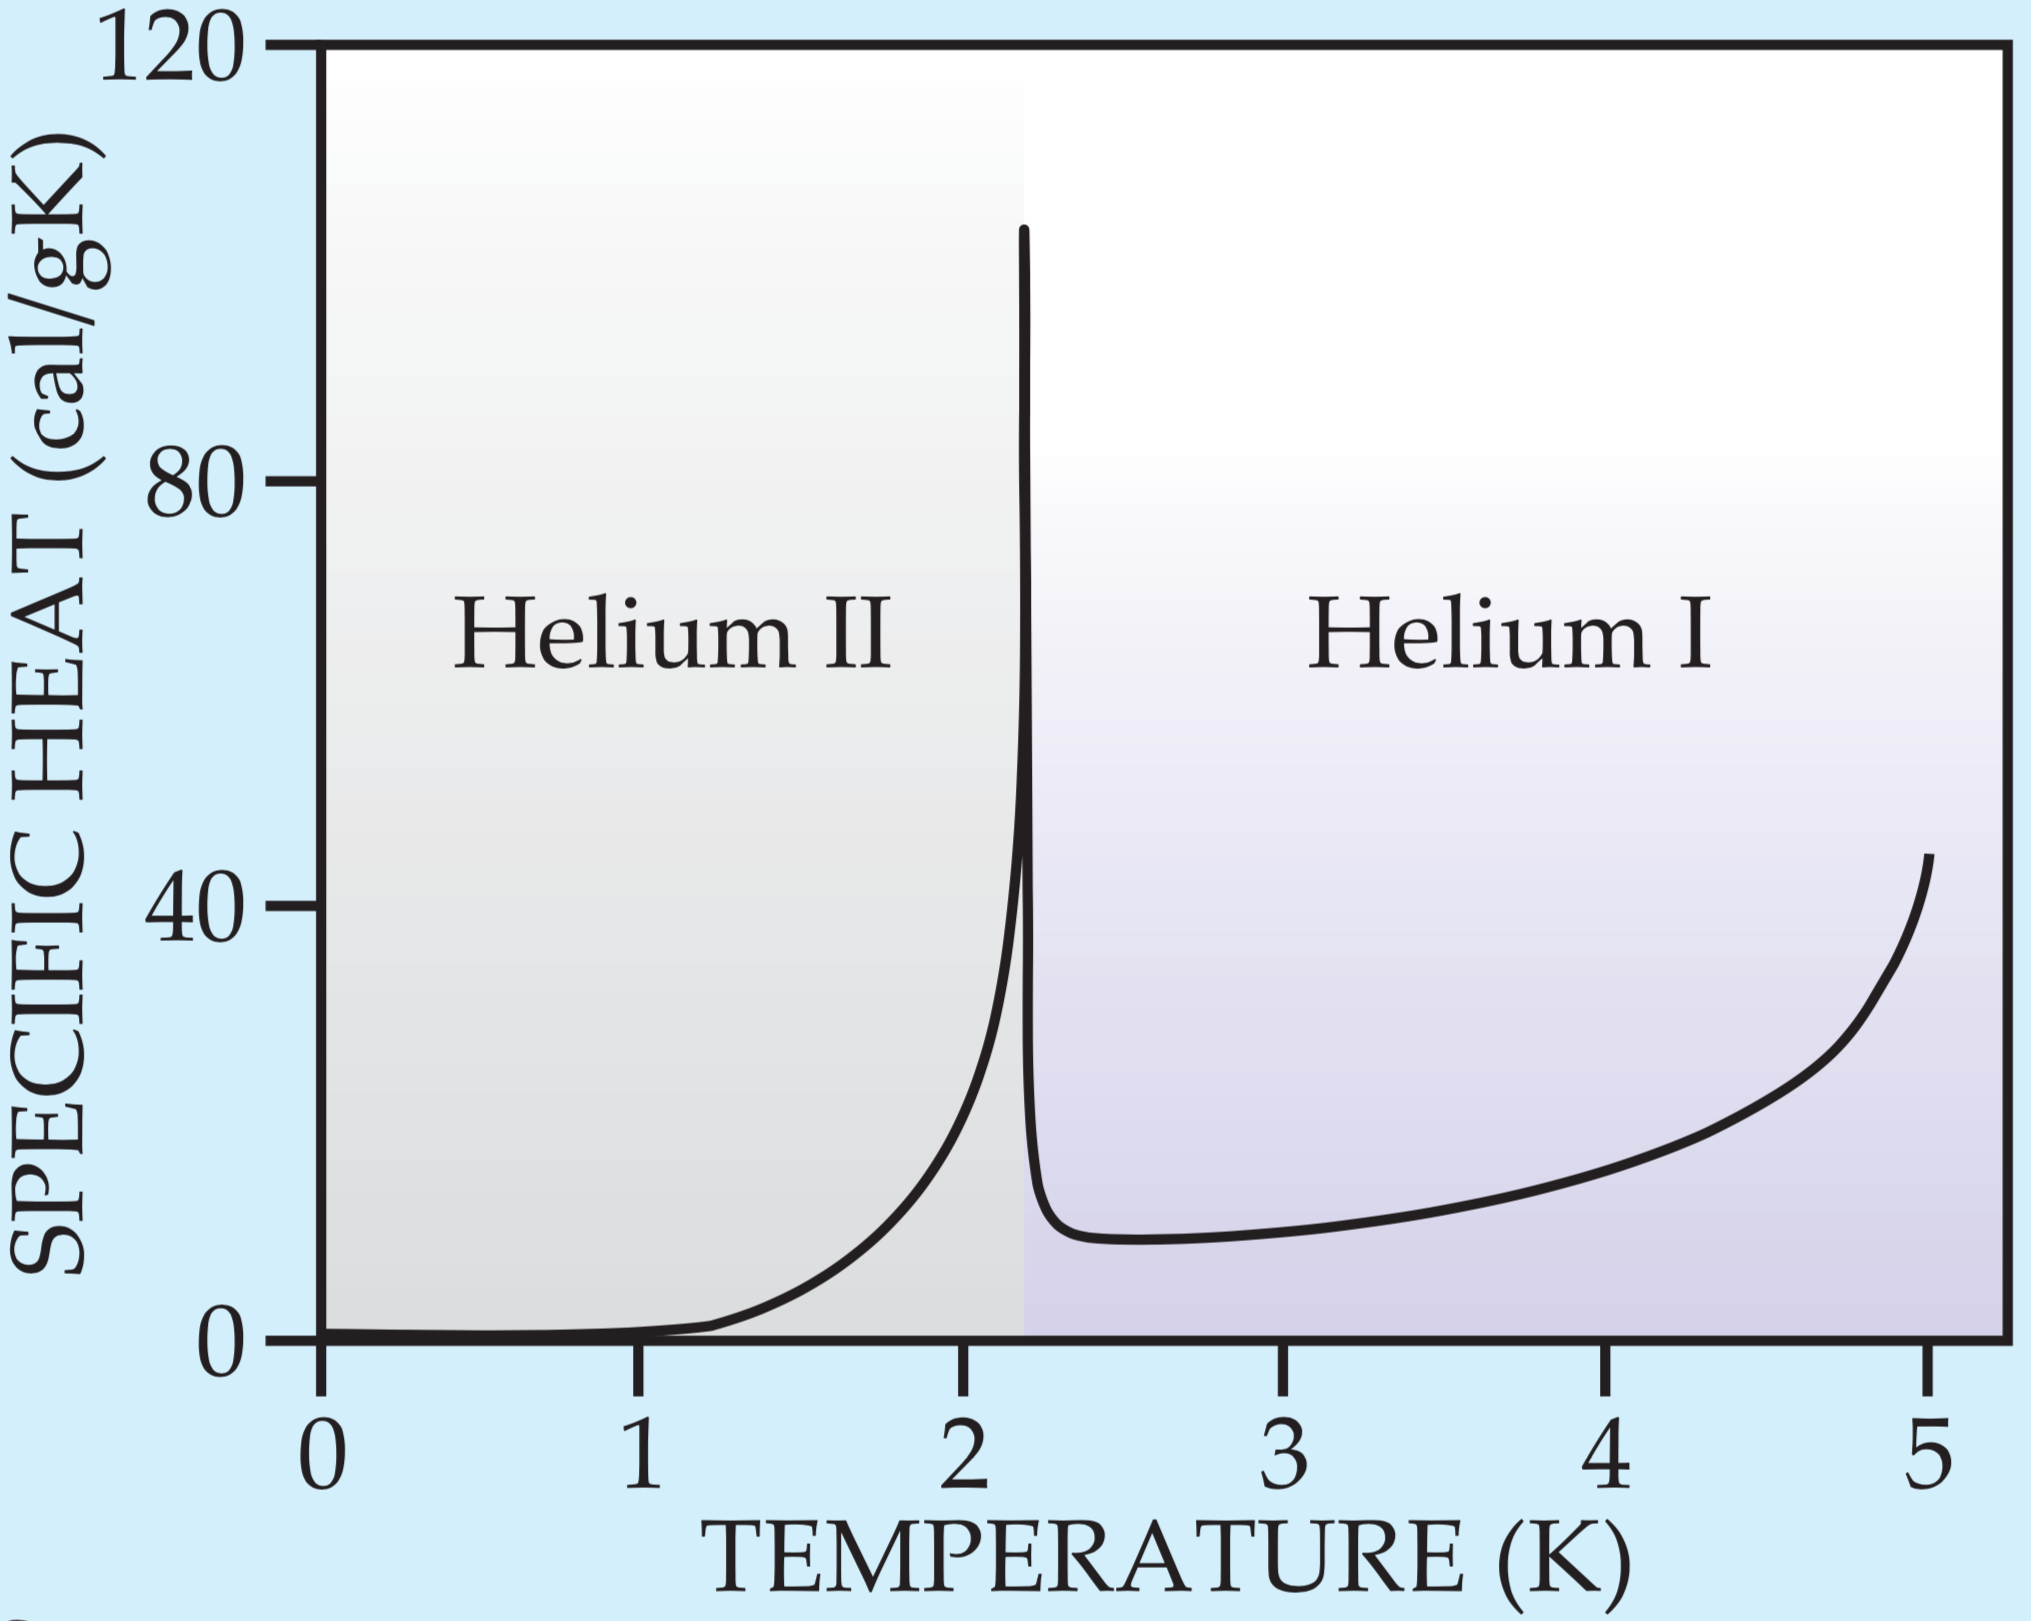
\includegraphics[width=0.75\textwidth]{specific-heat}
		\end{center}
		\caption{The specific heat of $^4$He as a function of the temperature. There is a clearly visible singularity around $2.2\unit{K}$ and the graph itself has the distinct $\lambda$-like shape that inspired\citep{Keesom1932} Willem and Anna Keesom to call the temperature at which the singularity occurs the ``$\lambda$-point''. (Illustration courtesy of R.J. Donnelly\citep{Donnelly2009})}
		\label{fig:specific-heat}
	\end{figure}	
	
	\section{A brief history of superfluidity}
		\lettrine[lines=3,findent=3pt,nindent=0pt]{H}{elium} was the last gas to be liquefied and was done so by Heike Kamerlingh Onnes in 1908\citep{Onnes1908,Onnes1909}. In 1932 John McLennan saw that liquid helium stopped boiling below $\approx\!2.2\unit{K}$\citep{McLennan1932} and later that year Willem Keesom and his daughter Anna observed, while measuring the temperature dependence of the specific heat, a singularity around the same temperature\citep{Keesom1932}. They called it the ``$\lambda$-temperature'',  $T_\lambda$, because of the shape of the temperature dependence of the specific heat resembling the Greek letter $\lambda$ (see Figure \ref{fig:specific-heat}). A few years later in 1935 Burton measured a sharp decrease in the viscosity of liquid helium below $T_\lambda$\citep{Burton1935}. Around the same time Fritz London was already thinking about macroscopic wave functions and why helium does not freeze at $T=0\unit{K}$ under atmospheric pressure\citep{London1935}. London and Simon concluded that it was caused by the zero point motion of the helium atoms and their associated kinetic energy that is comparable to their Van der Waals energy, effectively preventing liquid helium to solidify\citep{Simon1934,London1936}. The year after, in 1936, Willem and Anna Keesom measured an abnormally high heat conductance below $T_\lambda$\citep{Keesom1936}. This was confirmed roughly one year later by J.F. Allen \emph{et al.}\citep{Allen1937} and it was understood that the high thermal conductance was the reason for the helium to stop boiling whenever the temperature drops below $T_\lambda$. It was in 1937, when Kapitza tried to determine the viscosity of the laminar flow, that he measured a viscosity that was about $10^4$ times smaller than that of hydrogen gas\citep{Kapitza1938}. It was then that Kaptiza who, by analogy with superconductors, first coined the word ``superfluid''\citep{Kapitza1938} to describe the special state that helium enters below the $\lambda$-point where it can flow, seemingly without friction. Allen and Misener realised that superfluid helium is not just a liquid with a very low viscosity, but that its hydrodynamics was completely different from that of ordinary liquids\citep{Allen1938} and therefore required a completely new interpretation.\\
		
		The start of this new interpretation was made by London\citep{London1938} in 1938 when he made a connection between the behaviour of superfluid helium and that of an ideal ``Bose-Einstein'' (BE) gas. Both his calculated value for $T_c=3.09\unit{K}$ and the behaviour of the temperature dependence of the heat capacity for the ideal BE-gas were very similar to the measured ones for liquid helium below $T_\lambda$. He wrote to Nature that ``it was difficult not to imagine a connection with ``Bose-Einstein condensation'' (BEC). Tisza expanded upon London's ideas\citep{Tisza1938} and considered a Helium II system of total $N$ atoms to consist of two parts; a macroscopic ``condensed'' part $n_0$, the superfluid component, in the ground state, and the remaining part $n=N-n_0$, the normal component, where the helium atoms are distributed over the excited states. Assuming this was correct the fraction $n_0/N$ should decrease with increasing temperature according to the equation\\
		\begin{align}
			\frac{n_0}{N} = 1-\qty(\frac{T}{T_0})^s \quad \text{for} \quad T<T_0
		\end{align}
		where $s=3/2$ for an ideal gas and should be taken larger, e.g. $s=5$, for a real liquid with stronger interactions between the atoms.\\
		
		This was the birth of the ``two-fluid'' model. With this model he derived two hydrodynamic equations for liquid helium below $T_\lambda$ and discovered that within it, heat propagates in waves instead of diffusing through the medium, and calculated the velocity of these waves. He also explained why the viscosity is disappearing at low temperatures contrary to classical liquids where the viscosity increases\citep{Tisza1938-1,Tisza1938-2,Tisza1940-1,Tisza1940-2}. In 1941 Lev Landau reformulated Tisza's theory on a more rigorous footing\citep{Landau1941,Landau1949}. He assumed, contrary to Tisza, that the normal component of the liquid was made-up of collective excitations instead of excited single atoms. He postulated that the liquid could exhibit two states of motion which he called ``potential motion'' that is irrotational ($\curl{\vec{v}}=0$), and ``vortex motion'' that is rotational ($\curl{\vec{v}} \neq 0$). The corresponding energies of these two motions are discontinuously separated by an energy gap $\Delta$. In case of potential internal motion  the excitations are quanta of longitudinal (sound) waves, i.e., phonons. The excitations of the vortex-spectrum could be called ``rotons'' (see Figure \ref{fig:phonon-roton}).\\

		\begin{figure}[t]
			\begin{center}
				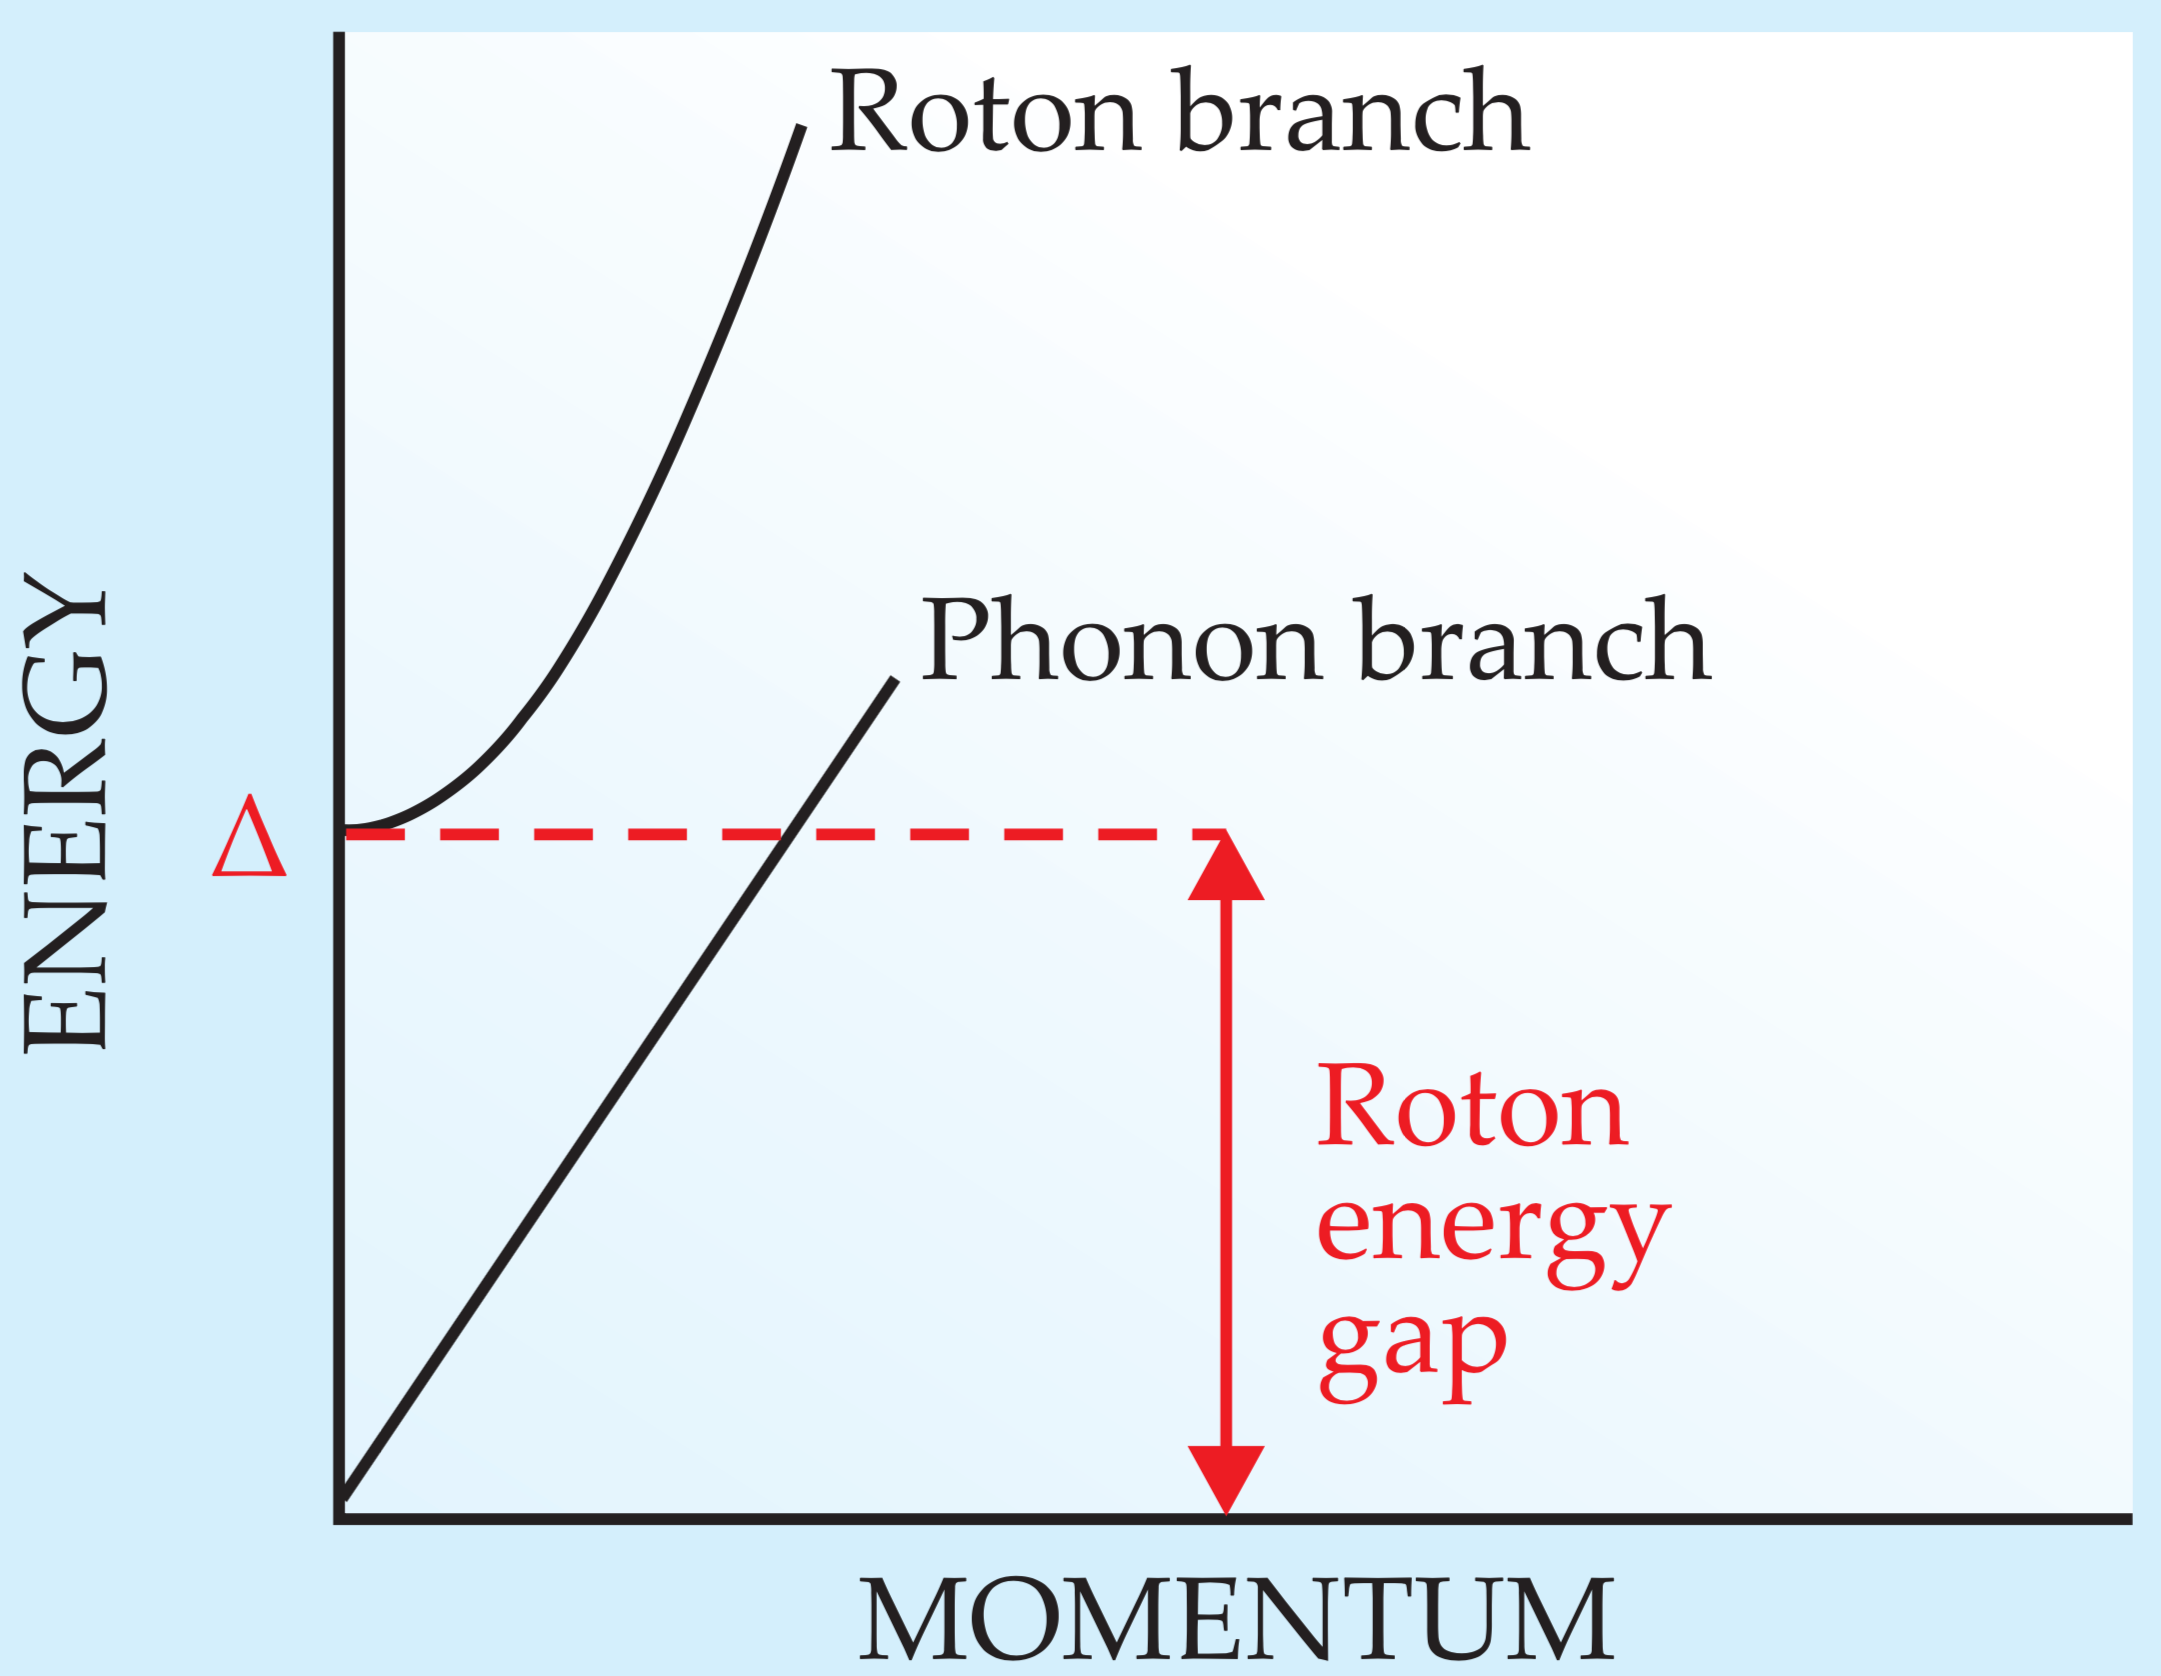
\includegraphics[width=0.495\textwidth]{phonon-roton-landau-first}
				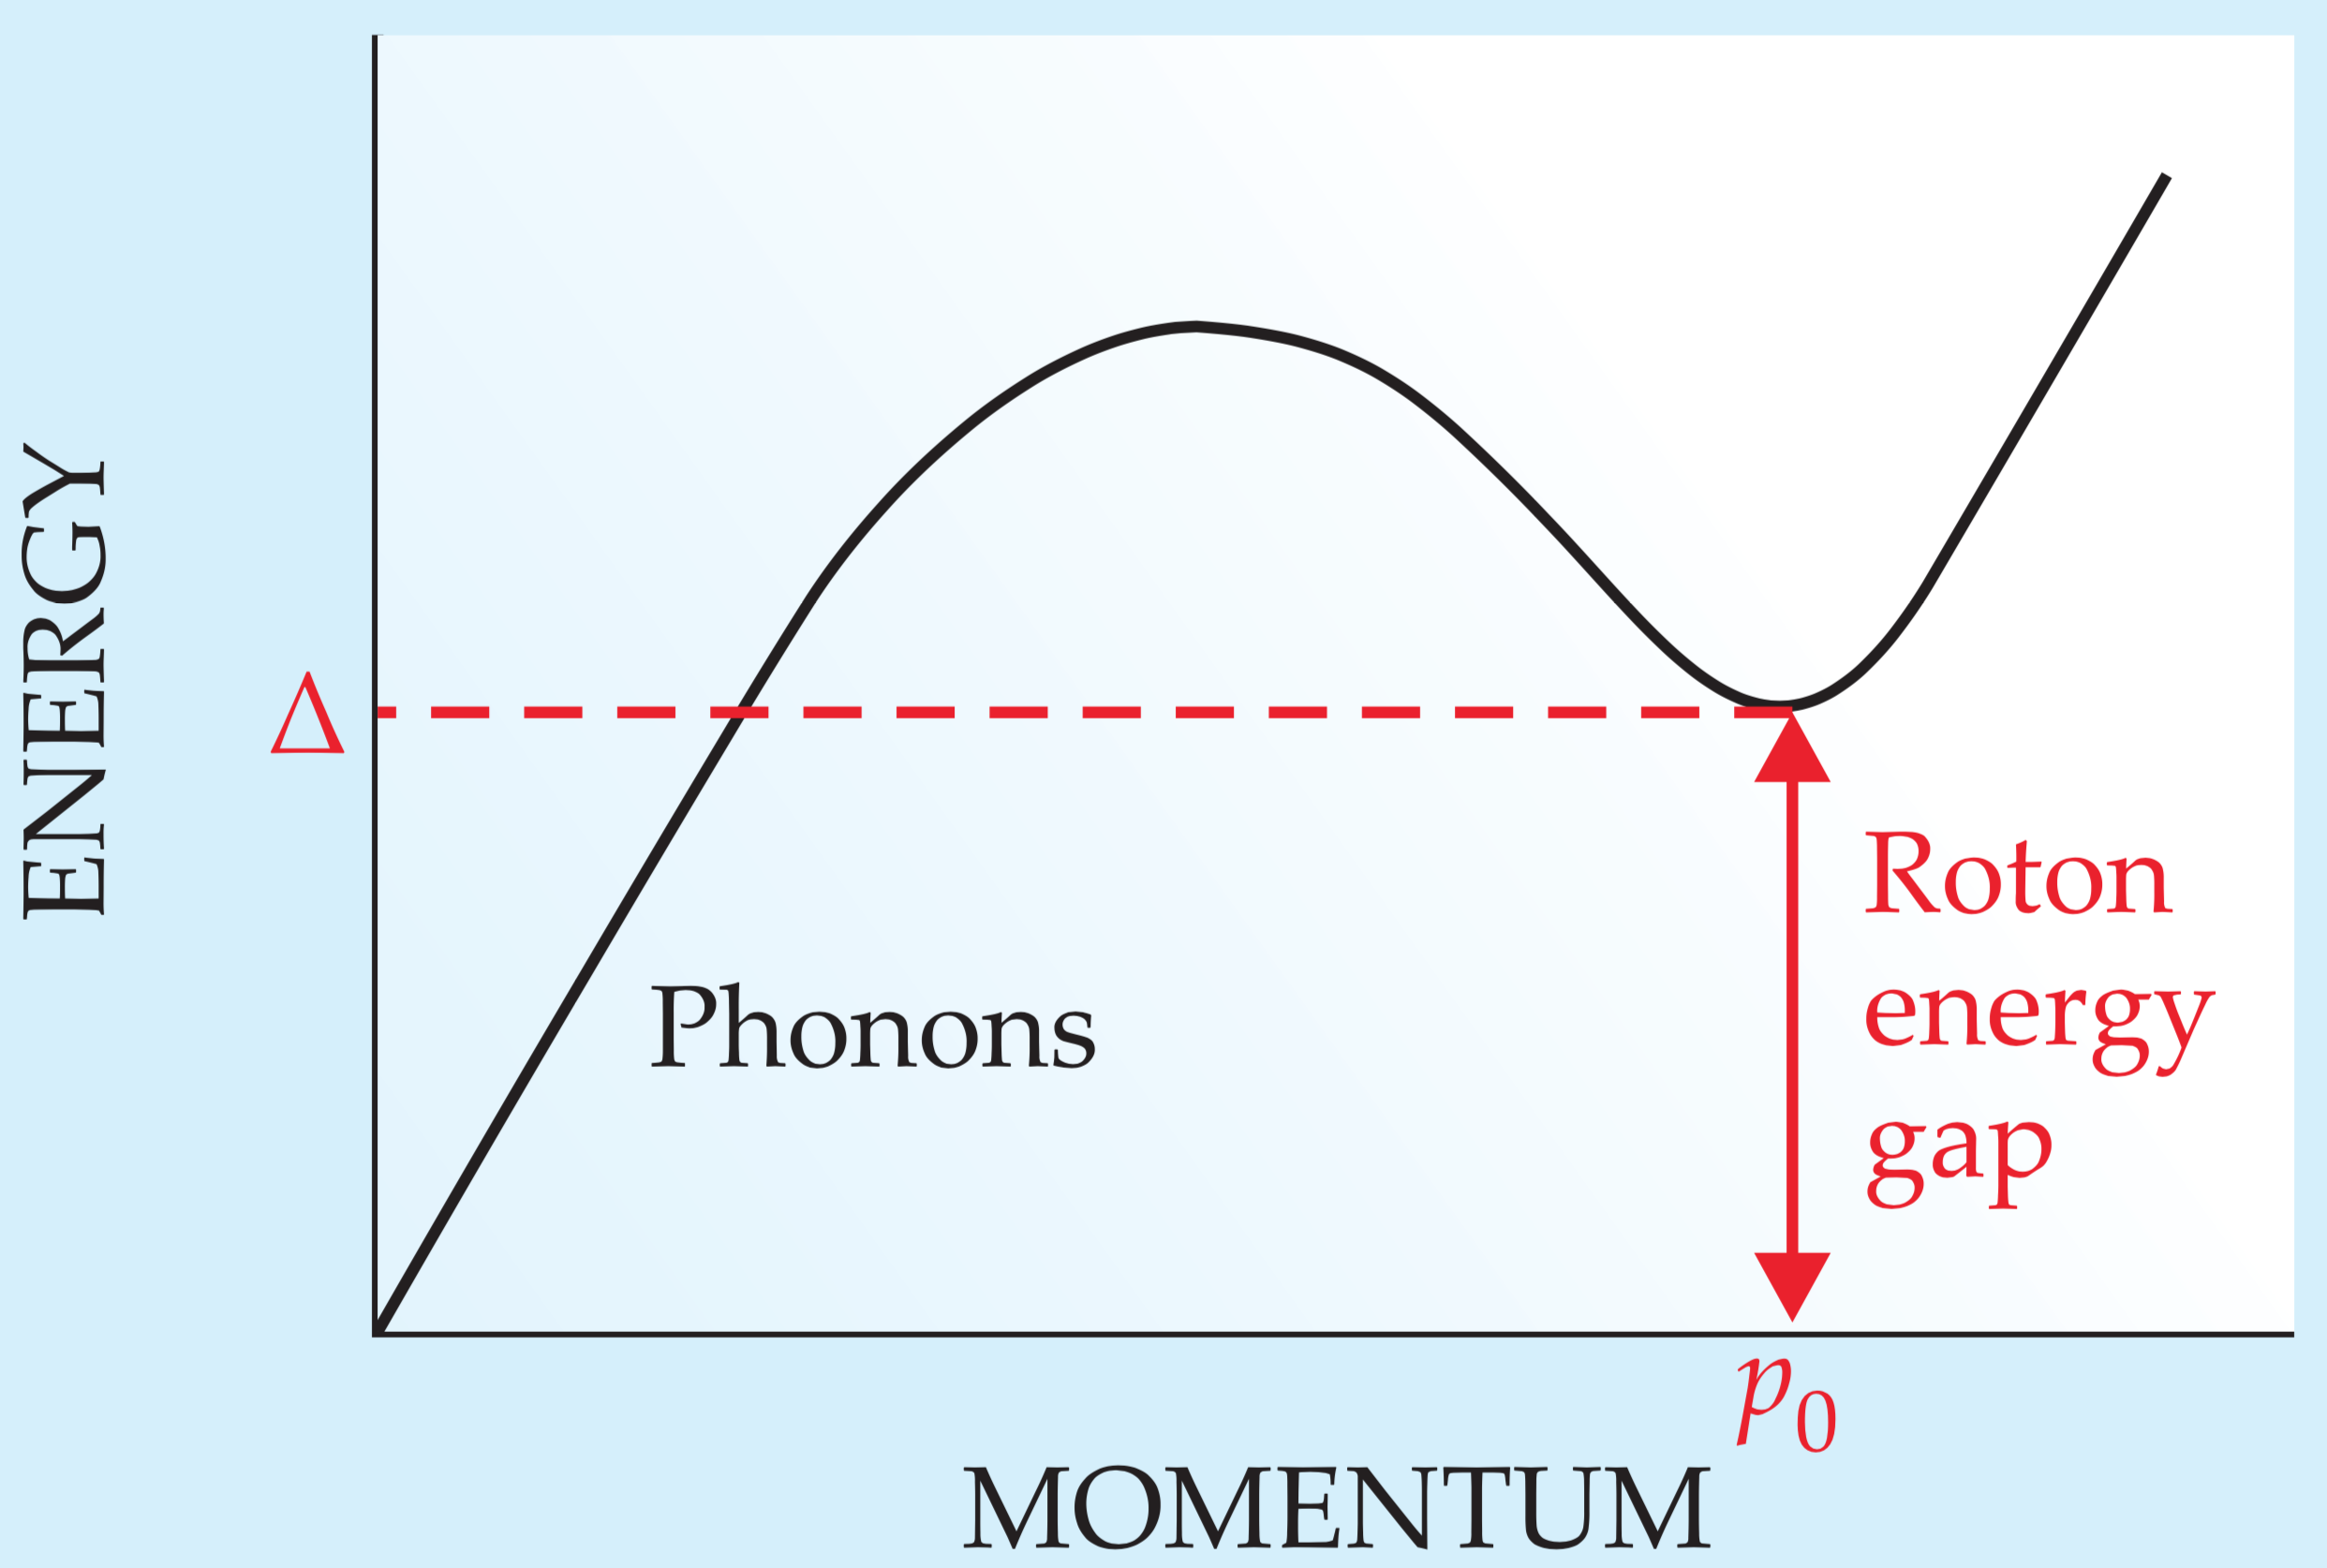
\includegraphics[width=0.495\textwidth]{phonon-roton-bogoliubov}
			\end{center}
			\caption{Left: Lev Landau's 1941 energy dispersion curve\citep{Landau1941} for the excitations in liquid helium below $T_\lambda$. It exhibits a phonon- and a roton branch. The slope of the linear phonon branch corresponds to the velocity of sound. Right: Lev Landau's 1947 modified dispersion curve. The roton-branch is no longer a separate excitation branch but rather an extension of the phonon-branch. (Illustration courtesy of R.J. Donnelly\citep{Donnelly2009})}
			\label{fig:phonon-roton}
		\end{figure}

		A theoretical demonstration, explicitly showing that phonons and rotons are collective excitations of the liquid, came in the form of a 1947 paper by Nikolay Bogolyubov\citep{Bogolyubov1947}. The intimate relationship between superfluidity and BEC was not universally accepted until 1995 when Cornell and Wienman in Colorado and Ketterle at MIT discovered BEC in rubidium quantum gases\citep{Cornell2002,Ketterle2002}.

	\section{Some key concepts}
		\lettrine[lines=3,findent=3pt,nindent=0pt]{I}{n} this section I will briefly introduce some key ideas that are used throughout the thesis and that are needed to fully appreciate the discussed material. Also references to more complete and more in-depth treatments will be provided for the interested reader.
		
		\subsection{Bose-Einstein condensation and long-range order}
			The essential concept of Bose-Einstein (BE) condensation is the fact that at low temperatures, multiple bosons, unlike fermions, will occupy the same quantum state. In theory there is no upper bound of how many bosons can occupy such a single state. It is then said that, with ever decreasing temperature, a macroscopic part of the total number of bosons will ``condense'' into the quantum state with the lowest energy.\\			
			
			Another important concept in BEC is the idea of long-range order. Let us start by introducing the one-body density matrix of a system of $N$ bosons in a pure state $\Psi_k(\vec{r}_1,\vec{r}_2,\ldots,\vec{r}_N)$
			\begin{align}
				n^{(1)}_k(\vec{r},\vec{r'}) \vcentcolon= N\int\!	\Psi_k^*(\vec{r},\vec{r}_2,\ldots,\vec{r}_N)\Psi_k(\vec{r'},\vec{r}_2,\ldots,\vec{r}_N)\diff{r}_2\diff{r}_3\ldots\diff{r}_N	\label{eq:def-obd-matrix}
			\end{align}
			where the integral is taken over the $N-1$ coordinates $\vec{r}_2,\vec{r}_3,\ldots,\vec{r}_N$. For a statistical mixture of quantum states one needs to take the weighted average over all the different $\Psi_k$-states. In thermodynamic equilibrium the states are Boltzmann weighted by their eigenvalues $\qty{E_k}$
			\begin{align}
				n^{(1)}(\vec{r},\vec{r'}) = \frac{1}{Q}\sum_k n^{(1)}_k(\vec{r},\vec{r'}) \unit{e}^{-E_k/k_BT}
			\end{align}
			where $Q$ is the partition function. For more general cases the one-body density matrix is defined
			\begin{align}
				n^{(1)}(\vec{r},\vec{r'}) \vcentcolon=\expval{\hat\Psi^\dagger(\vec{r})\hat\Psi(\vec{r'})}
			\end{align}
			where $\hat\Psi^\dagger(\vec{r})$/$\hat\Psi(\vec{r})$ are field-operators creating/annihilating a boson at $\vec{r}$ and the averaging $\expval{\cdots}$ is taken over all states in the mixture. Once it is accepted that a macroscopic part of the total number of bosons can occupy a single quantum state it can be demonstrated that, while considering a uniform isotropic sytem of $N$ bosons, the one-body density matrix (Eq. \ref{eq:def-obd-matrix}) tends to a constant value when the distance between $\vec{r}$ and $\vec{r}'$ goes to infinity. In the thermodynamic limit where $N,V\rightarrow\infty$ such that $n=N/V$ is kept fixed, the one-body density only depends on the modulus of the relative variable $\vec{s}:=\vec{r}-\vec{r}'$ so that we can write it as the Fourier transform of the momentum distribution as
			\begin{align}
				n^{(1)}(s) = \frac{1}{V}\int \! n^{(1)}\qty(\vec{p})\exp(i\vec{p}\cdot\vec{s}/\hbar)\,\mathrm{d}\vec{p} \label{eq:one-body-den-mom}
			\end{align}
			For a BEC system, the momentum distribution at small momenta is not smooth but has a sharp peak around $p=0$ for the bosons that are in the ground state, while the remaining bosons are smoothly distributed over the excited states.
			\begin{align}
				n(\vec{p})=N_0\delta(\vec{p})+\tilde{n}(\vec{p})
			\end{align}
			where $\tilde{n}$ is a smoothly varying function of $\vec{p}$. When this expression is plugged into Eq. (\ref{eq:one-body-den-mom}) and taking the limit where $s$ goes to infinity
			\begin{align}
				\lim_{s\rightarrow\infty}n^{(1)}(s)=\frac{N_0}{V},
			\end{align}
			where $N_0/V \vcentcolon= n_0\leq 1$ is called the condensate fraction. It is called long-range order since it involves the off-diagonal elements of the one-body density matrix; the elements that are usually associated with the coherences.\\
			
			A set of eigenvalues \{$n_i$\} of the one-body density matrix can be defined through the following eigenvalue equation
			\begin{align}
				\int \! n^{(1)}(\vec{r},\vec{r'})\varphi_i(\vec{r'}) \,\mathrm{d}\vec{r'} = n_i\varphi_i(\vec{r})
			\end{align}
			and its solutions \{$\varphi_i$\} form a natural orthonormal basis set of single boson wave functions $\int\!\varphi_i^*\varphi_j\,\mathrm{d}\vec{r}=\delta_{ij}$, with normalisation condition $\sum_i n_i=N$. This permits writing the on-body density matrix in a useful diagonalised form and recalling that BEC occurs when a single particle state $\varphi_i$ is occupied in a macroscopic way, say when $n_{i=0}=N_0$, a number of order $N$, we separate the condensate part from the rest
			\begin{align}
				n^{(1)}(\vec{r},\vec{r'}) = N_0\varphi_0^*(\vec{r})\varphi_0(\vec{r'})+\sum_{i\neq0}n_i\varphi_i^*(\vec{r})\varphi_i(\vec{r'}) \label{eq:obdm-diag}
			\end{align}

		\subsection{Bogolyubov's approximation and the order parameter}\label{sec:bogol-order}
			It is customary, given the importance of the condensate fraction $N_0$ in a BEC, to write the field operator of a $N$-body boson system as the sum of the condensate part and the rest, just as the one-body density matrix
			\begin{align}
				\hat{\Psi}(\vec{r})=\varphi_0(\vec{r})\hat{a}_0 + \sum_{i\neq 0} \varphi_i(\vec{r})\hat{a}_i \label{eq:field-operator}
			\end{align}
			where the $\hat{a}_i$ and $\hat{a}_i^\dagger$ are annihilation and creation operator of a particle in state $\varphi_i$ and obey the usual bosonic commutation relations
			\begin{align}
				\commutator{\hat{a}_i}{\hat{a}_j^\dagger}=\delta_{ij},\quad 	\commutator{\hat{a}_i}{\hat{a}_j}=0=\commutator{\hat{a}_i^\dagger}{\hat{a}_j^\dagger}
			\end{align}
			Using Eq. (\ref{eq:field-operator}) in Eq. (\ref{eq:def-obd-matrix}) and comparing it to Eq. (\ref{eq:obdm-diag}) one finds the expectation value of $\expectationvalue{\hat{a}_j^\dagger\,\hat{a}_i}=\delta_{ij}n_i$. Now, the Bogolyubov approximation essentially replaces the operators $\hat{a}_0$ and $\hat{a}_0^\dagger$ with the $c$-number\footnote{The term $c$-number is old nomenclature for a classical number, which can be real or complex, to distinguish them from quantum numbers, or $q$-numbers, that are represented by operators.} $\sqrt{N_0}$. This is equivalent to ignoring the non-commutative nature of the operators due to the macroscopic occupation of the state $\varphi_0$, when $N_0=\expectationvalue{\hat{a}_0^\dagger\,\hat{a}_0}\gg 1$. We then rewrite the field operator as the sum of a classical field for the condensed component and quantum field for the non-condensed component
			\begin{align}
				\hat{\Psi}(\vec{r})=\Psi_0(\vec{r})+\delta\hat{\Psi}(\vec{r}),\label{eq:order-param-real}
			\end{align}
			where $\delta\hat{\Psi}(\vec{r})=\sum_{i\neq 0}\varphi_i(\vec{r})\hat{a}_i$ and $\Psi_0(\vec{r})=\sqrt{N_0}\varphi_0(\vec{r})$. At $T=0$ the whole system is condensed and one can ignore $\delta\hat{\Psi}$ altogether; the field operator becomes a normal function of space $\Psi_0$.\\
			
			The classical field $\Psi_0$ is called the \emph{effective}- or \emph{macroscopic} wave function of the condensate and it behaves like an order parameter in the sense that it varies continuously between a maximum value $\sqrt{N}$, that is proportional to the total number particles in the system, at $T=0$, and vanishes at the superfluid-normal fluid phase transition temperature $T_\lambda$. It is a complex quantity characterised by a real-valued modulus and phase $S$:
			\begin{align}
				\Psi_0(\vec{r}) = \absolutevalue{\sqrt{N_0}\varphi_0(\vec{r)}}\,\mathrm{e}^{iS(\vec{r})}\label{eq:order-param-complex}
			\end{align}
			The modulus determines the number-density of the condensate, while the phase $S$ plays an important role in the coherence and properties of the superfluid. As we will see in Section \ref{sec:rot-vort}, $S$ plays the role of a velocity potential.\\
			
			Using an order parameter as defined here is equivalent to using the many-body wave function
			\begin{align}
				\Phi(\vec{r}_1,\vec{r}_2,\ldots\vec{r}_N)=\prod_{i=1}^{N}\varphi_0(\vec{r}_i),
			\end{align}
			with a density operator $\hat{\rho}(\vec{r}) \vcentcolon= \sum_{i=1}^{N}\delta(\vec{r}-\vec{r}_i)$ (see Section \ref{sec:dft-method}). One way to see why this wave function plays the role of an order parameter is to look at its time dependence. For normal wave functions the time dependence is determined by the eigenvalues $E_i$ of the Hamiltonian of the system
			\begin{align}
				\Psi(\vec{r},t)=\psi(\vec{r})\,\mathrm{e}^{-iE_it/\hbar}
			\end{align}
			But in this case, the time dependence is determined by the chemical potential $\mu=E(N)-E(N-1)\approx \partial E/\partial N$
			\begin{align}
				\Psi_0(\vec{r},t)=\Psi_0(\vec{r})\,\mathrm{e}^{-i\mu t/\hbar} \label{eq:td-order-param}
			\end{align}
			Another aspect of $\Psi_0$ being an order parameter and not a true many-body wave function is that two solutions $\Psi_a$ and $\Psi_b$ of the non-linear droplet Hamiltonian corresponding to two different values of the chemical potential $\mu_a$ and $\mu_b$ are not necessarily orthogonal, i.e. $0 \leq N^{-1}\int\!\Psi_a^*\Psi_b\unit{d}\vec{r} < 1$. However, in dilute gases it is possible to construct a many-body wave function from the order parameter that regains its orthonormality in the thermodynamic limit
			\begin{align}
				\Phi_0(\vec{r}_1,\vec{r}_2,\ldots,\vec{r}_N) = \qty(\frac{1}{\sqrt{N}}\Psi_0(\vec{r}_1))\qty(\frac{1}{\sqrt{N}}\Psi_0(\vec{r}_2))\cdots\qty(\frac{1}{\sqrt{N}}\Psi_0(\vec{r}_N))
			\end{align}
			
		\subsection{Landau's criterion for superfluidity}
			\begin{figure}[t]
				\begin{center}
					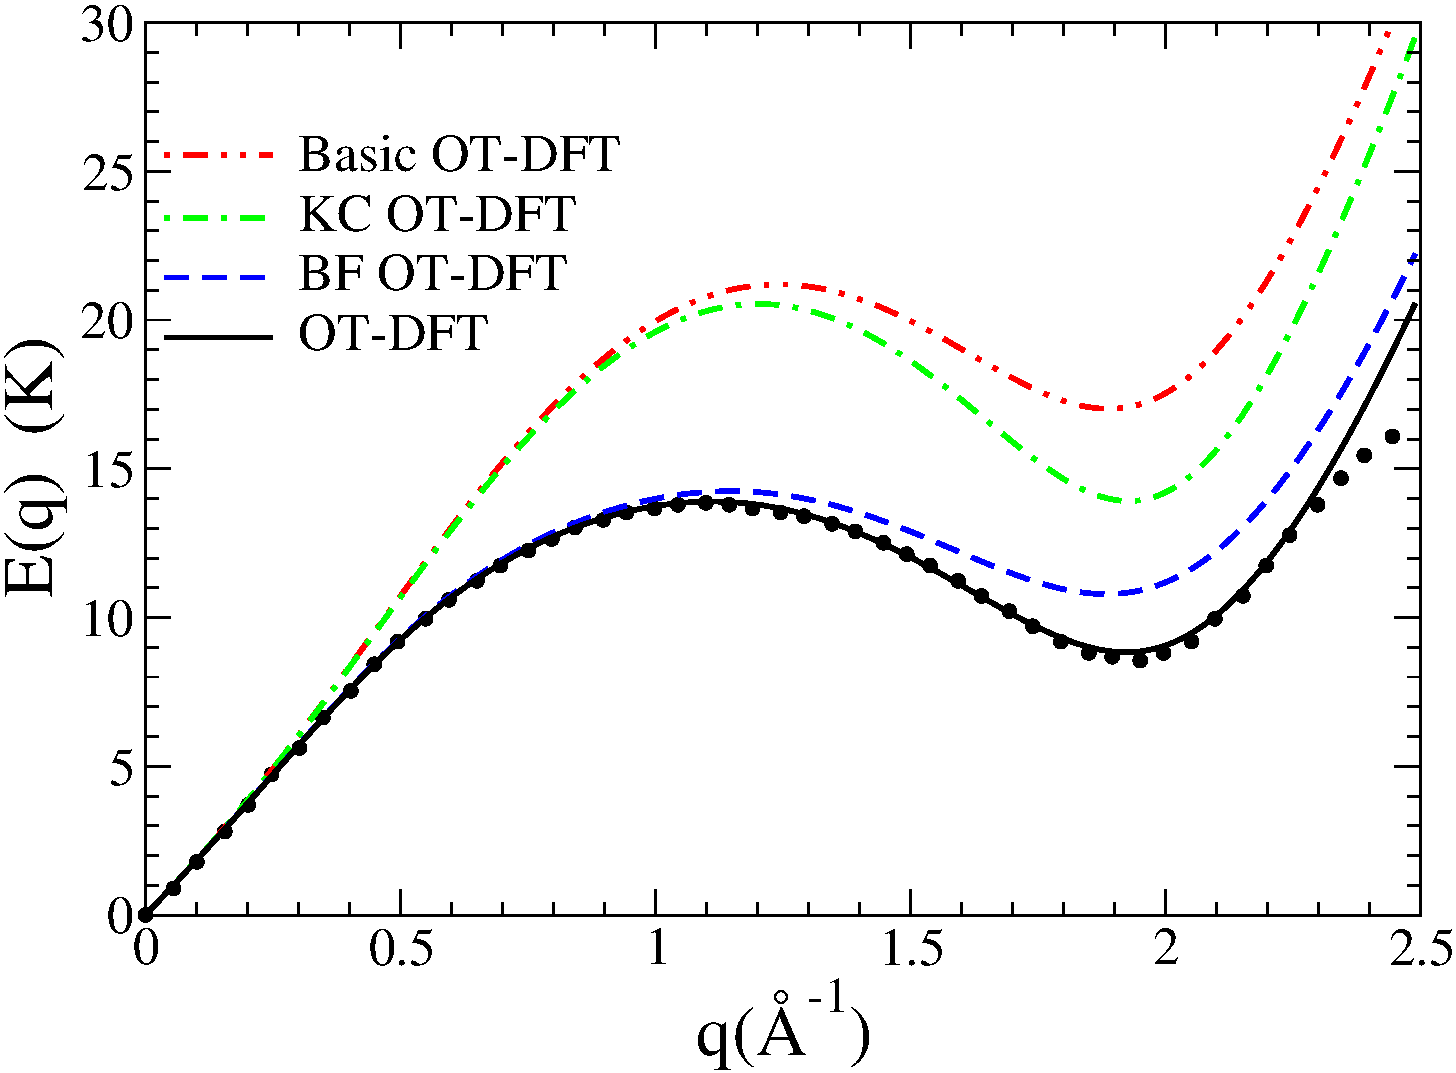
\includegraphics[width=0.9\textwidth]{dispersion-relation}
					\caption{Dispersion relation for elementary excitations in liquid $^4$He calculated as in  \cite{Mat10a}. `Basic' indicates the OT-DFT without the non-local kinetic energy correlation (KC) nor the back-flow (BF) terms; KC OT-DFT adds  to the basic OT-DFT the KC term; BF OT-DFT adds to the basic OT-DFT the BF term. The dots are the experimental data from \cite{Don81}. The Landau velocity $v_L = E(q)/(\hbar\,q)|_{min}$ obtained for each functional is  60.3 m/s (OT-DFT); 75.1 m/s (BF OT-DFT); 94.4 m/s (KC OT-DFT); 118 m/s (basic OT-DFT); and 57.5 (experiment).}
					\label{fig:dispersion-relation}
				\end{center}
			\end{figure}
		
			For a gas or liquid to be able to become superfluid Landau postulated that the energy dispersion relation needs to fulfil certain requirements. Specifically for a fluid to flow  without dissipation, i.e. a super-flow, the velocity field needs to fulfil the following inequality:
			\begin{align}
				v<v_c = \min_{\vec{p}}\frac{\epsilon(\vec{p})}{p}
			\end{align}
			
			For an ideal Bose gas $\epsilon(\vec{p})= \frac{p^2}{2m}$. In this case 
			\begin{align}
				v_c &= \min_{\vec{p}}\frac{\epsilon(\vec{p})}{p} \\
					&= \min_{\vec{p}}\frac{p}{2m} \\
					&= 0
			\end{align}
			Apparently ideal Bose-gases cannot become superfluid.\\
			
			But if we allow for some weak interactions between the bosons the energy dispersion relation is given by
			\begin{align}
				\epsilon(\vec{p})=\sqrt{\frac{gn}{m}p^2+\qty(\frac{p^2}{2m})^2},
			\end{align}
			Bogolyubov's dispersion law for elementary excitations (1947). And thus
			\begin{align}
				v_c &=\min_{\vec{p}}\sqrt{\frac{gn}{m}+\frac{p^2}{4m^2}} \\
					&= \sqrt{\frac{gn}{m}} \\
					&= c,
			\end{align}
			the speed of sound. Here $g=\frac{4\pi\hbar^2a}{m}$, and $a$ the $s$-wave scattering length. The weakly interacting Bose gases can become superfluid.\\			

			Liquid helium below the $\lambda$-point has a similar energy dispersion relation (see Figure \ref{fig:dispersion-relation}) hence reinforcing the notion that superfluidity and Bose--Einstein condensation are two intimately related concepts. The experimental value of the speed of sound is $\sim\!57.5\unit{m/s}$.
			
		\subsection{Rotation and vorticity in superfluids}\label{sec:rot-vort}
			\begin{figure}[t]
				\begin{center}
					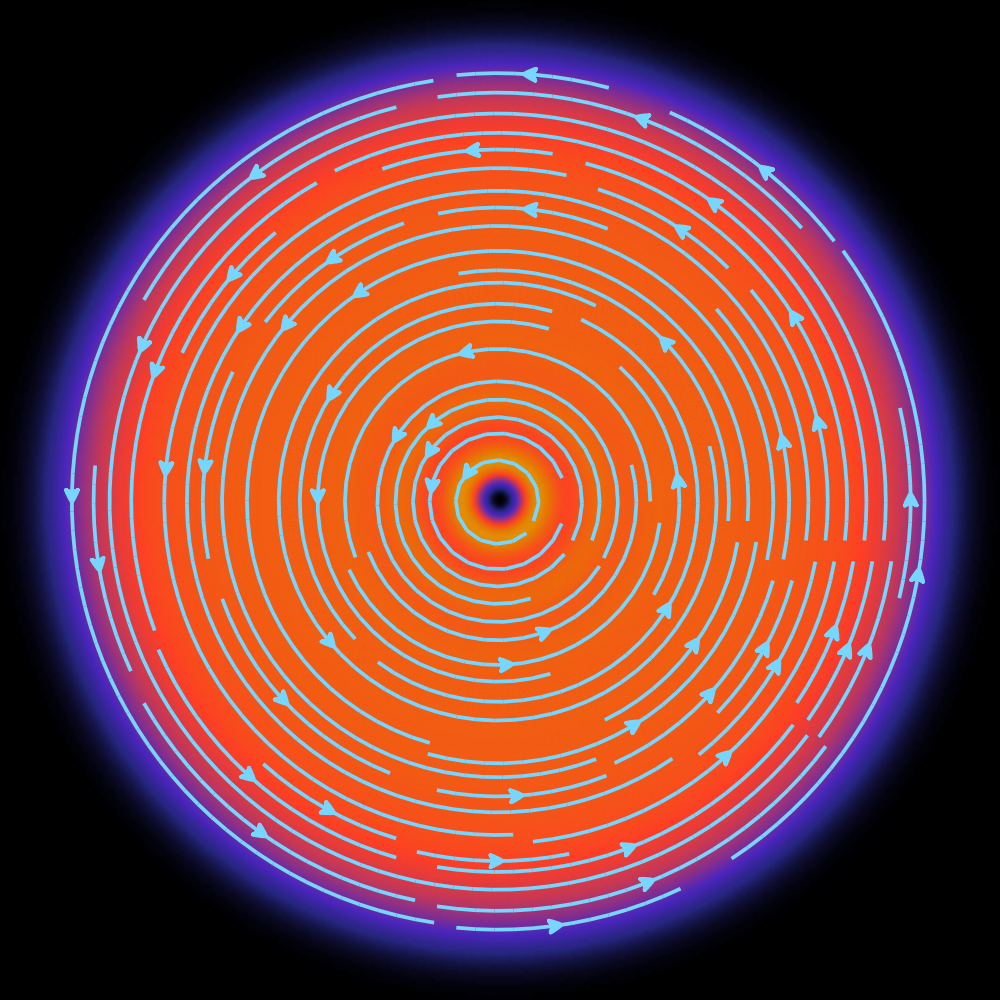
\includegraphics[width=0.5\textwidth]{vortex-xy}
					\caption{Cross section of a $^4$He droplet through a symmetry plane. The droplet is made of 1000 atoms. Superimposed in cyan are the streamlines of the velocity field $\vec{v}_s$ for $s=1$. They are concentric circles, centred around the vortex core along the $z$-axis. The colour scale encodes for the density $\rho(r)$. The radius of the droplet is about 22\,\AA.}
					\label{fig:vortex-xy}
				\end{center}
			\end{figure}
		
			Starting from time-dependent Euler-Lagrange (EL) equation (Eq. \ref{eq:td-el-equation}, see Chapter \ref{sec:dft-method}) for the time-evolution of the order parameter $\Psi$ (Eq. \ref{eq:order-param-complex}, dropping the ground-state subscript and allowing $\varphi$ and $S$ to vary in time)
			\begin{align}
				i\hbar\frac{\partial}{\partial t} \Psi({\mathbf r},t) = \left[-\frac{\hbar^2}{2m}\laplacian + \frac{\delta{\cal E}_{c}}{\delta\rho}\right]\Psi(\textbf{r},t)
			\end{align}
			one left-multiplies it with the complex conjugate of the order parameter $\Psi^*$ and then subtract the complex conjugate of the whole expression on both sides. After some algebra and defining $\rho(\vec{r},t)\vcentcolon=N\abs{\varphi(\vec{r},t)}^2$, one arrives at the continuity equation
			\begin{align}
				\frac{\partial\rho}{\partial t} + \div{\vec{j}}=0, \label{eq:continuity-eq}
			\end{align}
			with
			\begin{align}
				\vec{j}(\vec{r},t) \vcentcolon=& -\frac{i\hbar}{2m}\qty\big[\Psi^*(\vec{r},t)\grad{\Psi}(\vec{r},t) - \Psi(\vec{r},t)\grad{\Psi^*}(\vec{r},t)] \\
					=&\,\rho(\vec{r},t)\frac{\hbar}{m}\grad{S(\vec{r},t)}
			\end{align}
			From Eq. (\ref{eq:continuity-eq}) it follows that the atomic number density is a conserved quantity.\\
			
			We can identify the collective velocity $\vec{v}_s$ of the superfluid through the relation
			\begin{align}
				\vec{v}_s(\vec{r},t) = \vec{j}/\rho=\frac{\hbar}{m}\grad{S(\vec{r},t)} \label{eq:velocity-field}
			\end{align}
			and we see that the rotation of the velocity field of the superfluid $\curl{\vec{v}_s}=0$, i.e. the fluid is said to be \emph{irrotational}; a typical property of superfluids. Conversely, taking the curl $\curl{\vec{j}}=\frac{\hbar}{m}\grad{\rho}\times\grad{S}$ we see that this is merely a restatement of the fact that one needs a gas or liquid with a non-uniform density and a non-zero phase for it to be able to support vortices.\\
			
			Let us consider the illustrative example of a line vortex through the origin along the $z$-axis. As will be demonstrated in Section \ref{sec:vortical-states}, this is a stationary state of the droplet Hamiltonian and therefore its time dependence is just a multiplicative factor. In cylindrical coordinates $(r,\varphi,z)$ such a vortex solution has the form
			\begin{align}
				\Psi_s(\vec{r}) = \sqrt{\rho(r)}\unit{e}^{is\varphi}, \label{eq:line-vortex}
			\end{align}
			with $s$ an integer. This is an eigenfunction of the angular momentum operator $\hat{L}_z$ with eigenvalue
			\begin{align}
				\hat{L}_z \Psi_s(\vec{r}) &= \frac{\hbar}{i}\frac{\partial}{\partial\varphi}\Psi_s(\vec{r}) = \hbar s\Psi_s(\vec{r})
			\end{align}
			and with expectation value
			\begin{align}
				\expval{\hat{L}_z} &= \expval{\hat{L}_z}{\Psi_s} \\
					&= \hbar s \braket{\sqrt{N_0}\varphi_0} \\
					&= N_0\hbar s
			\end{align}
			The angular momentum is quantised and proportional to the number of bosons in the BEC fraction/superfluid. We can calculate the velocity field
			\begin{align}
				\vec{v}_s = \frac{\hbar}{m}\grad{S} = \frac{\hbar}{m}\frac{s}{r}\,\vu*{\varphi}
			\end{align}
			The streamlines of $\vec{v}_s$ are concentric circles, centred around the z-axis, lying in the $xy$-plane (see Figure \ref{fig:vortex-xy}). Contrary to rigid rotation fields which increase proportional to the distance from the $z$-axis $r$, the superfluid rotation field decreases proportional to distance from the $z$-axis $1/r$ and is singular in the origin. Calculating the circulation of the velocity field $\vec{v}_s$ along a closed contour including the $z$-axis gives
			\begin{align}
				\oint_{\partial\Sigma}\!\vec{v}_s\cdot\unit{d}\vec{l} &=
				\int_{0}^{2\pi}\!\frac{\hbar}{m}\frac{s}{r}\,\vu*{\varphi}\cdot r\unit{d}\varphi\,\vu*{\varphi} \\
					&= 2\pi s\frac{\hbar}{m}
			\end{align}
			There are two things to note here. Firstly, the circulation around a closed loop that encompasses the $z$-axis is quantised in units of $\hbar/m$ for $s\in\mathbb{N}_{>0}$. Secondly, the value of the circulation of the velocity field does not depend on the chosen contour as long as it includes the location of the vortex. This means that all the vorticity is contained at the location where the velocity field is singular (the ``core'' of the vortex), at $r=0$ along the $z$-axis.\\
			
			Because of the pole in the velocity field, Stokes theorem will lead to the following contradiction
			\begin{align}
				2\pi s\frac{\hbar}{m}=\oint_{\partial\Sigma}\!\!\!\vec{v}_s\cdot\unit{d}\vec{l} = \iint_{\Sigma}\!\curl{\vec{v}_s}\cdot\unit{d}\vec{\Sigma} = 0
			\end{align}
			and can therefore not be applied. To emphasise that all the vorticity is concentrated around the vortex core one can write formally
			\begin{align}
				\curl{\vec{v}_s} = 2\pi s\frac{\hbar}{m}\delta^{(2)}(\vec{r}_\perp)\,\vu{z},
			\end{align}
			where $\delta^{(2)}$ is 2-dimensional Dirac-delta function and $\vec{r}_\perp$ a vector in a plane perpendicular to the vortex line.\\

	\section{Helium droplets}
		\lettrine[lines=3,findent=3pt,nindent=0pt]{U}{ntil} the 1980, most experimental and theoretical work was done on bulk systems, i.e. systems of the order of $N_A$ number of atoms. It was only in the last couple of decades that advancements in technology enabled experimentalists to create nanoscale sized superfluid helium droplets. From the early 1990's onwards, superfluid helium nano-droplets became an active field of study, both experimentally and theoretically. 
		
		\paragraph{Finite size effects} Helium nanodroplets are considered ideal model systems to explore quantum hydrodynamics in self-contained, isolated superfluids. The main focus has been on the evolution of their properties with the number of atoms in the cluster, until the condensed matter limit is reached. Helium clusters are especially interesting in that quantum effects play a key role in determining their properties. In particular, given that a helium cluster is an ensemble of bosons at about 0.4 K [1, 2], manifestations of collective behaviour (such as superfluidity) are expected. On the other hand, it is not yet clear how the finite size of a cluster affects this non-classical (or degenerate) collective behaviour.

		\paragraph{Non-classical ideas} to explain, for example the capture of Cs atoms by large helium clusters, were introduced as early as 1986 [3], while recently, Toennies et al. [4] have measured the electronic spectrum of glyoxal molecules embedded in He clusters and found it consistent with a theoretical simulation computed using the phonon dispersion curve of superfluid bulk He II. The authors themselves, however, point out that at the average cluster size of 5500 He atoms reported in [4], the phonon dispersion curve is well in the bulk limit (see also [5, 6]); it is therefore not surprising that they find results consistent with the bulk case, especially for a molecule readily solvated inside the cluster, for which surface effects play a minor role. Therefore the influence on superfluidity of the He clusters size has not been detected so far.
		
		\paragraph{Properties of He droplets are difficult to determine} The helium-helium interaction is already weak in bulk liquid helium and in finite self-bound systems such as droplets it is even weaker, e.g. the binding energy per atom is $<\!7.17\unit{K}$. Because of this helium droplets cool down very rapidly due to fast evaporation and therefore reaching their limiting temperature of about $0.38\unit{K}$ in microseconds. Pure helium droplets are neutral systems and their properties like their size, binding energy and excitation spectra, are not easy to determine experimentally and are usually obtained by indirect methods. This didn't stop the theoreticians describe doped $^4$He$_N$ droplets using a wide variety of approaches depending on the size and character of the droplets ranging from Quantum Monte Carlo, Hypernetted-Chain/Euler-Lagrange, Variational Monte Carlo and many others.\\
	
		\paragraph{He droplets will pickup any dopant} A key property of helium droplets, in contrast to bulk helium, is their ability to pickup any kind of dopants with which they collide. Depending on the strength of the dopant-$^4$He interaction and the surface tension of the droplet, a dimensionless parameter $\lambda$ can be defined\citep{Anc95} with a critical value $\lambda_0\sim1.9$. Below $\lambda_0$ impurities are bound to the surface of the droplet (e.g. the alkalies), and above get solvated into the droplet's interior. They can therefore be doped with almost any kind of atomic- or molecular species where they can form new complexes.\\
		
		This enables a broad spectrum of possible experimental study. Due to the fact that helium droplet are ultra cold superfluid liquids, and therefore provide high mobility of any picked-up dopants, one can do high resolution spectroscopy studies. Having a fine control over the number of picked-up dopants[29] one can use droplets as a matrix for creating self-organising structures of polar molecules, or very cold metal clusters and study their Coulomb explosion.\\
		
		From the perspective of the droplet it's possible to use the dopants as gentle probes to determine the superfluid properties of helium droplets that would be inaccessible with other methods. For two examples of this see [37-39], where a dopant is used to probe the superfluid character of small $^4$He droplets and [16,17] to see their limiting temperatures.
		
		\begin{figure}[t]
			\begin{center}
				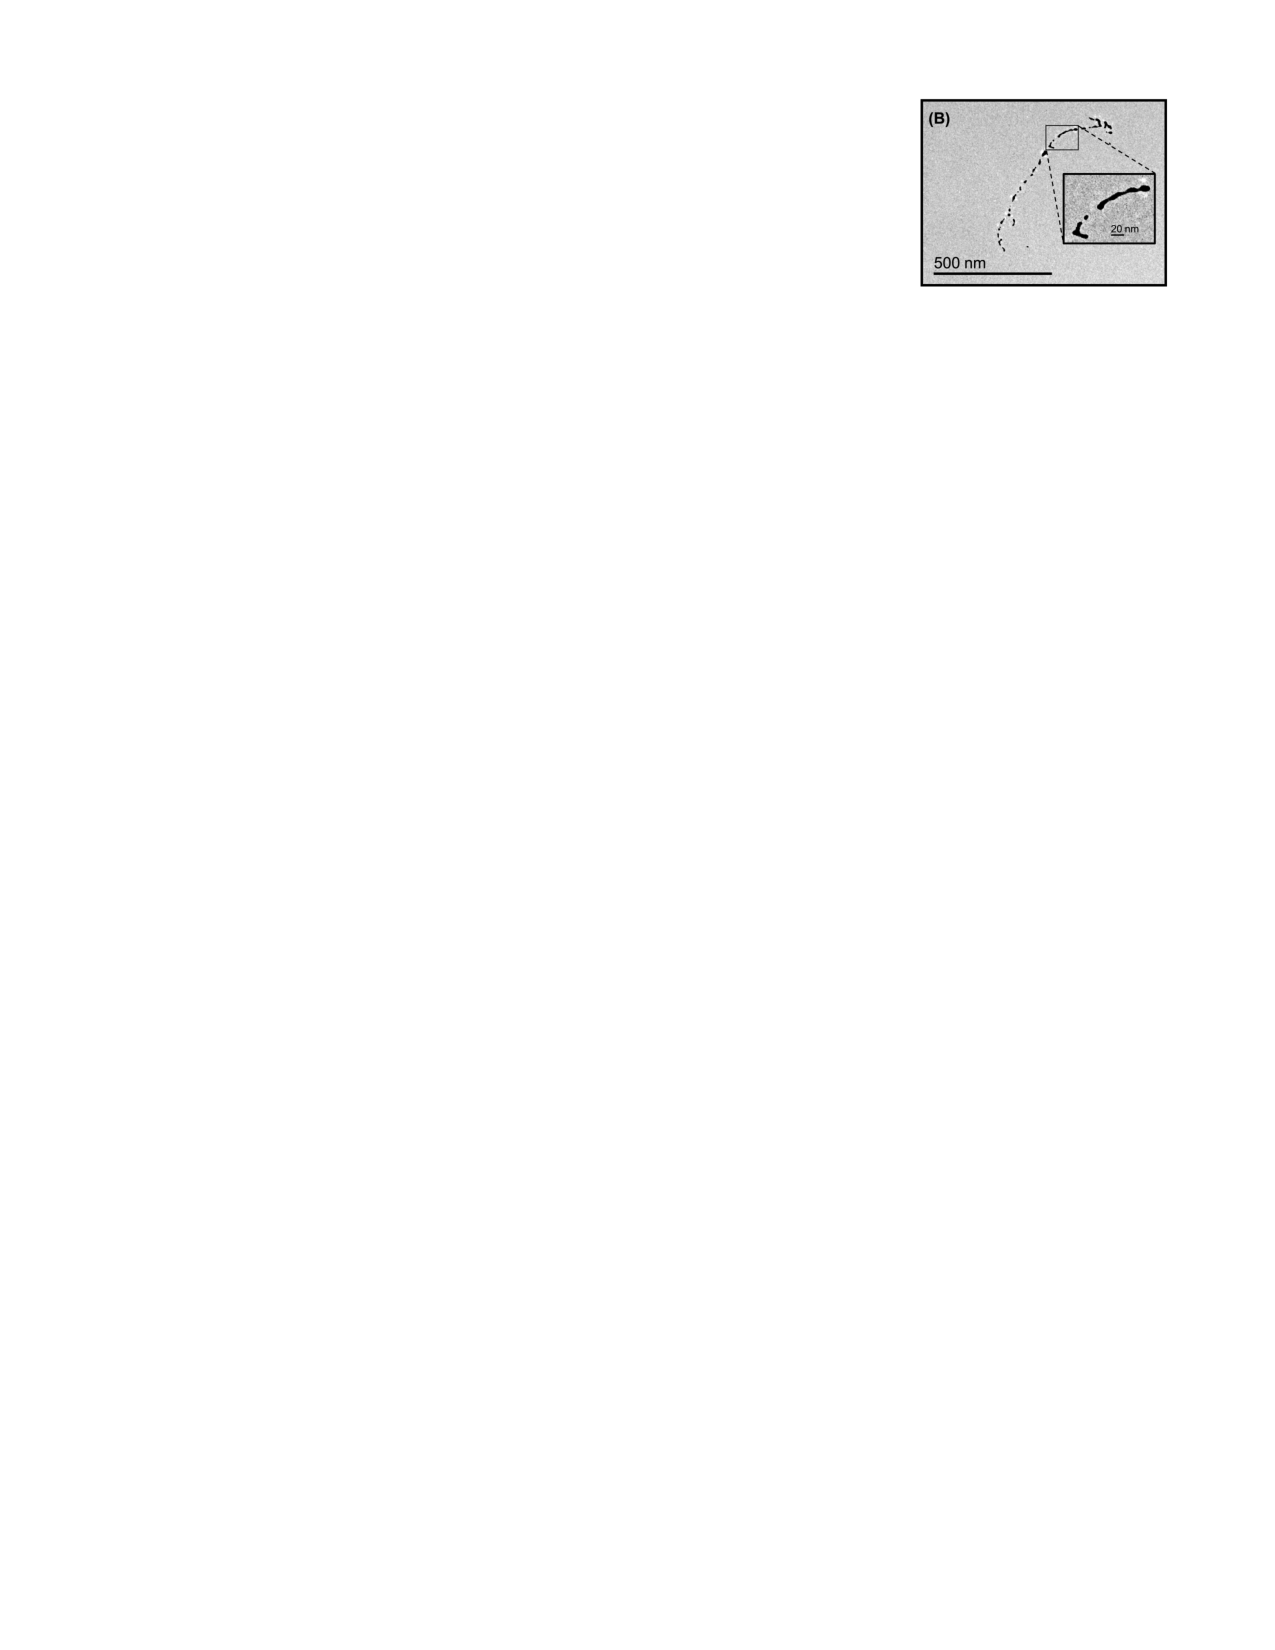
\includegraphics[width=0.75\textwidth]{silver-filament}
				\caption{Electron-microscope image of and elongated track-shaped Ag-cluster after it is surface-deposited.}
				\label{fig:silver-filament}
			\end{center}
		\end{figure}	
				
		\paragraph{Quantised vortices in He droplets} One of the most intriguing properties of superfluid helium droplets is the fact that they can host quantised vortices. Because of their ultra low temperature they are true quantum liquids and their vorticity and angular momentum are quantised. The existence of quantised vortices was anticipated because they have been created and observed in BECs made of dilute gases. However, the detection of quantised vortices is still experimentally challenging.
		
		\paragraph{The last few decades} A lot of of work has been done on helium droplets the last few decades, both experimentally and theoretically. From the absorption spectra of alkali metal doped helium droplets, the study of doped mixed $^3$He--$^4$He droplets, electrons in liquid helium, to the investigation of the critical Landau velocity inside small $^4$He droplet. For a comprehensive overview of work done in the last two decades, the interested reader is referred to the review papers[JLTP.Vol142.Nos.1/2(2006), IRPC.Vol36No4.621-707(2017), IRPC.Vol33No3.301-339(2014)].

%	\section{Structure of the thesis}
%		\lettrine[lines=3,findent=3pt,nindent=0pt]{T}{his} thesis will consist of two parts, since the presented work focusses on two distinct areas of interest with no mutual overlap. Each part will have its own short introduction to motivate the performed research and put in a broader context. The final chapter will conclude with some work in progress, planned work that has yet to start, and some ideas on how the method might be extended to be used in future research that is either cumbersome or impossible in its current form.
%
%		\subsection{Part I: Excited state dynamics}
%			In this part of the thesis the real-time dynamics of a single electronically excited rubidium (Rb) atom, residing in the surface dimple of a helium nano-droplet will be presented. The atom will be excited from its ground state 5s$^2\Sigma_{1/2}$ to the 5p$^2\{\Sigma,\Pi\}$ and 6p$^2\{\Sigma,\Pi\}$ manifold. This will be a combined experimental and theoretical study. The results are presented in two published articles:\\
%		
%			\emph{Imaging Excited-State Dynamics of Doped He Nanodroplets in Real-Time} will focus on imaging and characterising the dynamics using femtosecond spectroscopy and  time-dependent density functional theory.\\
%		
%			\emph{Desorption dynamics of RbHe-exciplexes off He nanodroplets induced by spin relaxation} is a combined experimental and theoretical investigation of the formation of free RbHe-exciplex molecules from laser-excited Rb-doped He nanodroplets through the mechanism of electronic spin relaxation. The role of relaxation of internal degrees of freedom of the RbHe exciplex in the desorption process has not been explicitly addressed.
%
%		\subsection{Part II: Collisions and capture by quantised vortices}
%			The second part investigates the real-time capture process of single xenon and argon atoms in their ground state by $^4$He$_{1000}$ droplets. Specifically it will address the interaction between a captured xenon or argon atom and a single quantised vortex line in the interior of the droplet. It will contain only theoretical investigations. The results will also be presented in two published works:\\
%		
%			\emph{Head-on Collisions of Xe Atoms Against Superfluid $^4\!$He Nanodroplets} studies the kinematics of head-on collisions between a xenon atom and a helium droplet. This scenario is then compared to a previous study of the same process with caesium to get a clear picture of the differences in dynamic behaviour between heliophilic and heliophobic species in said process. It also investigates different velocity regimes.\\
%		
%			\emph{Capture of Xe and Ar atoms by quantized vortices in $^4\!$He nanodroplets} addresses the capture of xenon and argon atoms at different velocity regimes and impact factors to determine the effective cross section for capture. This investigation then repeated with a dropet hosting one quantised line vortex. Also some preliminary results are presented for a larger droplet hosting an array of 6 line vortices, lined with argon atoms.
	\chapter{The DFT method for heavy impurities}\label{sec:dft-method}
	\epigraph{\flushright{One Functional to rule them all,\\
				One Functional to find them,\\
				One Functional to bring them all
				and in a droplet bind them.}}{\textit{F.M.G.J. Coppens}}

	\lettrine[lines=4,findent=3pt,nindent=0pt]{\color{activeColor}F}{rom} a theoretical point of view, superfluid helium must be considered as a high dimensional quantum system. Quantum Monte Carlo (QMC) \citep{Kro02} and direct quantum mechanical \citep{deL06,deL10,Agu13} calculations are the most accurate methods, but their computational demand quickly exceeds currently available computer resources when the number of helium atoms increases. Furthermore, QMC cannot describe dynamic evolution of superfluid helium in real time. To address these limitations, semi-empirical methods based on  density functional theory (DFT) formalism have been introduced\citep{Str87a,Str87b,Dal95}. DFT can be applied to much larger systems than QMC and allows for time-dependent formulation. As such, it offers a good compromise between accuracy and computational feasibility. The main drawback of DFT is that the exact energy functional is not known and must therefore be constructed in a semi-empirical manner. Moreover, doped helium droplets are limited to a mean-field description of the dopant-helium interaction. Nevertheless, DFT is the only method to date that can successfully reproduce results from a wide range of time-resolved experiments in superfluid helium, for realistic sizes compared to experimental conditions.
	
	\section{The Kohn-Sham approach}	\label{sec:kohn-sham}
		The starting point for the density functional method is the Hohenberg-Kohn (HK) theorem\citep{Hohenberg1964}, which states that the ground-state energy $E_v$ of an \emph{interacting inhomogeneous} system in a static potential $v$ can be written in as a unique functional of the one-body density $\rho$ as
		\begin{align}
			E_v[\rho] = \int\!v(\vec{r})\rho(\vec{r})\diff{r}+F[\rho] \label{eq1}
		\end{align}
		where $F[\rho]$ is a universal functional---valid for \emph{any} number of particles and \emph{any} external potential $v$---of the one-body density, defined as
		\begin{align}\label{eq:density-operator}
			\rho(\vec{r}) \vcentcolon= \ev**{\hat\rho(\vec{r})}{\Phi} = \ev**{\sum _{i=1}^{N}\delta(\vec{r}-\vec{r}_i)}{\Phi}
		\end{align}
		and $\Phi(\vec{r}_1,\vec{r}_2,\ldots,\vec{r}_N)$ is the many-body wave function of such a system. Furthermore, the functional $F[\rho]$ gives the ground state energy \emph{if and only if} the input density is the true ground state density of the system.
		
		Kohn and Sham (KS) later reformulated\citep{Kohn1965} the theory by introducing an approximation scheme for the functional $F[\rho]$ that is analogous to Hartree's method, but also contains the major part of the correlation effects inherent in interacting many-body systems. The approximation starts by defining
		\begin{align}
			F[\rho] \vcentcolon= T[\rho] + E_{c}[\rho]
		\end{align}
		where $T[\rho]$ is now the kinetic energy of a fictitious system of \emph{non-interacting} particles with density $\rho$ and $E_c[\rho]$ is the interaction term of an \emph{interacting} system with the same density, which contains all the other terms of the functional. For the kinetic part this allows us to write the total kinetic energy $T[\rho]$ as the sum of the individual kinetic energies $T_i$ of the non-interacting particles
		\begin{align}
			T = \sum_i T_i = -\frac{\hbar^2}{2m_4} \sum_i \ev**{\laplacian}{\varphi_i} = -\frac{\hbar^2}{2m} \sum_i \int\! \varphi_i^*({\mathbf r})\laplacian \varphi_i({\mathbf r})\diff{r}\,, \label{eq:kin-energy}
		\end{align}
		where $m_4$ is the mass of a $^4$He atom and the $\{\varphi_i\}$ are the Kohn-Sham single-particle orbitals corresponding to the many-body KS wave function $\Phi_{KS}(\vec{r}_1,\vec{r}_2,\ldots,\vec{r}_N)=\prod_i\varphi_i(\vec{r}_i)$ and leading to the density (using the definition in \eq{eq:density-operator}) $\rho(\vec{r})=\sum_i\absolutevalue{\varphi_i(\vec{r})}^2$.
	
		There is difference between the true kinetic energy of the interacting system and the fictitious one, due to the neglecting of the correlations. This difference is being corrected and accounted for in the correlation energy $E_c[\rho]$.
		
		Because the functional we used in this work is calibrated to produce the correct behaviour of bulk liquid helium at zero temperature $T=0$ and zero pressure $P=0$, we assume complete Bose-Einstein (BE) condensation of the helium. In this case all the helium atoms occupy the same single-particle KS-orbital $\varphi_0$. Therefore the many-body wave function and the density simplifies further to
		\begin{align}
			\Phi_{BEC}(\vec{r}_1,\vec{r}_2,\ldots,\vec{r}_N)=\prod_i\varphi_0(\vec{r}_i)
		\end{align}
		 and
		 \begin{align}
		 	\rho(\vec{r})=N\absolutevalue{\varphi_0(\vec{r})}^2
		 \end{align}
		 respectively. As explained in \scn{sec:bogol-order}, it is customary to define an effective wave function
		\begin{align}
			\Psi(\vec{r})\vcentcolon=\sqrt{\rho(\vec{r})}=\sqrt{N}\varphi_0(\vec{r}) \label{eq:order-param}	
		\end{align}
	 	for the condensate (see \eq{eq:order-param-real}), which is sometimes called a \emph{macroscopic wave function} or \emph{order parameter}. We can now simplify the expression for the kinetic energy (\eq{eq:kin-energy})
	%	\begin{align}
	%		T &= -\frac{\hbar^2}{2m} N \ev**{\laplacian}{\varphi_0} \nonumber \\
	%		  &= -\frac{\hbar^2}{2m} N\int\! \varphi_0^*(\vec{r})\laplacian \varphi_0(\vec{r})\diff{r} \nonumber \\
	%		 &= \frac{\hbar^2}{2m} N\int\! \abs{\grad{\varphi_0}}^2\diff{r} \label{eq5}
	%	\end{align}
		\begin{align}
			T = -\frac{\hbar^2}{2m_4} N\int\! \varphi_0^*(\vec{r})\laplacian \varphi_0(\vec{r})\diff{r}
			 = \frac{\hbar^2}{2m_4} N\int\! \abs{\grad{\varphi_0}}^2\diff{r}\,, \label{eq5}
		\end{align}	
		where we used partial integration to get to the last step and imposed that the orbital $\varphi_0$ vanishes at the boundaries. With our definition \eq{eq:order-param} we can now write the kinetic energy as a functional of the density
		\begin{align}
			T[\rho] = \frac{\hbar^2}{2m_4} \int\! \abs{\grad{\sqrt{\rho}}}^2\diff{r} 
		\end{align}
		To summarise, we write the complete energy functional $E_v$ as
		\begin{align}
			E_v[\rho] = \int\!v(\vec{r})\rho(\vec{r})\diff{r} + \frac{\hbar^2}{2m_4} \int\! \abs{\grad{\sqrt{\rho}}}^2\diff{r} + \int\!\mathcal{E}_c[\rho]\diff{r} \label{eq:ks-tot-energy}
		\end{align}
		where we defined the correlation energy density functional $\mathcal{E}_c$ through
		\begin{align}
			E_c[\rho] \vcentcolon= \int\!\mathcal{E}_c[\rho]\diff{r}\,.
		\end{align}
		The difficult job is to design a functional $\mathcal{E}_c$ such that the desired physical properties of helium can be recovered. This is far from trivial but several of these density functionals are available now. The one used in this work is discussed in \scn{sec:otdft}.
	
	\subsection{Time-dependent DFT}\label{sec:tddft}
	To describe the time evolution of the system, the Runge-Gross theorem extends DFT to its time-dependent version TDDFT\citep{Run84}. The functional variation of the associated action (see \eq{eq:action} for an example) leads to the following time-dependent Euler-Lagrange (EL) equation 
	\begin{align}
		i\hbar\frac{\partial}{\partial t} \Psi(\vec{r},t) = \left\{-\frac{\hbar^2}{2m_4}\laplacian + \fdv{\mathcal{E}_c}{\rho}\right\}\Psi(\vec{r},t) \vcentcolon= \mathcal{H}\qty[\rho]\Psi(\vec{r},t) 
		\label{eq:td-el-equation}
	\end{align}
	As long as we are in the thermodynamic regime the solutions $\Psi(\textbf{r},t)$ can be decomposed into the liquid density and associated velocity potential field (see \scn{sec:bogol-order} and \scn{sec:rot-vort}).
	
	Considering only eigenstates $\Psi(\vec{r},t)=\Psi_0(\vec{r})\unit{e}^{-i\mu t/\hbar}$ of the time independent Hamiltonian $\mathcal{H}\qty[\rho]$ the time-dependent EL-equation reduces to a time independent one
	\begin{align}
		\left\{-\frac{\hbar^2}{2m_4} \laplacian + \fdv{\mathcal{E}_c}{\rho}\right\}\Psi_0(\textbf{r}) = \mu\Psi_0(\textbf{r})
		\label{eq:el-equation}
	\end{align}
	with $\mu$ the chemical potential. Solving this equation by iteration will result in the ground state density $\abs{\Psi_0}^2$ of the system. Within the HK-framework and the variation principle that was used to obtain these EL-equations, the nature of the minimisation is such that it gives the lowest energy for a given symmetry. This means that as long as the input state does not break the symmetry of the time-independent EL-equation, it minimises the energy of this state even if it does not lead to the ground state. This can be used to obtain a stationary vortex-line solution. With the inclusion of appropriate constraints in the energy functional the same procedure can be used to obtain helium densities with an array of vortex-lines.

	\section{The Orsay-Trento Density Functional}\label{sec:otdft}
		\begin{table}
			\caption{Model parameters for the OT-DFT and solid functionals.}\label{tab:ot-params}
			\taburulecolor{activeColor}
			\begin{tabu} to \textwidth {X[c]X[c]X[c]X[2c]X[2c]X[c]}
				\toprule
				$\epsilon_{LJ}$~(K)	& $\sigma$~(\AA) & $h$~(\AA) & $c_2$~(K~\AA$^6$) & $c_3$~(K~\AA$^9$) & $\alpha_s$~(\AA$^3$) \\
				\midrule
				10.22 & 2.556 & 2.190323 & $-$2.41186~$\times~10^4$ & 1.85850~$\times~10^6$ & 54.31 \\
				&&&&& \\
				$\rho_{0s}$~(\AA$^{-3}$) & $l$~(\AA) & $C$~(Hartree) & $\beta$~(\AA$^3$) & $\rho_m$~(\AA$^{-3}$) & $\gamma_{11}$ \\
				\midrule
				0.04 & 1. & 0.1 & 40. & 0.37 & $-$19.7544 \\
				&&&&& \\
				$\gamma_{12}$~(\AA$^{-2}$) & $\alpha_1$~(\AA$^{-2}$) & $\gamma_{21}$ & $\gamma_{22}$~(\AA$^{-2}$) & $\alpha_2$~(\AA$^{-2}$) & \\ 
				\midrule
				12.5616 & 1.023 & $-$0.2395 & 0.0312 & 0.14912 & \\
				\bottomrule 
			\end{tabu}
		\end{table}

		\begin{figure}[t]
			\begin{center}
				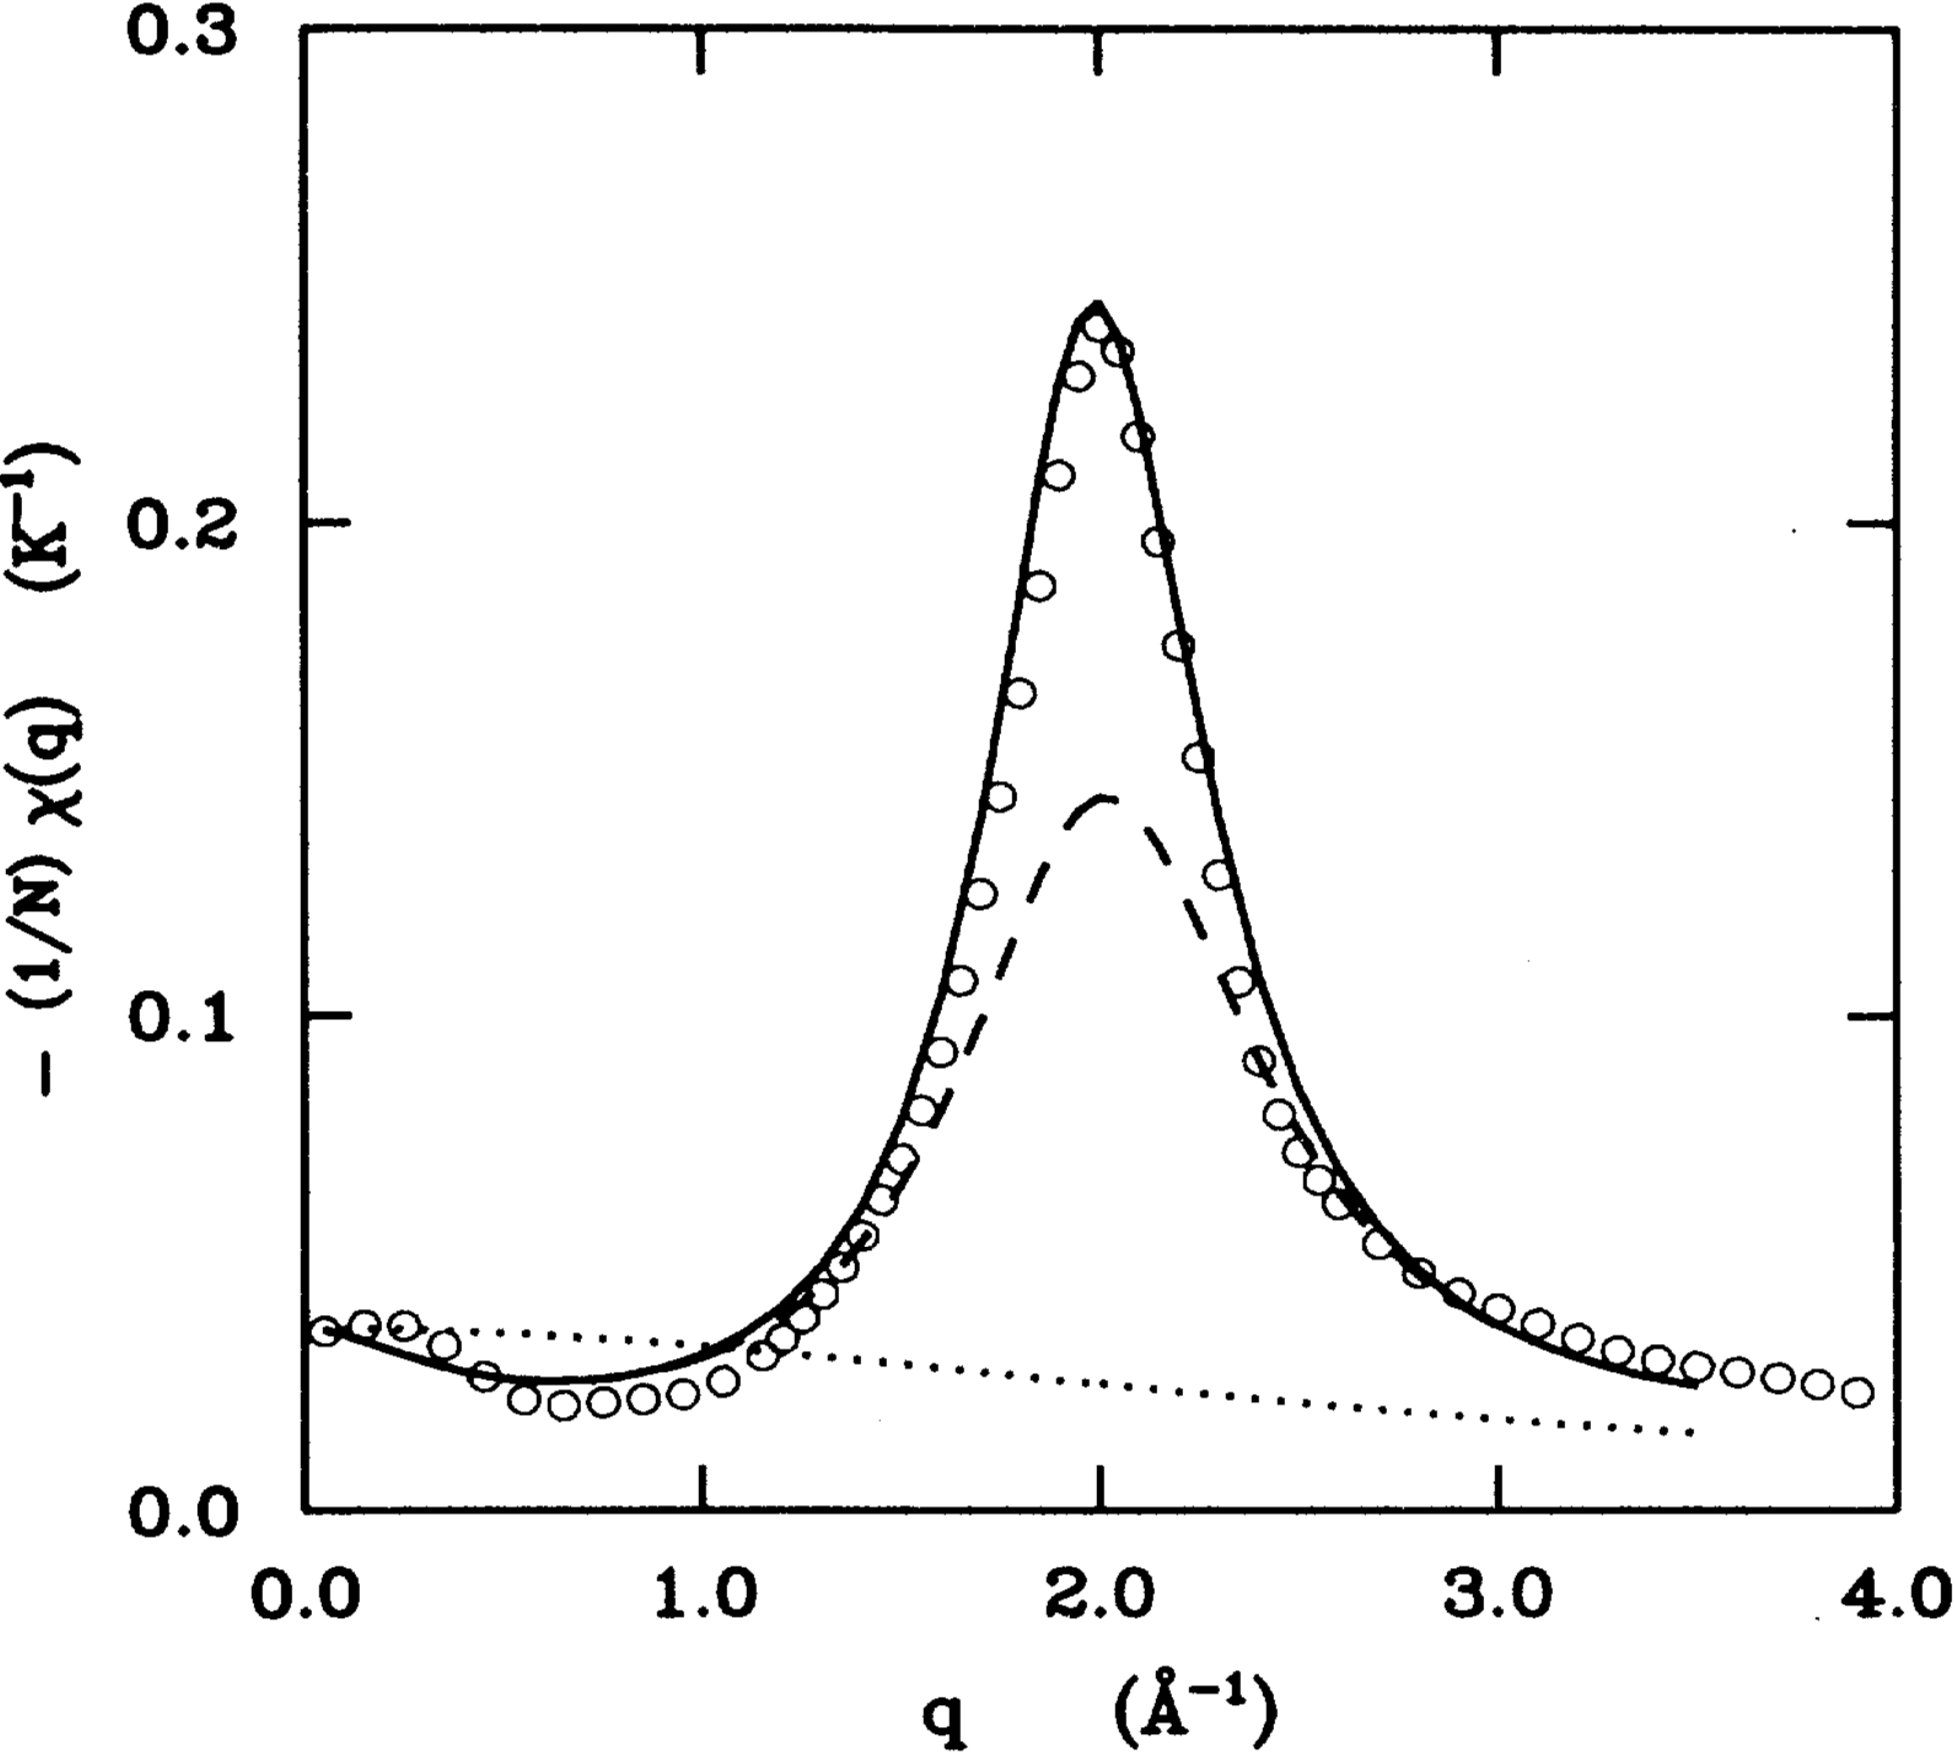
\includegraphics[width=0.75\textwidth]{static-response-function}
				\caption{Static response $-\chi$ (see\rf{Dalfovo1995}, Eqn.~(11)) per atom of liquid $^4$He at zero pressure. Points: experimental data; dotted line: from the functional of\rfs{Str87a,Str87b}; dashed line: Orsay-Paris (OP) functional\citep{Dupont-Roc1990}; solid line: OT functional.}
				\label{fig:static-response-function}
			\end{center}
		\end{figure}
	
		The functional that is used in the work presented in this thesis is based on the Orsay-Trento (OT) functional\citep{Dalfovo1995}. It uses a finite-range, non-local approach and it is, to date the most accurate model in the sense that its parameters were fitted to reproduce the bulk properties of liquid helium at $T=0=P$. It is written as
		\begin{align}
			\mathcal{E}_c[\rho ,\vec{v}] &=  
			\frac{1}{2} \left.\int \! \right\{\rho({\bf r}) V_{LJ}(|{\bf r}-{\bf r'}|) \rho({\bf r'}) \nonumber \\
			&+ \left.\frac{1}{2} c_2\, \rho({\bf r}) \left[{\bar \rho}({\bf r}) \right]^2 
			+ \frac{1}{3} c_3 \, \rho({\bf r}) \left[ {\bar \rho}({\bf r}) \right]^3\right\}\diff{r'} \nonumber \\
			&- \frac{\hbar^2}{4m_4} \alpha_s \int \! F(|{\bf r}-{\bf r'}|) \left[ 1- \frac{{\tilde \rho}({\bf r})}{\rho_{0s}} \right]\grad{\rho({\bf r})} \cdot \grad{\rho({\bf r'})} \left[ 1- \frac{{\tilde \rho}({\bf r'})}{\rho_{0s}} \right]\diff{r'} \nonumber \\
			& - \frac{m_4}{4} \int \! V_J(| \mathbf{r} - \mathbf{r}'|)\, \rho(\mathbf{r}) \, \rho(\mathbf{r}')\,  [\mathbf{v}(\mathbf{r})-\mathbf{v}(\mathbf{r}')]^2\diff{r'} \label{eq:otf}
		\end{align}
		The first term corresponds to a classical Lennard-Jones type two-body interaction between helium atoms. The interaction is screened at short distances where the interaction energy is of the same order as the correlation effects:
		\begin{align}
			V_{LJ}(r) = \begin{cases}
			\epsilon_{LJ} \left[\left(\frac{\sigma}{r} \right)^{12} - \left(\frac{\sigma}{r} \right)^{6} \right] & {\rm if} \quad r > h \\
			0 & {\rm otherwise}
			\end{cases}\label{eq9}
		\end{align}
		In the second line, the terms corresponding to $c_2$ and $c_3$, correct for short range correlations when $r<h$. The weighted density $\bar{\rho}$ is the average density $\rho$ over a sphere of radius $h$:
		\begin{align}
			\bar{\rho}(\vec{r}) = \int\!\Pi_h\qty(\abs{\vec{r}-\vec{r'}})\rho({\vec{r'}})\diff{r'},
		\end{align}
		with
		\begin{align}
			\Pi_h(r) \vcentcolon= \begin{cases}
				\frac{3}{4\pi h^3} & \rm{if} \quad r\leq h \\
				0 & \rm{otherwise}
			\end{cases}
		\end{align}
		The third line is a non-local correction to the kinetic energy (KC). It partially accounts for the difference $\mathcal{T}[\rho]-T[\rho]$ mentioned in \scn{sec:kohn-sham}. The gradient-gradient interaction function $F$ is a Gaussian kernel defined as
		\begin{align}
			F(r) = \frac{1}{l^3\sqrt{\pi^3}}\unit{e}^{-r^2/l^2}
		\end{align}
		All the parameters are fitted to reproduce the peak of the static response function (see \fig{fig:static-response-function}) in the bulk liquid. The factor $\qty(1-\tilde{\rho}/\rho_{0s})$ is included to match the pressure dependence of the static response function predicted by diffusion Monte Carlo calculations\citep{Moroni1992}. The quantity $\tilde{\rho}(\vec{r})$ is another weighted density, calculated using $F$ as a weight
		\begin{align}
			\tilde{\rho}(\vec{r}) \vcentcolon= \int\!F\qty(\abs{\vec{r}-\vec{r'}})\rho(\vec{r'})\diff{r'}
		\end{align}
		The density $\tilde{\rho}(\vec{r})$ is very close to the normal density $\rho(\vec{r})$ except in very inhomogeneous situations. For pure helium droplets and free helium surfaces one can safely use $\rho$ instead of $\tilde{\rho}$. In the presence of significant short-range density oscillations, e.g. in the presence of heavy atomic impurities as presented in this thesis or electrons, the helium density needs to be smoothed by the Gaussian kernel $F$.  
			
		Finally, the last line in \eq{eq:otf} is called the \emph{back-flow} term and influences the dynamic response of the system. It plays the role of a non-local kinetic energy. Since the back-flow contains the factor $\vec{v}-\vec{v'}$, with $\vec{v}$ defined in \eq{eq:velocity-field}, the contribution will only be non-zero whenever the effective wave function $\Psi$ is complex-valued. Consequently, for time-independent cases it means that this will only affect the vortex states. The phenomenological effective current-current interaction $V_J(r)$ is calibrated so that it reproduces the experimental phonon-roton spectrum (see \fig{fig:dispersion-relation}):
		\begin{align}
			V_J(r) =\,&(\gamma_{11} +\gamma_{12} \, r^2) e^{-\alpha_1 r^2} \nonumber \\
				+\,&(\gamma_{21} +\gamma_{22} \, r^2) e^{-\alpha_2 r^2}
		\end{align}
		All the parameters of the functional are given in \tab{tab:ot-params}.

		\subsection{The Solid-OT Density Functional}
			In the presence of highly inhomogeneous liquid densities, e.g. atomic impurities with a very strong He-X interaction, the OT-functional \eq{eq:otf} becomes numerically unstable. To deal with this problem an additional cut-off can be used
			\begin{align}
				\mathcal{E}^\mathrm{sol} \vcentcolon= C\rho(\vec{r})\qty{1+\tanh(\beta\qty[\rho(\vec{r})-\rho_\mathrm{m}])}
			\end{align}
			where the model parameters $\qty{C,\beta,\rho_\mathrm{m}}$ are specified in \tab{tab:ot-params}. Including this term in the OT-functional prevents excessive density build-up. $\mathcal{E}^\mathrm{sol}$ only starts to deviate from zero whenever the liquid density $\rho$ is comparable to $\rho_\mathrm{m}$ or larger. Therefore, inclusion of this term in the functional does not alter the density distribution. This penalty term was originally developed to account for the liquid-solid phase transition of $^4$He\citep{Anc05a,Cau07}. The functional that has been used to obtain the result presented in this work is refered to as the ``Solid-OT-DFT functional''. It consists of the first three terms of the original OT-functional \eq{eq:otf}, plus $\mathcal{E}^\mathrm{sol}$
			\begin{align}
				\mathcal{E}_c^\mathrm{sol}[\rho] &=  
				\frac{1}{2} \left.\int \! \right\{\rho(\vec{r}) V_{LJ}(\abs{\vec{r}-\vec{r'}}) \rho(\vec{r'}) \nonumber \\
				&+ \left.\frac{1}{2} c_2\, \rho(\vec{r}) \qty[\bar\rho(\vec{r})]^2 
				+ \frac{1}{3} c_3 \, \rho(\vec{r}) \qty[\bar\rho(\vec{r})]^3\right\}\diff{r'} \nonumber \\
				&+ C\,\rho(\vec{r})\qty\Big{1+\tanh(\beta\qty[\rho(\vec{r})-\rho_\mathrm{m}])} \label{eq:solid-otf}
			\end{align}

	\section{Static calculations}
		In the work presented here all the impurities are heavy compared to the mass of $^4$He, e.g. the mass of rubidium (Rb) is about 21 times larger than that of helium (He), xenon (Xe) roughly 33 times and argon (Ar) about 10 times. Therefore we are allowed to treat the centre of mass motion of the impurities as classical. It was also checked for potassium (K) which is slightly lighter than Ar\citep{Martinez2017}. In the functional this will be modelled as an external field $V_X$, the impurity-He pair interaction
		\begin{align}
			E[\rho] \rightarrow E[\rho] + \!\int\!\rho(\vec{r})\,V_X\qty(\abs{\vec{r}-\vec{r}_I})\diff{r} \label{eq:el-static-hi}
		\end{align}
		where ${\vec r}_I$ is the location of the impurity. Varying the modified functional to minimise the energy one now finds a new EL-equation in which the helium--impurity interaction is included:
		\begin{align}
			\left\{-\frac{\hbar^2}{2m_4} \laplacian + \fdv{\mathcal{E}_c}{\rho} + V_X(|{\mathbf r} - {\mathbf r_I}|)\right\}\Psi({\mathbf r}) = \mu \Psi({\mathbf r}) \label{eq:el-static-hi}
		\end{align}
		This equation is then solved by iteration in a self-consistent way by the imaginary time propagation method\citep{Lehtovaara2007} (ITM) in cartesian coordinates. The calculations are performed in three dimensions without imposing any symmetries that are present in the external potential. All the quantities are discretised on an evenly spaced Cartesian grid with a step-size that is typically of the order of 0.4~\AA. The differential operators are evaluated using a $k$-point finite difference method where in most applications $k=13$ is sufficiently accurate. The integrals in the density-functional can be expressed as convolutions and can therefore be evaluated in momentum-space by exploiting the convolution theorem, using proprietary highly optimised parallel Fast Fourier Transform algorithms. 
			
		\subsection{Producing vortical states}\label{sec:vortical-states}
			The helium density that minimises the energy of the vortical states $\Psi_s$ (\eq{eq:line-vortex}), introduced in \scn{sec:rot-vort}, can be obtained by solving the same EL-equation as for a vortex-free droplet. This becomes clearer when we write \eq{eq:el-equation} in cylindrical coordinates:
			\begin{align}
				\qty{-\frac{\hbar^2}{2m_4}\qty[\frac{1}{r}\pdv{r}\qty(r\pdv{r})-\frac{s^2}{r^2}]+\fdv{\mathcal{E}_c}{\rho}}\Psi_s(\vec{r}) = \mu\Psi_s(\vec{r}) \label{eq:el-cyl}
			\end{align}
			Written like this it is evident that the ground state $\Psi_0$ is just the special case for $s=0$. Obtaining the solution using the ITM works as long as the solution has overlap with initial guess for the order parameter. Starting with a trial order parameter similar to $\Psi_s$ will guarantee this. To do this we apply the ``imprinting'' technique where we apply the ground state density of a previously obtained vortex-free droplet and multiply it with a normalised complex factor
			\begin{align}
				\Psi(\mathbf{r}) = \sqrt{\rho_0(\vec{r})} \,\times \frac{x + iy}{\sqrt{x^2 + y^2}} \label{eq28}
			\end{align}
			where $\rho_0$ is the ground state density of the vortex-droplet.  In cylindrical coordinates this factor is equivalent to the one in \eq{eq:line-vortex} for $s=1$. 
			
			This changes for droplets with two or more vortices, where the cylindrical symmetry is broken and the solutions are no longer solutions of \eq{eq:el-cyl}, nor eigenfunctions of the angular momentum operator. In this case the time-independent EL-equation has to be modified to include a rotational constraint solution in the co-rotating frame
			\begin{align}
				{\cal H} \rightarrow {\cal H}-\Omega \hat{L}_z
			\end{align}
			 such that for a suitable choice of $\Omega$ the vortex-array solution becomes favourable to the ground state and also to excited states with angular momentum $s\geq 2$. Since these states are no longer eigenstates of the original time-dependent Hamiltonian, these states are no longer stationary and will start to rotate with frequency $\Omega$. The initial guess for a droplet with $n_v$ vortices can be produced using the same imprinting method as mentioned before		
			\begin{align}
				\Psi(\mathbf{r})=\sqrt{\rho_0(\vec{r})} \times \prod _{j=1}^{n_v}\left[ {(x-x_j)+i(y-y_j) \over \sqrt{(x-x_j)^2+(y-y_j)^2}}  \right] \label{eq32}
			\end{align}
			where $\rho_0$ is again the ground state density of the vortex-free droplet and $(x_j,y_j)$ is the initial position of the $j$-th vortex-line parallel to the $z$-axis.

	\section{Dynamic calculations}\label{sec:td-dft}
		For the dynamic evolution of atomic impurities excited from $n$s-states to $n'$s-states, we do not need to keep track of the evolution of the electronic state of the impurity since it keeps its spherically symmetric orbital. In this case we only need to describe the time evolution of the centre of mass coordinate of the impurity. As in the statics, because of the large atomic mass of the impurity compared to helium, the time evolution of the centre of mass coordinate of the impurity is treated classically. To obtain the correct energy for the whole droplet-impurity system the energy functional needs to be extended to include the impurities centre of mass motion and the impurity-helium interaction
		\begin{align}
			E[\rho] \rightarrow E[\rho] + \frac{p^2_I}{2 m_I} + \int \! \rho(\mathbf{r}) \, V_{X^{\!*}}\qty(\abs{\vec{r}-\vec{r}_I})\diff{r} \label{eq33}
		\end{align}
		where $p_I$ is the classical momentum of the impurity (which was not present in the static case, \eq{eq:el-static-hi}), $m_I$ is the impurity mass and $V_{X^{\!*}}$ is the impurity-He pair interaction potential for an impurity in the ground-, excited $n'$s- or ionised state. The equations of motion for the time evolution of the effective wave function $\Psi\qty(\vec{r},t)$ and the second time derivative of the impurity location $\ddot{\vec{r}}_I$ are  
		\begin{align}
			i\hbar\frac{\partial}{\partial t} \Psi &= \qty[-\frac{\hbar^2}{2m_4} \laplacian +\frac{\delta {\cal E}_c}{\delta \rho} + V_{X^*}(|\mathbf{r}- \mathbf{r}_I|)]\Psi\nonumber\\
			m_I \ddot{\mathbf{r}}_I &= - \grad_{\vec{r}_I} \left[  \int \!\rho(\mathbf{r}) V_{X^*}(|\mathbf{r}- \mathbf{r}_I|)\diff{r}  \right] \nonumber \\
			&= -\int \! V_{X^*}(|\mathbf{r}- \mathbf{r}_I|)  \, \grad \rho(\mathbf{r})\diff{r} \label{eq34}
		\end{align}
	
		\subsection{Diatomics in Molecules}\label{sec:dim-model}
			\begin{figure}[t]
				\begin{center}
					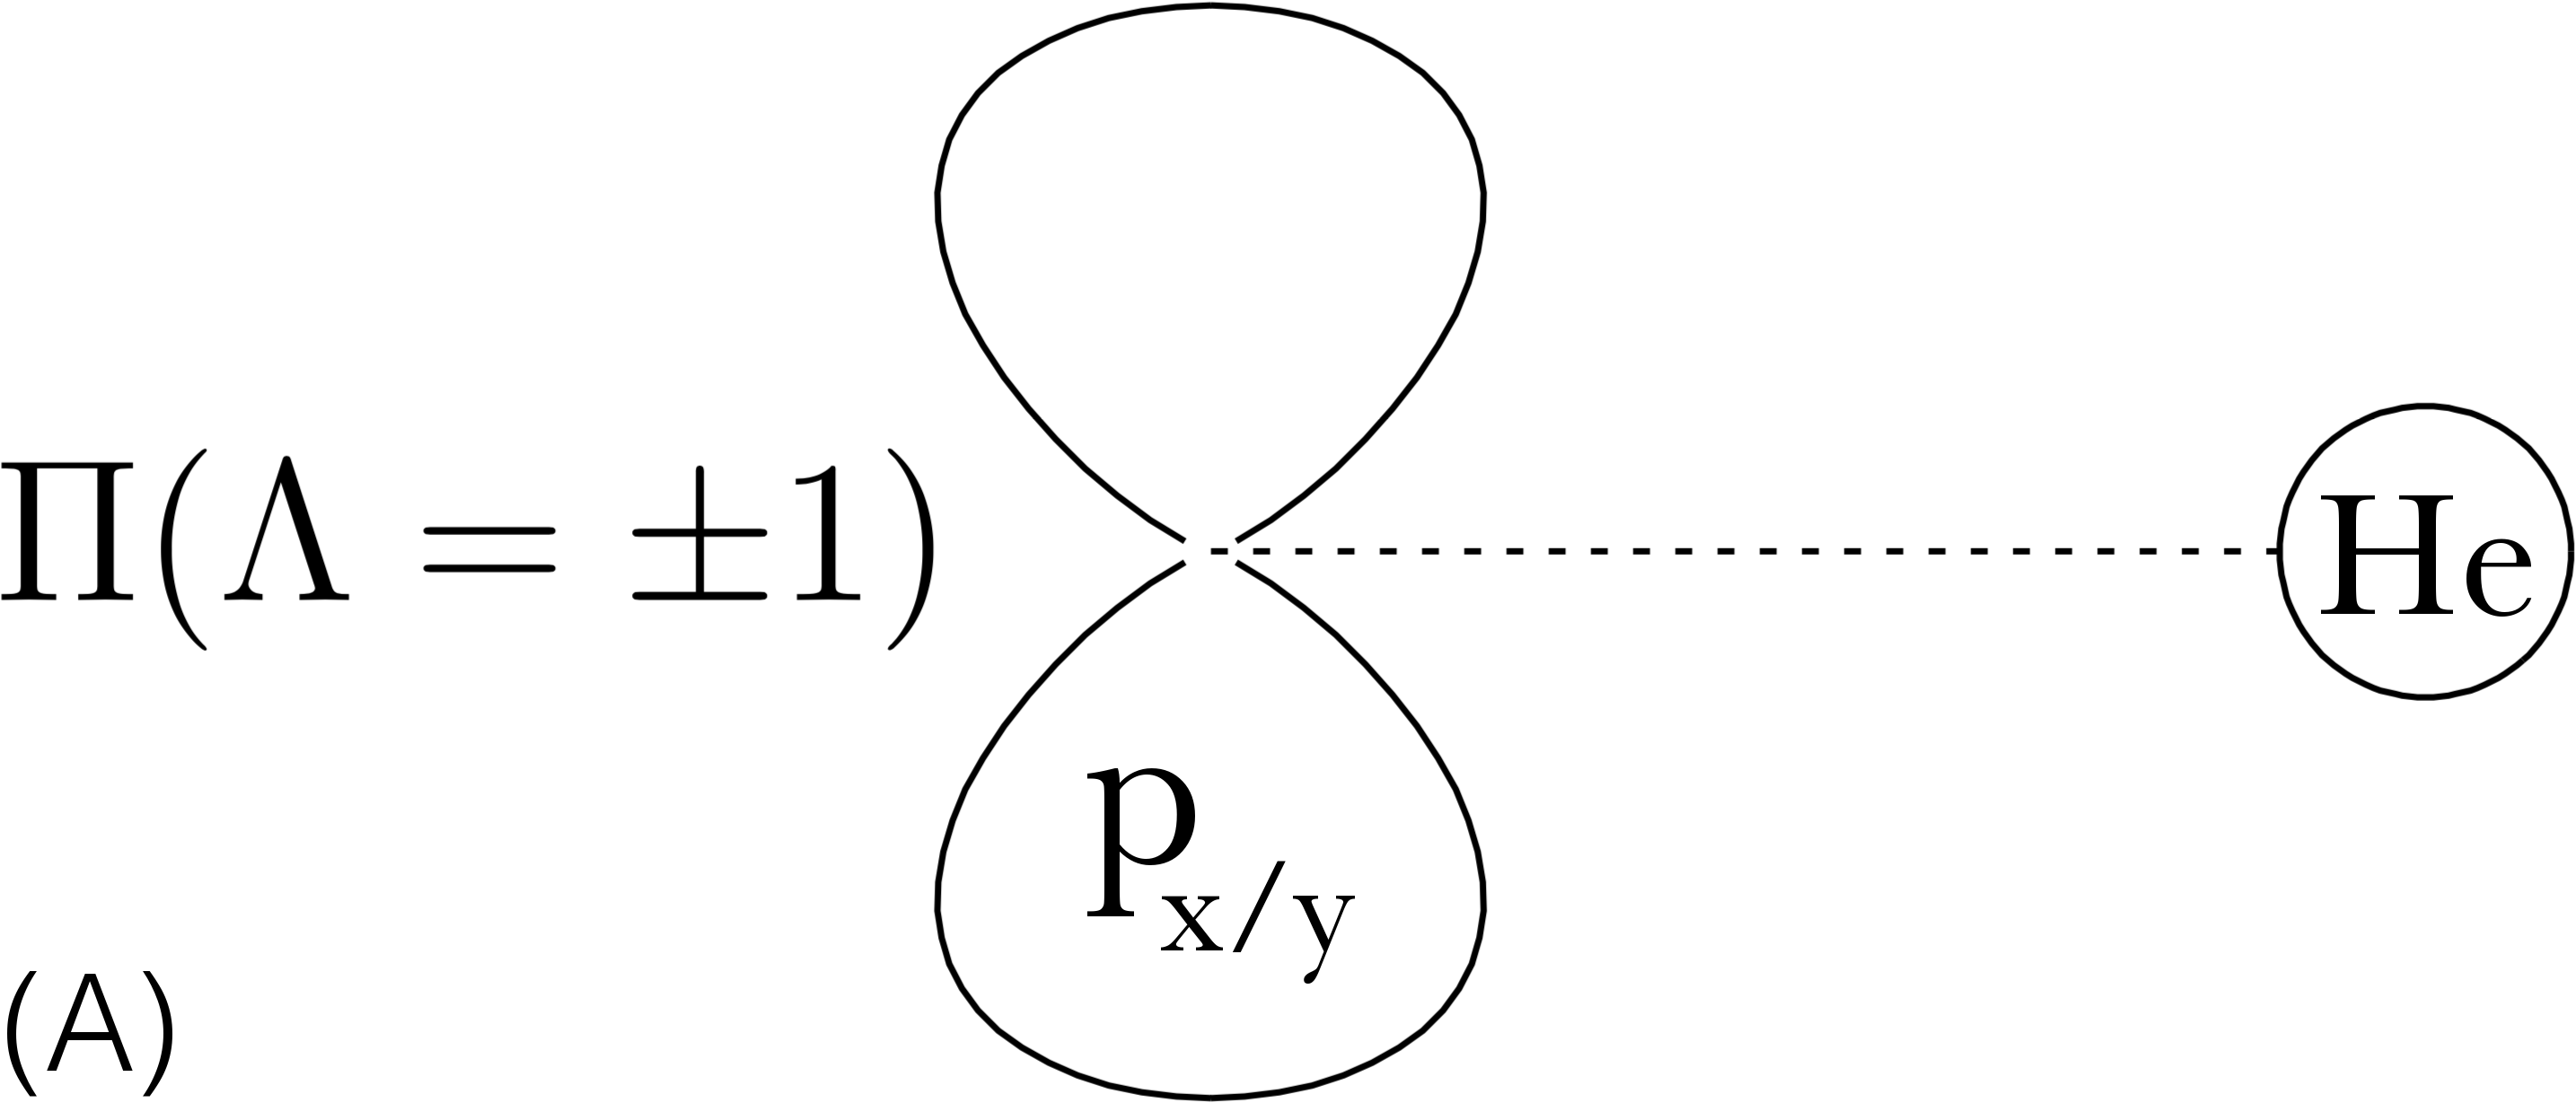
\includegraphics[width=0.45\textwidth]{pxy-he}
					\hspace{20pt}
					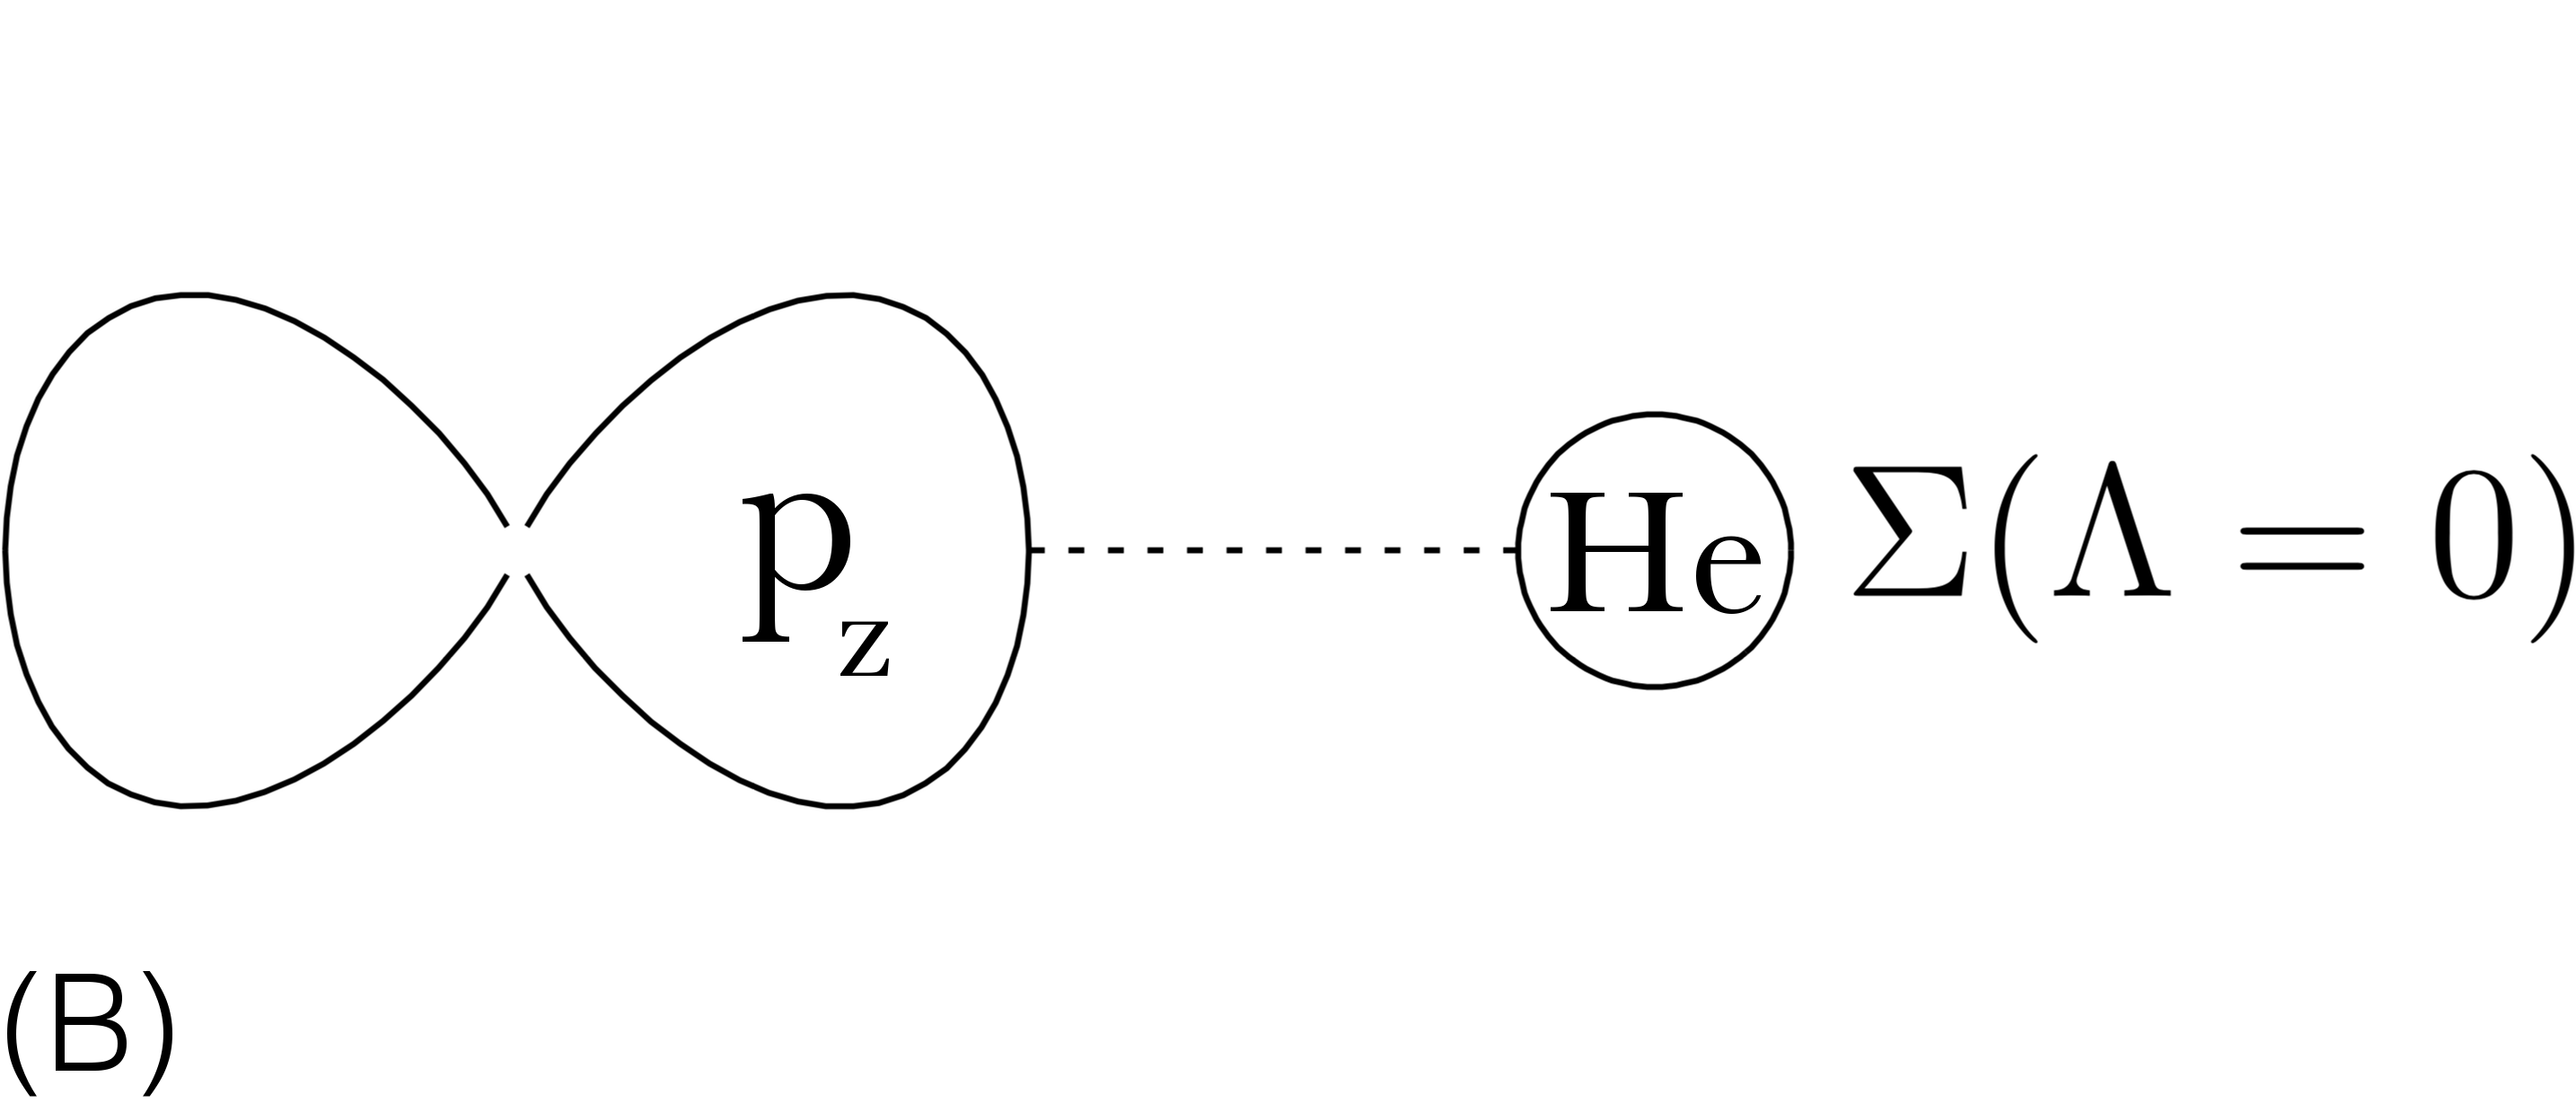
\includegraphics[width=0.45\textwidth]{pz-he}
				\end{center}
				\caption{Level splitting of the p-orbitals in the presence of helium, that breaks the spherical symmetry. (A)~A double degenerate n'p$_\mathrm{x/y}$-orbital and (B)~a single n'p$_\mathrm{z}$-orbital. (Illustration courtesy of M. Martinez\citep{Martinez2017}.)}
				\label{fig:p-orbitals}
			\end{figure}				
			The situation becomes slightly more complicated for $n$s-states excited to $n'$p-states (effective one-electron excited $^2$P-states). Since the three p-orbitals are no longer spherically symmetric and start mixing due to the interaction with the He droplet and spin-orbit coupling, we also need to include a description that accounts for the mixing of these orbitals in a dynamic way. To do this we use Diatomics in Molecules\citep{Ellison1963}(DIM). The interaction between a helium atom ($^1$S$_0$-state) and the triply degenerate $L=1$ electronic state of the impurity partially lifts the degeneracy so that the interaction can be decomposed into a $\Sigma$-state and a doubly degenerate $\Pi$-state (see \fig{fig:p-orbitals}). In the cylindrical symmetry it is customary to use the molecular term symbol $^{2S+1}\Lambda_\Omega$ to label the levels. In the bound region of the potentials $S$ is the electronic spin angular momentum (and $2S+1$ the spin multiplicity), $\Lambda$ is the quantum number for the projection of the electronic orbital angular momentum and $\Omega$ is the total electronic angular momentum, along the internuclear axis. Or symbolically
			\begin{align}
				m_j=m_l+m_s\:\longrightarrow\:\Omega=\Lambda+m_s
			\end{align}
			 Following the spectroscopic notation the orbitals corresponding to $\Lambda=0,1,2,3,\ldots$ are labeled $\Sigma,\Pi,\Delta,\Phi,\ldots$. The state vector of the impurity interacting with a He atom can be expressed in an uncoupled basis
			\begin{align}
				 \ket{p_{im}}\in\qty\big{\,\ket{p_{xm}}\!,\ket{p_{ym}}\!,\ket{p_{zm}}} \label{eq:dim-basis}
			\end{align}
			of real one-electron p-orbitals oriented along the internuclear axis (see \fig{fig:dim-axes}). The helium-impurity interaction matrix is given by
			\begin{align}
				\mathcal{V}^{DIM}(r_m) &= V_{\Pi}(r_m)\qty\big(\dyad{p_{xm}}+\dyad{p_{ym}})+V_{\Sigma}(r_m)\dyad{p_{zm}} \nonumber \\
					&= V_{\Pi}(r_m)\qty\big(\mathbb{1}_3-\dyad{p_{zm}})+V_{\Sigma}(r_m)\dyad{p_{zm}} \nonumber \\
					&=V_{\Pi}(r_m)\mathbb{1}_3+\qty\big[V_{\Sigma}(r_m)-V_{\Pi}(r_m)]\dyad{p_{zm}}
			\end{align}	
			where $r_m$ is the modulus of the interatomic separation vector and $V_\Pi$ and $V_\Sigma$ are the $\Pi$ and $\Sigma$ impurity-He pair potentials in the absence of spin-orbit coupling. For a system consisting of $N$ helium atoms the total interaction energy is calculated by summing over all the contributions of the $N$ individual $^4$He--X contributions
			\begin{align}
				\mathcal{U}^{DIM}(\vec{r}_I)=\sum_{m=1}^{N}\mathcal{V}^{DIM}(r_m)
			\end{align}
			It is more convenient to express the interaction in a basis common to all impurity-helium pairs, instead of a basis that depends on the particular impurity-helium pair chosen. To do this we apply a rotation $\mathcal{R}_m:\hat{\vec{z}}_m\mapsto\hat{\vec{z}}\propto\vec{r}_I$, so that the matrix corresponding to the $m^{\rm th}$ $^4$He atom expressed in the common basis is given by
			\begin{align}
				\dyad{p_{zm}} = \mathcal{R}_m\dyad{p_z}\mathcal{R}_m^{-1}
			\end{align}
			It can be shown that the elements of this matrix in cartesian coordinates are of the form
			\begin{equation}
				\mel**{p_i}{\mathcal{R}_m\dyad{p_z}\mathcal{R}_m^{-1}}{p_j} = \frac{r_{im}\,r_{jm}}{\norm{\vec{r}_m}^2}		\label{eq39}
			\end{equation}	
			where $(i,j)\in\qty{x,y,z}$. With these definitions we can write the matrix elements $U^{DIM}_{ij}$ of the interaction energy $\mathcal{U}^{DIM}$
			\begin{align}
				U^{DIM}_{ij}(\vec{r}_I)=\mel**{p_i}{\mathcal{U}^{DIM}}{p_j} = \sum_{m=1}^{N} V^{DIM}_{ij}(r_m)
			\end{align}
			where
			\begin{align}
				V^{DIM}_{ij}(r_m) \vcentcolon= V_\Pi(r_m)\delta_{ij}+\qty\Big[V_\Sigma(r_m)-V_\Pi(r_m)]\frac{r_{im}\,r_{jm}}{\norm{\vec{r}_m}^2} \label{eq:vdim}
			\end{align}
			are the matrix elements of $\mathcal{V}^{DIM}$ expressed in the common basis. Since we are working with a continuous helium density $\rho(\vec{r})$ and not with discrete atoms, the summation over $N$ helium atoms in the previous expression is replaced by an integral over the density $\sum_m\rightarrow\int\!\rho(\vec{r})\diff{r}$. Here we dropped the subscript $m$, representing the $m^\mathrm{th}$ helium atom. This finally gives for the matrix element $U^{DIM}_{ij}$
			\begin{align}
				U^{DIM}_{ij}(\vec{r}_I) = \int\! \rho\qty(\vec{r}+\vec{r}_I)\,V^{DIM}_{ij}(r)\diff{r} \label{eq:u-dim}
			\end{align}
			
			The eigenvalues $U^{\mathrm{np}}_k(\vec{r}_I)$ of this real symmetric matrix define the potential energy curves (PECs) without spin-orbit coupling as a function of the distance between the surrounding helium and the impurity for a given helium density.
			\begin{figure}[t]
				\begin{center}
					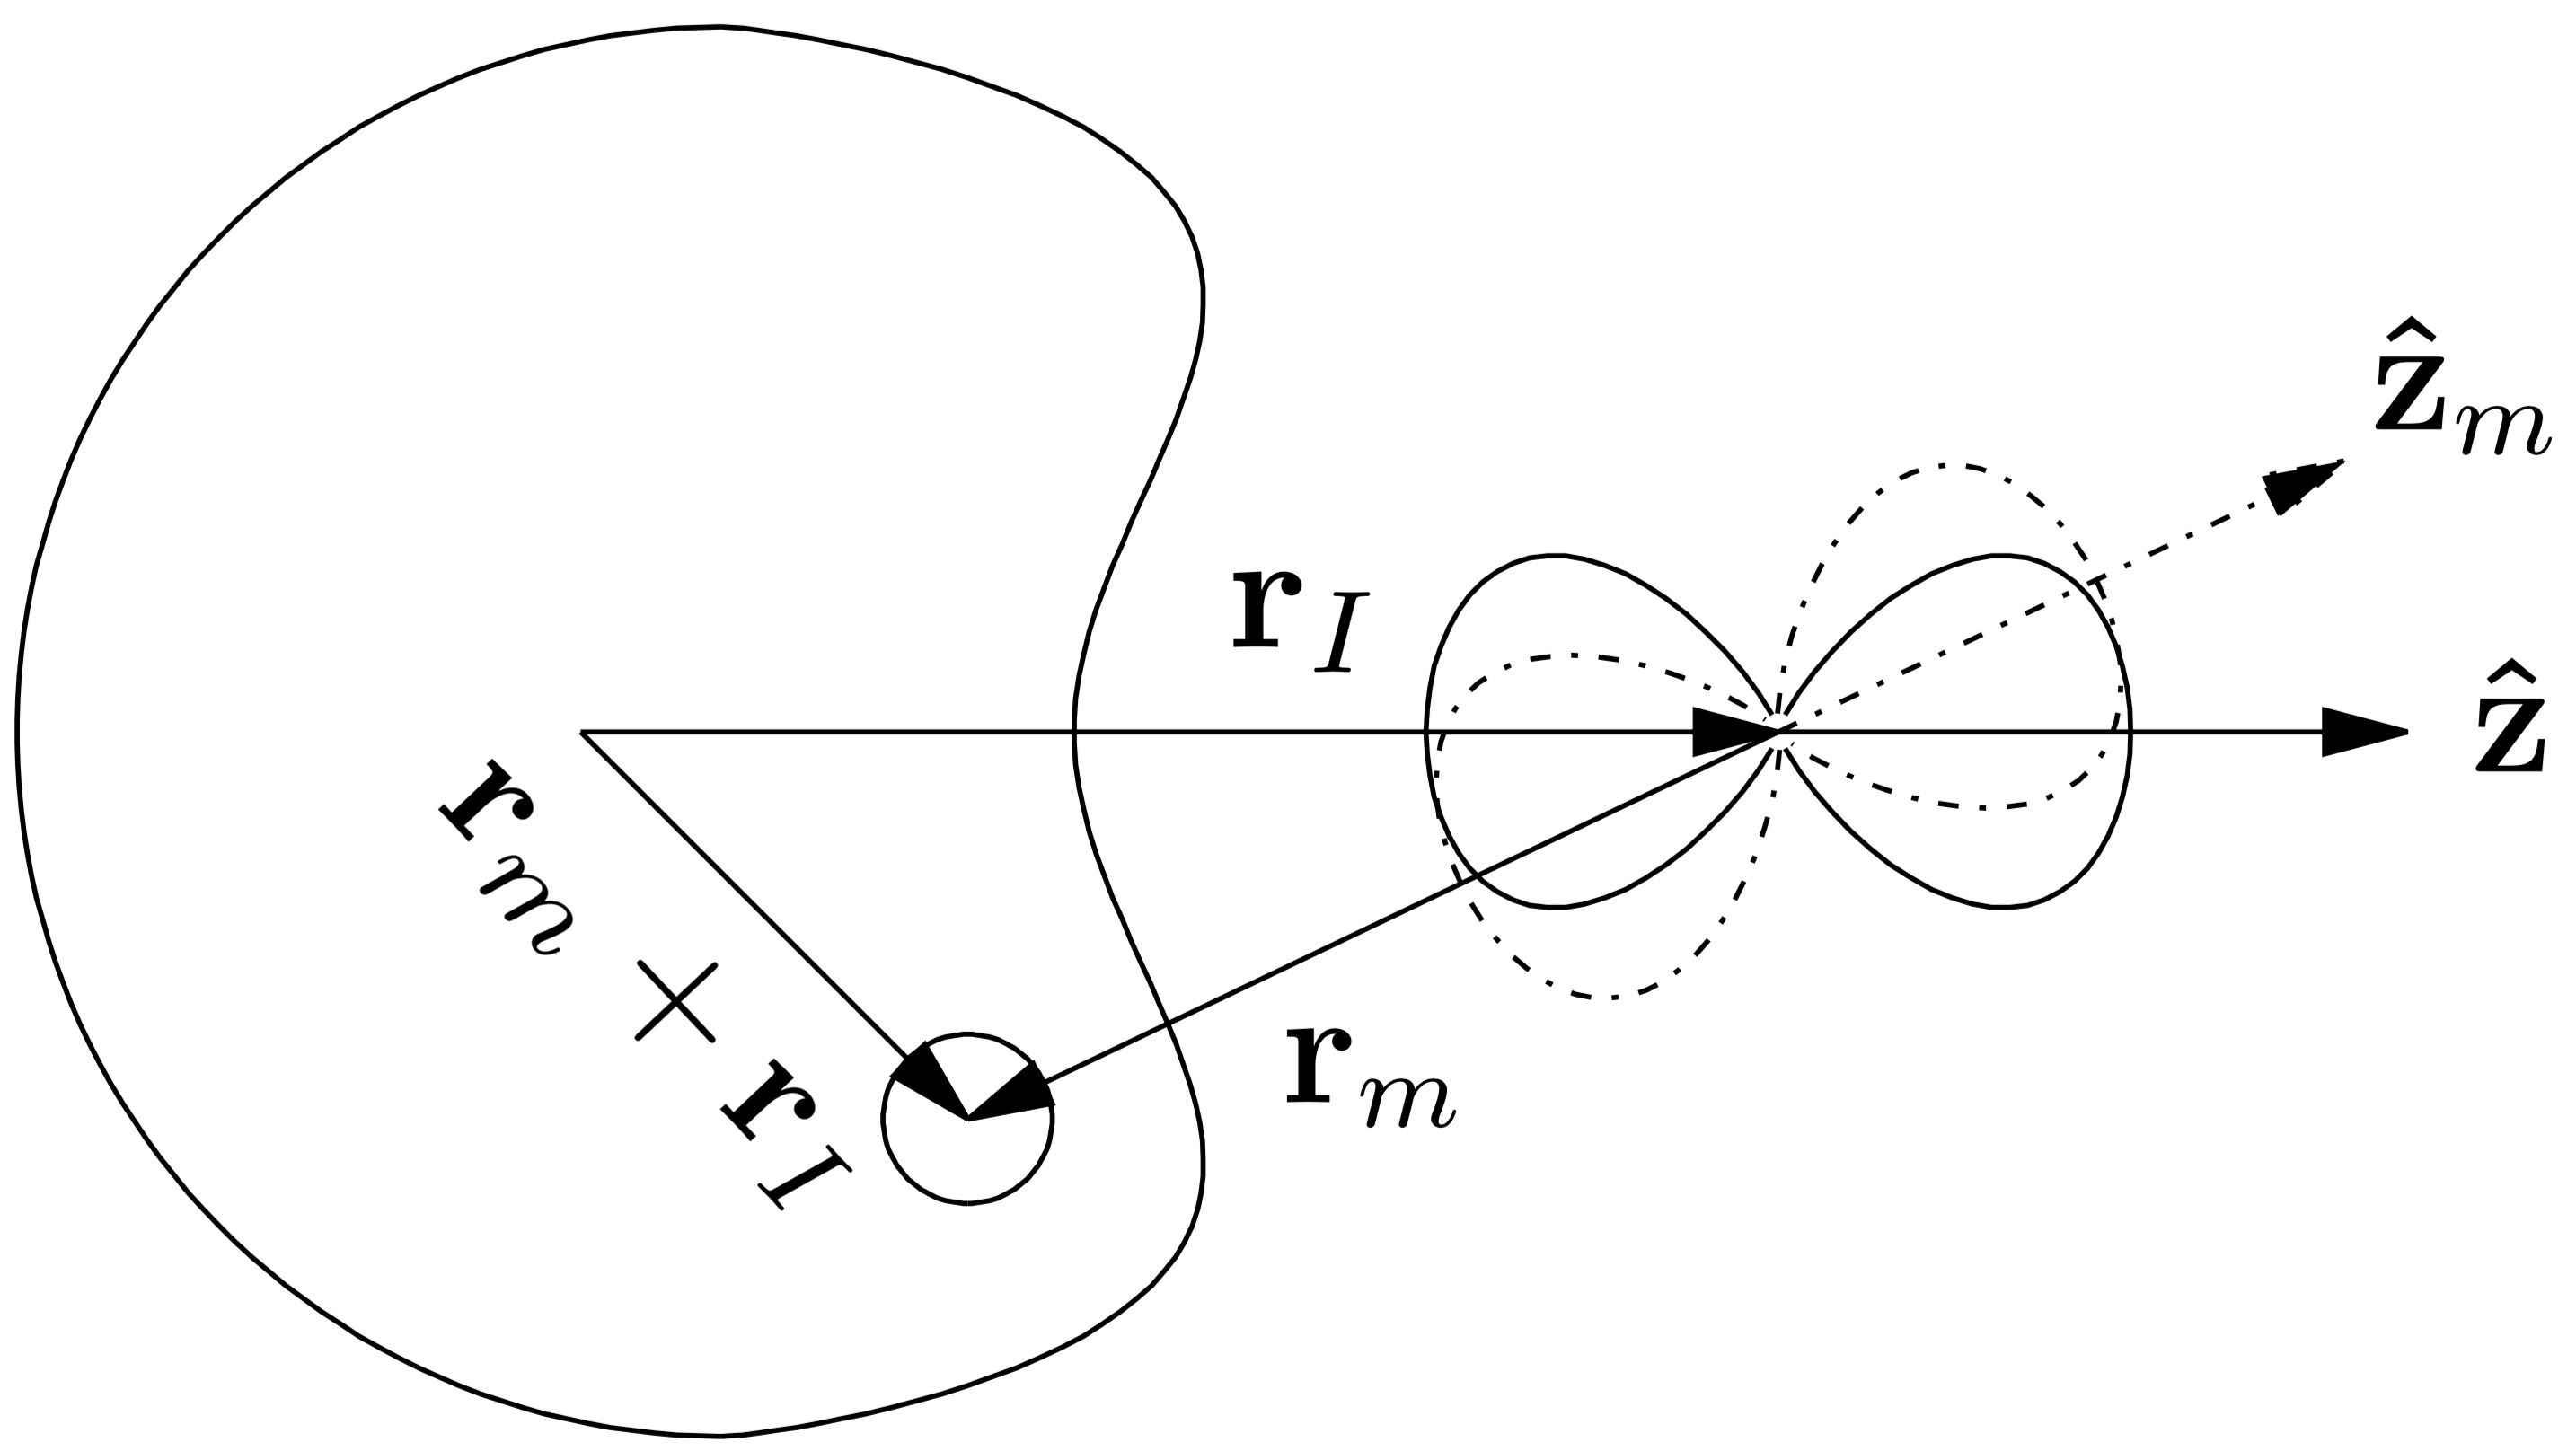
\includegraphics[width=0.75\textwidth]{dim-axes}
				\end{center}
				\caption{The set of axis defined in the DIM description. (Illustration courtesy of M. Martinez\citep{Martinez2017}.)}
				\label{fig:dim-axes}
			\end{figure}			
		
		\subsection{Including spin-orbit coupling}
			For the study of the alkali metal Rb in this work, the spin-orbit (SO) splitting of the energy levels is comparable to the splitting of the orbital angular momentum levels $\Lambda=0$ and $\Lambda=\pm 1$ due to the interaction with the helium. Therefore the spin-orbit interaction needs to be included in the total interaction Hamiltonian.
			
			The total electronic Hamiltonian is given by the sum of the DIM-interaction and the SO-interaction
			\begin{align}
				\mathcal{H} = \mathcal{U}^{DIM}+\mathcal{V}^{SO}.
			\end{align}
			The SO-matrix is approximated by the atomic alkali one, which is approximated by
			\begin{align}
				\mathcal{V}^{SO}=g\vec{L}\vdot\vec{S} = \frac{1}{2}g\qty(\vec{J}^2-\vec{L}^2-\vec{S}^2)
			\end{align}
			The coupling constant $g$ is usually approximated by that of the free atom \cite{Jak97}. We can extend the DIM basis \eq{eq:dim-basis} to include the projection of the electron spin $s=\qty{\uparrow,\downarrow}$ corresponding to the quantum numbers $m_s=\qty{\frac{1}{2},-\frac{1}{2}}$:
			\begin{align}
				\ket{p_i,s}\in\qty\big{\,\ket{p_x,\uparrow}\!,\ket{p_x,\downarrow}\!,\ket{p_y,\uparrow}\!,\ket{p_y,\downarrow}\!,\ket{p_z,\uparrow}\!,\ket{p_z,\downarrow}}.
			\end{align}
			In this basis the matrix $\mathcal{V}^{SO}$ is given by
			\begin{align}
				\mathcal{V}^{SO} = \frac{1}{2}g\mqty*(0&0&-i&0&0&1\\0&0&0&i&-1&0\\i&0&0&0&0&-i\\0&-i&0&0&-i&0\\0&-1&0&i&0&0\\1&0&i&0&0&0)
			\end{align}
			Kramers' theorem states that the two-fold degeneracy of the levels originating from total half-integer spin cannot be broken by electrostatic interactions \cite{Nak01}. Therefore all the electronic eigenstates of $\mathcal{H}$ are doubly degenerate. Diagonalising $\mathcal{H}$ yields three doubly degenerate potential energies between the impurity and surrounding helium.
			
			The dynamic evolution of the electronic excited state of the impurity is described by introducing an additional degree of freedom, a 6-component vector $\ket\lambda$, which describes the coefficients of the electronic state in the $\qty{\ket{p_i,s}}$ basis
			\begin{align}
				\ket{\lambda(t)} = \!\!\!\!\!\sum_{\substack{i=\{x,y,z\}\\s=\{\uparrow,\downarrow\}}}\!\!\!\!\! \lambda_{is}(t) \ket{p_i,s}
			\end{align}
			such that $\norm{\ip{\lambda}}^2=1$. The complete set of variables required to describe the
			system consists of the complex valued effective wave function for helium $\Psi(\mathbf{r}, t)$ with
			$\rho(\mathbf{r}, t) = |\Psi(\mathbf{r}, t)|^2$, the impurity position $\mathbf{r}_I(t)$, and the 6-dimensional complex vector to determine 
			its electronic wave function $|\lambda(t)\rangle$. The total energy of the impurity-$^4$He$_N$ complex after excitation to the $^2$P manifold is

			\begin{align}
				E[\Psi, \vec{r}_I, \lambda] &= \frac{\hbar^2}{2m}\int\!\abs{\grad \Psi}^2\diff{r}
				+ \int\!{\cal E}_c[\rho]\diff{r} \nonumber \\
				&+ \frac{p^2_I}{2 m_I}
				+ \int\!\rho(\vec{r})\,V_\lambda(\vec{r}-\vec{r}_I)\diff{r}
				+ \ev**{\mathcal{V}^{SO}}{\lambda}
			\end{align}
			where $V_\lambda$ is defined as
			\begin{align}
				V_\lambda(\vec{r}) \vcentcolon= \ev{\mathcal{V}^{DIM}}{\lambda} = \sum_{ijss'}\lambda^*_{is}V^{DIM}_{ijss'}(\vec{r})\lambda_{js'} 
			\end{align}
			and the components of the $6\times6$ matrix ${\mathcal V}^{DIM}$ given by
			\begin{equation}
				V^{DIM}_{ijss'}(\vec{r})=V^{DIM}_{ij}\delta_{ss'}=\qty{V_\Pi(r)\delta_{ij}+\qty\big[V_\Sigma(r)-V_\Pi(r)]\frac{r_i\,r_j}{\norm{\vec{r}_m}^2}}\delta_{ss'}
			\end{equation}
			The time evolution of the system is obtained by minimising the following action
			\begin{align}
				A[\Psi,\vec{r}_I,\lambda] = \int\!\bigg\{E[\Psi,\vec{r}_I,\lambda] -&i\hbar\int \!\Psi^*(\vec{r}) \pdv{t}\Psi(\vec{r})\dd{\vec{r}} \nonumber \\
				-&i\hbar\ev**{\pdv{t}}{\lambda} - \frac{1}{2} m_I \dot{\vec{r}}^2_I\bigg\}\dd{t} \label{eq:action}
			\end{align}
			Variation of the action $A$ with respect to $\qty\big{\Psi^*\!,\,\bra\lambda\!,\,\vec{r}_I}$ yields the following three coupled EL-equations
			\begin{align}
				i\hbar\pdv{t}\Psi &= \qty[-\frac{\hbar^2}{2m}\laplacian +\fdv{\mathcal{E}_c}{\rho(\mathbf{r})} + V_\lambda(\vec{r}-\vec{r}_I)]\Psi \nonumber \\
				i\hbar\pdv{t}\ket\lambda  &= \mathcal{H}\ket\lambda \nonumber \\
				m_I\ddot{\vec{r}}_I &= - \grad_{\vec{r}_I}\qty[\int\!\rho(\vec{r})\,V_\lambda(\vec{r}-\vec{r}_I)\dd{\vec{r}}] = -\!\int\!V_\lambda(\vec{r}-\vec{r}_I)\,\grad\rho(\vec{r})\dd{\vec{r}} \label{eq:dyn-el}
			\end{align}
			where the explicit time dependence of the variables is omitted for clarity. The second line of \eq{eq:dyn-el} is a $6\times 6$ matrix equation with the matrix elements of $\mathcal{H}$ given by
			\begin{align}
				H_{ijss'} = U^{DIM}_{ijss'}+V^{SO}_{ijss'} = \int\!\rho(\vec{r})\,V^{DIM}_{ijss'}(\vec{r}-\vec{r}_I)\dd{\vec{r}}+V^{SO}_{ijss'}
			\end{align}
			In the cases that SO-coupling can be neglected the 6-dimensional electronic state vector $\ket{\lambda}$ reduces to the 3-dimensional vector
			\begin{align}
				\ket{\lambda(t)} = \!\sum_{i=\{x,y,z\}} \!\lambda_{i}(t) \ket{p_i}
			\end{align}
			and the $6\times6$ matrix $\mathcal{H}$ reduces to the $3\times 3$ matrix of \eq{eq:u-dim} with elements
			\begin{align}
				H_{ij} = U^{DIM}_{ij} = \int\!\rho(\vec{r})\,V^{DIM}_{ij}(\vec{r}-\vec{r}_I)\dd{\vec{r}}
			\end{align}
			
			For the technical details about how this method is implemented the interested reader is directed to\rf{dft-guide}. For the collection of Fortran code that has been used to obtain the results presented here see\rf{Pi2017}. For the manuel to use the code, with included example calculations see\rf{Coppens2017}.

	\part{Photo-excitation dynamics of alkalis}
		\chapter{Alkali-doped nanodroplets}

	\lettrine[lines=4]{\color{activeColor}I}{n} their 1996 paper\citep{Griffin1996} Griffin and Stringari have argued that almost 100\% Bose-Einstein Condensation could be achieved in the low density surface region of superfluid He at $T=0$, as opposed to only about 10\% in the bulk. It is therefore evident that a minimally perturbing probe capable of investigating the surface of a He cluster is very desirable.

	It was argued from a theoretical perspective\citep{Dalfovo1994} that the alkali atoms reside on the cluster surface. Experimental evidence for this was found\citep{Stienkemeier1995-1,Stienkemeier1995-2,Ancilotto1995-1} later when it was observed that the laser induced fluorescence (LIF) spectrum of sodium was shifted compared to sodium in the gas phase due to the presence of the He cluster. However, not as much as alkali atoms in the bulk of liquid helium.
	
	It comes as no surprise then that alkali atoms are a very natural choice for exactly these type of studies.  For example, with a solvation parameter (see \scn{sec:helium-droplets}) of $\lambda=0.729$\citep{Anc95}, Rb will remain bound to the surface of the droplet. Furthermore, alkalis have a simple, well known, absorption spectrum. Moreover, their simple, one-valence electron structure allows for detailed theoretical modelling. They introduce only weak perturbations (alkali-helium interaction energies are on the order of 1 cm$^{-1}$\citep{Pat91}). Lastly, theoretical calculations\citep{Ancilotto1995-2,Kanorsky1994} and experimental spectra\citep{Tabbert1995,Takahashi1993,Beijersbergen1993} of alkali atoms in bulk liquid helium are available for comparison.

	Surprisingly, the study of alkali atoms seeded in highly quantum matrices is relevant to the optimisation of the use of solid hydrogen as a rocket propellant\citep{Carrick1993}.
	
	Given that alkalis are ideal objects to probe the boundary region of the nanodroplets, the $n\mathrm{p}\,^2\mathrm{P}\!\longleftarrow\!n\mathrm{s}\,^2\mathrm{S}$ transitions of the alkali atoms have attracted much interest from an experimental as well as a theoretical point of view. The spectroscopy of higher excited states has been thoroughly explored\citep{Log11b,Log11a,Lackner2012,Lackner2013,The11,Fec12,Pif10,Lac11,Theisen2011,Lac13}. The obtained spectra can be successfully reproduced by a pseudo-diatomic model\footnote{Also called the ``frozen droplet'' model. It is equivalent to the DIM model, explained in \scn{sec:dim-model}, but where the internal structure of the droplet is neglected, i.e. the whole droplet is considered to be a single huge atom.}, except for the higher excited states, where the model progressively fails due to the limitations imposed by its realm of validity\citep{Sti96,Bunermann2007}. While the the effect of the excited states on the spectra are now fairly well understood, their influence on the following dynamics is largely unexplored.
	
	In this part of the thesis, the results of the real-time dynamics of a single electronically excited rubidium (Rb) atom residing in the surface dimple of a helium nano-droplet are presented. The atom is excited from its ground state 5s$\,^2\Sigma_{1/2}$ to the 5p$\,^2\{\Sigma,\Pi\}$ and 6p$\,^2\{\Sigma,\Pi\}$ manifold (see \scn{sec:dim-model} for an explanation of the used electronic state labels). Usually they desorb upon excitation either as a bare atom or as a complex with one or more helium atoms, called an ``exciplex''.	
	\begin{figure}[t]
		\begin{center}
			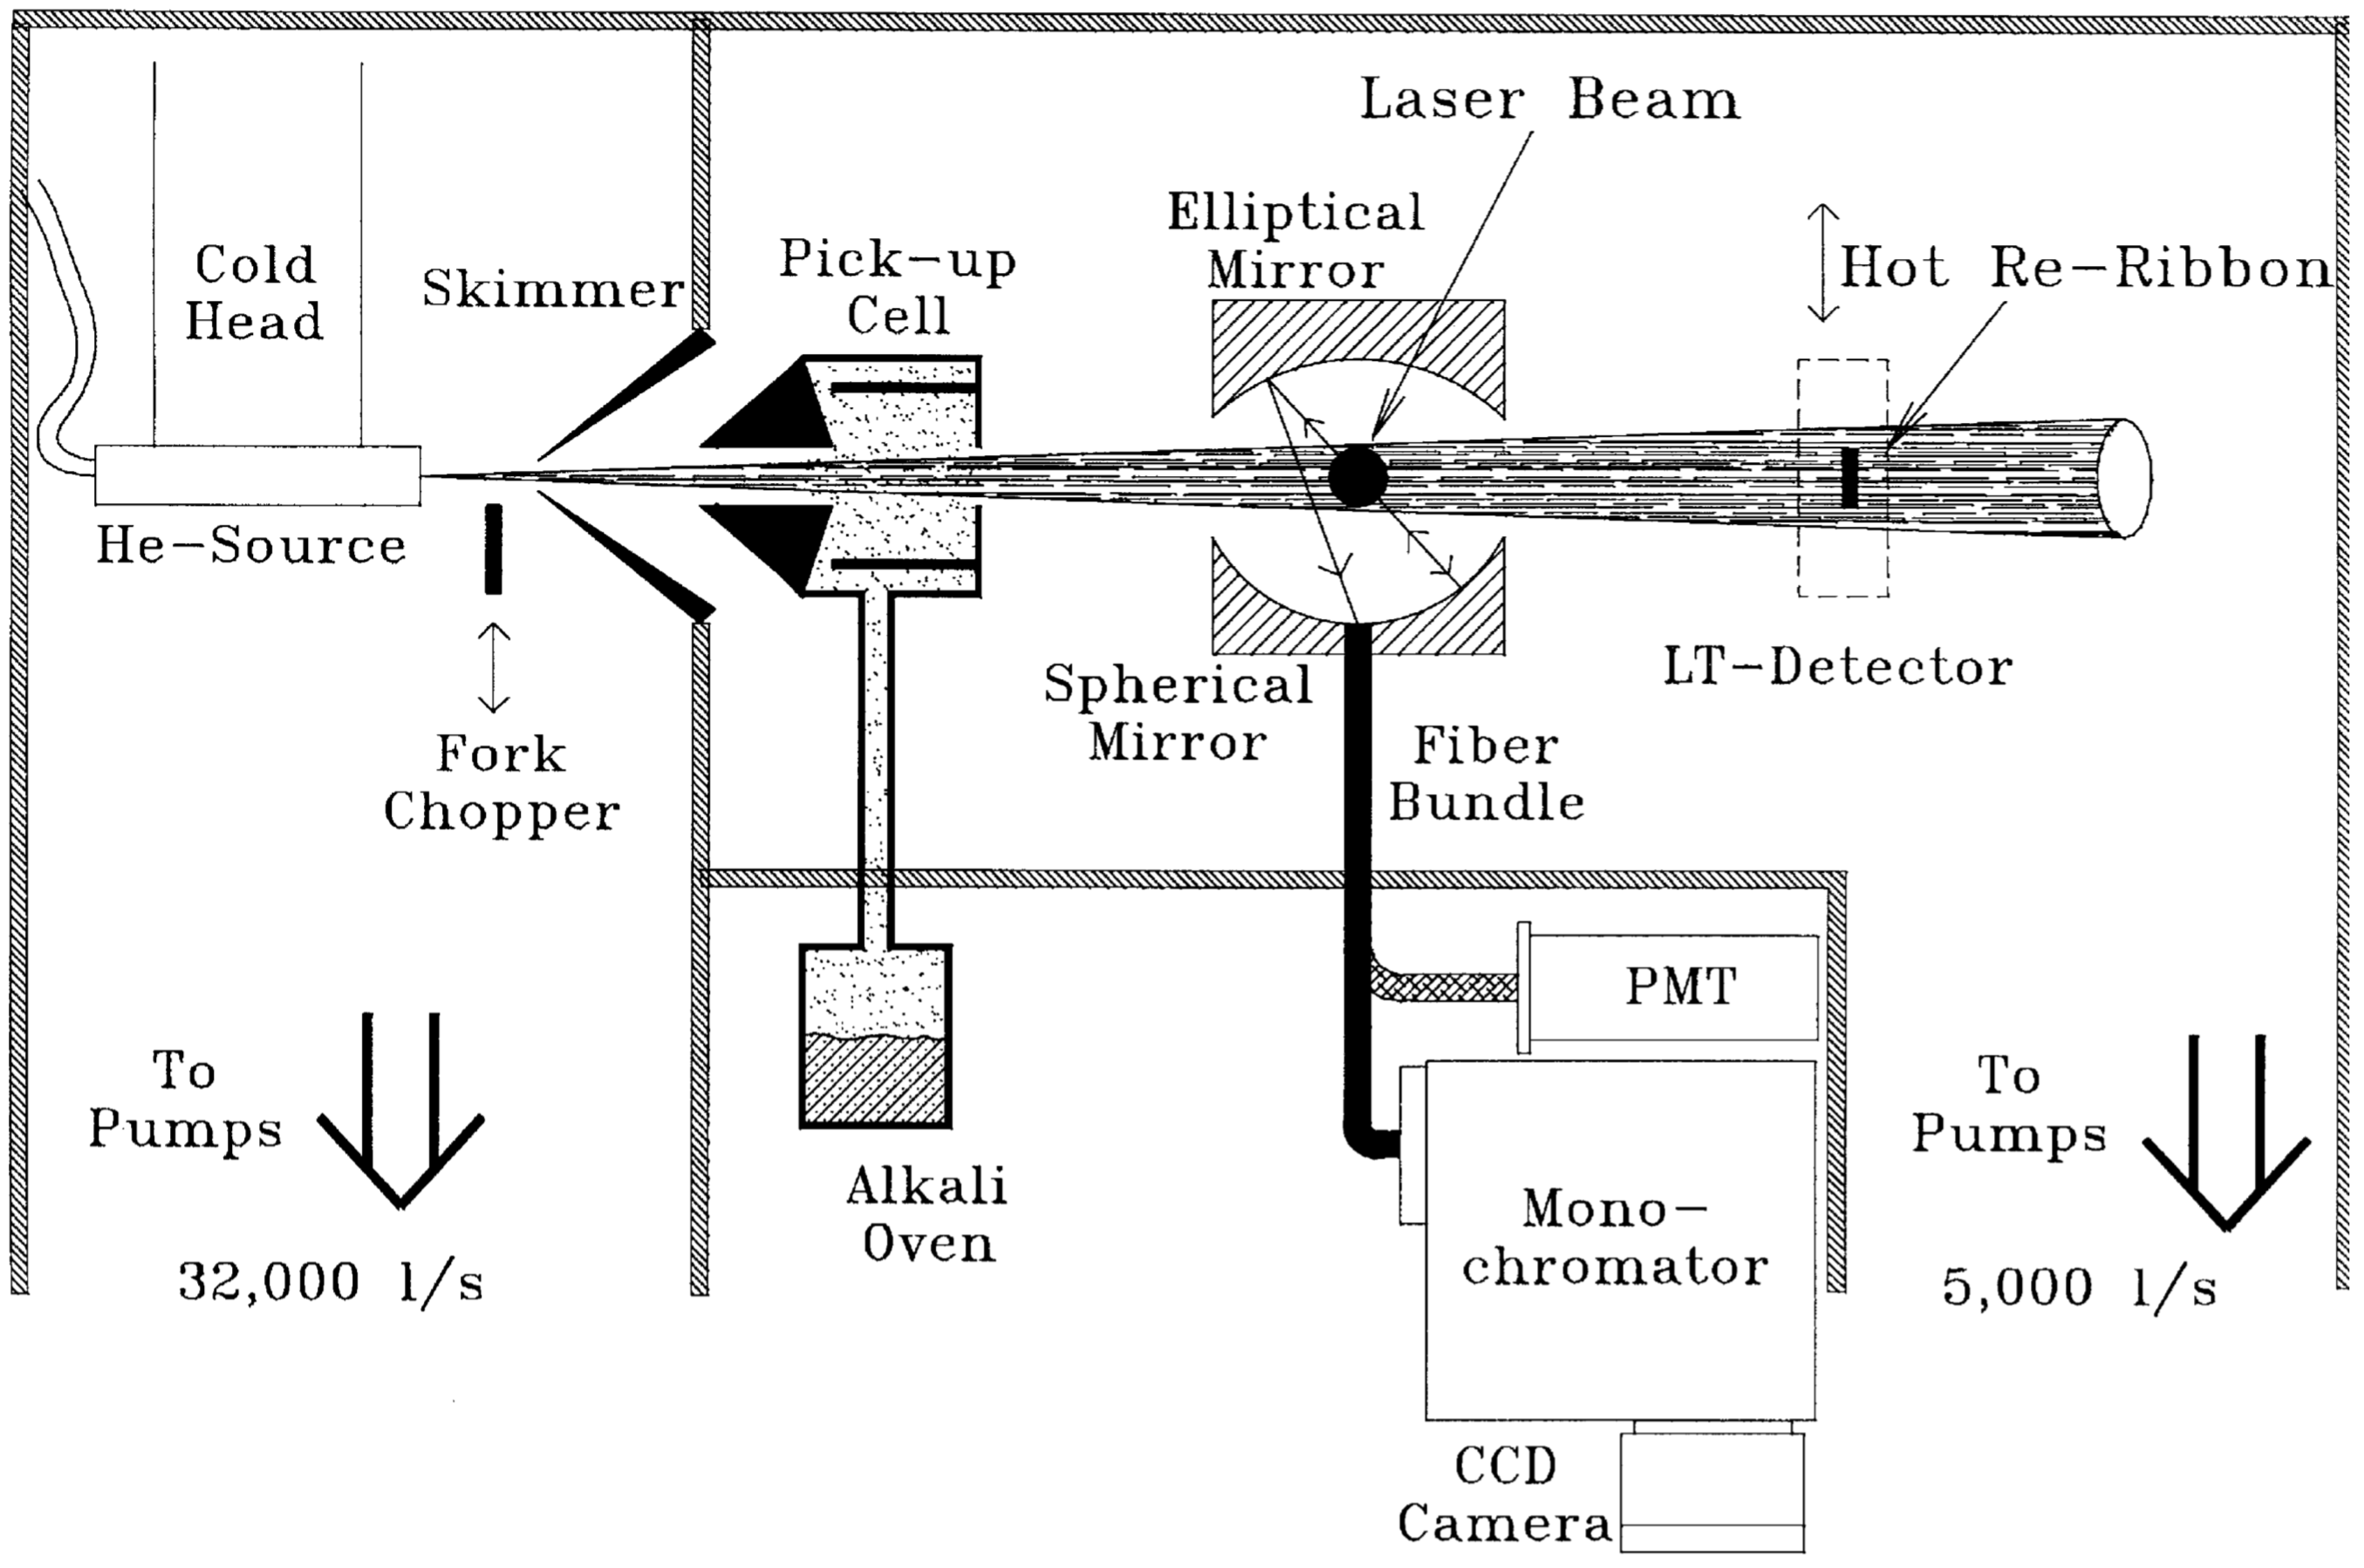
\includegraphics[width=\textwidth]{droplet-beam}
			\caption{Principle of an alkali-doped helium nanodroplet experiment from\rf{Sti96}}
			\label{fig:droplet-beam}
		\end{center}
	\end{figure}
	
	\section*{Experimental setup}
	A beam of large He nanodroplets is produced in a supersonic expansion from a cold nozzle (\fig{fig:droplet-beam}). The weak He-He binding energy of 7.7 cm$^{-1}$ [22] requires high stagnation pressures and low nozzle temperatures ($T$) for large cluster formation. For a set pressure, nozzle aperture and temperature the droplet sizes are log-normal distributed. Doping of the He clusters is realised by sending the beam through a pick-up cell (located a short distance after the skimmer) in which a variable pressure of the alkali is maintained by connecting the pick-up cell with the reservoir through a heated tube. For a chosen average droplet size the average number of dopants picked-up by the droplet is governed by Poissonian statistics and can be controlled with the vapour pressure inside the pickup cell. In their path through the cell the larger clusters pick up alkali atoms without being appreciably deflected. Dissipation of the energy of the captured alkali is likely to occur by evaporation of He atoms from the clusters, the terminal temperature of which rapidly returns to its pre pick-up value ($\sim$0.4 K) [2].

	To probe the picked-up alkali atoms a variety of measurement techniques can be employed, e.g. laser induced fluorescence (LIF) spectroscopy, time-resolved pump-probe spectroscopy, photo-electron spectroscopy and velocity map imaging (VMI). The specific ones used in this work will be introduced generally in the next section.%was used. The intersection point of the laser and cluster beam from which the fluorescence photons are collected is located a few centimetres downstream of the pick-up cell. To detect the fluorescence light originating at the point of intersection, the combination of an elliptical and a spherical mirror is used. These two mirrors focus the emitted photons at the entrance of a fibre bundle. Alternatively, a monochromator coupled to a liquid nitrogen cooled CCD detector is used for dispersed fluorescence measurements.

		\chapter{Results}
	\section{Imaging Excited-State Dynamics}
		\lettrine[lines=3,findent=3pt,nindent=0pt]{T}{he} following article will focus on imaging and characterising the dynamics using femtosecond spectroscopy and time-dependent density functional theory. Specifically on the idea of a fall-back time, which is defined as the time delay $\tau\vcentcolon=t_{ion}-t_{exc}$ between the time instance of the photo-excitation of Rb to the 5p and 6p states, and the time instance of its photo-ionisation, such that the Rb cation is still solvated by the helium droplet.\\
		
		EXPLINAIN SHORT PUMP-PROBE LASER EXPERIMENTS
		
		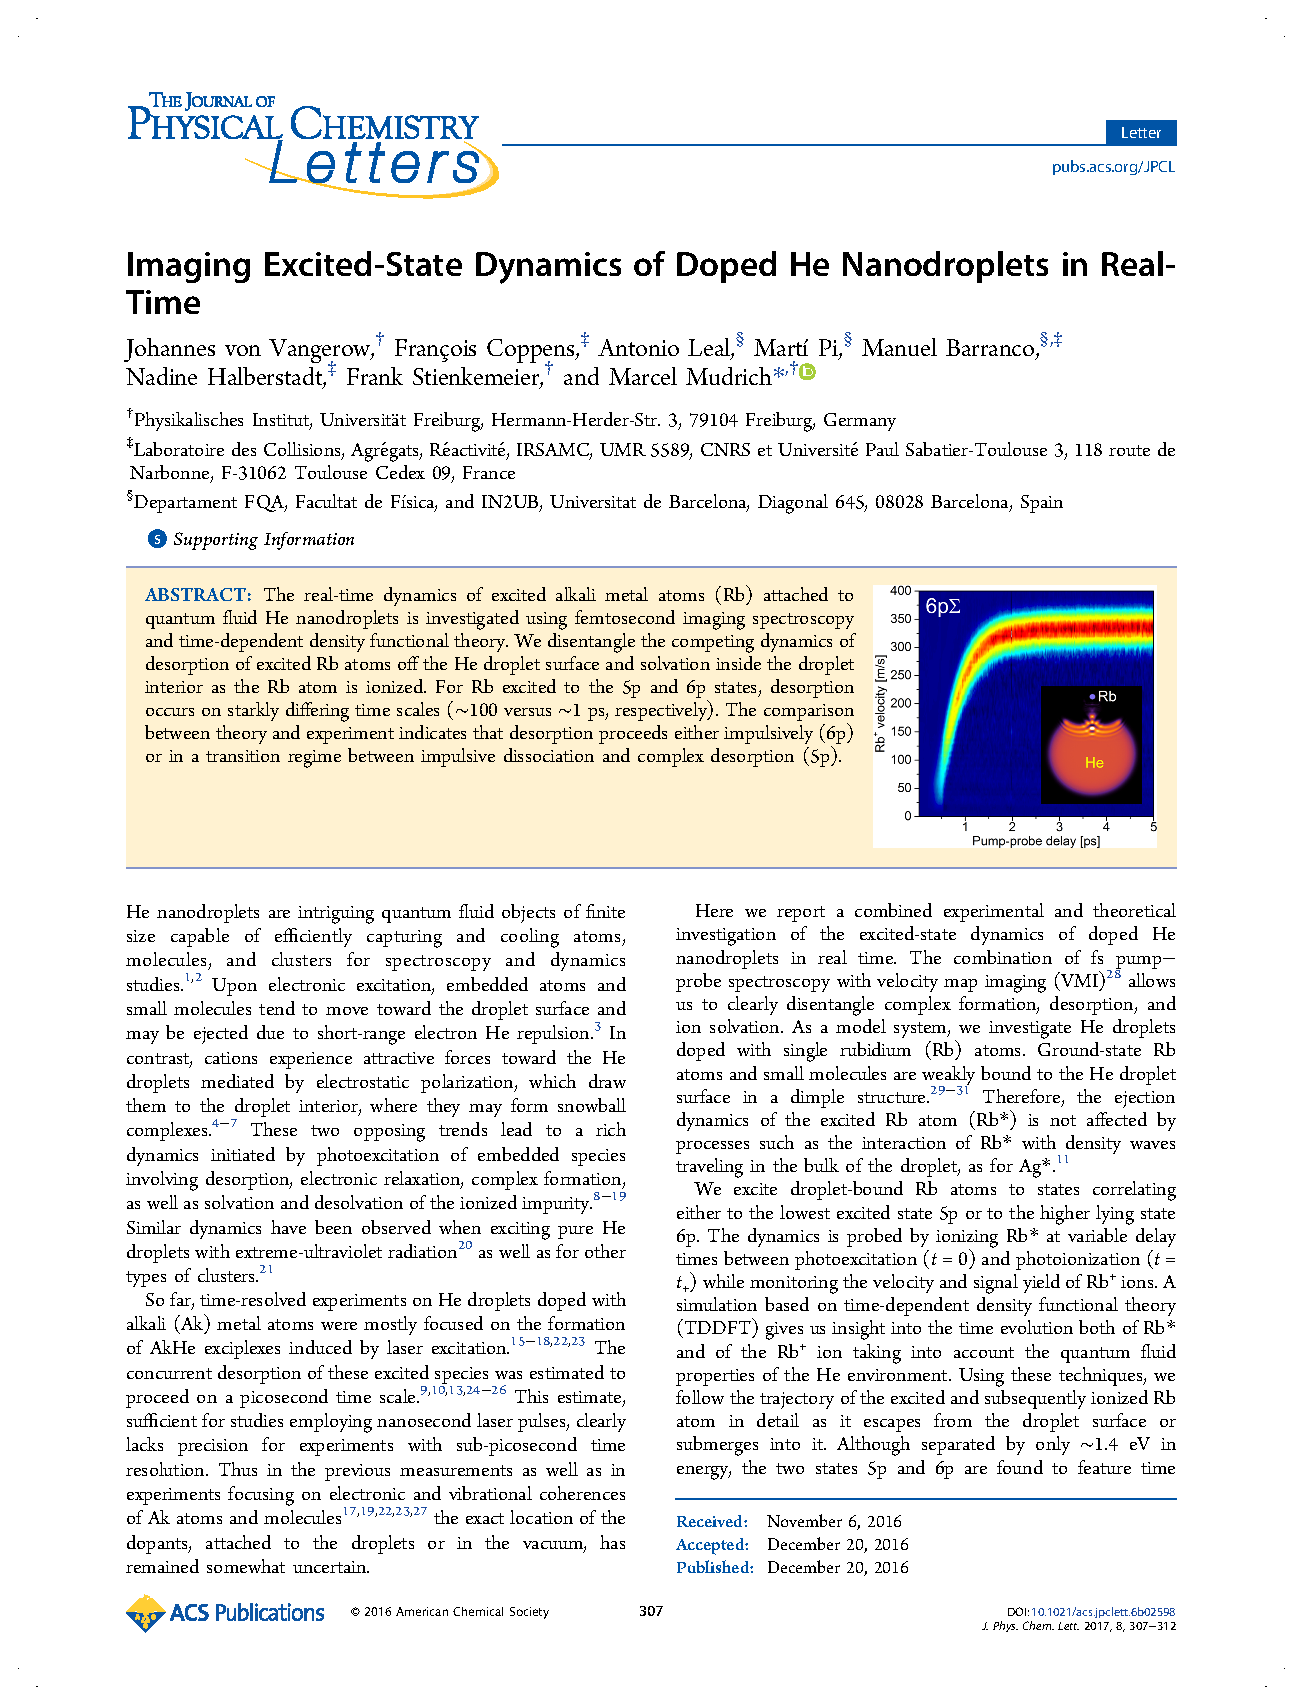
\includepdf[pages=-, scale=0.875, pagecommand={}]{jpcl_vol8_no1_pp307-312.pdf}
		\cleardoublepage

	\section{Desorption dynamics of RbHe exciplexes}
		\lettrine[lines=3,findent=3pt,nindent=0pt]{H}{ow} does a Rb atom, excited to the 5p$\,^2\Pi_{3/2}$ state, detached from a droplets surface---as the experiments show---even tough this is not predicted by TD-DFT calculations? That is the main question that led to this work. Upon photo-excitation of Rb to the 5p$\,^2\Pi_{3/2}$ state, a He atom may be attached to it forming a HeRb exciplex; this cannot happen if Rb is excited to the 5p$\,^2\Pi_{1/2}$ state because it finds a barrier preventing exciplex formation.\\
		
		In the gas phase, a HeRb 5p$\,^2\Pi_{1/2}$ exciplex can be formed if there is enough kinetic energy for Rb* to overcome the potential barrier; alternatively, the collision of the HeRb 5p$\,^2\Pi_{3/2}$ exciplex with another atom or complex might relax the Rb* atom from the 5p$\,^2\Pi_{3/2}$ to the 5p$\,^2\Pi_{1/2}$ state, overcoming the barrier as the potential wells for both states are at similar Rb-He distances. In the condensed (droplet) phase at 0.4 K temperature, none of these mechanisms are active to explain the formation of HeRb 5p$\,^2\Pi_{1/2}$ exciplexes and their potential ejection.\\

		However, a possible mechanism for this is non-radiative de-excitation from the 5p$\,^2\Pi_{3/2}$ to the 5p$\,^2\Pi_{1/2}$ that populates the later state and leaves the Rb* atom with enough kinetic energy so as to be ejected. Notice from the figure that the minimum of the 5p$\,^2\Pi_{3/2}$ potential is 12683 cm1, and that of the 5p$\,^2\Pi_{1/2}$ potential is at 12518 cm1; the value of this potential at the barrier is 12611 cm1. Thus, non-radiative de- excitation of the Rb* atom may add to its original kinetic energy of up to 165 cm1. It is worth noting that it will be ejected in the 5p$\,^2\Pi_{1/2}$ state, and not in the 5p$\,^2\Pi_{3/2}$ it was previously photo-excited.\\
		
		This publication contains a extension of our combined experimental and theoretical investigation presented in the previous section. Here we focus on the formation of free RbHe-exciplex molecules from laser-excited Rb-doped He nanodroplets through the mechanism of electronic spin relaxation. The role of relaxation of internal degrees of freedom of the RbHe exciplex in the desorption process has not been explicitly addressed.
		
		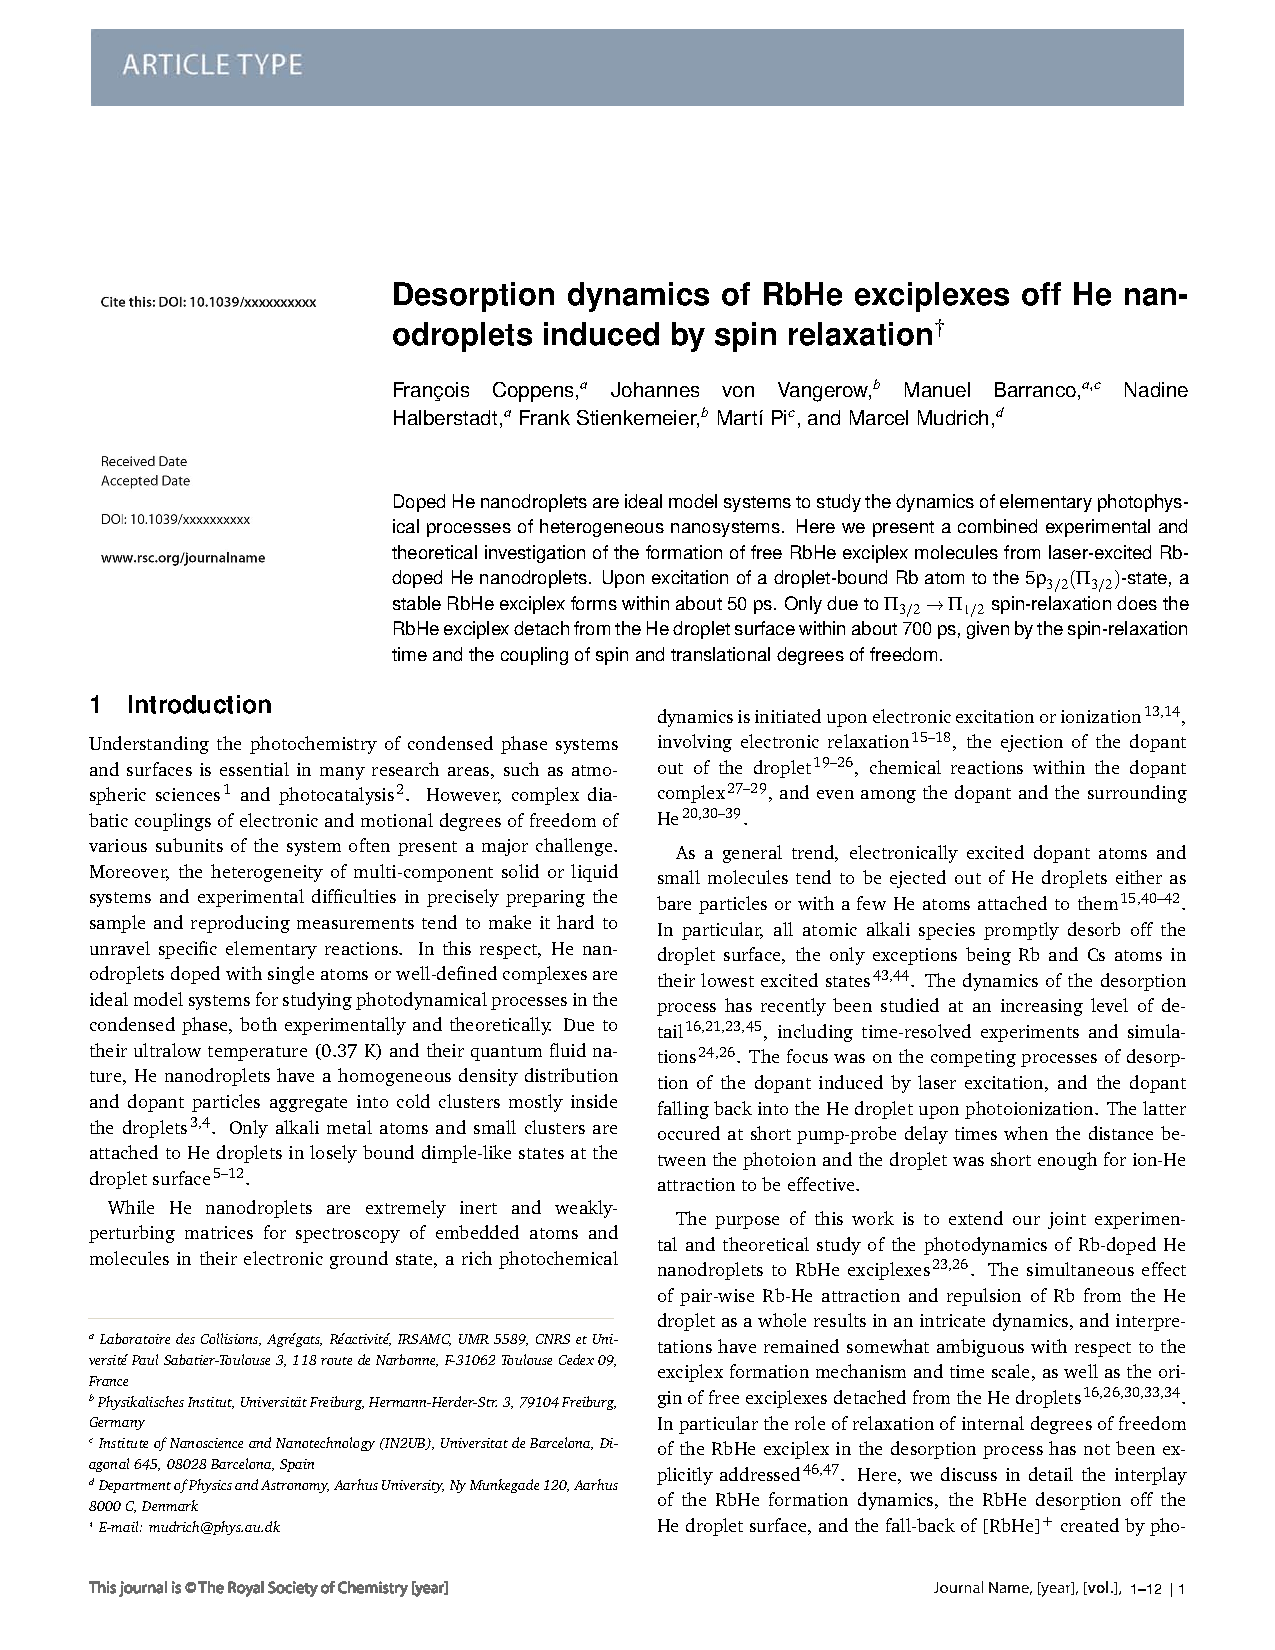
\includepdf[pages={-}, scale=0.8, pagecommand={}]{RbHe-dynamics.pdf}
		\cleardoublepage
		
	\section{Supervised work: potassium-doped\\nanodroplets}
		\lettrine[lines=3,findent=3pt,nindent=0pt]{U}{nder} the supervision of Nadine Halberstadt and me, a master stage -- \emph{M2 Physique Fondamentale} -- titled ``\emph{\textbf{Dynamics of a superfluid helium nanodroplet doped with a single potassium atom}}'' has been performed by Maxime Martinez.\\
	
		The project investigates the static and dynamic behaviour of a single potassium atom excited from the K-$^4$He$_{1000}$ equilibrium configuration to the K*(4p)-$^4$He$_{1000}$ and K*(5s)-$^4$He$_{1000}$ states. The choice of potassium was motivated by a discrepancy in the time-resolved experimental studies\citep{Schulz2001,Reho2000-1,Reho2000-2}. Moreover, the mass of potassium sits between those of the heavier alkalis like rubidium and cesium, and the lighter ones, like lithium and sodium. Therefore, potassium presents an interesting case, being on the borderline between the classical regime for heavy alkalies and a quantum--mechanical regime for the lighter ones. Both treatments of the equilibrium properties and the 5s$\leftarrow$4s excitation are studied. This work is not included in the thesis but can be found in this reference \citep{Martinez2017}.

	\part{Head-on collisions and capture by quantised vortices}
		\chapter{Quantised vortices in droplets}
	One of the most unambiguous signatures of the quantum mechanical nature of a substance---and indeed superfluidity---is the appearance of quantised vortices. In contrast to a normal fluid, which will rotate as a solid body when its container moves at low angular velocity, a superfluid will remain at rest. However, above a certain critical angular velocity the thermodynamically stable state of a superfluid includes one or more quantum vortices. Such a vortex can be characterised by a macroscopic wave function and quantised velocity circulation in units of $\kappa=\frac{h}{m}$, where $h$ is Planck’s constant and $m$ is the mass of the $^4$He atom [2,3]. Recently, the study of vorticity was extended to finite systems such as BECs confined to traps [3,4]. The transfer of energy and angular momentum in finite systems between quantised vortices and surface excitations is of particular interest, as it defines the nucleation dynamics, shape, and stability of the involved vortices [3,4]. In comparison to confined BECs, $^4$He droplets are self-contained and present a case for the strongly interacting superfluid. Moreover, the diameter of a vortex core which is approximately 0.2 nm in superfluid $^4$He [2] is small relative to the droplet size, suggesting a three-dimensionality of the vortices in droplets. Vorticity in $^4$He droplets has therefore attracted considerable interest [5–8].\\
	
	A schematic of the experiment is shown in Fig. \ref{fig:vortex-machine}. Helium droplets are produced by expansion of He, at 20 bar and a temperature $T_0$=5.4--7 K, into vacuum through a nozzle of diameter D 1⁄4 5 "m. The droplets cool rapidly via evaporation and reach a temperature of 0.37 K [20], which is well below the superfluid transition temperature T! 1⁄4 2:17 K [2,3]. Further downstream, the droplets capture 103–106 Ag atoms in an oven [21]. The droplets are then collided against a thin carbon film substrate at room temperature [21]. Upon impact, the droplets evaporate, leaving on the surface the Ag traces, which are subsequently imaged via a transmission electron microscope (TEM).
	\begin{figure}[t]
		\begin{center}
			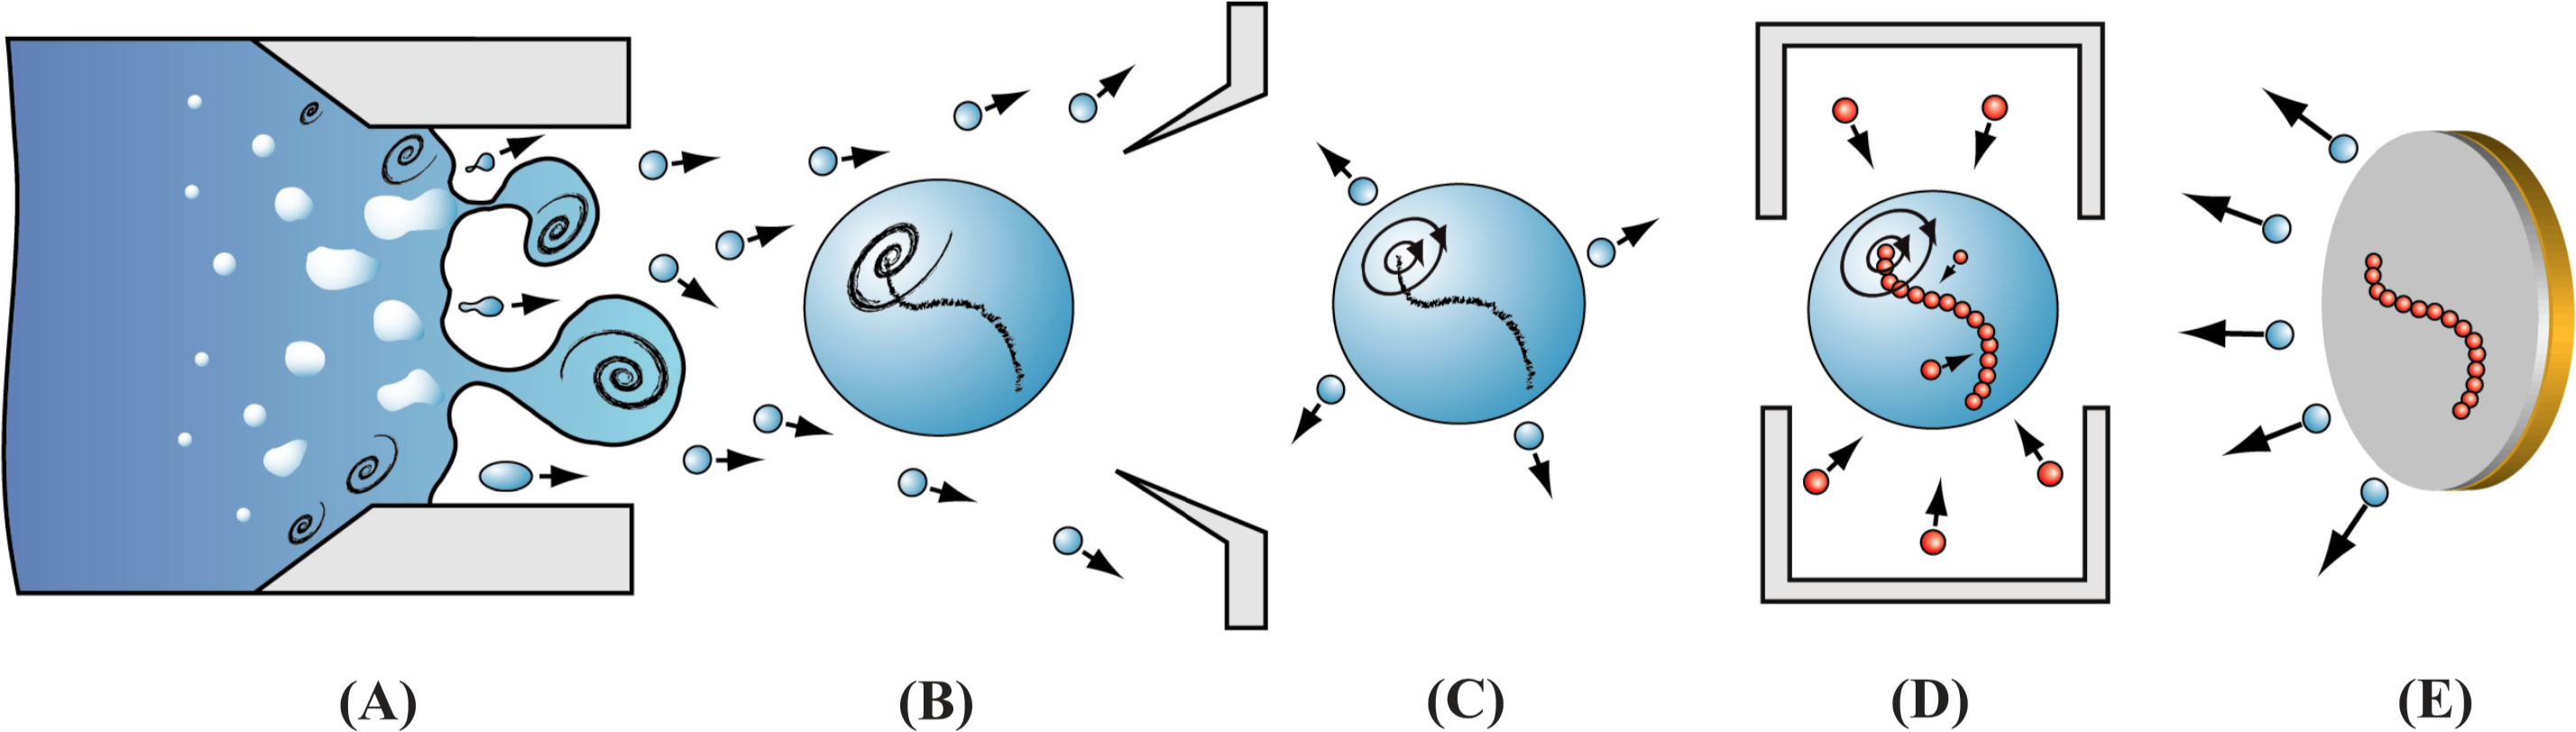
\includegraphics[width=\textwidth]{vortex-machine}
			\caption{Schematic of the experiment. (a) He fluid expands in vacuum and (b) breaks up into rotating droplets. (c) A quantum vortex is formed as a consequence of fast evaporative cooling of the droplet to below $T_\lambda$. (d) The droplet is doped with Ag atoms, which are attracted to the vortex core. (e) The droplet then collides with the carbon surface leaving behind the Ag trace, whereas the He evaporates.}
			\label{fig:vortex-machine}
		\end{center}
	\end{figure}	
	
	Recently, Gomez, Loginov and Vilesov performed experiments[PRL 108, 155302 (2012)] where vortices inside superfluid $^4$He droplets, produced by the expansion of liquid helium, were traced by introducing Ag atoms which clustered along the vortex lines, into the droplets. The Ag clusters were subsequently surface-deposited and imaged via electron microscopy. The prevalence of elongated track-shaped deposits (see Figure \ref{fig:silver-filament}) shows that vortices are present in droplets larger than about $300\unit{nm}$ and that their lifetime exceeds a few milliseconds. Two years later Gomez reported[Science 345, 906 (2014)] on the formation of quantum vortex lattices inside droplets. He used single-shot femtosecond x-ray coherent diffractive imaging to investigate the rotation of single, isolated superfluid helium-4 droplets containing $\sim\!10^8$ to $10^{11}$ atoms. The formation of quantum vortex lattices inside the droplets was confirmed by observing the characteristic Bragg patterns from xenon clusters trapped in the vortex cores (see Figure \ref{fig:vortex-array}).

	\begin{figure}[t]
		\begin{center}
			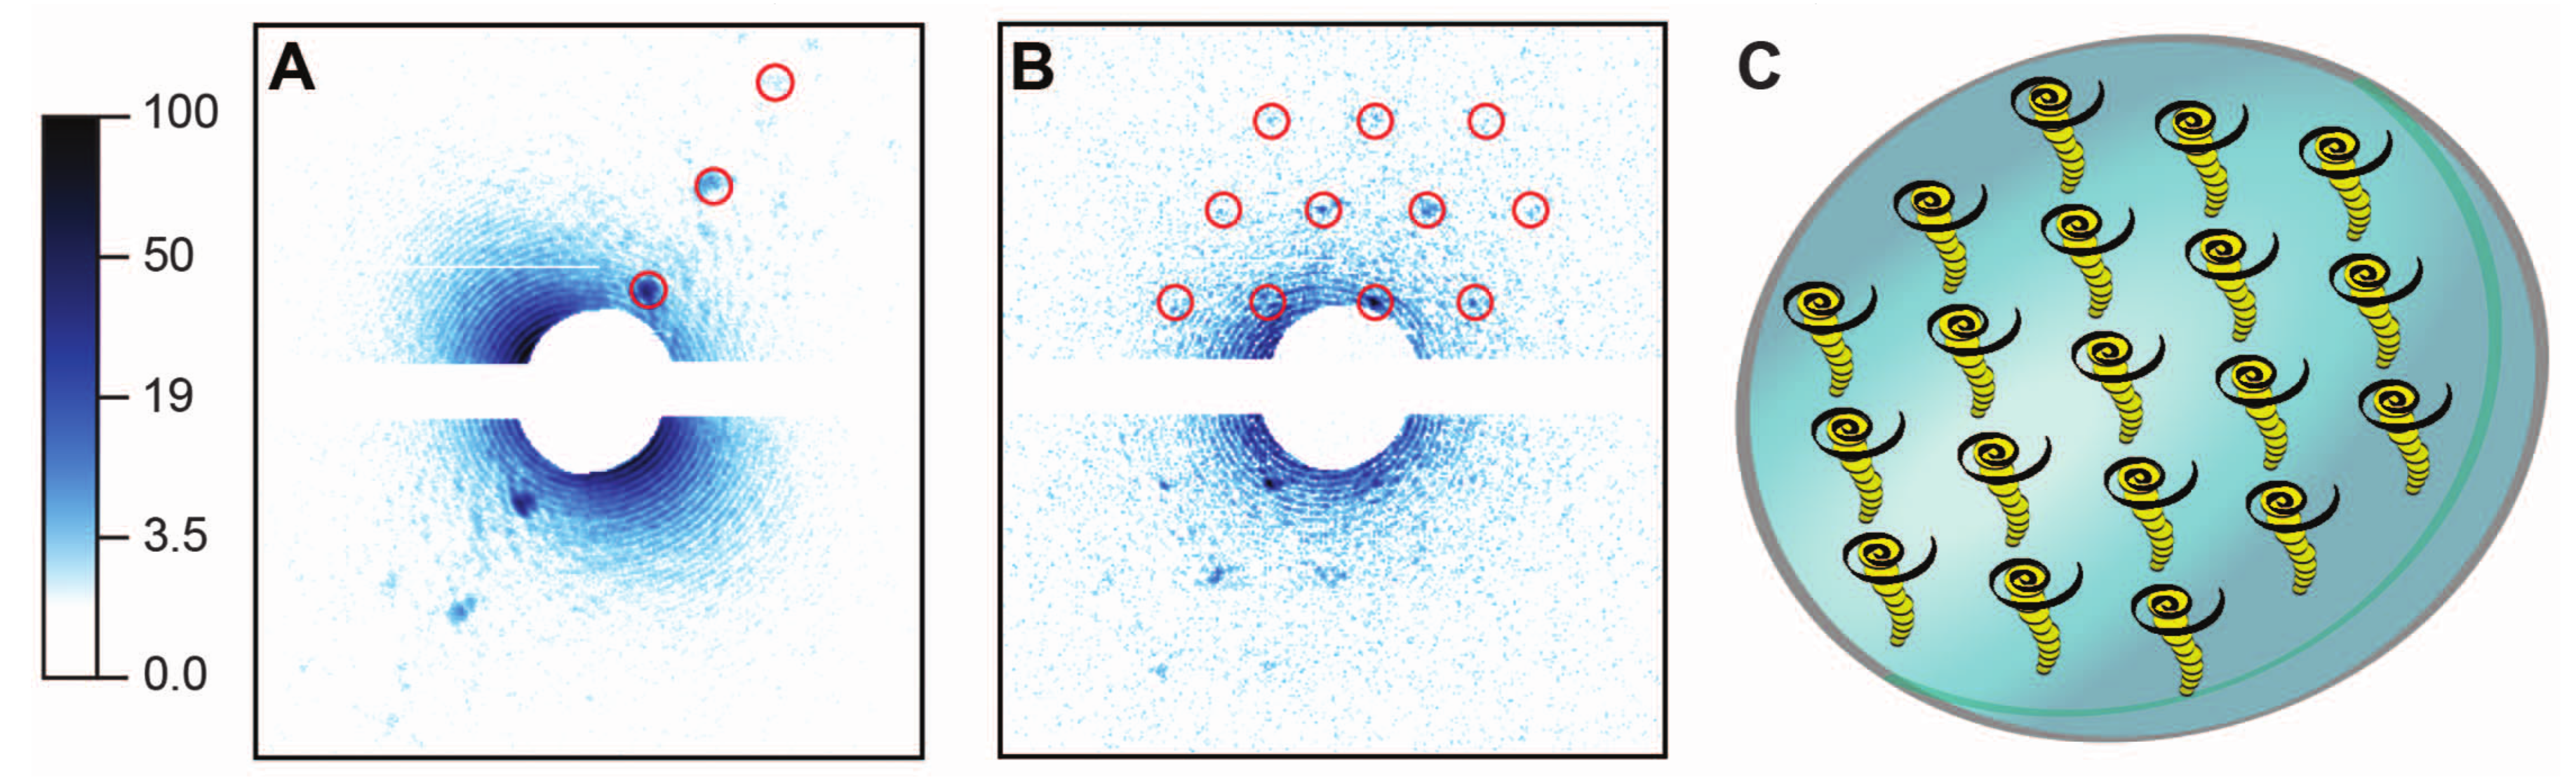
\includegraphics[width=\textwidth]{vortex-array}
			\caption{He droplets doped with Xe atoms. (A and B) X-ray diffraction images of doped droplets, displayed in a logarithmic intensity scale. (C) Droplet and embedded Xe clusters. Images in (A) and (B) correspond to tilted and parallel alignments of the vortex axes with respect to the incident x-ray beam, respectively.}
			\label{fig:vortex-array}
		\end{center}
	\end{figure}
	
%	\section{Head-on collisions}
%		\lettrine[lines=3,findent=3pt,nindent=0pt]{I}{t} is well known that helium drops readily capture foreign atoms and molecules[1], and this ability has had a considerable influence on the chemistry and physics of these systems[2]. Among the studies carried out in the past on atom-drop collisions, let us mention those aiming at experimentally determining the density profiles of large $^4$He and $^3$He droplets from the scattering of Ar and Kr atoms off helium droplets, which have been analysed within density functional theory (DFT)[3,4]; the microscopic simulation of the scattering of 3He and 4He atoms from inhomogeneous liquid helium systems[5,6]; and an earlier theoretical work on the scattering of 4He atoms from 4He droplets within a liquid drop plus optical model approach[7].\\
%
%		Very recently, time-dependent density functional theory (TDDFT) has been used to address the capture of Cs or Ne atoms by $^4$He nanodroplets[8,9]. The Cs capture was treated fully three dimensionally with the Cs atom described as a classical particle, whereas for the Ne capture study the Ne atom was described quantum mechanically, but the description was strictly one dimension.\\
%
%		Motivated by recent experiments that use Xe atoms to visualise vortex arrays in very large helium droplets[10,11], we present here a first step toward the description of the capture of Xe atoms by helium droplets, namely head-on collisions of Xe atoms against a $^4$He$_{1000}$ droplet. A discussion on the dynamic capture of Xe atoms by droplets hosting vortex lines and vortex arrays will be provided by a forthcoming study combining DFT simulation of vortex arrays as in Refs.[12,13] for helium nanocylinders and nanodroplets and collision with Xe atoms as in this work. Whenever possible, the results for Xe, a heliophilic atom, are contrasted with results for Cs, a heliophobic atom with similar mass.
%
%	\section{Capture by quantised vortices}
%		\lettrine[lines=3,findent=3pt,nindent=0pt]{I}{t} is well established that helium droplets can readily capture in their interior almost any atom or molecule interacting with them, as first shown for the case of Ne atoms[1], with the notable exception of alkali[2] and some alkaline-earth[3] atoms. This property, together with the extremely low temperature (T) achieved in helium droplets -- of the order of 0.4 K -- makes them the perfect ultracold and inert environment for hosting and studying isolated atoms and molecules, which is at the basis of current applications of helium droplets for spectroscopic studies of atoms and molecules. Besides, the superfluid nature of helium facilitates binary encounters of atoms/molecules in the bulk of the droplet while absorbing the energy released upon recombination, making possible chemical reactions which would not otherwise occur in the gas phase. These unique properties of helium droplets have had a huge impact on their study[4-8].\\
%
%		The pickup of Ar, Kr and Xe atoms in the gas phase by $^4$He$_N$ droplets with $N>10^3$ atoms produced by nozzle beam expansions was described about twenty years ago by Toennies and coworkers[9]. In these experiments, the droplets in the helium beam were deflected by impacting with a secondary beam made of rare gas atoms.\\
%
%		Recently, a technique has been introduced to determine the size of large He droplets ($N>10^5$). It is based on the attenuation of a continuous droplet beam through collisions with Ar atoms at room temperature[10]. The pickup chamber of the droplet beam apparatus is filled with argon gas and the helium droplets experience multiple, isotropic collisions with the Ar atoms on their way towards the detection chamber. Large helium droplets could also be doped in this way. This method, using Xe atoms, has been instrumental for detecting and imaging quantised vortex arrays in helium droplets[11,12]. Xe atoms were used in these experiments because of their large sensitivity to the X-ray coherent diffractive imaging employed to detect them within the helium droplets. Experiments with large superfluid helium droplets are reviewed in a recent publication[14].\\
%
%		The impurity-droplet interaction in the presence of vortices is also relevant as the first stage of a more complex process leading to the formation of nanowires, see e.g. ref. 15-18. Long filaments made of micrometer-sized solid hydrogen particles trapped on quantised vortex cores were used to directly image the vortex reconnection between quantised vortices in superfluid helium[19].\\
%
%		The impact and capture of impurities interacting with pure helium droplets have been addressed recently within time-dependent density functional theory (TDDFT). Real-time simulations have been carried out for heliophobic[20] (Cs) and heliophilic[21] (Ne) atoms. In addition to the TDDFT equation for $^4$He, heavy impurities are treated as classical particles using Newton's equation of motion, whereas a time-dependent Schr\"{o}dinger equation has been used in the case of light impurities within the mean field model[21,22]. A comparison between the results for head-on collisions of Cs and Xe atoms -- heliophobic and heliophilic atoms of similar mass -- has been presented in ref. 23.\\
%
%		In this work, we present the results obtained within TDDFT for the collision and capture of Xe and Ar atoms by a $^4$He$_{1000}$ droplet at different kinetic energies and impact parameters. Special attention is paid to the time-dependent interaction of Xe and Ar atoms with helium nanodroplets hosting vortex lines, and to the effect of multi-doped vortex arrays in large helium droplets.\\
%
%		Due to the heavy computational cost of the TDDFT simulations presented here, we address only a few facets of the capture process that we consider of experimental relevance rather than carrying out a systematic study of the process. In particular:
%		\begin{itemize}
%			\item We study the capture of Xe atoms by a $^4$He nanodroplet, both for head-on collisions and for different impact parameters, with velocities ranging from thermal values up to several hundred m/s. The results of peripheral collisions with different values of the impact parameter are used to estimate the cross section for the Xe capture.
%			\item We study how a Xe atom dynamically interacts with a droplet hosting a vortex line, under different initial conditions resulting in different velocity regimes of the impurity as it collides with the vortex core: 
%			\begin{enumerate}
%				\item[i)] a Xe atom initially at rest on the droplet surface and sinking under the effect of solvation forces
%				\item[ii)] a head-on collision of a moving Xe or Ar atom against the $^4$He nanodroplet.	
%			\end{enumerate}
%			\item We study the stationary state of a large $^4$He$_{15000}$ droplet hosting a ring of six vortex lines, doped with Ar atoms completely filling all six vortex cores. This is the simplest system that mimics those experimentally described in ref. 11, where doped vortex arrays embedded in rotating $^4$He microdroplets have been imaged.
%		\end{itemize}
%
%		Multimedia materials accompany this paper, showing the real-time dynamics of several impact/capture processes described here. These materials are presented in the ESI document. They constitute an important part of this work, since often it is only by viewing how a complex microscopic process unfolds in real-time that one can catch important physical details which would otherwise escape in a written account.
		\chapter{Head-on collisions of Xe and Cs}	
	\section{Introduction}
		It is well known that helium drops readily capture foreign atoms and molecules \citep{Sch90}, and this ability has had a considerable influence on the chemistry and physics of these systems \citep{Toe04}. Among the studies carried out in the past on atom-drop collisions, let us mention those aiming at experimentally determining the density profiles of large $^4$He and $^3$He droplets from the scattering of Ar and Kr atoms off  helium droplets, which have been analyzed within density functional theory  (DFT) \citep{Har98,Har01}; the microscopic simulation of the scattering of $^3$He and $^4$He atoms from inhomogeneous liquid helium systems \citep{Kro07,Kro08}, and an earlier theoretical work on the scattering of $^4$He atoms from $^4$He droplets within a liquid drop plus optical model approach\citep{Eic88}.

		Very recently, time-dependent density functional theory (TDDFT) has been used to address the capture of Cs or Ne atoms by $^4$He nanodroplets \citep{Lea14a,Vil16b}. The Cs capture was treated fully three dimensionally with the Cs atom described as a classical particle, whereas for the Ne capture study the Ne atom was described quantum-mechanically but the description was strictly one-dimensional.
			
		Motivated by recent experiments that use Xe atoms to visualise vortex arrays in very large helium droplets \citep{Gom14,Jon16}, we present here a first step towards the description of the capture  of Xe atoms by helium droplets, namely head-on collisions of Xe atoms against a $^4$He$_{1000}$ droplet. A discussion on the dynamic capture of Xe atoms by droplets hosting vortex lines and vortex arrays will be provided by a forthcoming study combining DFT simulation of vortex arrays as in Refs.\citen{Anc14,Anc15} for helium nanocylinders and nanodroplets  and collision with Xe atoms as in this work. Whenever possible, the results for Xe, a heliophilic atom,  are contrasted with results for Cs, a heliophobic atom with similar mass. We use TD-DFT as described in Section \ref{sec:td-dft}. 

		\begin{figure}[!] 
			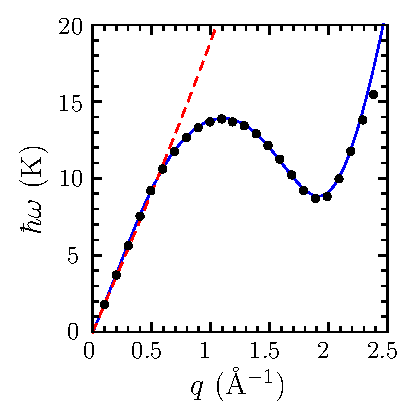
\includegraphics[width=1.0\linewidth,clip=true]{fig1}
			\caption{ \label{fig1-headon} Energy of the Xe@$^4$He$_{1000}$ complex as a function of the distance between  the Xe atom and the  COM of the droplet. Several two-dimensional helium densities and density profiles are shown for distances between 0 and 40 \AA{} in 5  \AA{} steps. Connected (dots) and disconnected (triangles) helium configurations are shown \emph{(see text)}. Top left inset: Snapshot of the helium density at the first turning point  during the dynamic evolution of a Xe atom (green dot) at $v_0 = 600$ m/s attained  78 ps after it has started. (Color figure online.)}
		\end{figure}

	\section{Results}

		\begin{figure}[!]
			\centerline{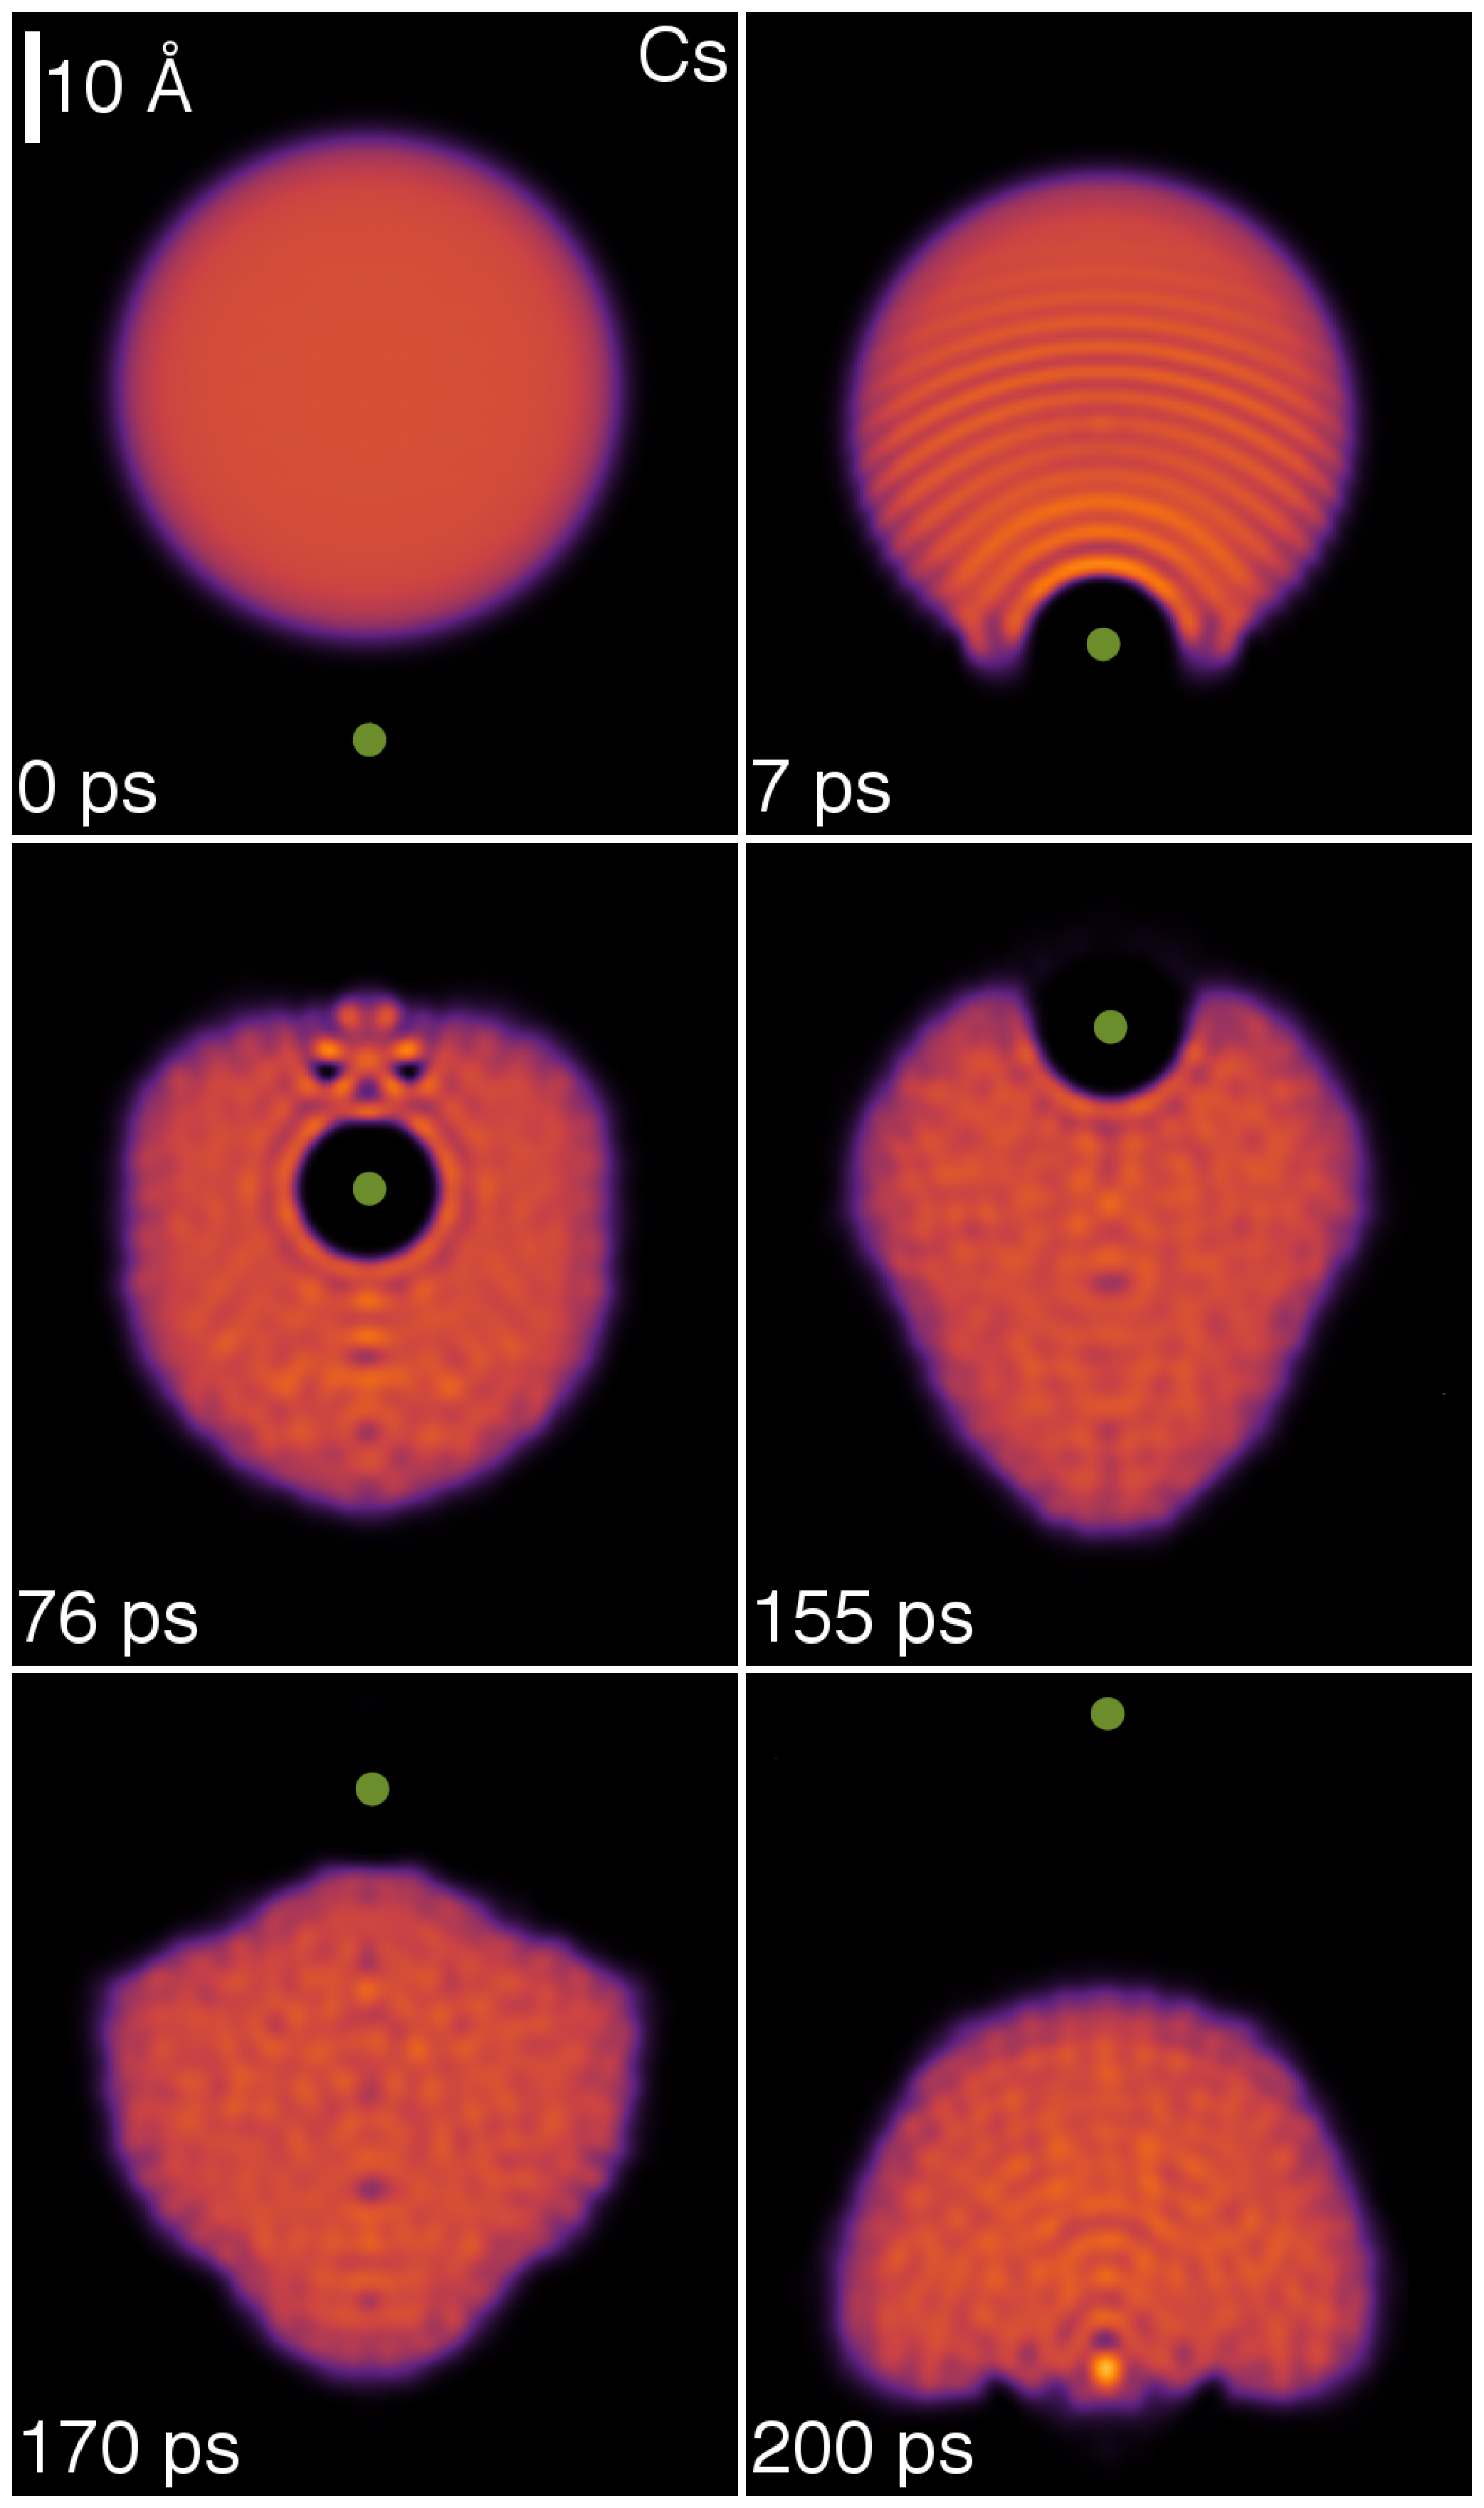
\includegraphics[width=0.50\linewidth,clip]{fig2-Cs} 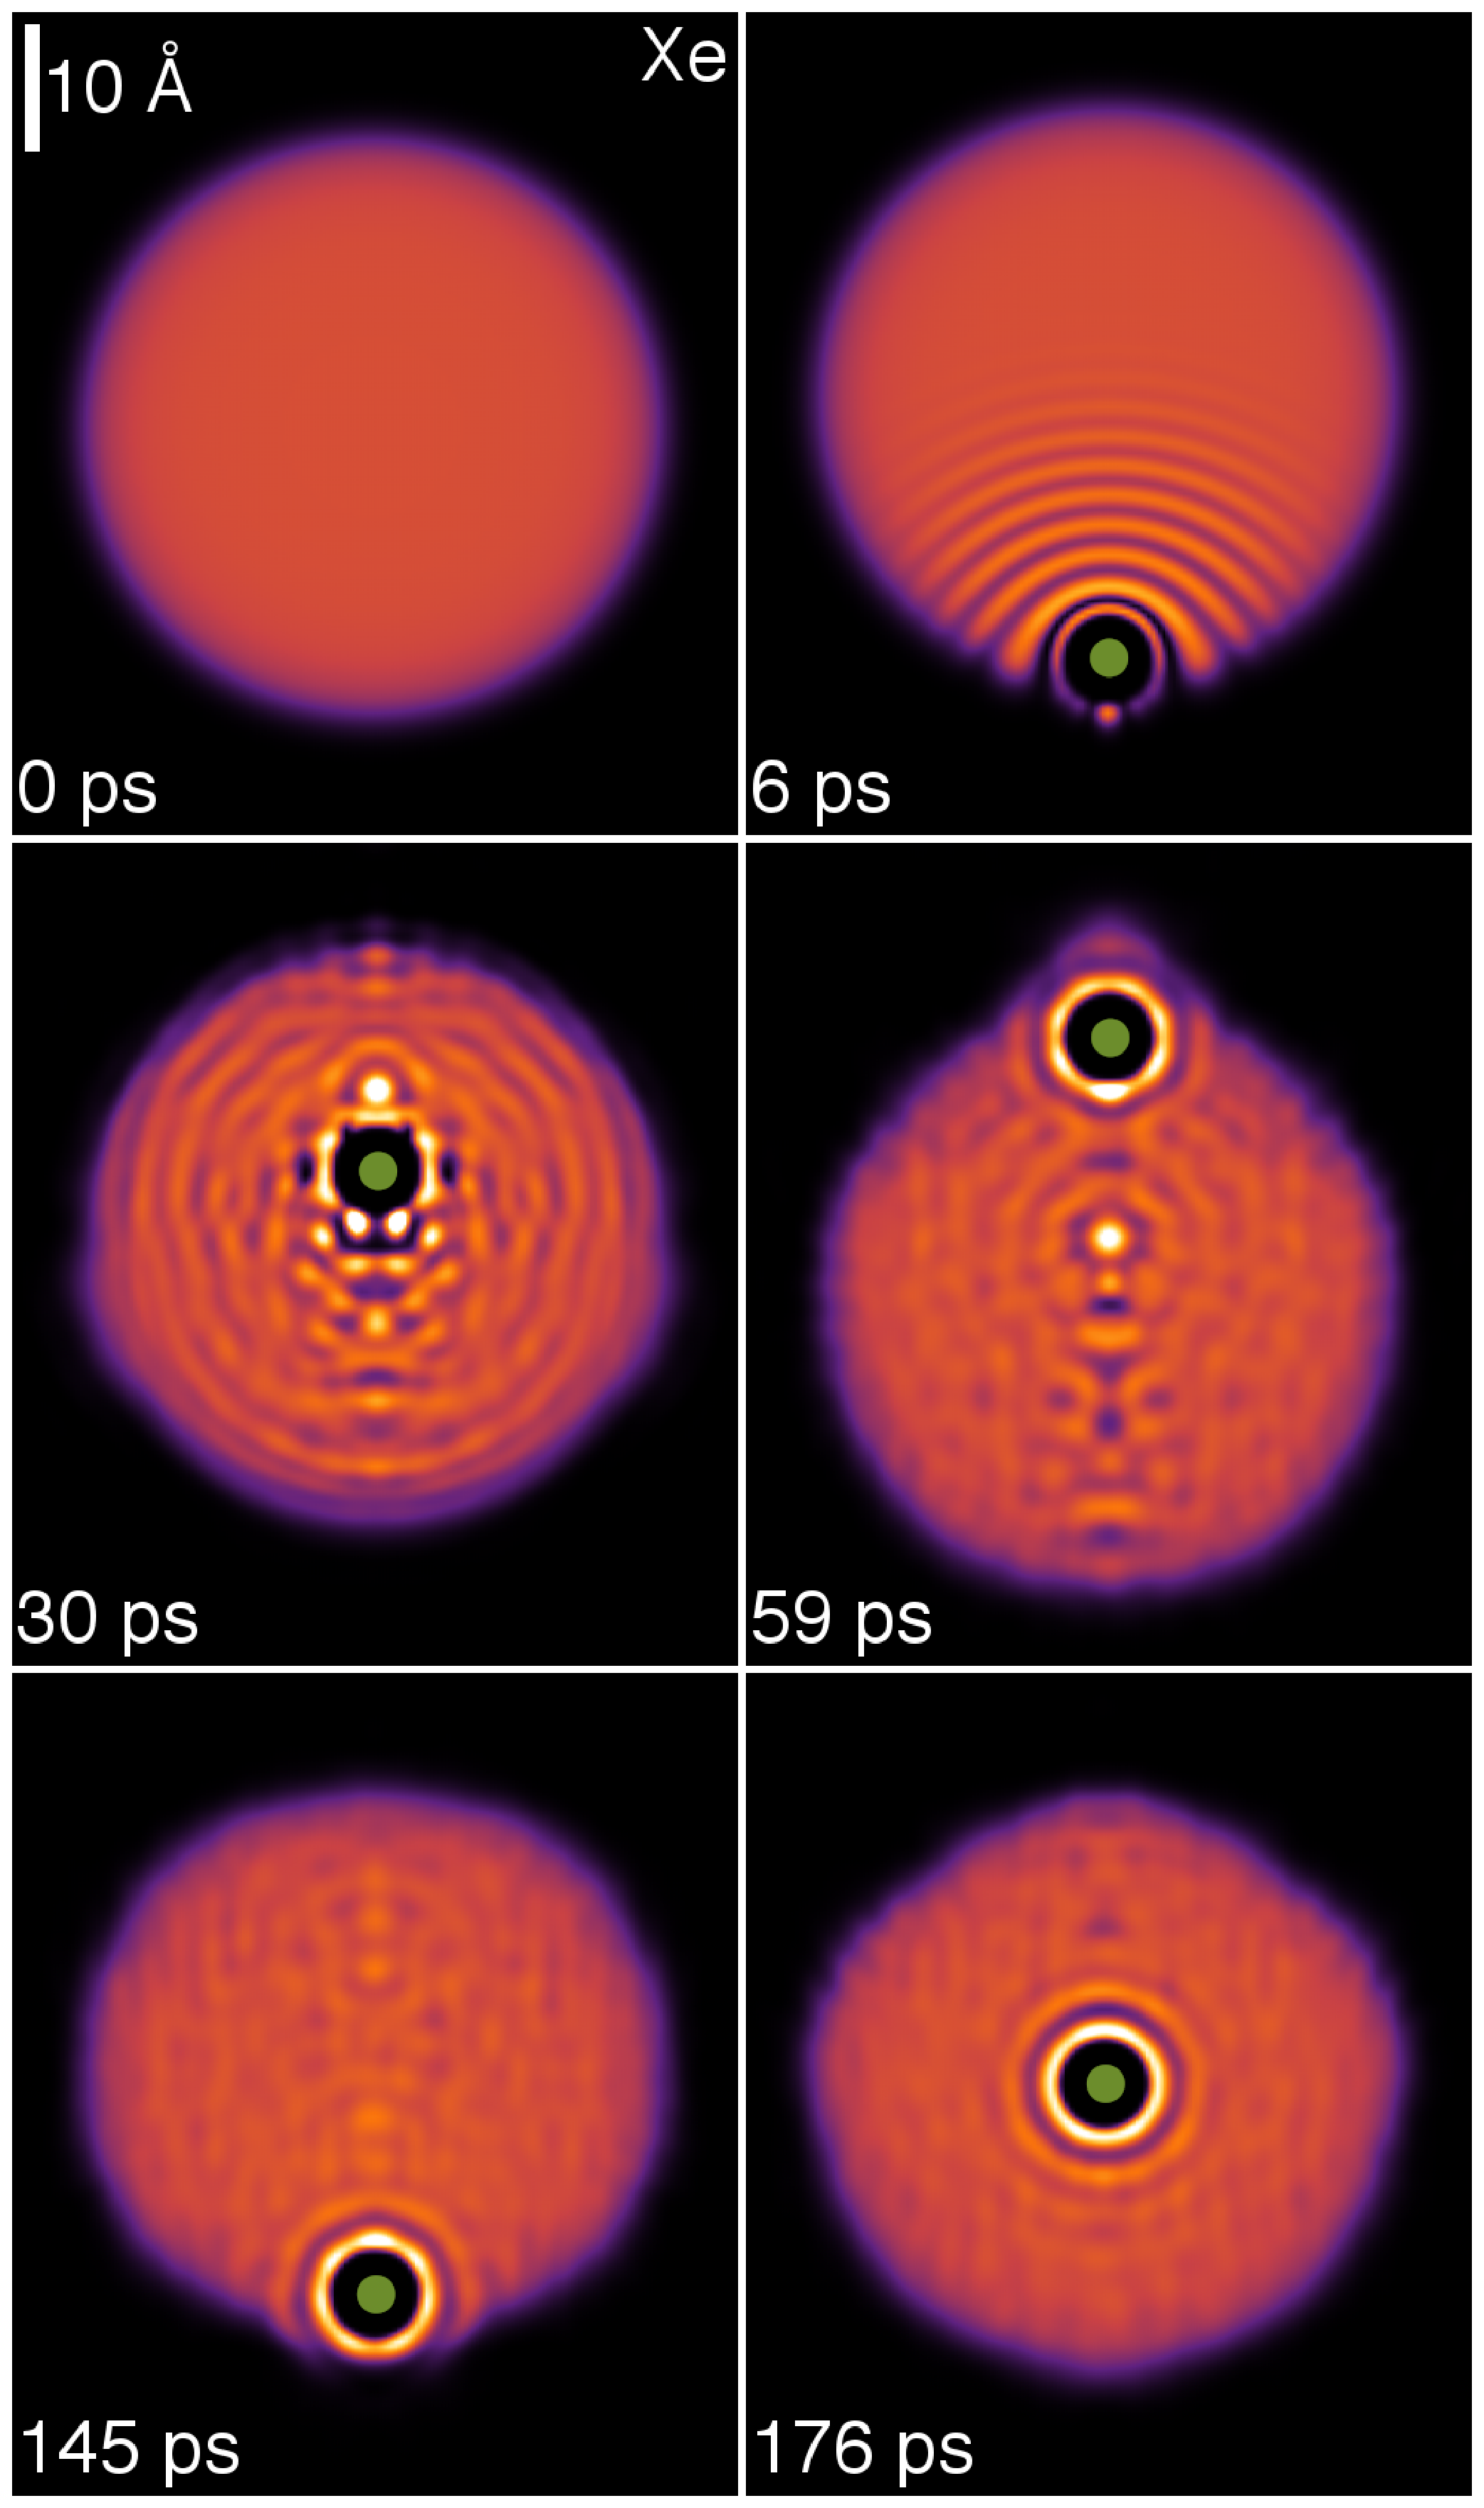
\includegraphics[width=0.50\linewidth,clip]{fig2-Xe}}
			\caption{\label{fig2-headon}Right panel: Dynamic evolution of a Xe atom (big dot) approaching the $^4$He$_{1000}$ droplet from below at $v_0 = 200$ m/s. The corresponding time is indicated in each frame. Left panel: Same as left figure for a Cs atom. (Color figure online.)}
		\end{figure}

		\begin{figure}[!]
			\centerline{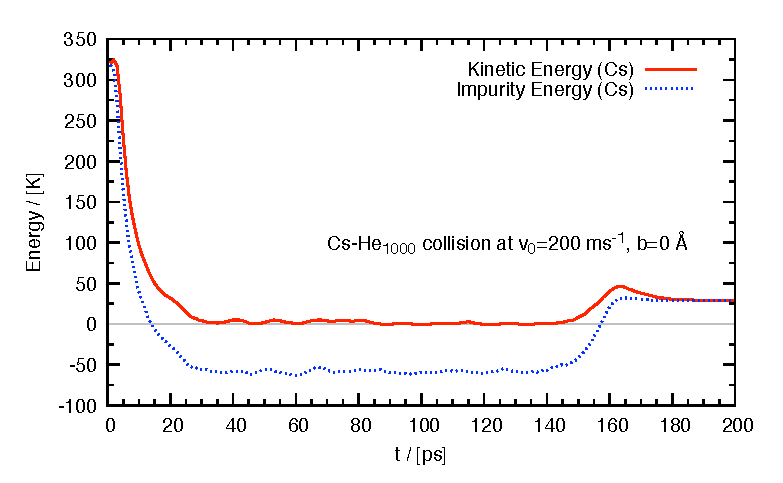
\includegraphics[width=0.90\linewidth,clip]{fig3-Cs-He}} 
			\centerline{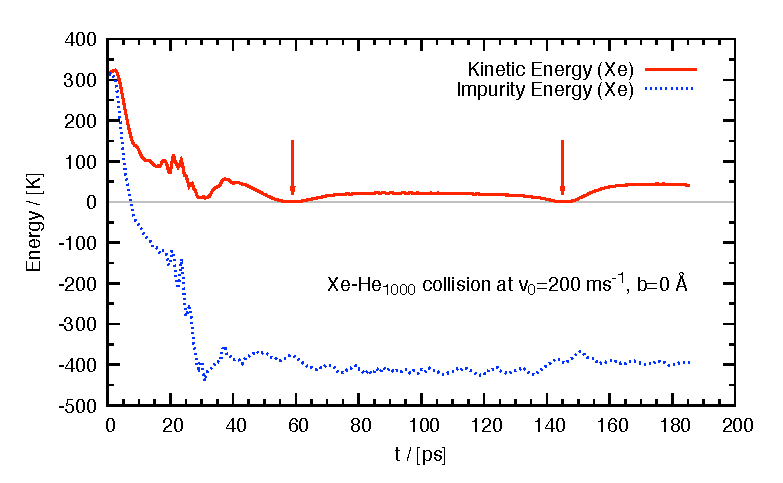
\includegraphics[width=0.90\linewidth,clip]{fig3-Xe-He}}
			\caption{\label{fig3-headon}Top figure: Kinetic and total (kinetic plus potential) energy as a function of time  of a Cs atom head-on colliding against a  $^4$He$_{1000}$ droplet at  $v_0 = 200$ m/s. Bottom figure: same as top figure for a Xe atom. The vertical arrows indicate the first two turning points at 59 and 145 ps, whose corresponding helium densities are shown in the right Fig. \ref{fig2-headon}. (Color figure online.)}
		\end{figure}

		We consider a droplet made of $N=1000$ helium atoms. Its ground state structure is obtained using DFT and gives a sharp-density  radius of about 22.2 \AA{}. Then the dynamics is initiated by placing the Xe atom 32 \AA{} away from the center of mass (COM) of the droplet with an impact parameter equal to zero (head-on collision). The simulations are carried out for initial Xe velocities  $v_0$ ranging from 200 to  600 m/s in the system of reference of the droplet, corresponding to kinetic energies between  315.8 K and  2842 K. These energies can be compared to the solvation energy of a Xe atom at the center of a $^4$He$_{1000}$ droplet, $S_{{\rm Xe}} = E({\rm Xe}@^4{\rm He}_{1000}) - E(^4{\rm He}_{1000}) = -316.3$ K. For the sake of comparison, the solvation energy of Cs is -5.2 K and its equilibrium position is  in a dimple at the outer droplet surface, about 26.6 \AA{} from its centre. 

		Thermal Xe atoms ($v_0 \sim$ 240 m/s) are used in the experiments \citep{Gom14,Jon16}, and the average drop velocity is about 170 m/s \citep{Gom11}.

		Figure \ref{fig1-headon} shows the energy of  the Xe@$^4$He$_{1000}$ complex  referred to that of the equilibrium configuration (Xe at the center of the droplet, $-5716.4$ K) as a function of the distance between the Xe  atom and  the COM of the droplet. It is obtained by a constrained calculation similar to that presented in Ref. \citep{Lea16} for Ba$^+$. 
With increasing distance, the stretched droplet-Xe configuration eventually breaks into a minicluster around the Xe atom containing 
about 22 helium atoms disconnected from the rest of the droplet.
The appearance of this minicluster is at variance with the situation for a heliophobic impurity such as Cs \citep{Lea14}.
The stretched (connected) configuration energies are represented by dots, the disconnected ones by triangles.
The two corresponding curves cross at  37 \AA{}.
At shorter distances the connected configuration is stable and the disconnected one metastable, and at larger distances the roles are inverted.
In an actual dynamics the number of He atoms in the minicluster  depends on the velocity of the Xe projectile.

 Figure \ref{fig2-headon} displays two-dimensional plots of the helium density for Xe  head-on  colliding against the $^4$He$_{1000}$
 droplet at $v_0=$ 200 m/s, and Fig. \ref{fig3-headon} the energy of the impinging atom as a function of time,
 with the corresponding plots for Cs collisions for the sake of comparison.  It can be seen that for both species
 most of the initial kinetic energy is spent in piercing the droplet surface, after which the impurity moves inside the droplet  
at a velocity  well below the critical Landau velocity  $v_L$. 
 
Figure \ref{fig2-headon} also shows that the collision launches a series of density waves in the droplet 
  that are reflected at the droplet free surface producing  complex interference patterns in
 its bulk. As an illustrative example, Fig. \ref{fig4-headon} shows the density profile along the incident direction ($z$ axis) corresponding to the Xe collision at $v_0=$
 200 m/s, 6 ps after the process starts.
 The wave number  associated to this  wave can be estimated from the wavelength $\lambda$  of the 
  oscillations, $q = 2 \pi/\lambda \sim$ 2.7 \AA$^{-1}$.

\begin{figure}[!]
\centerline{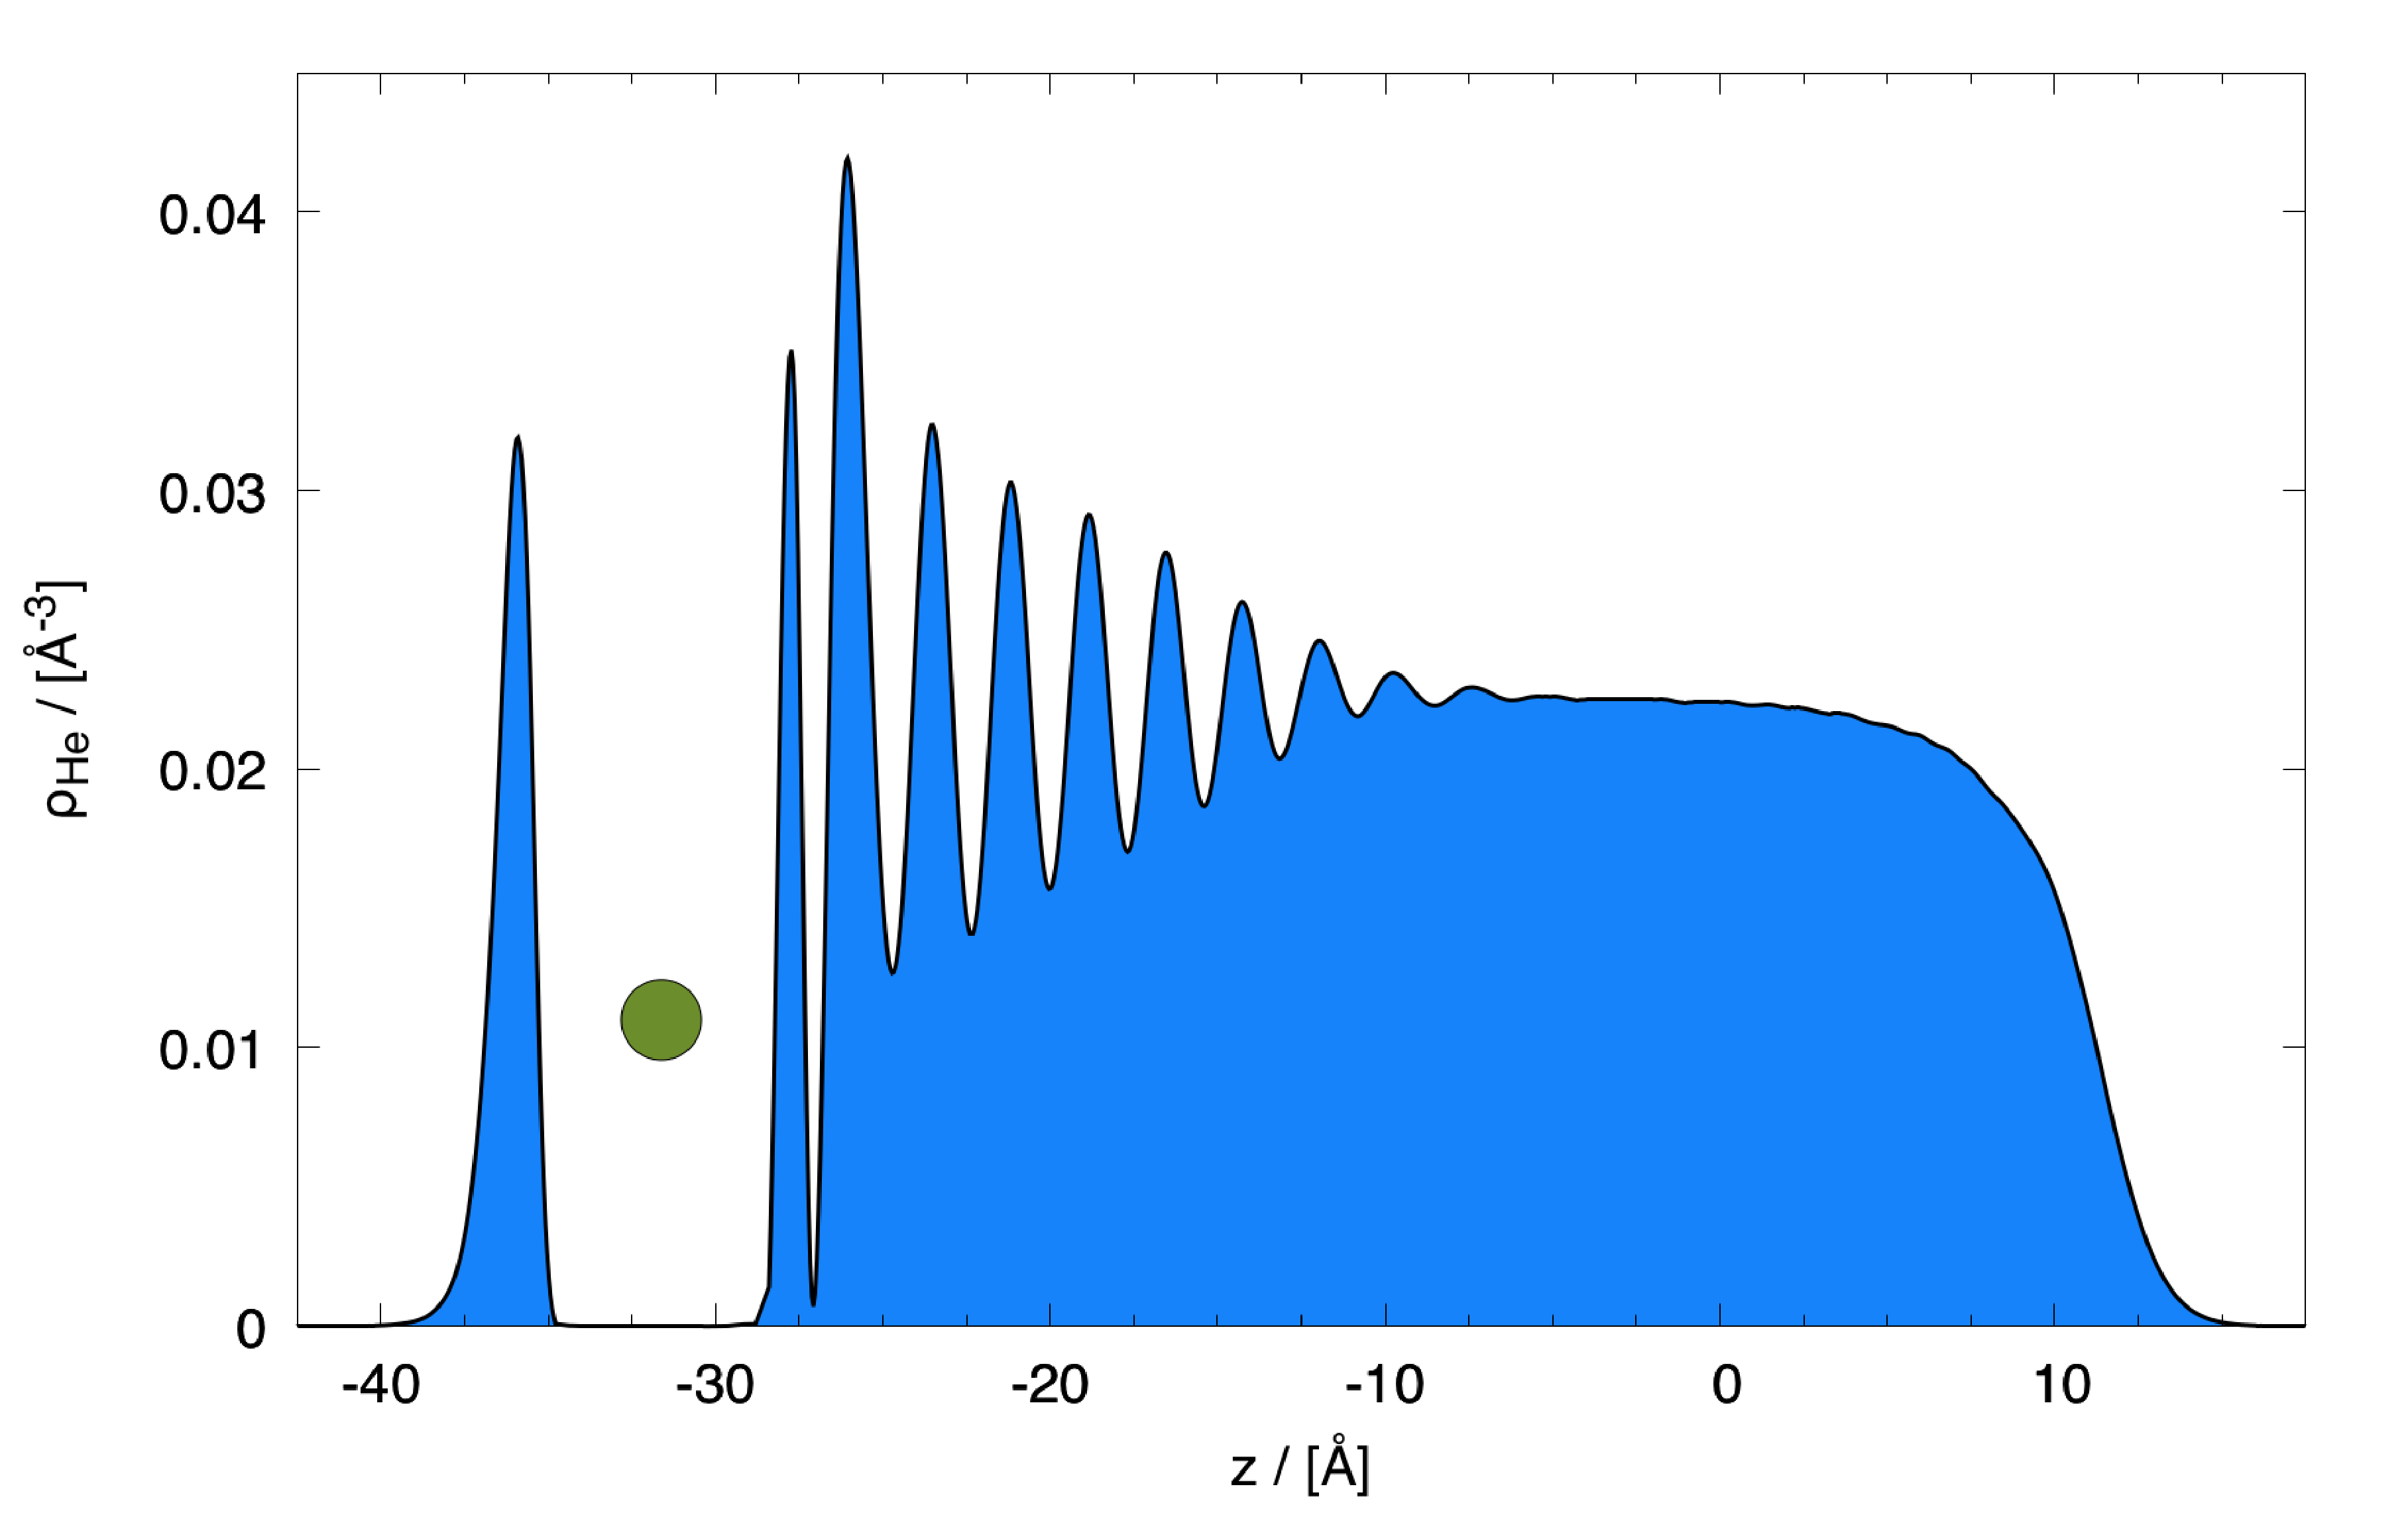
\includegraphics[width=0.90\linewidth,clip]{fig4}} 
\caption{\label{fig4-headon} 
Density profile of the He$_{1000}$ droplet along the incident direction corresponding to the Xe collision at $v_0=$
 200 m/s after 6 ps. (Color figure online.)
}
\end{figure}

In the case of Xe, Figs. \ref{fig2-headon} and \ref{fig3-headon}  reveal the appearance of turning points at which the velocity of the impurity is zero.
Note that these points are not fixed during the dynamics since the droplet deforms due to the swift motion of Xe inside it; 
the droplet is not a rigid object and reacts to the motion of the impurity, with  energy being transferred not only from the impurity 
to the droplet but also the other way around \citep{Mat14}.

The top left inset in Fig. \ref{fig1-headon} shows a snapshot obtained at the first turning point for $v_0=$ 600 m/s, with 57 He atoms around the Xe dopant.
We have found that the Xe atom has to hit the droplet at a velocity above 600 m/s  in order to go across the helium droplet, otherwise it remains attached to the droplet.
The kinetic energy lost by the Xe atom is partially deposited in the droplet and partially carried away by prompt-emitted helium atoms, \textit{i.e.} atoms expelled 
early on in the collision and with a significant kinetic energy. The number of He atoms 
 emitted during the first 78 ps is about 47. For comparison, about 19 atoms are emitted after 185 ps for $v_0$ = 200 m/s. 
 Eventually, the energy deposited into the droplet should be lost by atom evaporation; however, the time scale for this to happen is 
 beyond the reach of any realistic simulation. 
 
 
\begin{figure}[!]
\centerline{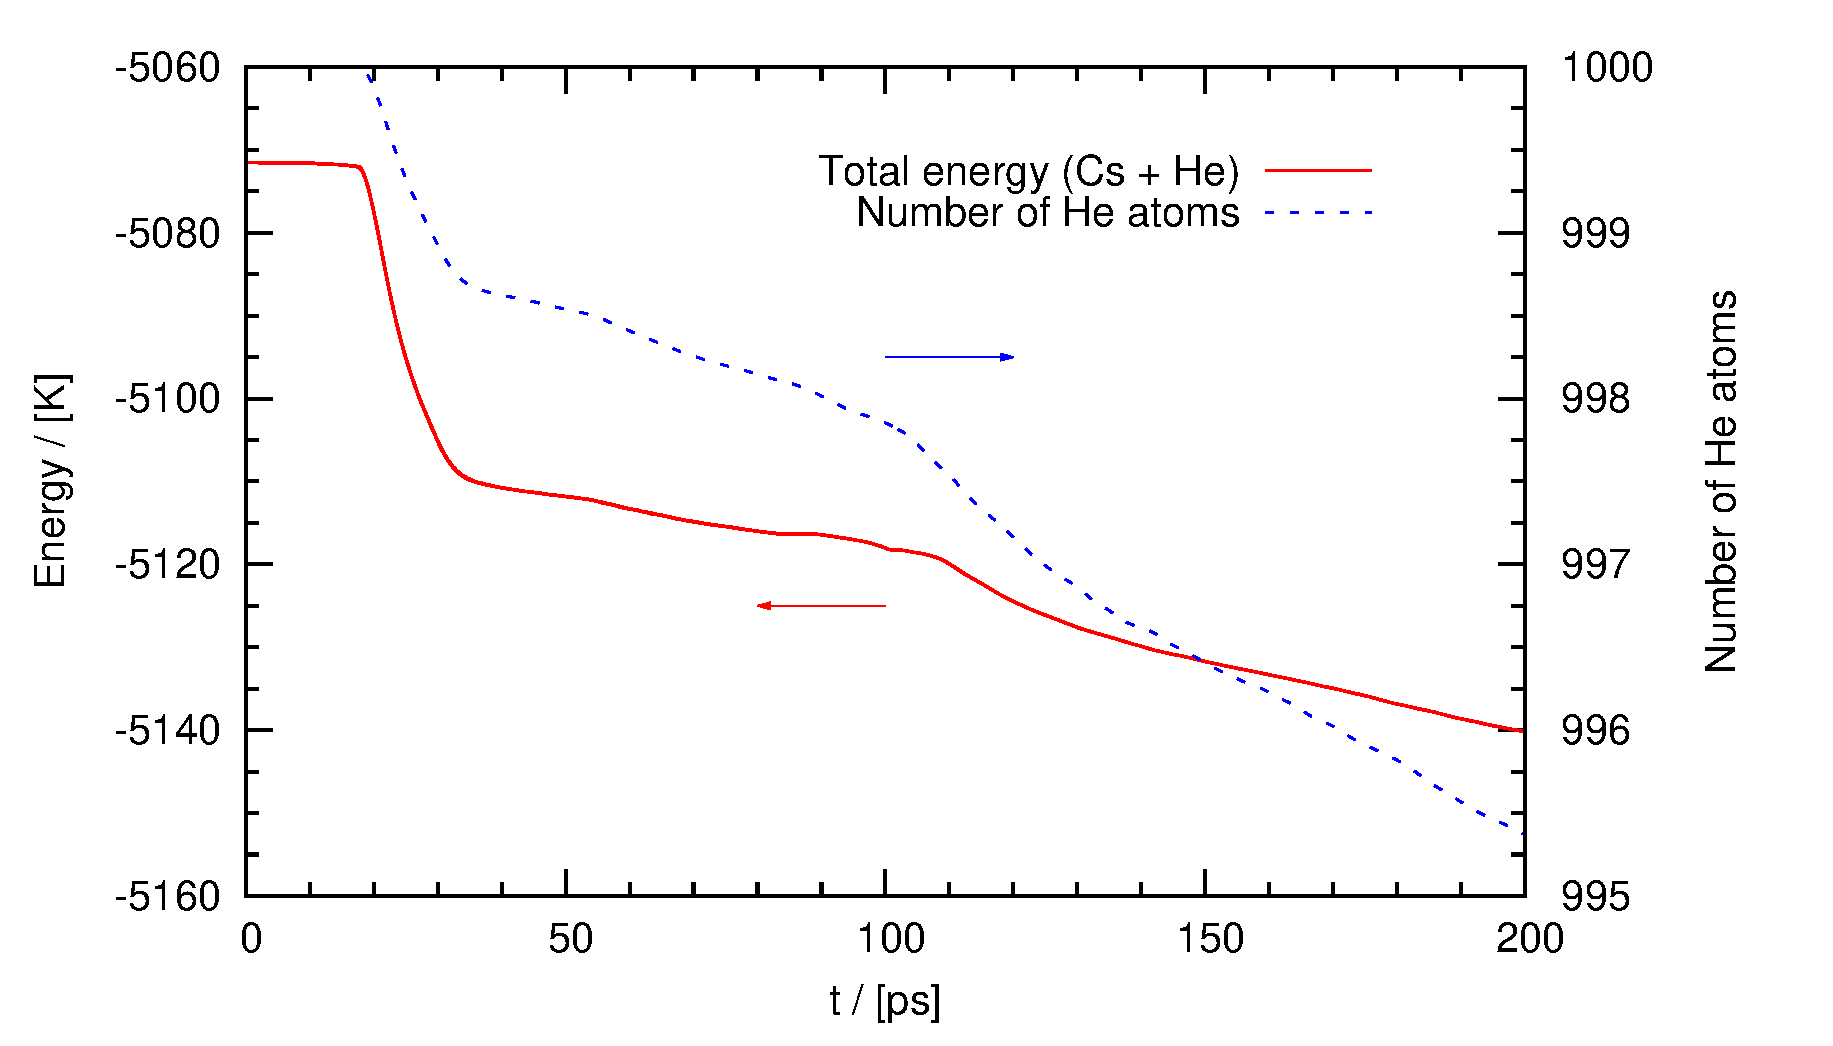
\includegraphics[width=0.90\linewidth,clip]{fig5}}
\caption{\label{fig5-headon} 
Total energy  (left scale) and number of atoms in the droplet (right scale) as a function of time for the 
Cs@$^4$He$_{1000}$ system at $v_0 = 200$ m/s. (Color figure online.)
}
\end{figure}

 
 The piercing of the droplet by the Cs atom produces a density wave that travels on its surface and collapses at the surface region opposite to the hitting point.
 This collapse nucleates a 
 vortex ring (the two dark spots in the 76 ps plot of the left panel of Fig. \ref{fig2-headon}) \citep{Lea14}.
 
 It is worth pointing out that the falloff of the Xe velocity in the $t=20-30$ ps interval observed in Fig. \ref{fig3-headon}  is due to the increase of its inertia
due to the appearance of a dynamic ``snowball''  --a crust of helium atoms surrounding the Xe bubble indicated by the bright spots in 
Fig. \ref{fig2-headon}-- that is eventually washed out at larger times.
At variance with our findings for Ba$^+$ \citep{Mat14}, vortex rings have not been nucleated in the case of Xe; in particular, we have checked that the two dark spots  in the 30 ps plot of the right panel of Fig. \ref{fig2-headon} for Xe do not correspond to a vortex ring. 

The collapse of the Cs bubble at the surface of the droplet some 150 ps after the process 
 gives back to the impurity part of the kinetic energy it has lost  in the 
 piercing of the droplet. The Cs atom is expelled at 64.5 m/s (corresponding to 33.6 K kinetic energy). 
The number of prompt-emitted helium atoms is 5, which is smaller than for Xe at the same collision energy (19 atoms).
As revealed by Fig. \ref{fig5-headon}, they are  preferentially emitted as a forward  burst  (first sharp drop around 20 ps in the number of atoms) and as a 
backward burst  (second sharp drop slightly after 100 ps).
		\chapter{Capture by quantised vortices}
	\section{Introduction}
		It is well established that helium droplets can readily capture in their interior almost any atom or molecule interacting with them, as first shown for the case of Ne atoms,\citep{Sch90} with the notable exception of alkali\citep{Sti96} and some alkaline-earth\citep{Her07} atoms. This property, together with the extremely low temperature $(T)$ achieved in helium droplets -- of the order of 0.4 K -- makes them the perfect ultracold and inert environment for hosting and studying isolated atoms and molecules, which is at the basis of current applications of helium droplets for spectroscopic studies of atoms and molecules. Besides, the superfluid nature of helium facilitates binary encounters of atoms/molecules in the bulk of the droplet while absorbing the energy released upon recombination, making possible chemical reactions which would not otherwise occur in the gas phase. These unique properties  of helium droplets have had a huge impact on their study.\citep{Toe04,Sti06,Tig07,Cal11a,Mud14}

		The pickup of Ar, Kr and Xe atoms in the gas phase by $^4$He$_N$ droplets with $N> 10^3$ atoms produced by nozzle beam expansions was described about twenty years ago by Toennies and coworkers.\citep{Lew95} In these experiments the droplets in the helium beam were deflected by impacting with a secondary beam made of rare gas atoms. 

		Recently, a technique has been introduced to determine the size of large He droplets ($N> 10^5$). It is based on the attenuation of a continuous droplet beam through collisions with Ar atoms at room temperature.\citep{Gom11} The pickup chamber of the droplet beam apparatus is filled with argon gas and the helium droplets experience multiple, isotropic collisions with the Ar atoms on their way towards the detection chamber. 

		Large helium droplets could also be doped in this way. This method, using Xe atoms, has been instrumental for detecting and imaging quantized vortex arrays in helium droplets.\citep{Gom14,Jon16} Xe atoms were used in these experiments because of their large sensitivity to the x-ray coherent diffractive imaging employed to detect them within the helium droplets. Experiments with large superfluid helium droplets are reviewed in a recent publication.\citep{Tan17}

		The impurity-droplet interaction in the presence of vortices is also relevant as the first stage of a more complex process leading to the formation of nanowires, see e.g. Refs. \citen{Lebedev2011,Gom12,Lat14,Tha14}. Long filaments made of micrometer-sized solid hydrogen particles trapped on quantized vortex cores were used to directly image the vortex reconnection between quantized vortices in superfluid helium\citep{Bewley2008}.

		The impact and capture of impurities interacting with pure helium droplets has been addressed recently within time-dependent density functional theory (TDDFT).
Real time simulations have been carried out for 
heliophobic\citep{Lea14a} (Cs) and heliophilic\citep{Vil16b} (Ne) atoms. In addition to the 
TDDFT equation for $^4$He, heavy impurities are treated as 
classical particles using
Newton's equation of motion, whereas a time-dependent 
Schr\"odinger equation has been used in the case of  
light impurities within the mean field model.\citep{Her12a,Vil16b}  
A comparison between the results for head-on collisions of Cs and Xe 
atoms --heliophobic and heliofilic atoms of similar mass-- has been presented in ref. \citep{Cop16}.

In this work we present results obtained within TDDFT 
for the collision and capture of Xe and Ar atoms by a $^4$He$_{1000}$ 
droplet at different kinetic energies and impact parameters. Special attention is paid 
to the  time-dependent interaction of Xe and Ar atoms with 
helium nanodroplets hosting 
vortex lines, and to the effect of multiply-doped vortex arrays in large helium droplets.

Due to the heavy computational cost 
of the TDDFT simulations presented here, 
we  address only a few facets of the capture 
process that we consider of experimental relevance
rather than carrying out a systematic study of the process. In particular:

$\bullet$ We study the capture of Xe atoms by a $^4$He nanodroplet, both for head-on 
collisions and for different impact parameters,
with velocities ranging from thermal values up to several hundred m/s.
The results of peripheral collisions  
with different values of the impact parameter 
are used to estimate the cross section for the
Xe capture.
 
$\bullet$ We study how a Xe atom dynamically interacts with a 
droplet hosting a vortex line, under different initial conditions
resulting in different velocity regimes of the impurity as it 
collides with the vortex core:
%(i) a Xe atom initially located in the interior of
%the droplet and close to the vortex core;
i) a Xe atom initially at rest on the droplet surface and
sinking under the effect of solvation forces;
(ii) a head-on collision of a moving Xe or Ar atom  against the
$^4$He nanodroplet.

$\bullet$ We study the stationary state of 
a large $^4$He$_{15000}$ 
droplet hosting a ring of six vortex lines, doped with 
Ar atoms completely filling all six vortex cores. This is the simplest system that mimics those
experimentally described in ref. \citep{Gom14}, where 
doped vortex arrays embedded in rotating $^4$He microdroplets have been imaged.
 
%$\bullet$ We address a
%vortex dipole configuration made of a vortex-antivortex pair in a pure $^4$He$_{1000}$ droplet, and the collision of a Xe atoms against it.
%Vortex dipole configurations appear  
%in  Bose-Einstein condensates (BEC) made of cold gases.\citep{Fre10}  
%At variance with 
%a configuration made of two vortices with equal rotation direction,
%in which the vortices turn around  each other in the laboratory frame,
%a vortex dipole is stationary. 

%In bulk liquid $^4$He the generation of pairs of linear vortices,
%with either the same or opposite sign, occurs 
%as a consequence of the motion of, e.g., a rigid wire 
%inside the liquid\citep{Anc17} in a geometry often employed 
%experimentally to study  quantum turbulence in 
%superfluid $^4$He.
%In helium droplets 
%the actual generation of vortex dipoles is
%rather unlikely. Yet it cannot  be discarded 
%that in the course of vortex array nucleation
%some antivortices are  also generated, temporarily coexisting with the vortex array. Addressing their stability and time evolution when the droplet captures an 
%impurity might thus have some interest.

Multimedia materials accompany this paper, 
showing the real time dynamics of several impact/capture processes 
described here. These materials  are presented 
in the electronic supplementary information (ESI$\dag$) document.
They constitute  an important part of this work, 
since often it is only by viewing how a complex microscopic process
unfolds in real time that one can catch important physical details 
which would otherwise escape in a written account. 

%\section{Theoretical approach} 
%
%The DFT model of liquid helium, 
%which describes the nuclear degrees of freedom quantum 
%mechanically, has emerged as the only 
%viable method to address the experimentally studied large 
%helium droplets. Its use constitutes a compromise between 
%the accuracy of ``ab initio'' methods (like Quantum Monte Carlo 
%methods\citep{Kro02}) and numerical feasibility.\citep{Bar06}
%Its essential features are recalled here for the sake of completeness.
% 
%Within DFT, the total energy $E$ of a $^4$He$_N$ droplet  
%at zero temperature is written as a functional of 
%the $^4$He atom density $\rho ({\mathbf r})$ 
%%
%\begin{equation}
%E[\rho] = T[\rho] + \int d{\mathbf r} \,{\cal E}_c[\rho]
%\label{eq1}
%\end{equation}
%where $T[\rho]$ is the kinetic energy of
%a fictitious system of non-interacting particles 
%(with mass $m_4$) constituting a BEC in the present case.
%
%As in recent applications of the TDDFT 
%approach,\citep{Her12a,Mat14,Van14,Lea14b,Lea16,Van17}  
%we use the correlation energy density functional 
%%{\cal E}_c
%${\cal E}_c$ 
%proposed in ref. \citep{Anc05a}. 
%This functional is finite-range and includes non-local effects.
%Both aspects are needed to describe
% the response of the liquid at the Angstr\"om-scale.
% Note that  a  zero-range 
% %reduction of the OT 
% density functional has been recently applied to the study of 
%inelastic scattering of xenon atoms by quantized 
%vortices in superfluid liquid $^4$He.\citep{Psh16}
%Particle-vortex collisions in thermal superfluid $^4$He have also been addressed.\citep{Kiv08}
%
%
%It is customary to define an order parameter $\Psi$ 
%(often called effective wave function) as
%$\Psi({\mathbf r}) = \sqrt{\rho ({\mathbf r})}$. The kinetic energy of the
%fictitious system of non-interacting particles is thus
%%
%\begin{equation}
%T[\rho] =
%\frac{\hbar^2}{2m_4} \int d {\mathbf r} |\nabla \Psi|^2
%\label{eq2}
%\end{equation}
%%
%Extension to time-dependent systems leads to 
%the following time-dependent equation
%%
%\begin{eqnarray}
%\imath \; \hbar  {\partial \over \partial t} \Psi({\mathbf r},t)&=& \left\{ -\frac{\hbar^2}{2m_4} \nabla^2 + \frac{\delta {\cal E}_c}{\delta \rho} \right\}\Psi({\mathbf r},t) 
%\nonumber
%\\
%& \equiv&
%{\cal H}[\rho] \,\Psi({\mathbf r},t) 
%\label{eq3}
%\end{eqnarray}
%%
%whose self-consistent solution provides the system density $\rho ({\mathbf r},t)=|\Psi ({\mathbf r},t)|^2$
%and hence its total energy $E$. If the effective wave function is written as
%$\Psi(\mathbf{r}, t)= \Phi(\mathbf{r}, t) \exp[\imath \,{\cal S}(\mathbf{r}, t) ]$, the particle current density is
%%
%\begin{eqnarray}
%{\mathbf j}({\mathbf r},t ) &=& - \frac{ \imath \; \hbar}{2 m_4} [\Psi^*({\mathbf r},t) \nabla \Psi({\mathbf r},t) - \Psi({\mathbf r},t) \nabla \Psi^*({\mathbf r},t)] 
%\nonumber
%\\
%&&= \frac{  \hbar}{ m_4} \rho({\mathbf r},t)  \nabla {\cal S}({\mathbf r},t)
%\end{eqnarray}
%%
% with $\rho ({\mathbf r},t)=|\Psi ({\mathbf r},t)|^2 = \Phi^2({\mathbf r},t)$. This allows to identify the velocity field 
% %
%$${\mathbf v}({\mathbf r},t) =   \frac{ \hbar}{m_4} \nabla {\cal S}(\mathbf{r},t) $$ 
%%
%that fulfills  
%%
%$$\nabla  \times {\mathbf v}({\mathbf r},t)  =  \frac{ \hbar}{m_4}  \nabla \times \nabla {\cal S}(\mathbf{r},t)=0$$ 
%%
%but in general 
%%
%$$\nabla  \cdot {\mathbf v}({\mathbf r},t)  =  \frac{ \hbar}{m_4}  \nabla \cdot \nabla {\cal S}(\mathbf{r},t) = \frac{ \hbar}{m_4} \Delta {\cal S}(\mathbf{r},t) \neq 0$$ 
%%
%Thus, in the  zero temperature DFT approach, liquid helium flows  irrotationally.  Liquid helium  is compressible, a property that -- at variance with simpler approaches --
% is taken into account in the DFT method. 
%
%In the case of stationary states,
%$\Psi({\mathbf r},t)=\Psi_0({\mathbf r})e^{i\mu_4 t/\hbar}$ 
%and Eq. (\ref{eq3})  becomes
%%
%\begin{equation}
%\left\{-\frac{\hbar^2}{2m_4} \nabla^2 + \frac{\delta {\cal E}_c}{\delta \rho}
%\right\}\Psi_0({\mathbf r}) 
%= \mu_4 \Psi_0({\mathbf r})
%\label{eq5}
%\end{equation}
%%
%where $\mu_4$ is the $^4$He chemical potential. 
%
%The effect of heavy impurities like Ar and 
%Xe atoms embedded inside He droplets is incorporated as an external field. 
%The impurity-droplet interaction is 
%described within the pairwise sum approximation  
%%
%\begin{equation}
%E[\rho] \rightarrow E[\rho] +  \int d {\mathbf r} \rho({\mathbf r}) V_X(|{\mathbf r} - {\mathbf r}_I|)  \; ,
%\label{eq6}
%\end{equation}
%%
%$V_X$ being the He-rare gas interaction potential from 
%ref. \citep{Tan86}, and ${\mathbf r}_I$ the location 
%of the impurity. The helium density is obtained  by solving the 
%Euler-Lagrange (EL) equation
%%
%\begin{equation}
%\left\{-\frac{\hbar^2}{2m_4} \nabla^2 + \frac{\delta {\cal E}_c}{\delta \rho}  + V_X(|{\mathbf r} - {\mathbf r}_I|) \right\}\Psi_0({\mathbf r})  
%= \mu_4 \Psi_0({\mathbf r})
%\label{eq7}
%\end{equation}
%
%This static DFT equation is solved by the imaginary time method in cartesian coordinates. 
%The calculation is full 3D with no {\it a priori} imposed symmetry.
%A key tool for the implementation of the method is the use of 
%fast-Fourier techniques (FFT)\citep{Fri05} to calculate the convolutions needed to
%obtain some of the contributions to the total energy of the 
%impurity-droplet complex and the mean field potentials appearing
%in the EL equations.
%Densities, wave functions and differential operators are discretized on a cartesian grid. The 
%spatial grid intervals most often used in the applications are in the $0.3-0.4$~\AA{} range.
%The differential operators (first and second derivatives) are represented by 13-point formulas. 
%
%Once the static configuration has been obtained for a given impurity,  
%the dynamics starts by imparting a velocity 
%$\mathbf{v}_0$ to the impurity, initially 
%placed at a chosen location $\mathbf{r}_{I_0}$.
% $\Psi(\mathbf{r}, t)$ is thus evolved following the TDDFT 
%prescription and $\mathbf{r}_I(t)$ according to Newton's equation of motion:
%%
%\begin{eqnarray}
%\imath \; \hbar\frac{\partial}{\partial t} \Psi(\mathbf{r}, t)
%&=&
%\left[
%  -\frac{\hbar^2}{2m_4} \nabla^2 +
%  \frac{\delta {\cal E}_c}{\delta \rho}
%  +
%  V_{X}(|\mathbf{r}- \mathbf{r}_I|)
%\right]
%\Psi(\mathbf{r}, t)
%\nonumber
%\\
%m_I \ddot{\mathbf{r}}_I
%&=&
%-  \int d \mathbf{r} \, V_{X}(|\mathbf{r}- \mathbf{r}_I|)  \, \nabla \rho(\mathbf{r},t) 
% \; .
%\label{eq8}
%\end{eqnarray}
%%
%
%Equations (\ref{eq8}) are solved 
%using Hamming's predictor-modifier-corrector method\citep{Ral60}
%using the same box and grid as for the static problem. 
%In most cases, we have employed a time step of $\sim 0.5$ fs. 
%Hamming's method is not self-starting and requires the evaluation of 
%the solution for a few initial time steps. They were obtained using a 
%fourth-order Runge-Kutta-Gill algorithm.\citep{Ral60}
%
%During the time evolution some helium can be ejected off the droplet,  
%eventually reaching the boundaries of the cell used in the simulations. 
%If no action is taken this material will re-enter the simulation cell
%from the other side (periodic boundary conditions are implied in
%our calculations due to the use of FFT), therefore
% spoiling the calculation. We have
%handled this problem by including an absorption potential
%into the time-dependent equation for helium.\citep{Mat11a}
%Note that this particle --and thus energy-- leaking is physical: 
%it represents  helium atoms leaving the droplet and carrying away energy,
%although in a continuous way inherent to  the  DFT approach. 

\section{Results}

The results presented in this work have been obtained using the  4He-DFT BCN-TLS computing package\citep{Pi2017}.

\subsection{Xe capture by vortex-free droplets}

\begin{figure}[!]
\centerline{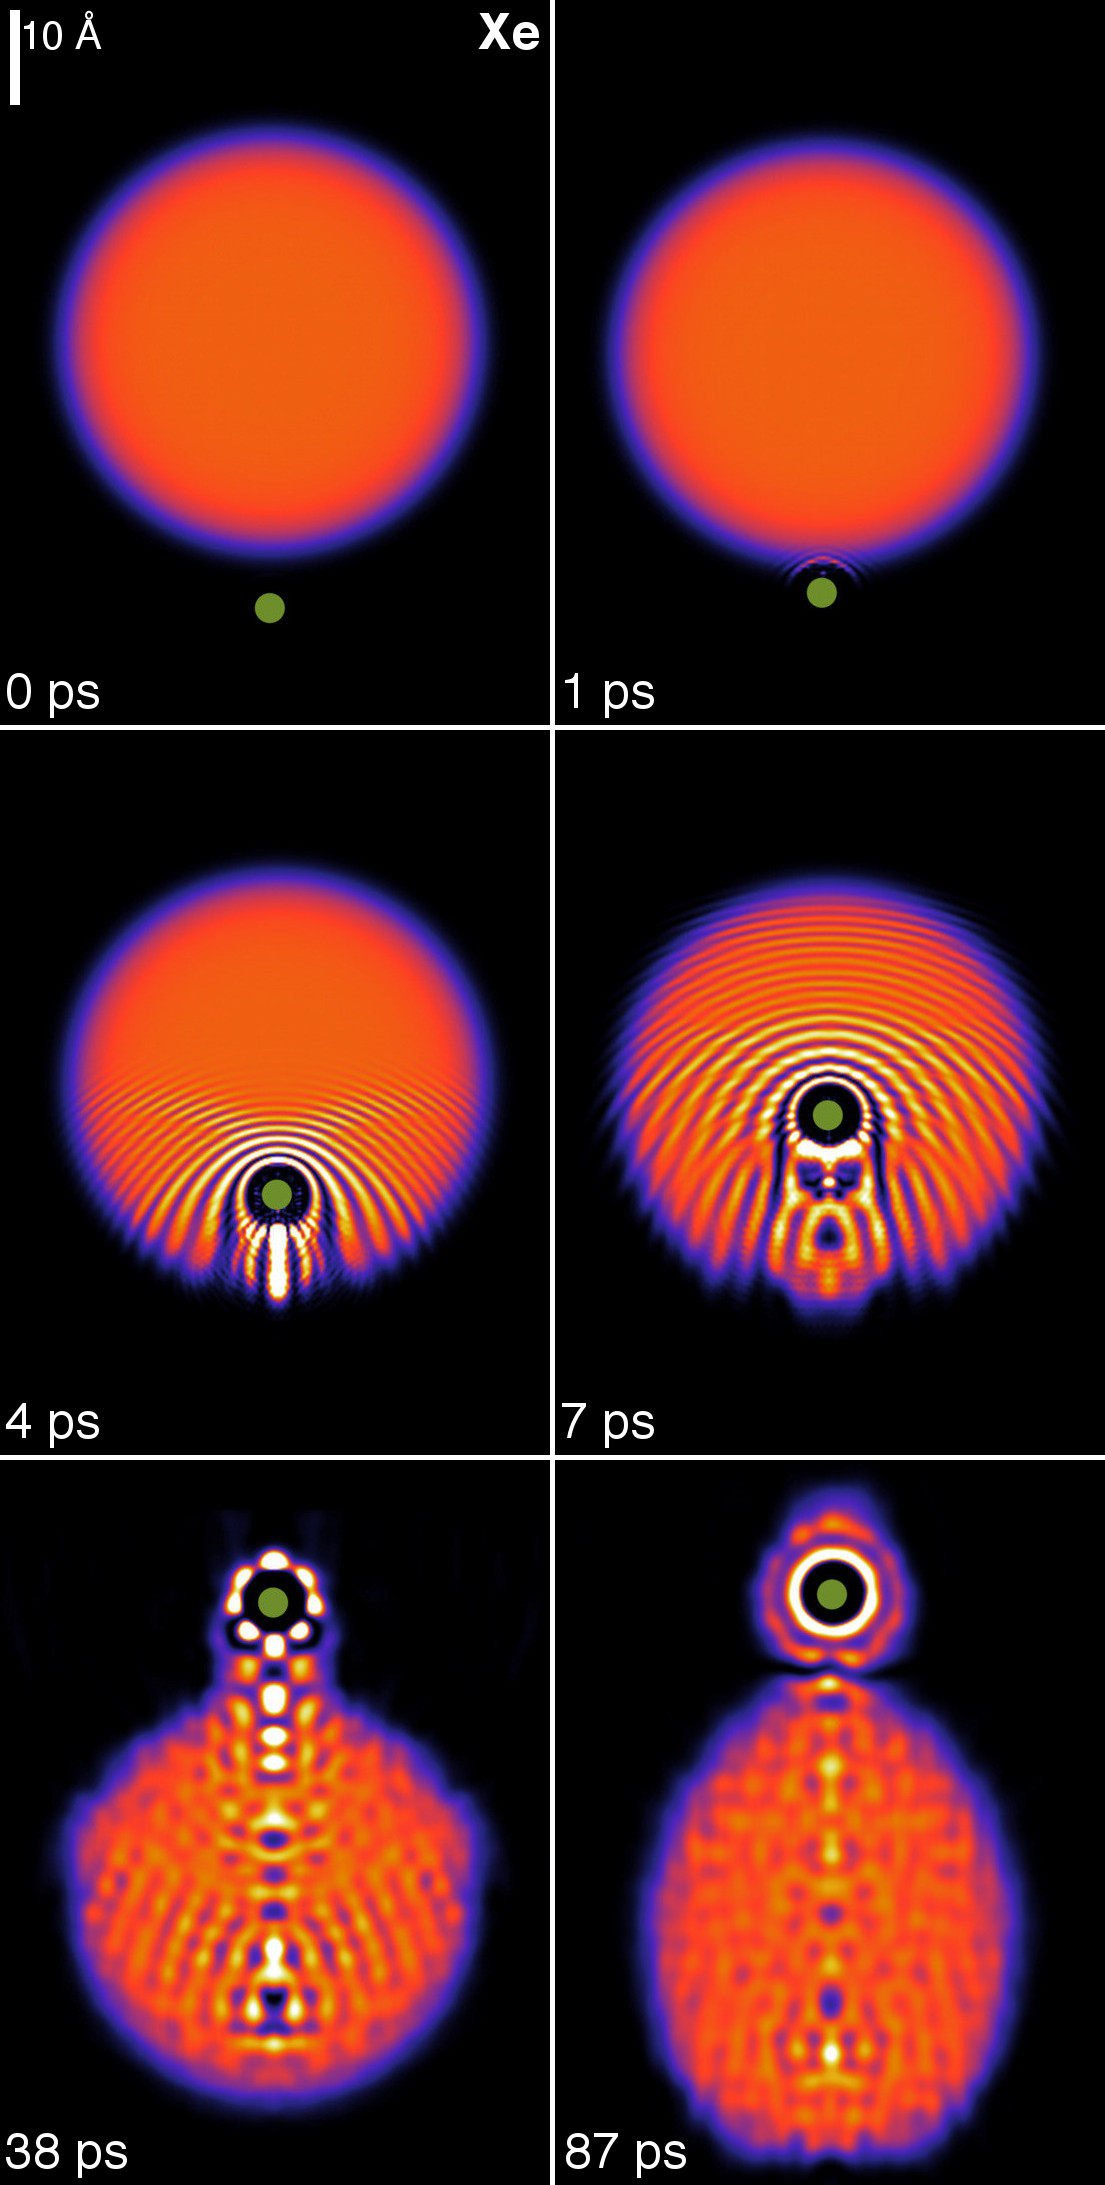
\includegraphics[width=0.6\linewidth,clip]{fig1-Xe-600mps}}
\caption{\label{fig1-capture} 
Dynamic evolution of a Xe atom (green dot) approaching the $^4$He$_{1000}$ 
droplet from below at $v_0 = 600$ m/s. The corresponding time is indicated in each frame. 
Bright spots correspond to high density regions.\citep{ESI} 
}
\end{figure}
%

\begin{figure}[!]
\centerline{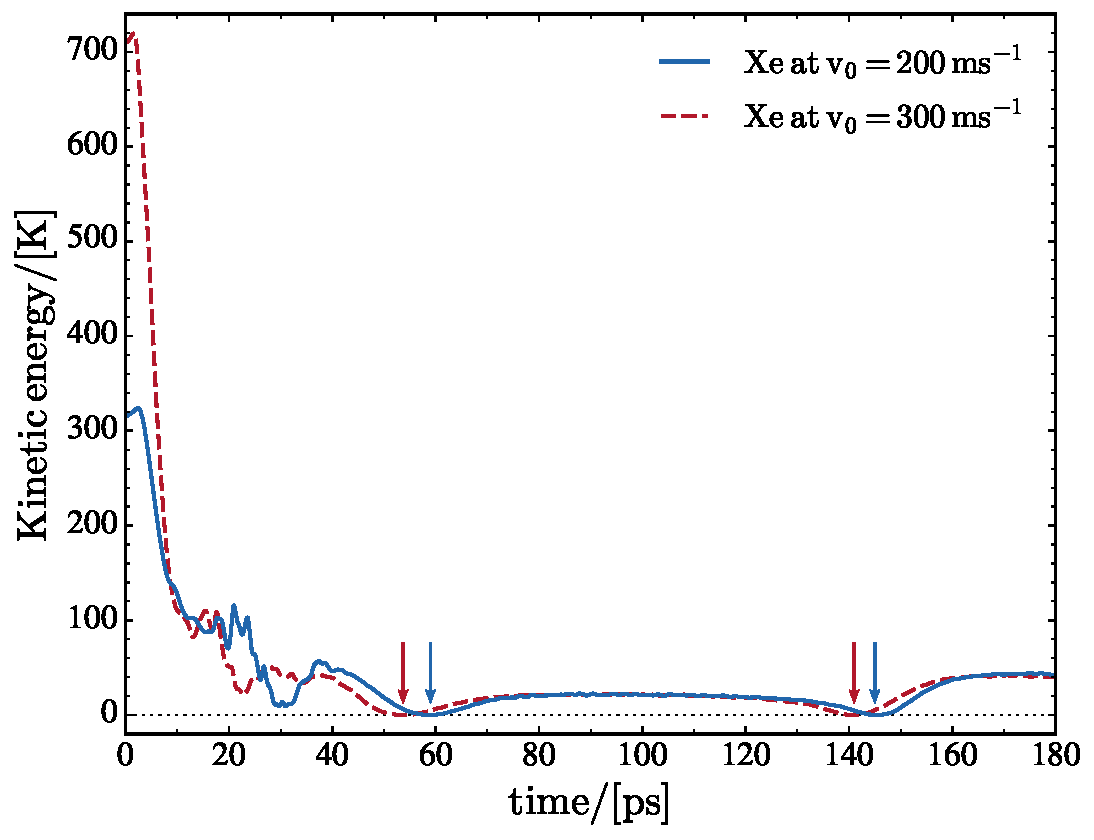
\includegraphics[width=0.9\linewidth,clip]{kinetic-energy}}
\caption{\label{fig2-capture} 
Kinetic  energy  of the Xe atom in the center of mass (COM) frame of the $^4$He$_{1000}$ droplet 
as a function of time for  a head-on collision  at $v_0$= 200 and 300 m/s. The kinetic energy increase 
during the first few picoseconds is due to the
acceleration produced by the attractive part of the Xe-He potential. The vertical arrows indicate the first two turning points inside the droplet.
}
\end{figure}
%
\begin{figure}[!]
\centerline{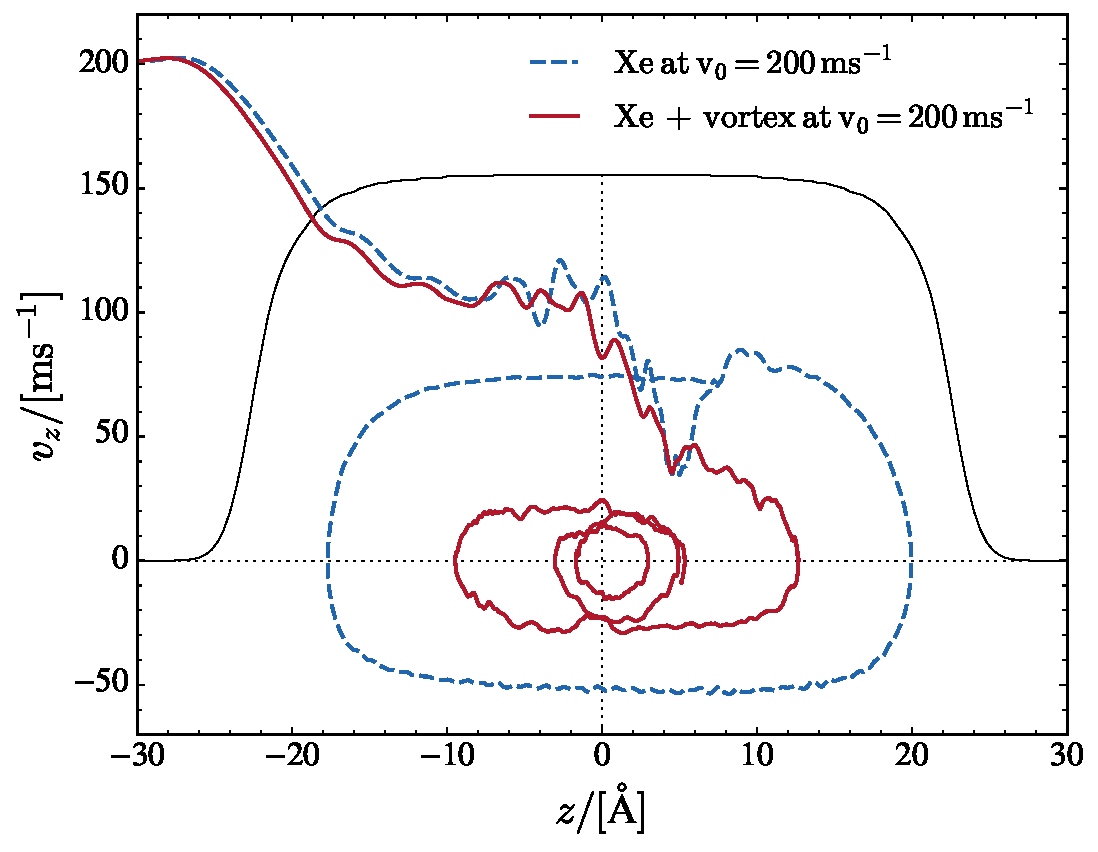
\includegraphics[width=0.9\linewidth,clip]{phase-Xe-200-vortex}}
\centerline{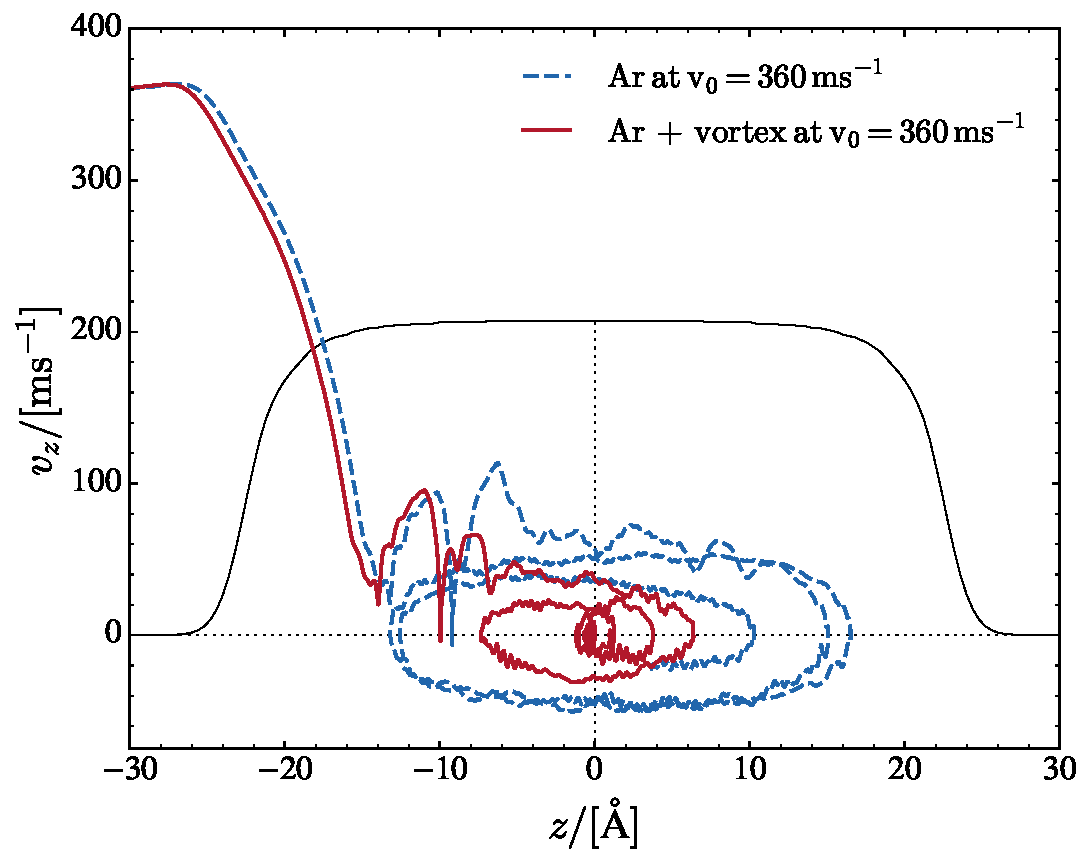
\includegraphics[width=0.9\linewidth,clip]{phase-Ar-360-vortex}}
\caption{\label{fig3-capture} 
Top: Phase-space trajectory  of Xe  for a  head-on collision at $v_0= 200$  m/s against a $^4$He$_{1000}$ droplet with and without a vortex line. 
The Xe atom is referred to the COM frame of the droplet.
Bottom: Same as top panel for Ar at $v_0=360$ m/s.
The droplet  density at $t=0$ is also represented in arbitrary scale (black profile) 
}
\end{figure}
%

%
\begin{figure}[!]
\centerline{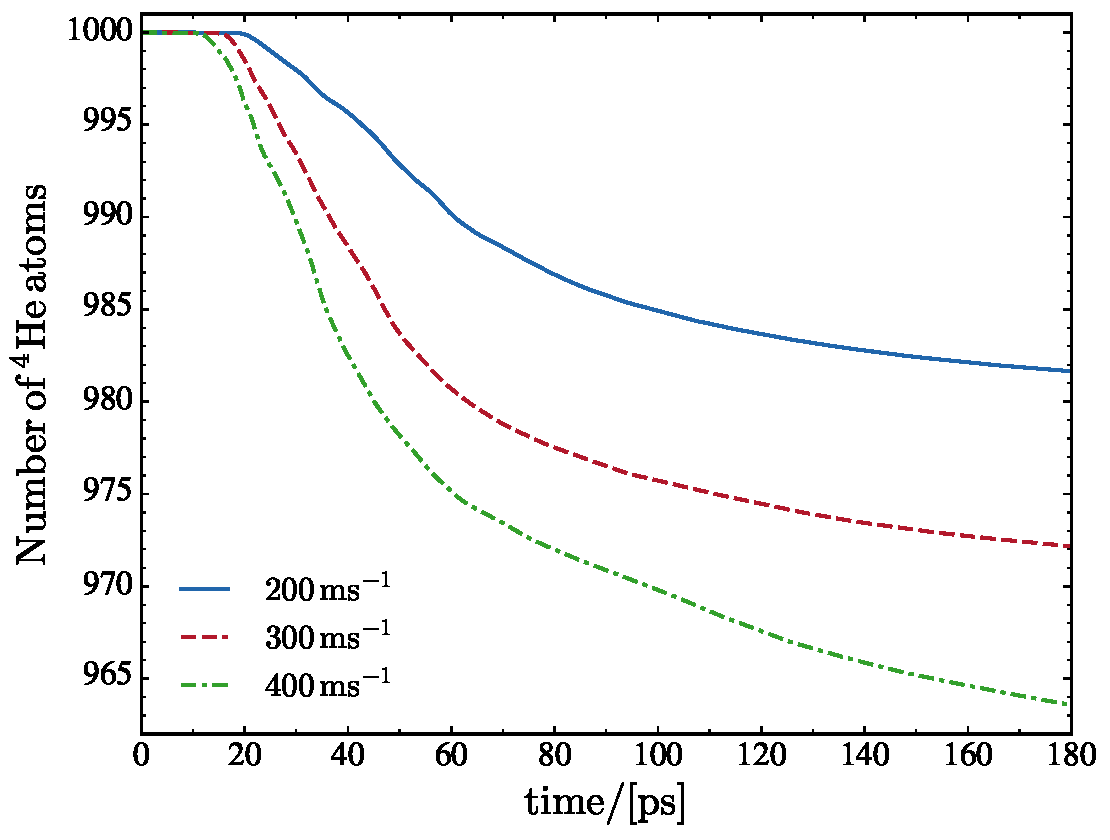
\includegraphics[width=0.9\linewidth,clip]{nparticles}}
\caption{\label{fig4-capture} 
Number of He atoms remaining in the droplet as a function of time for the
Xe against $^4$He$_{1000}$ collision at $v_0 = 200, 300$ and 400 m/s.
}
\end{figure}

We have simulated head-on collisions of a Xe atom with a
$^4$He$_{1000}$ droplet at relative velocities $v_0$ 
ranging from 200 to 600 m/s.  Figure \ref{fig1-capture} 
displays two-dimensional plots of the helium density 
for the highest value, $v_0= 600$ m/s. This velocity is 
well above the range of velocities typically encountered
in experiments.\citep{Gom11,Gom14,Jon16}  
In spite of the appearance of disconnected helium density shown in the 
$t= 87$ ps frame, we have found that the Xe atom eventually 
turns around and is 
captured again inside the droplet even at that relatively high impact velocity. 
Note that the Xe impurity, even when it temporarily emerges from the bulk of the 
droplet, appears to be coated with a few
$^4$He atoms, see the configuration at 87 ps.

Figure \ref{fig1-capture}  also shows the development of bow waves in the density profile, moving 
ahead of the impurity at 
supersonic velocity, and
an incipient  conic  density wave front  with its vertex at the Xe bubble.
Similar conic shapes, characteristic of supersonic flows, 
are found when an impurity moves in bulk liquid helium. 
In the present case the limited size of the droplet and 
the loss of kinetic energy
during the first stages of the collision
smooth out this front, making it just barely visible in the figure.

For low initial velocities of the impurity, we find that
Xe moves back and forth inside the droplet.
The turning points are not fixed,
because the droplet deforms due to the displacement 
of the Xe atom and to the waves that are continuously emitted 
by the moving impurity
(mainly in the direction of its  motion),
hit the droplet surface, and are reflected back inside it.\citep{Cop16}
This is shown in 
Fig. \ref{fig2-capture} for $v_0= 200$  and 300 m/s. 
Thermal Xe atoms ($v_0 \sim$ 240 m/s) 
are used in the vortex imaging 
experiments,\citep{Gom14,Jon16} and the average droplet velocity 
as it travels through the pick-up chamber is about 
170 m/s,\citep{Gom11} corresponding to relative collision
velocities which are within the range investigated here.
The kinetic energy gained by the Xe atom 
after the turning point at 140 --150 ps
is precisely due to the fact that the droplet is not a rigid 
object and reacts to the motion of the impurity.
As a consequence, energy is transferred not only from the impurity to 
the droplet but also the other way around. 
%A similar effect 
%was found in the sinking of a Ba$^+$ cation,
%see the multimedia view indicated in the caption of Fig. 2 of  ref. \citep{Mat14}
We want to emphasize that the droplet experiences 
large deformations rather than 
large displacements;
the velocity of the center of mass (COM) of the droplet is 
rather small (below 6 m/s  for $v_0= 200$ and 300 m/s as well) 
due to the large 
mass difference between the impurity and the droplet.

We have found that most of the energy is transferred from 
the Xe to the droplet in the first stages of the collision.
This is why, for collisions in this kinetic energy range 
leading to Xe capture, the motion of the impurity inside the droplet
is independent on the initial kinetic energy to a large extent.  
This is shown in Fig. \ref{fig3-capture}, which displays the trajectory
of Xe (Ar) in phase space for $v_0= 200$ (360) m/s. 
The figure also shows similar trajectories in the case where a vortex 
is present in the droplet; these cases will be discussed later in this paper.

%
% TABLE
%
\begin{table}[!]
\small
\caption{\label{tab1} Number of He atoms promptly ejected ($N_e$)  and average energy per ejected atom
($E_e$) during the first 200 ps. }
\vspace{0.1 cm}
\begin{tabular}{c c cc c c  c}
\hline 
%\hline
Species &\hspace{0.5 cm} & $v_0$ (m/s) &\hspace{0.5 cm}  & $N_e$ & \hspace{0.5 cm} & $E_e$  (K) \\
\hline
Xe  & &200 &  &18  & &19    \\
   && 300&  &28  &  &23   \\
   & &400 & &37 & &30 \\
   \hline
   Ar& & 360& & 16 & & 22 \\
\hline 
%\hline
\end{tabular}
 
\end{table}

The kinetic energy lost by the impurity atom is partly deposited 
in the droplet, where it produces large deformations and sound waves, 
and partly carried away by   prompt-emitted helium atoms. These are atoms  with a 
significant kinetic energy which are expelled from the droplet  
early on in the collision process. 
%A similar ejection appears in nuclear heavy ion reactions at intermediate energies, see e.g. ref. \citep{Ler85}
%and references therein.  
Fig. \ref{fig4-capture}   shows the number of atoms remaining in the simulation cell as a function of time
for collisions with Xe at $v_0= 200, 300 $ and 400 m/s. 
Eventually, the energy deposited into the droplet should be lost by atom evaporation.
The energy carried away by the ejected He atoms during the first 200 ps is 
collected in Table \ref{tab1} for the head-on collisions described in this paper.
For comparison, the  calculated binding energy of  a helium atom in the $^4$He$_{1000}$ droplet is $6.0$ K.
Note that helium atom ejection continues after 200 ps, the droplet still being far from ``thermalized'' (equilibrated).

In the case of heavy dopants it is possible to obtain 
a simple expression for their capture cross 
section.  Defining
%
\begin{equation}
\kappa=\sqrt{\frac{2 \mu E}{\hbar^2}} \;\; ,
\label{eq9}
\end{equation}
%
where $\mu$ is the reduced mass of the system and
$E$ is the available energy in the center-of-mass frame, and 
provided that the reduced de Broglie wave length of the impurity
$\lambda/(2 \pi) = 1/\kappa$ is much smaller than the dimensions 
of the droplet (which is the case for all $v_0$  in this study), the system
behaves classically and \citep{Lea14a}
%
\begin{equation}
\sigma(E)= \frac{\pi}{\kappa^2 } \sum_{\ell=0}^{\ell_{cr}} (2 \ell
+1)= \frac{\pi}{\kappa^2 } (\ell_{cr} +1)^2  
\label{eq10}
\end{equation}
%
where $\ell_{cr}$ is the largest relative angular momentum leading to the impurity capture. 
For a given energy, $\ell_{cr}$ is determined by 
carrying out simulations with different impact parameters $b$ using  
$\ell= \mu v_0 \, b/\hbar$.
We have done it for Xe at $v_0= 200$ m/s. Figure \ref{fig5-capture} shows the 
simulation corresponding to the largest impact parameter among the ones we have calculated
which led to Xe capture, $b=20.3$ \AA{}, and
Fig. \ref{fig6-capture} shows the simulation corresponding to the smallest one
which led to Xe deflection, $b=22.2$ \AA{}.
The radius of the 
droplet, which is defined as $R= r_0 N^{1/3}$ 
with $r_0 = 2.22$ \AA{}, is 22.2 \AA{} for $N=1000$. 
Hence, at this energy --well within the thermal conditions of the experiment--
the cross section for Xe capture is very similar to the geometric droplet cross section. 

 The circulation lines of the superflow are displayed 
in two selected panels in Figs. \ref{fig5-capture} and \ref{fig6-capture}. 
They show the flow  pointing towards
the approaching Xe atom at the beginning of the collision and the appearance of vortex loops  
in the droplet at the latest stages of the simulation.
Vortex loops appear  from local distortions of the droplet surface.\citep{Lea14b} 
%They have been found in other processes, such as the sinking of Cs$^+$ and Rb$^+$ cations in helium droplets.\citep{Lea14b}
%The motion of an impurity inside a droplet  has also been found to lead to vortex ring nucleation.\citep{Mat14} 
%It is unclear to us why sometimes  vortex rings are nucleated and sometimes not.
%We mention that 
The circulation lines  displayed  in the figures of this work have been drawn inside the region where the density is above  0.5 $\rho_0$ (with $\rho_0$= 0.0218 \AA$^{-3}$)
 that defines the dividing surface of the droplet. 

\begin{figure}[h]
\centerline{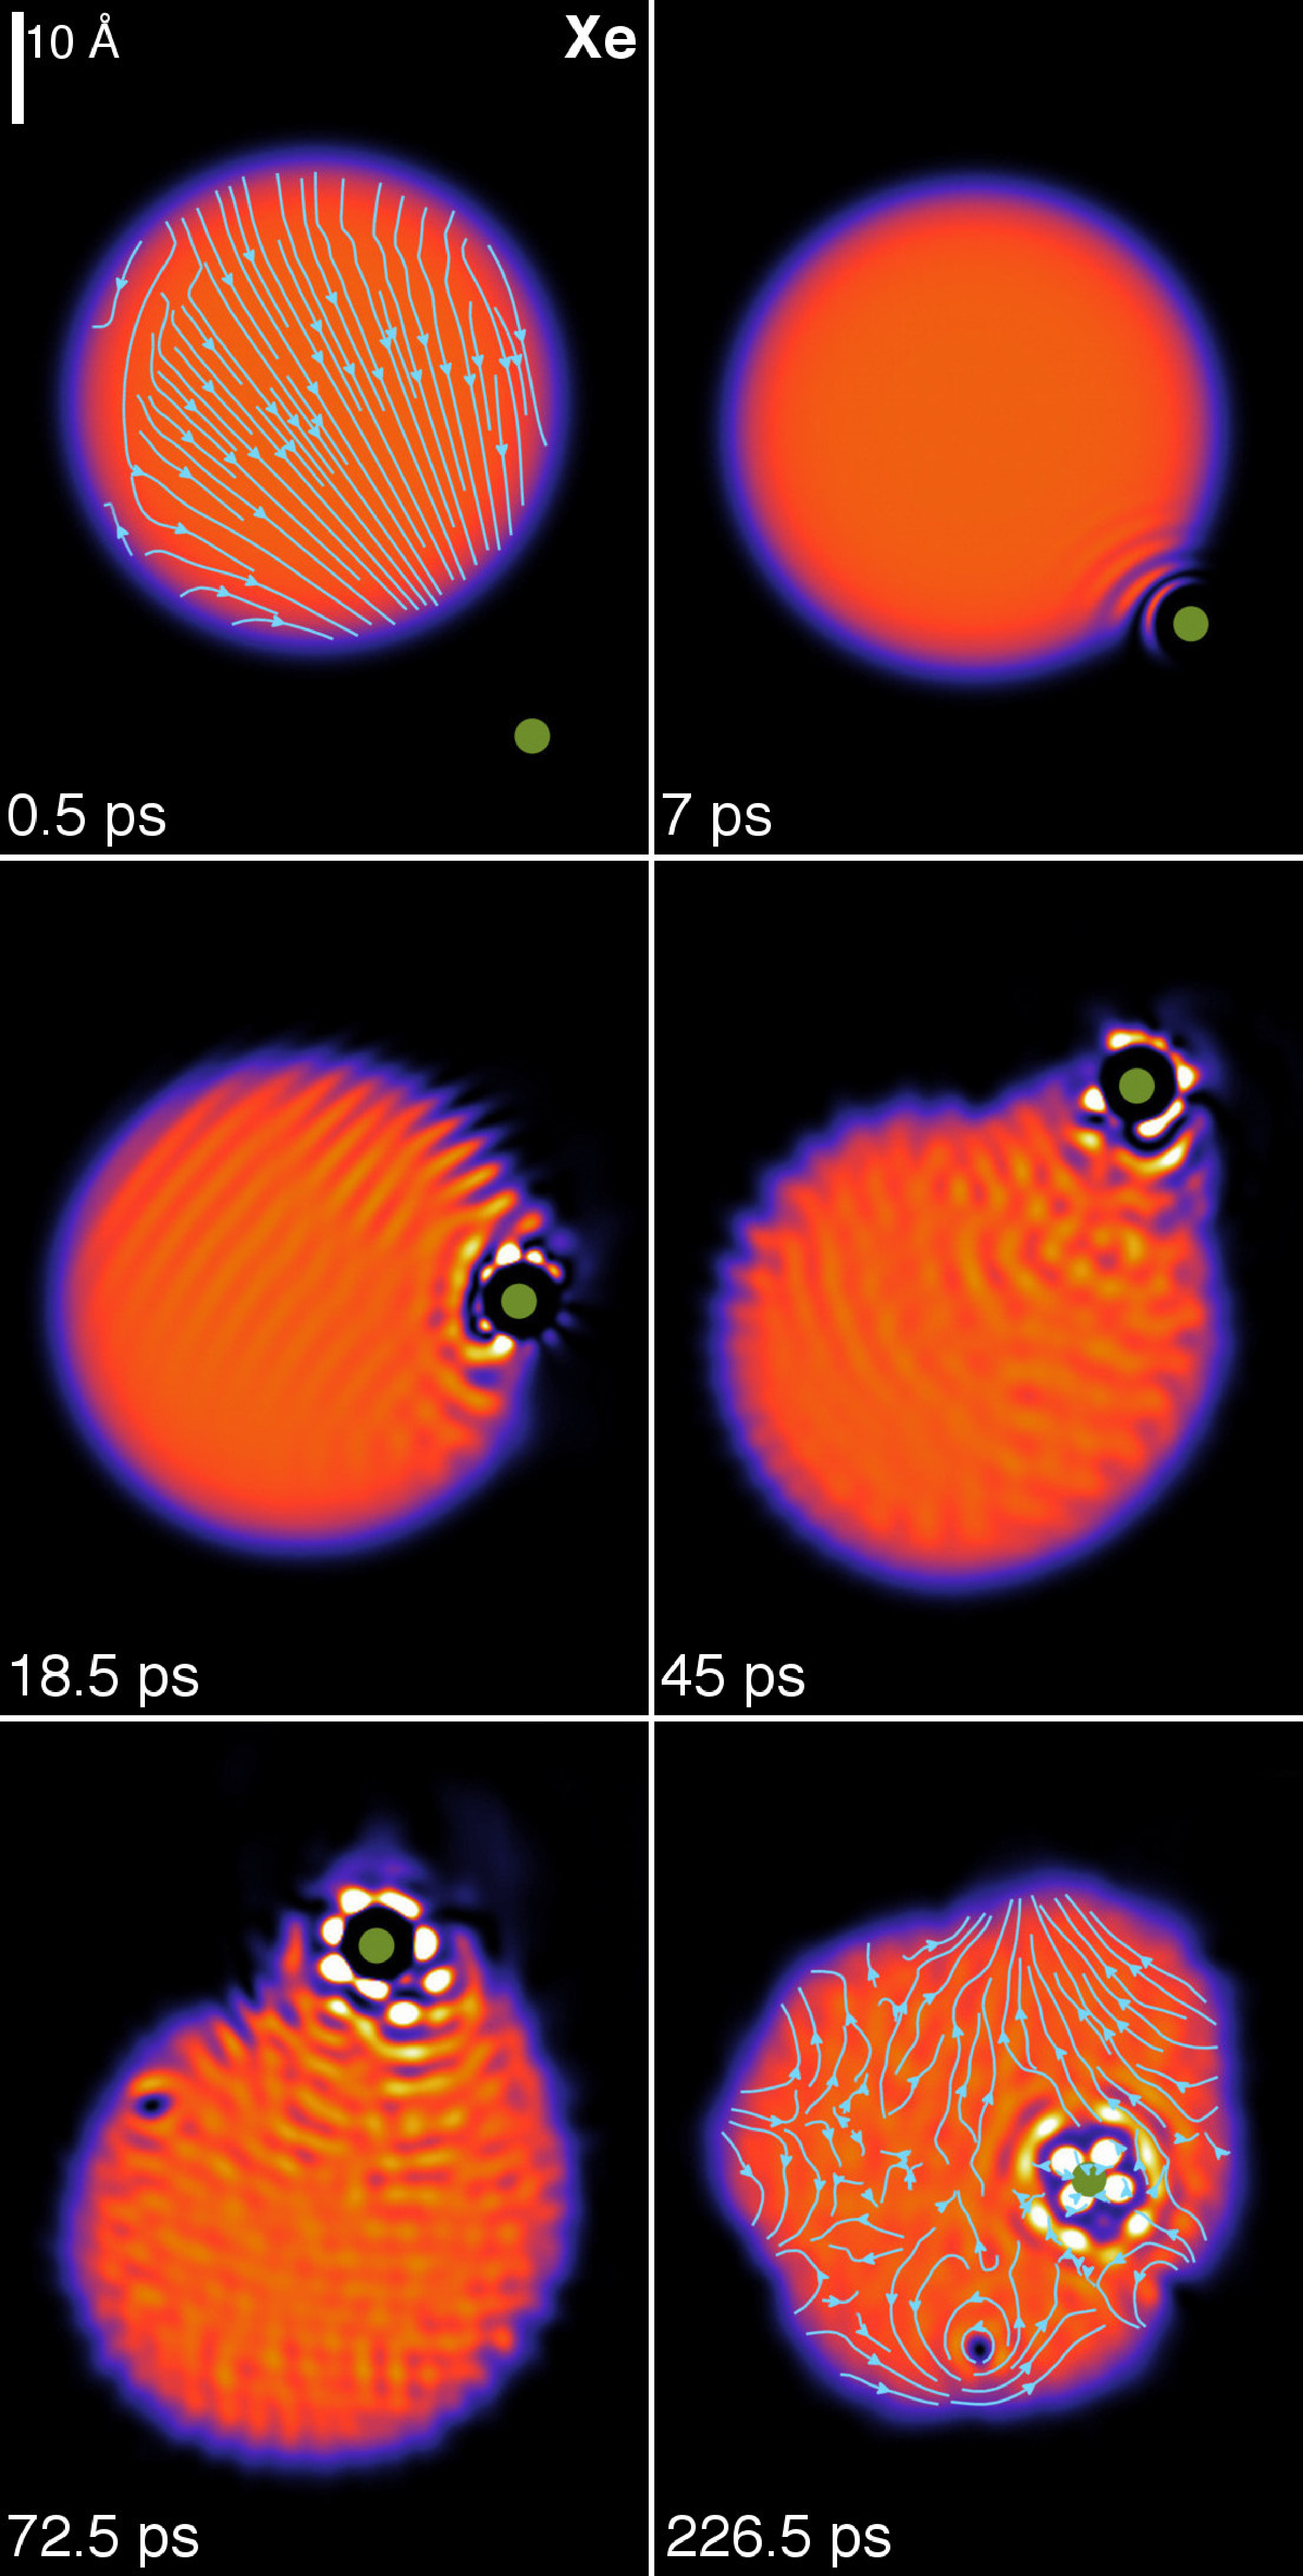
\includegraphics[width=0.60\linewidth,clip]{xehe200-b203-composed}}
\caption{\label{fig5-capture} 
Dynamic evolution of a Xe atom (green dot) approaching the $^4$He$_{1000}$ 
droplet from below at $v_0 = 200$ m/s with impact parameter $b = 20.3$ \AA{}. The corresponding time is indicated in each frame.\citep{ESI} 
}
\end{figure}
%

\begin{figure}[h]
\centerline{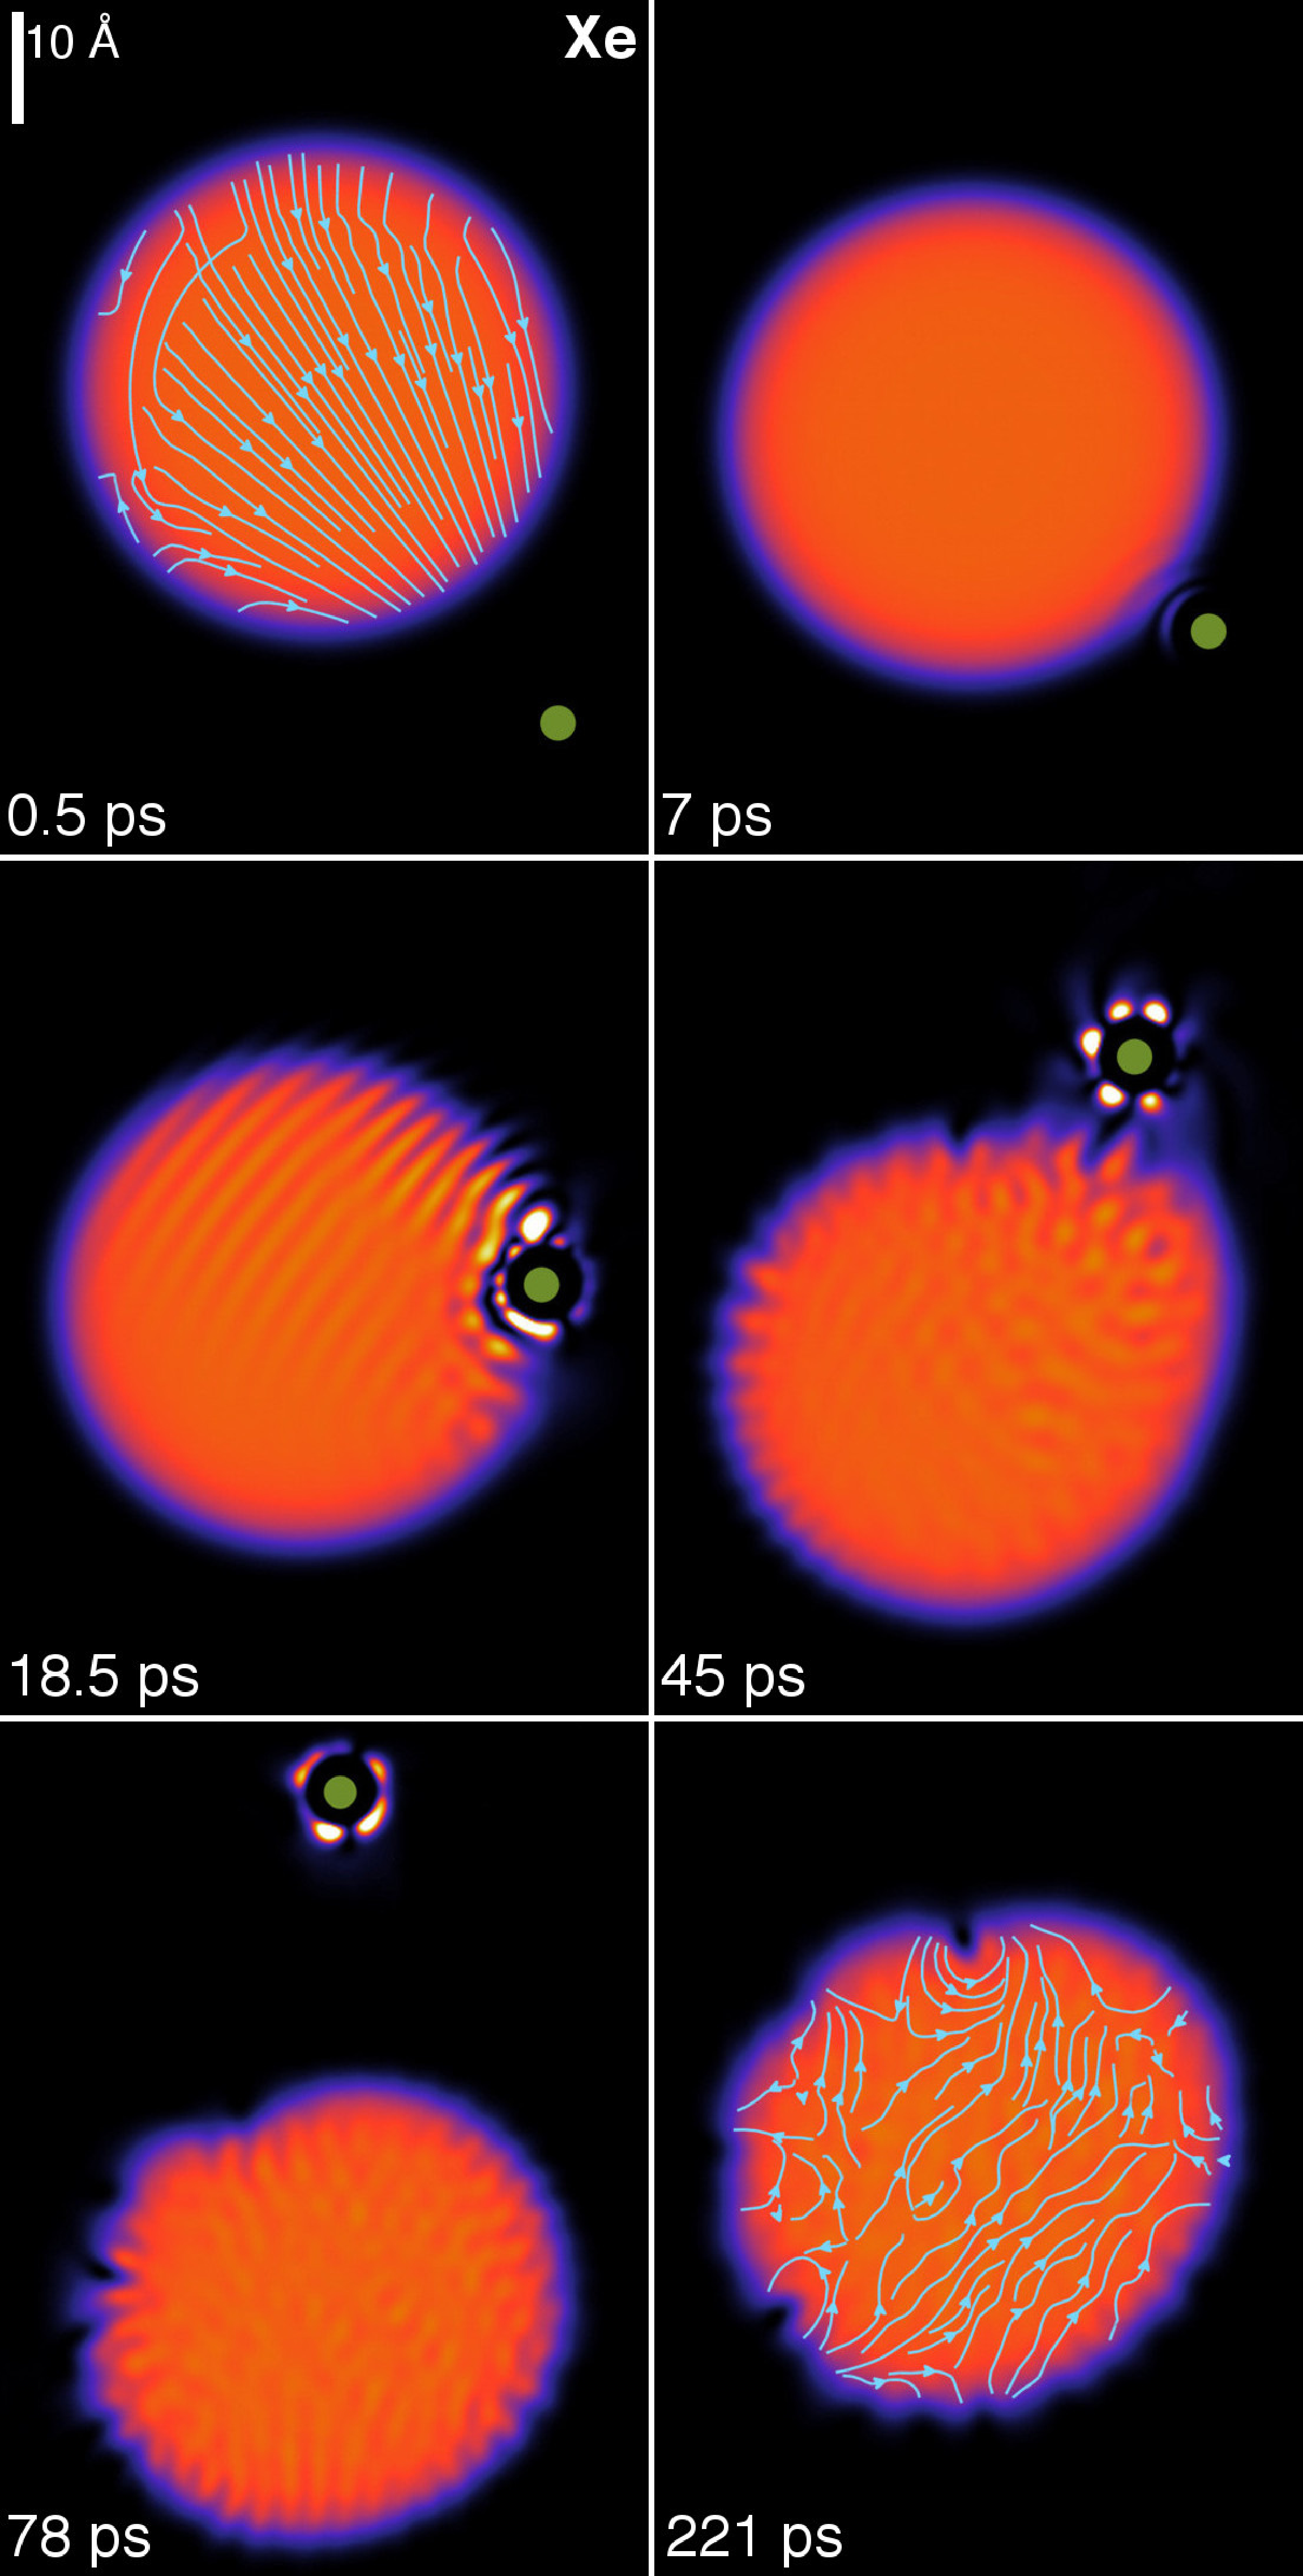
\includegraphics[width=0.60\linewidth,clip]{xehe200-b222-composed}}
\caption{\label{fig6-capture} 
Dynamic evolution of a Xe atom (green dot) approaching the $^4$He$_{1000}$ 
droplet from below at $v_0 = 200$ m/s with impact parameter $b = 22.2$ \AA{}. The corresponding time is indicated in each frame.\citep{ESI}  
}
\end{figure}
%

In peripheral collisions not only energy but also angular momentum 
is deposited into the droplet, which allows  
to visualize the  irrotational flow of the superfluid helium.
In particular,
for Xe at $v_0=$200 m/s and $b$=22.2 \AA{} the initial angular momentum is 917 $\hbar$. 
This collision was followed for some 220 ps and
produced the ejection of 15 He atoms, 5 of them attached to the Xe atom, see Fig. \ref{fig6-capture}. 
After the collision, the Xe+$^4$He$_5$ complex carries away 522 
angular momentum units, while some 95 units are deposited in the droplet as vortex loops and
capillary waves,\citep{Whi98} see bottom right panel of Figs. \ref{fig5-capture} and \ref{fig6-capture}. 
The remaining angular momentum is taken away by the ejected helium atoms.

\subsection{Helium droplets hosting vortex lines}

To determine the structure of a droplet hosting a singly-quantized linear vortex 
we have started the imaginary time iteration from a helium  
density in which the vortex is ``imprinted''. For this purpose, a vortex line
along the $z$  can be described by the effective wave function 
%
\begin{equation}
\Psi_0(\mathbf{r}) =  \rho_0^{1/2}(r) \, e^{\imath  \, {\cal S}(\mathbf{r})} = \rho_0^{1/2}(\mathbf{r}) \, \frac{(x + \imath y)}{\sqrt{x^2 + y^2}} 
\label{eq11}
\end{equation}
%
where $\rho_0(\mathbf{r})$ is the density of 
either the pure or  the impurity-doped droplet without vortex.  
Vortex lines along other directions passing through a chosen point 
can be imprinted as well.\citep{Pi07}
%;  more involved imprinted configurations can be found {\it e.g.} in ref. \citep{Pi07}. 
 
In the case represented by Eq. (\ref{eq11}), if the impurity is within the vortex
core along a symmetry axis of the impurity-droplet complex,
the effective wave function $\Psi_0({\mathbf r})$ -- before and after relaxation -- is an eigenvector of the  angular 
momentum operator  $\hat{L}_z = -\imath \; \hbar \partial/\partial \theta$. 
The angular momentum of the droplet is then
 %
\begin{equation}
\langle \hat{L}_z \rangle = \langle \Psi_0(\mathbf{r}) | \hat{L}_z  | \Psi_0(\mathbf{r}) \rangle = N \; \hbar
\label{eq12}
\end{equation}
%

%As far as the energetics of the impurity-droplet-vortex complex is concerned, 
Different energy balances involving pure and doped droplets 
hosting vortices are defined:\citep{Pi07,Anc15,Dal00}
%
\begin{itemize}

\item
Solvation energy of the impurity:

$ S_X = E(X@^4{\rm He}_N) - E(^4{\rm He}_N)$

\item
Vortex  energy:

$E_V= E(V@^4{\rm He}_N) - E(^4{\rm He}_N)$

\item
Binding energy of the impurity to the vortex: 

$B_X = S_X - \{E[(X+V)@^4{\rm He}_N] - E(V@^4{\rm He}_N)\}$

\end{itemize}
%
Using the functional of ref. \citep{Anc05a} and the He-rare gas pair potentials of ref. \citep{Tan86}, solvation energies
of  -316.3 K and -215.7 K have been  found for Xe and Ar atoms, respectively. Thus, for the same incident kinetic
energy, about 100 K of additional energy have to be dissipated in the case of Xe in order to get the same kinematic conditions than for Ar.

The  binding energy of the impurity to the vortex
is the result of a delicate balance between terms which are
individually much larger than
their difference. It can thus be affected by relatively 
large inaccuracies.
Within DFT, it has been found that the Xe atom
 is barely bound to the vortex line, with $B_{Xe}\sim 3-5$ K.\citep{Dal00,Anc14}

%The kinetic energy of the superfluid flow in the volume excluded by the
%impurity intuitively corresponds to $B_X$. For this reason, $B_X$ is 
%also called  ``substitution energy''.\citep{Don91}
%Using a sharp helium density model for the impurity 
%bubble and the vortex line, it can be shown that\citep{Don91}
%
%\begin{eqnarray}
%&&B_X = 2 \pi \frac{\hbar^2}{m_4} \rho_0  \,R_X \times 
%\\
%\nonumber
%&&
%\left\{\left(1 +  \frac{a^2}{R_X^2}\right)^{1/2} 
%\,ln \left[\frac{R_X}{a} + \sqrt{\left(\frac{R_X}{a}\right)^2+1}\right] - 1 \right\} \; ,
%\label{eq13}
%\end{eqnarray}
%
%where $a$ is the radius of the vortex core and $R_X$ is the radius of the atomic bubble.
%Taking $\rho_0= 0.0218$ \AA$^{-3}${}, $a=1$ \AA{} and $R_X=3.5$ \AA{},  
%which corresponds to the value where the Xe-He pair potential becomes repulsive,
%one obtains $B_{Xe}= 6.1$ K. In the case of Ar, $R_X$=3.1 \AA{} and $B_{Ar}$=4.8 K.

A critical angular velocity $\omega_c$ exists above which nucleation of
vortices with quantized velocity circulation in units of $h/m_4$ occurs.
The critical angular velocity for nucleating a vortex line  along a diameter
in a droplet made of $N$ helium atoms is
%
\begin{equation}
\omega_c  = \frac{1}{\hbar}\,\frac{E_V}{N} 
\label{eq14}
\end{equation}
%
This expression is obtained by computing the energy that 
minimizes $\langle H -\omega L_z\rangle$ ({\it i.e.} corresponding 
to the equilibrium configuration in the corotating frame) with and without 
a vortex line.
%\citep{Dal96} 
Using the values appropriate for a $^4$He$_{1000}$ 
droplet we obtain $\omega_c =  0.127$ K/$\hbar$ = 0.0167\,  ps$^{-1}$.

%The velocity field corresponding to axially symmetric configurations with one vortex along the $z$-axis is
%
%$$ \mathbf{v}(\mathbf{r}) = \frac{\hbar}{m_4} \frac{1}{r} \hat{\theta}$$
%
%where $r$ is the distance to the $z$-axis and 
%$\hat{\theta}$ the unit vector in 
%the increasing $\theta$ direction (counterclockwise);
%the circulation lines on the $x-y$ plane  are circumferences.\citep{Don91} 
%It is worth mentioning that the above velocity field 
%is irrotational, but this is not the only possibility. 
%Indeed, below $\omega_c$ the superfluid droplet may store
%some angular momentum smaller than $\hbar N$ without 
%hosting any vortex; the only constraint is that 
%the velocity field of the superfluid must be irrotational. 
%We will come back to this point later on.

When the angular velocity is increased 
above $\omega_c$, larger amounts of angular momentum may be stored
into the superfluid by increasing the number of 
nucleated vortices. The higher the angular velocity,  
the more packed the vortex array is
around the rotation axis.  
These vortices arrange themselves into ordered structures  
whose existence in bulk superfluid $^4$He was established long  ago.\citep{Vin61,Wil74}

To generate vortex arrays we have worked in the  
fixed-droplet frame of reference (corotating frame at  
angular velocity $\omega$), {\it i.e.} we look for solutions of the following EL equation: 
%
\begin{equation}
\{{\cal H}[\rho] \,-\omega \,\hat{L}_z\} \,\Psi(\mathbf{r})  =  \,\mu_4 \,
\Psi(\mathbf{r}) \;,
\label{eq15}
\end{equation}
%
In this case, $\Psi(\mathbf{r})$ no longer is  
an eigenvector of the angular momentum.
To determine $\Psi(\mathbf{r})$ describing a 
configuration where $n_v$ vortex lines are present we have followed 
again the imprinting strategy, starting the imaginary-time evolution of  
Eq. (\ref{eq15}) with the helium effective wave function
%
\begin{equation}
\Psi_0(\mathbf{r})=\rho_0^{1/2}(\mathbf{r})\, \prod _{j=1}^{n_v} \left[ {(x-x_j)+\imath (y-y_j) \over \sqrt{(x-x_j)^2+(y-y_j)^2}}  \right] 
\label{eq16}
\end{equation}
%
where  $\rho_0(\mathbf{r})$ is the density of the vortex-free 
droplet and $(x_j, y_j)$ is the initial position of the $j$-vortex linear  core with
respect to the $z$-axis of the droplet (note that in refs. \citep{Anc14,Anc15}  
$\Psi_0(\mathbf{r})$ was incorrectly written).
We underline the fact that during the functional minimization 
of the total energy, the vortex positions and shapes will change
to provide at convergence the lowest energy vortex 
configuration for the given value of the angular velocity $\omega$.  

\begin{figure}[h]
\centerline{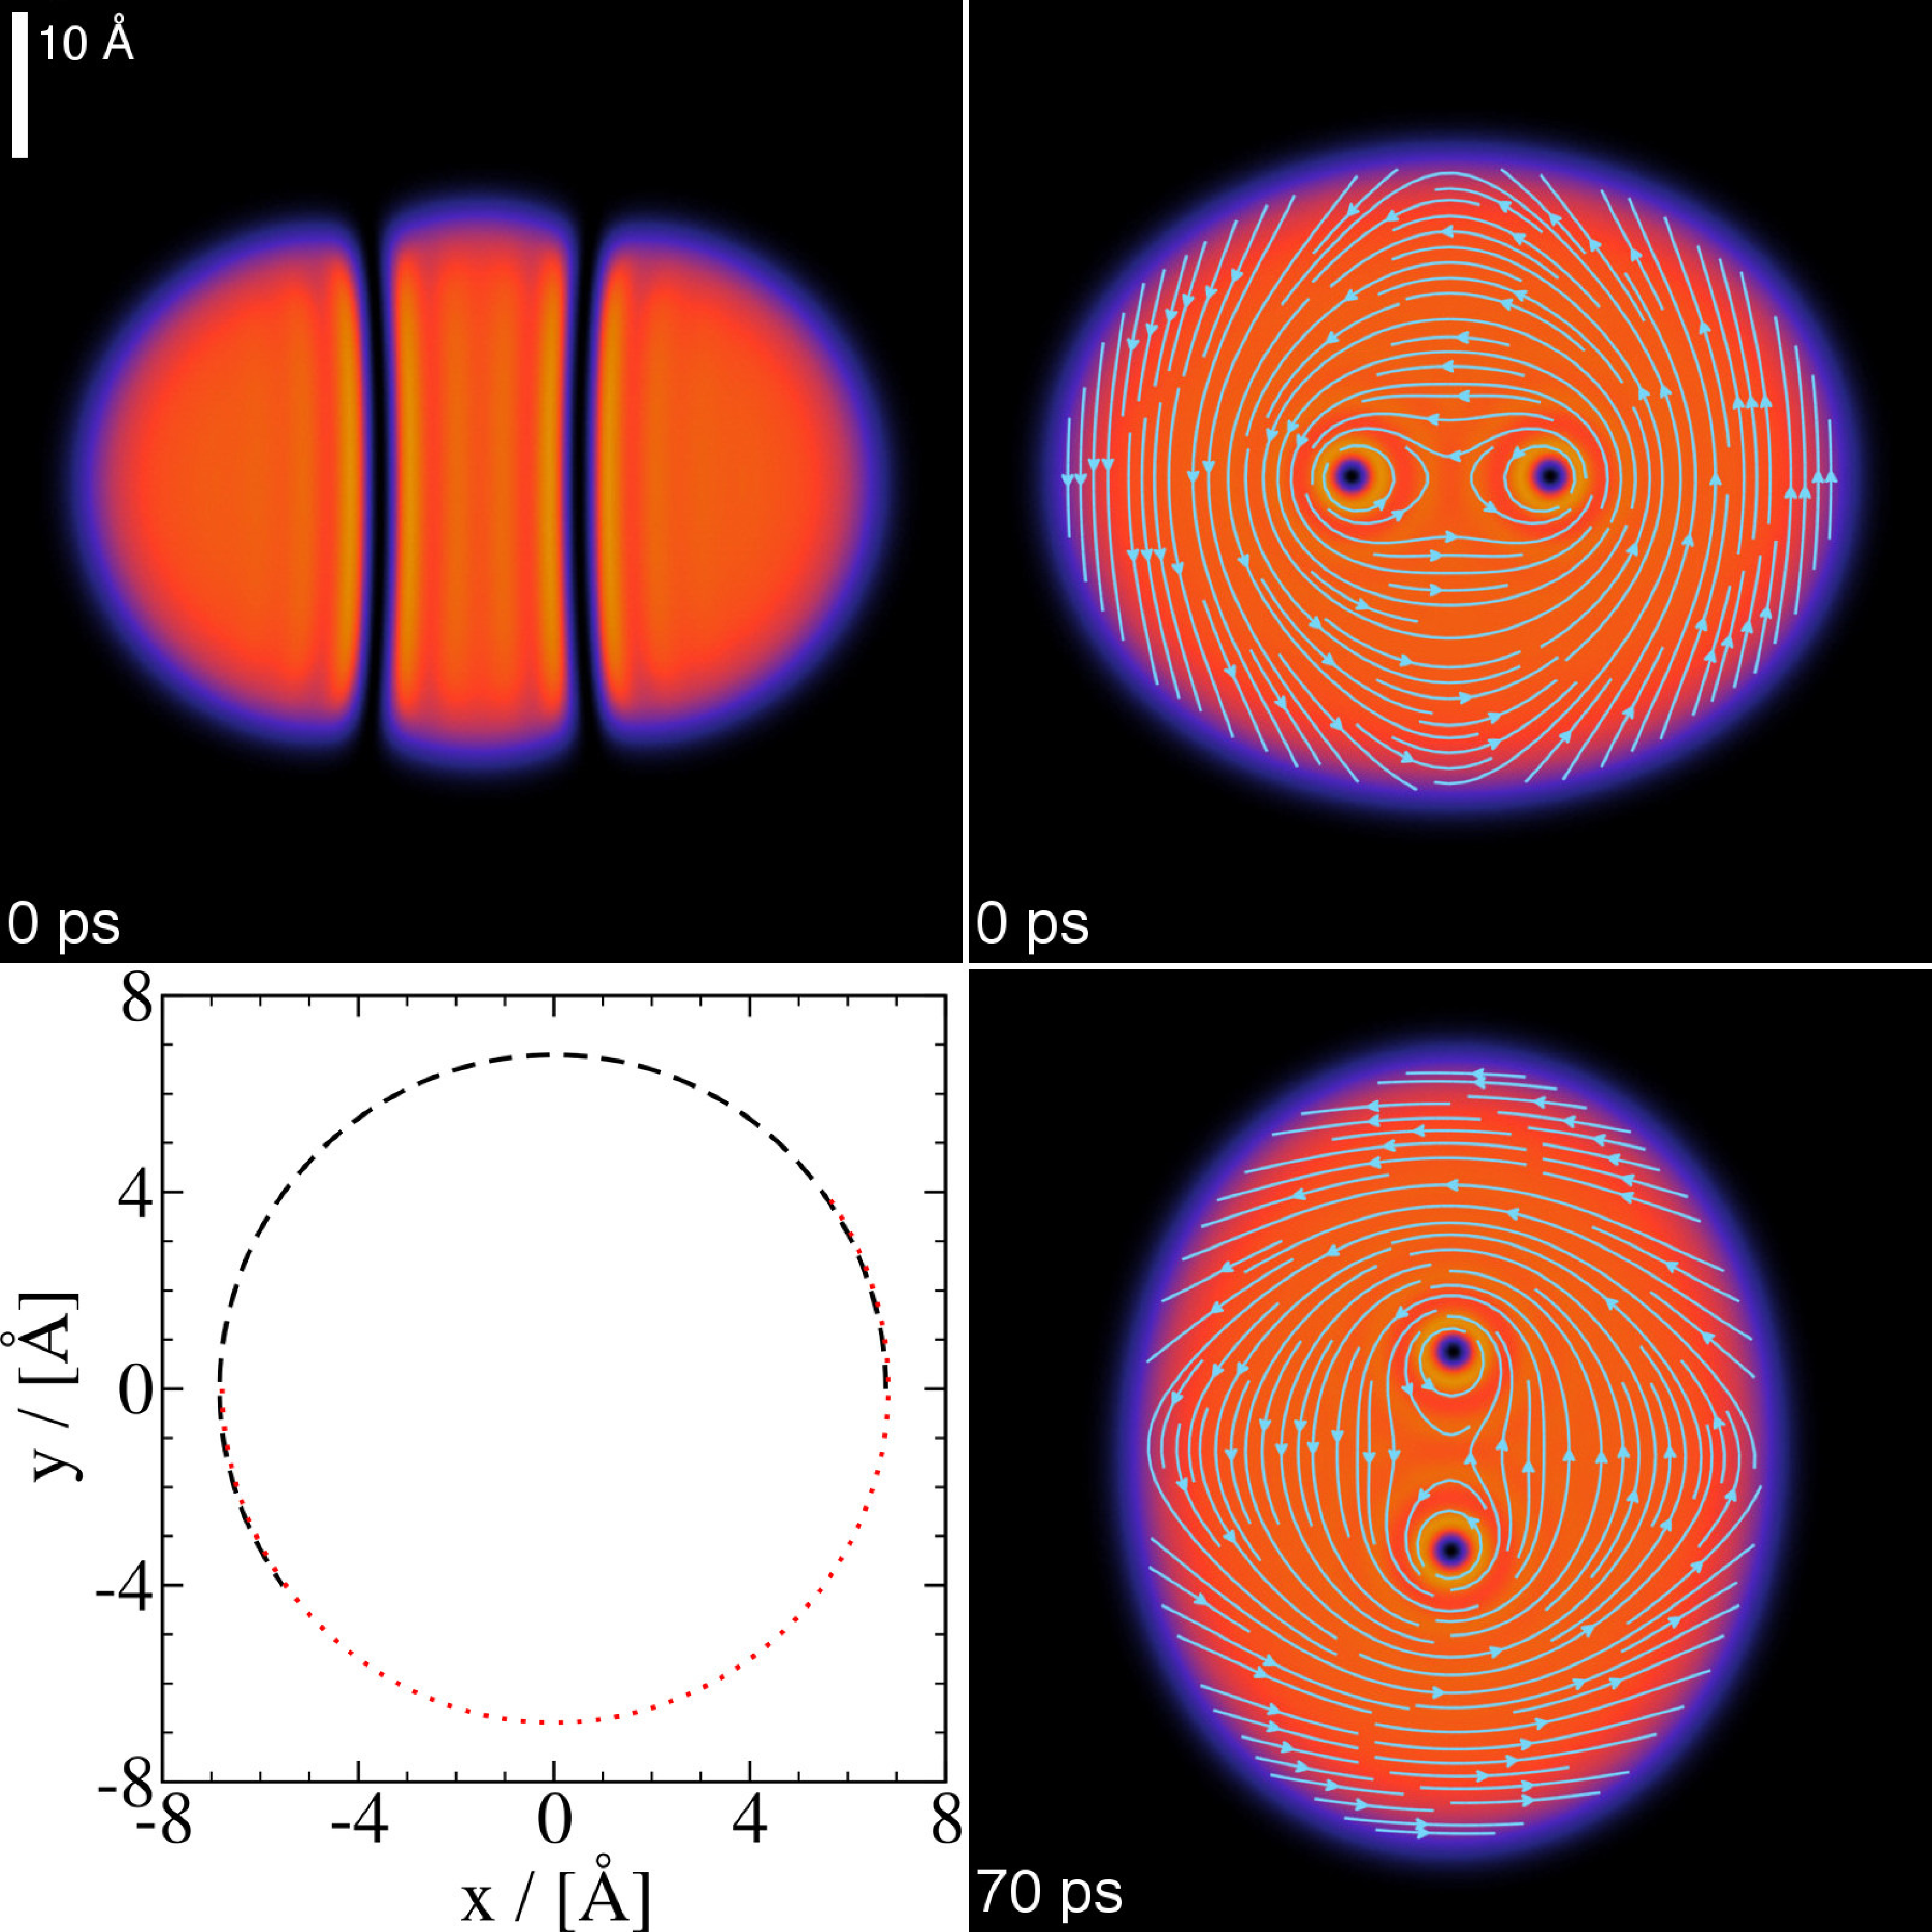
\includegraphics[width=0.8\linewidth,clip]{fig7}}
\caption{\label{fig7-capture}
$^4$He$_{1000}$ droplet at $\omega= 0.0229$ ps$^{-1}$: Top panels, stationary 
two-vortex configuration on the $x-z$ plane (left) and  $x-y$ plane (right)  in the corotating frame.
Bottom left panel, trajectory of the vortex cores 
in the $x-y$ plane of the laboratory frame. 
The dashed line is the trajectory of one of the vortex cores, and the dotted line that of the other. Both trajectories  overlap for a rigid rotation of the cores.
Bottom right panel, helium density in the $x-y$ plane at $t=70$ ps obtained in the laboratory frame starting from the above configuration.\citep{ESI} 
}
\end{figure}

Figure \ref{fig7-capture} shows the two-vortex  
stationary configuration of a $^4$He$_{1000}$ droplet  in the corotating frame 
at angular frequency $\omega$= 0.175 K/\,$\hbar=$ 0.0229 ps$^{-1}$. 
The angular momentum  of this configuration is  $\langle \hat{L}_z \rangle = 1836 \; \hbar$. 
Notice the bending 
of the vortex line so that they meet  
the droplet surface perpendicularly at both ends, and also the 
flattening of the droplet in the $z$ direction
due to centrifugal forces.

At variance with the single vortex line along the symmetry 
axis of the droplet, the two-vortex  configuration is not stationary in the laboratory frame, 
where the density and velocity field change with time. 
To show this, $\Psi(\mathbf{r})$ has been evolved 
in the laboratory  for about 150 ps
taking as initial condition the stationary 
configuration in the corotating frame. 
As expected, the vortex cores appear to rotate in the laboratory frame. 
Within the numerical accuracy, they do so rigidly. This can be seen in 
Fig. \ref{fig7-capture}. Besides, they rotate precisely at 
$\omega$= 0.0229 ps$^{-1}$. This is a  stringent test 
on the accuracy of the dynamics and the consistency of the method.
It can be seen in the ESI$\dag$ 
material how  the two vortex lines turn around each other.

Figure \ref{fig7-capture} shows how a superfluid droplet 
hosting a vortex array ``rotates''. The fact that the vortex 
cores rotate rigidly is not in 
contradiction with the irrotational character 
of the superfluid flow, since they are empty.  The cores carry 
along with them the superfluid whose velocity field  is irrotational,
whereas for a rigid solid or a classical liquid in steady flow 
 one has $\mathbf{v} = \omega \times \mathbf{r}$,  hence $\nabla \times \mathbf{v} = 2\, \omega$. 
The circulation lines in Fig. \ref{fig7-capture} do not correspond 
to a rigid rotation, but to  an irrotational flow in the presence of two vortices. 
The helium density adapts to the vortex cores as they 
rotate and this gives the appearance of a solid 
rotation in the laboratory frame, but it is not. 

It is worth discussing the different  configurations 
that may appear when $\omega < \omega_c$. The lowest energy  
corresponds to the current-free ($CF$) $\langle L_z \rangle =0$ configuration. 
Metastable one-vortex ($1V$) configurations  with 
$\langle L_z \rangle  =N \, \hbar$ also exist in this 
angular frequency range.\citep{Anc14,Anc15} Other irrotational ($IR$) configurations
with $\langle L_z \rangle   < N \, \hbar$ do exist, arising  
from  velocity potentials  such as e.g. 
${\cal S}(\mathbf{r}) = \alpha \,xy$. For an  ellipsoidal droplet with a sharp 
surface, the parameter $\alpha$ is related to the 
angular velocity around the $z$-axis and the deformation 
of the ellipsoid, see the Appendix and refs. \citep{Sei94,Boh75,Rec01}. 

These $IR$ configurations may be generated by using  
the phase ${\cal S}(\mathbf{r}) = \alpha \,xy$ in  
Eq. (\ref{eq11}) and minimizing $\langle H - \omega \hat{L}_z \rangle$. 
At a given value of $\omega < \omega_c$, the energies in the 
corotating frame  are ordered as $E_{CF} < E_{IR} < E_{1V}$.
Fig. \ref{fig8-capture} shows the stationary configuration in the 
corotating frame corresponding to  $\omega= 0.10$ K/\,$\hbar$= 0.0131 ps$^{-1}$.
Although this angular frequency is close to  $\omega_c$,
this configuration is hardly distorted and hosts a negligible amount
of angular momentum: less than $5\times 10^{-2}  \, \hbar$,  compared to the value  of $10^3 \,  \hbar$ at $\omega_c$). The circulation lines 
can be analytically calculated if the density 
profile is approximated by that of an ellipsoid with constant density, see the Appendix. 
 
Figures similar to Fig. \ref{fig8-capture} are shown 
in refs. \citep{Sei94,Boh75} for a rotating  
elliptic vessel  filled with  a fluid whose flow is irrotational.
Whereas in the case of a rigid solid or viscous liquid in steady flow
the entire system rotates as a whole, 
an irrotationally flowing  fluid
in a rotating vessel is just pushed
 by the walls of the
container; the same happens for a Bose-Einstein condensed 
gas in a rotating trap.\citep{Rec01} For an isolated
self-bound $^4$He droplet, 
the apparent ``rotation''  of the 
system in the laboratory arises from deformations of the fluid elements constituting the droplet, but not from their local rotation which is forbidden
by the irrotational condition. The vorticity  $\Omega$  [defined in hydrodynamics as\citep{Guy15}  $\Omega= \nabla \times \mathbf{v}(\mathbf{r})$], 
initially distributed in the helium droplet when it is in the normal phase,  concentrates in the
vortex lines when the droplet becomes superfluid and its velocity field becomes irrotational. 

The above discussion shows how difficult is to set a superfluid droplet in rotation.
Experimentally \citep{Gom14,Jon16,Ber17} 
the situation is different, since  the helium 
droplet is initially in a normal phase state at a temperature above 
the normal-to-superfluid transition temperature 
$T_{\lambda}$ (about 2.17 K in bulk liquid at 1 bar). As a 
consequence, it may store large amounts of  
angular momentum and experience large deformations. 
Copious  evaporation drives the droplet into a 
superfluid state at a temperature below $T_{\lambda}$ and 
the  angular momentum remaining in the droplet is then  stored 
 in vortex arrays that are being nucleated. 
  
\begin{figure}[h]
\centerline{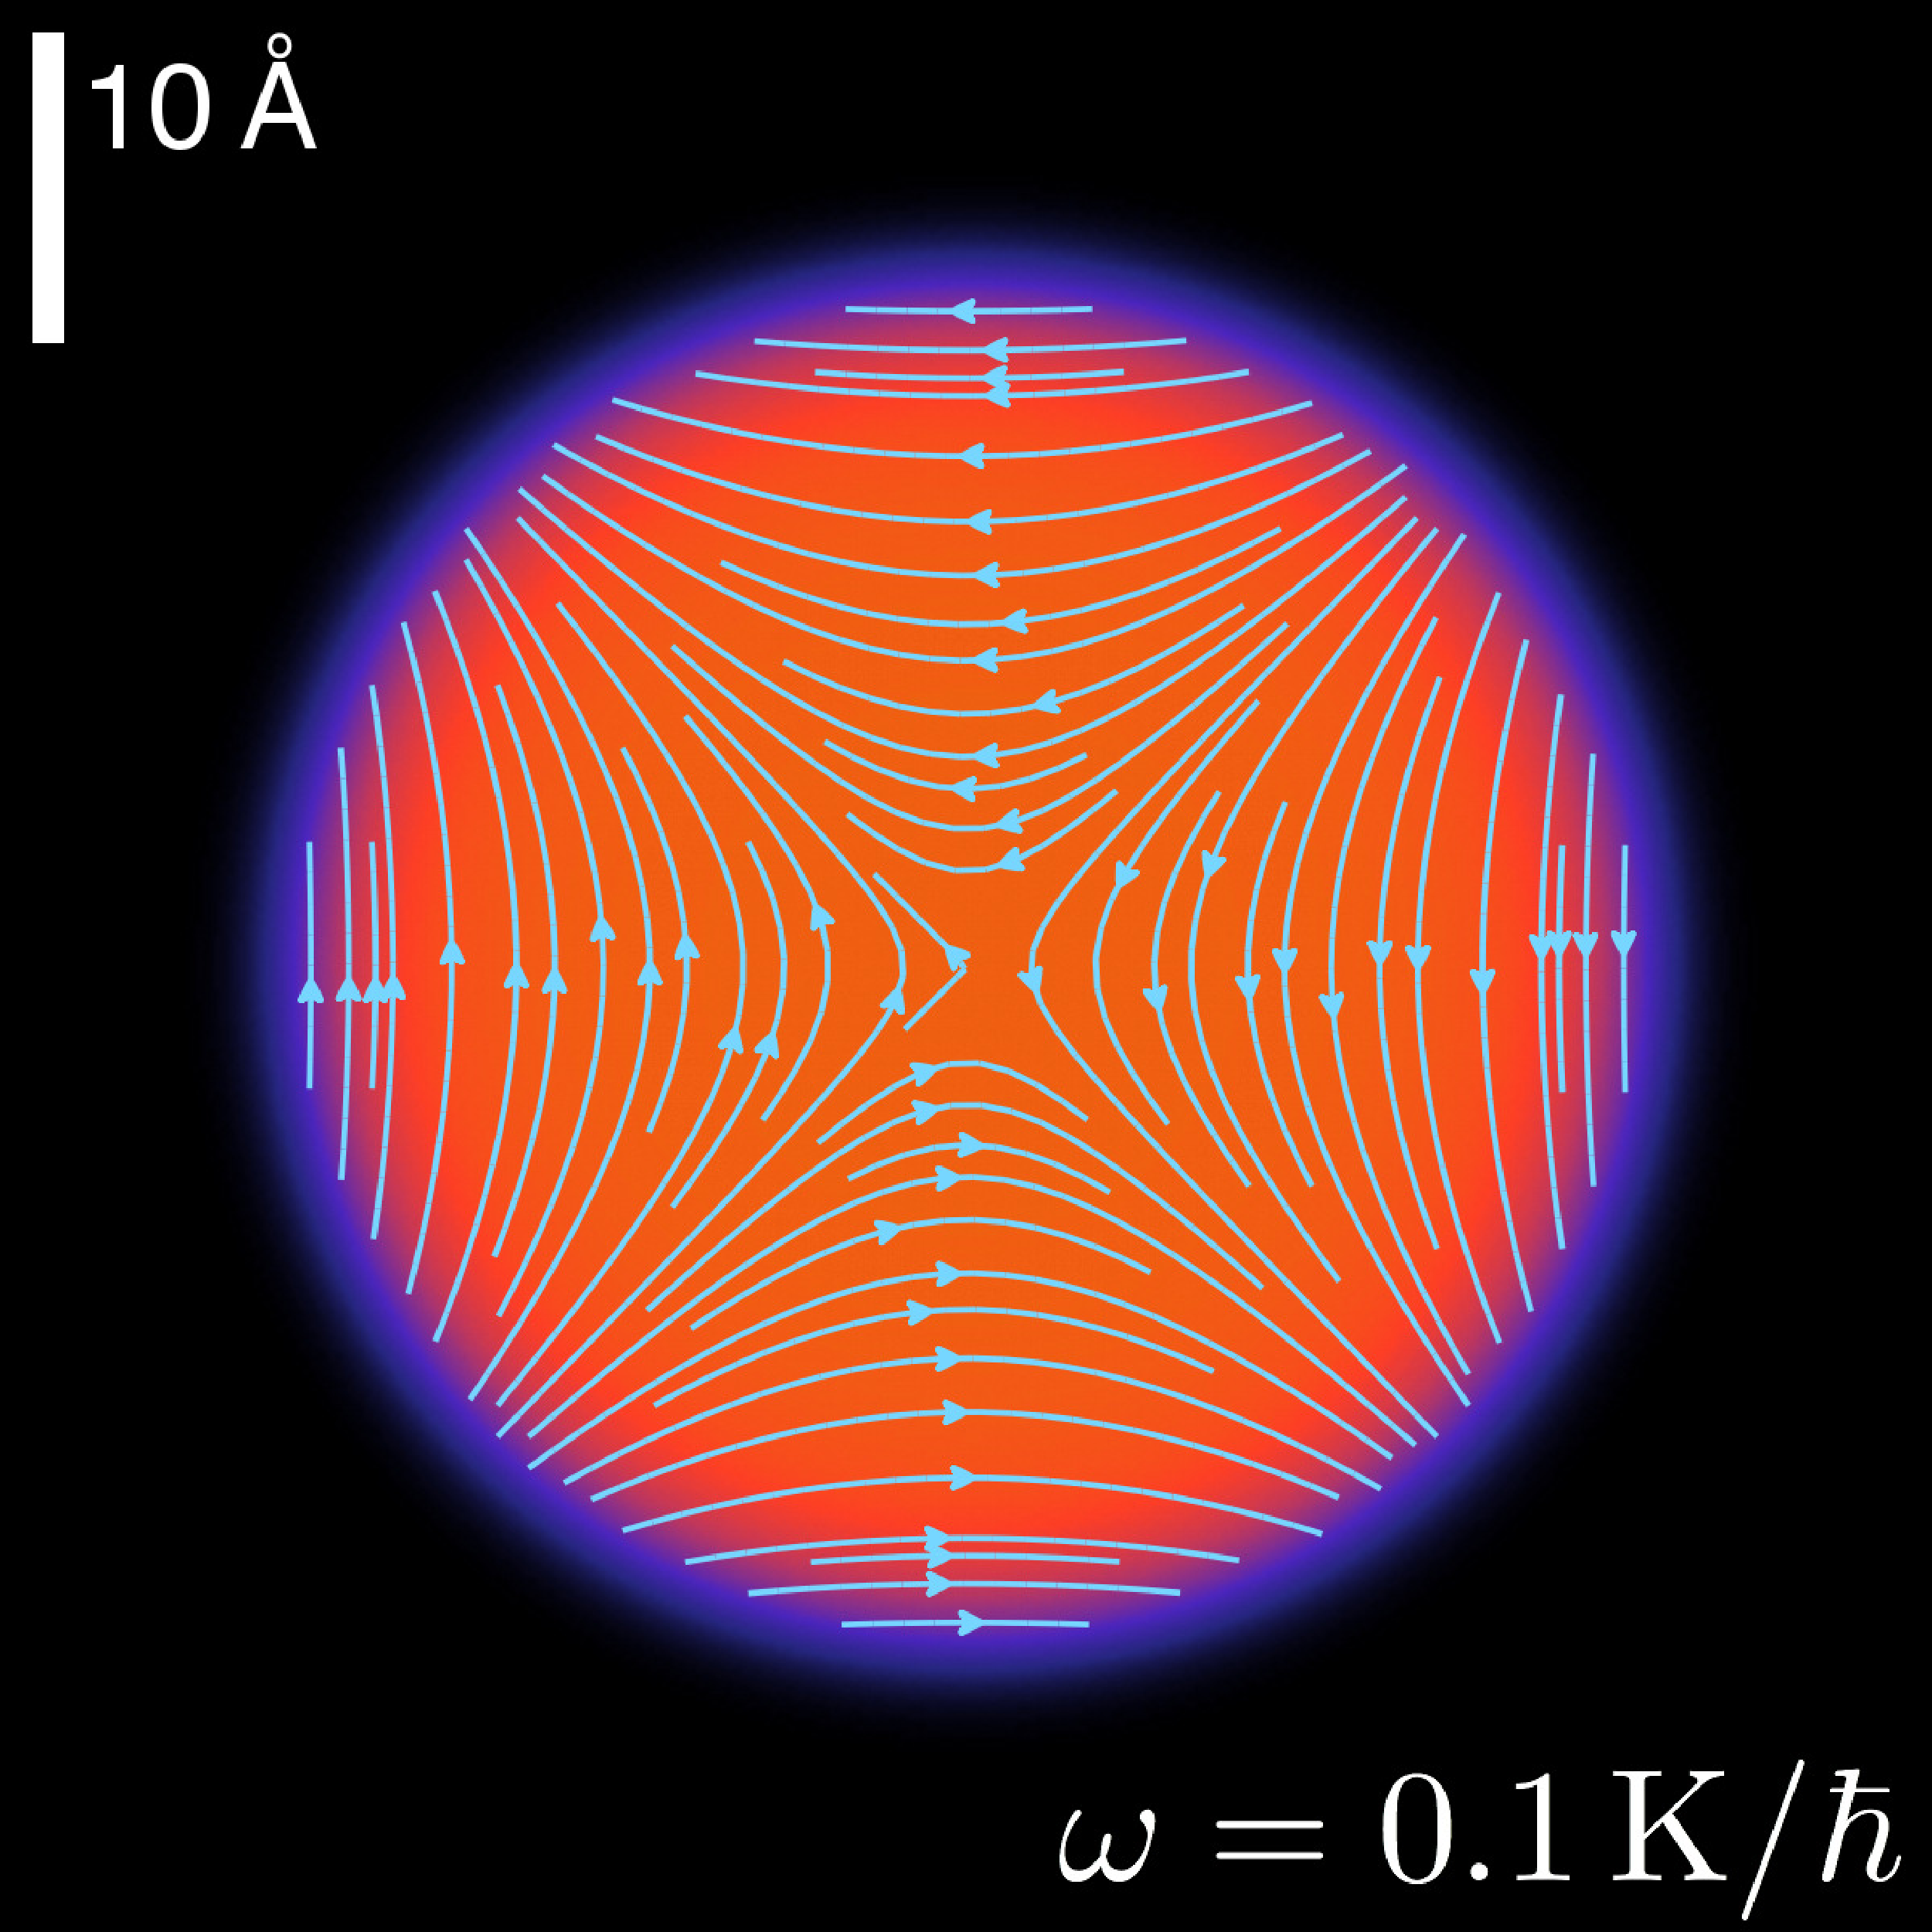
\includegraphics[width=0.7\linewidth,clip]{fig8}}
\caption{\label{fig8-capture}
 Stationary  configuration of the  $^4$He$_{1000}$ droplet at $\omega=$ 0.10 K/$\,\hbar$=0.0131 ps$^{-1}$ in the corotating frame ($x-y$ plane).
}
\end{figure}

%We have also looked at the appearance of vortex-antivortex (vortex dipole) configurations in the droplet. At variance with the two-vortex configuration, the 
%vortex dipole has zero angular momentum and  is stationary
%in the laboratory 
%frame.\citep{Fre10} We have obtained it by the imprinting procedure, giving to the vortex and  antivortex a different sign in the phase
% in Eq. (\ref{eq16}). Since this state has the same angular momentum as the vortex-free ground state of the droplet, we have implemented a Gram-Schmidt 
%orthogonalization procedure to obtain it. Figure \ref{fig9-capture} shows the resulting $^4$He$_{1000}$ droplet vortex dipole configuration. As compared to the two-vortex
%configuration, the droplet is less squeezed and deformed  due to its zero angular momentum.

%\begin{figure}[h]
%\centerline{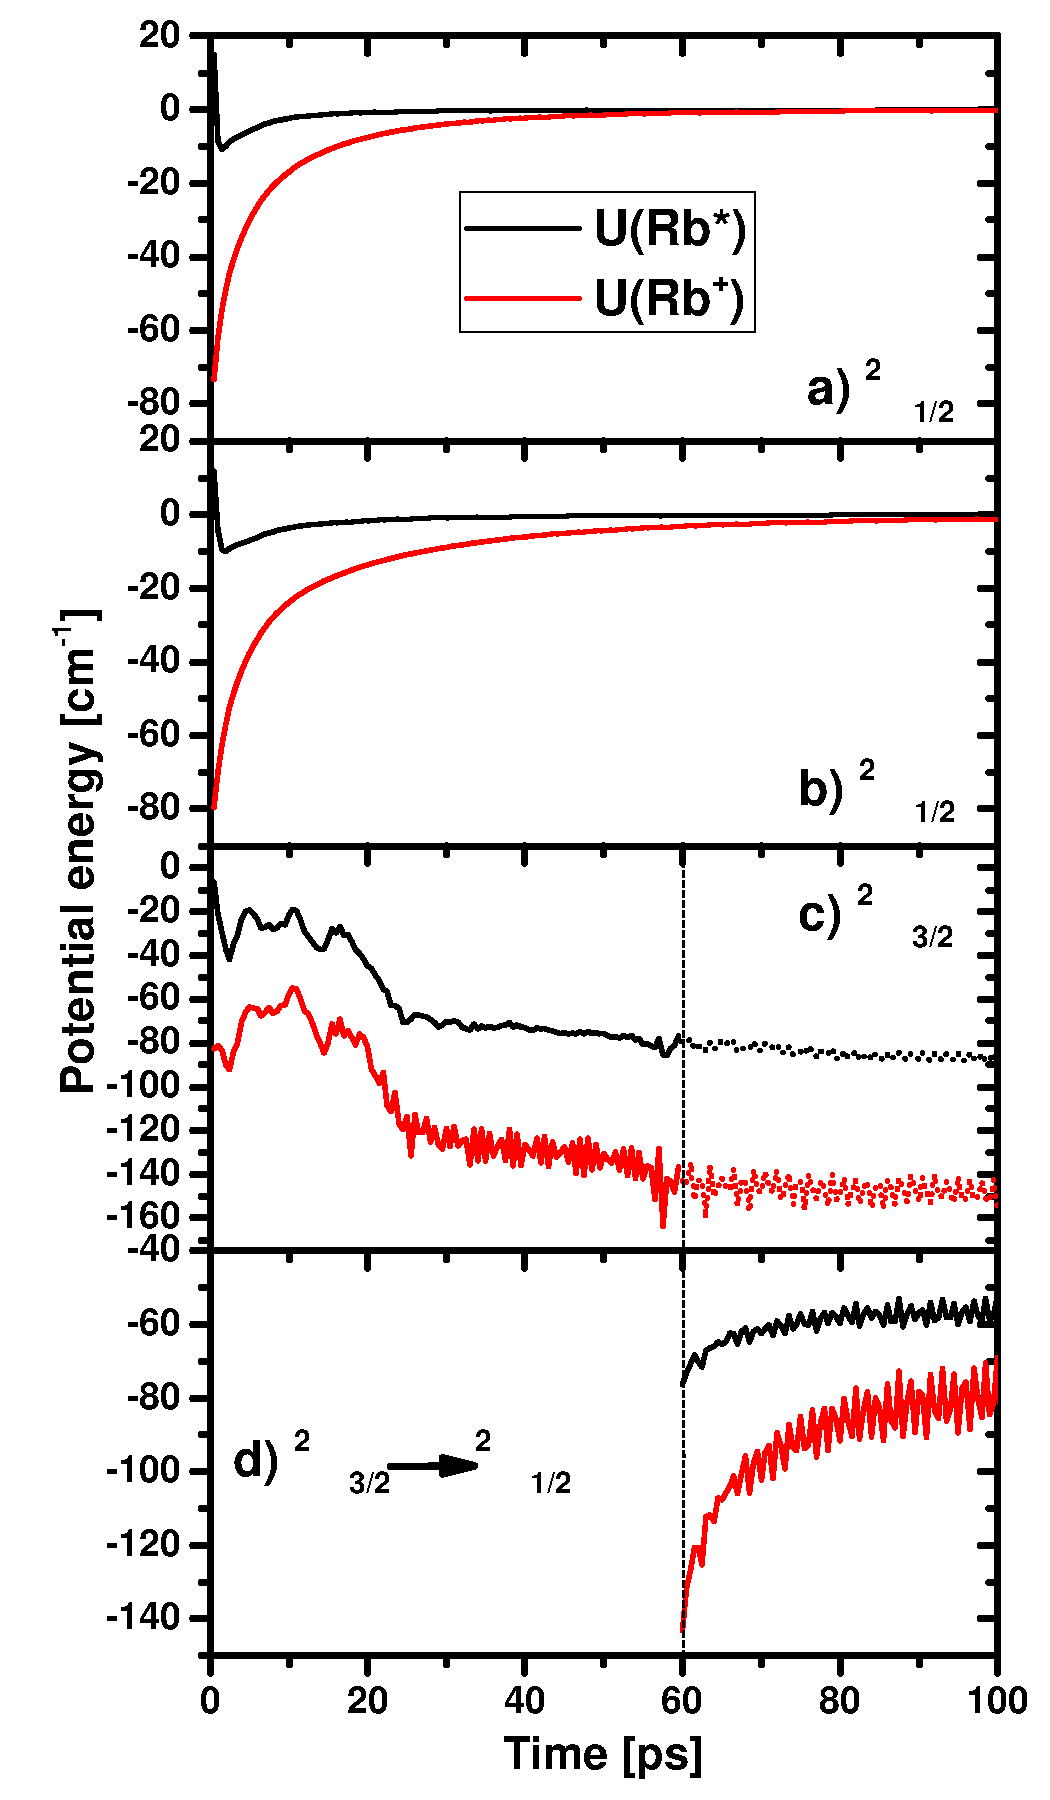
\includegraphics[width=0.9\linewidth,clip]{fig9}}
%\caption{\label{fig9-capture}
%$^4$He$_{1000}$ droplet vortex dipole configuration.  
%The left panel displays the helium density in the $x-z$ plane, and the right panel in the $x-y$ plane. 
%}
%\end{figure}

\subsection{Dynamics of  Xe and Ar capture by vortex lines}

To study the interaction of an atomic impurity with vortices, 
we have imprinted a vortex line in the $^4$He$_{1000}$ droplet 
and prepared the Xe atom in different kinematic conditions. 

%In a first simulation we have initially placed
% the Xe atom  inside the droplet 10 \AA{} away
%from the vortex line,   sending it  head-on towards the vortex at a velocity of 10 m/s.\citep{ESI}
%This velocity  is of the order of the thermal velocity of a Xe atom in a droplet under experimental conditions,
%once the droplet has thermalized after capturing the Xe atoms  ($T \sim$0.4 K).\citep{Toe04}  
%Since the equilibrium position of  the Xe atom is at the center of the droplet, it  moves to this region and remains there during the rest of the simulation.
%In this region of the droplet, the Xe atom is also attracted by the vortex, but it is deflected by the superfluid flow around the vortex line and ends up orbiting around it. 
%Hence it is captured by the vortex without getting into its  core.
%The motion of the  atom
%produces sound waves in the liquid and distortions along of the vortex line (Kelvin modes) that will be shown in detail later.

%The kinematic conditions in the above simulation are similar  to those used for the simulation of inelastic scattering of xenon atoms by quantized vortices in superfluid bulk helium.\citep{Psh16}
% It has been  found in \citep{Psh16} that  a head-on collision leads to the capture of Xe by the vortex line for $v_0=$ 15.4 m/s , but not  for $v_0$=23.7 m/s.
%A detailed  analysis of the Xe capture as a function of the impact parameter has also been  carried out, with the conclusion that when the impact parameter 
% of the Xe atom approaching the vortex line is larger than about 5 \AA{}, Xe is deflected but not captured. In the case of droplets, the final result is very different.
%Upon capture the Xe atom wanders erratically inside the droplet,  as we have seen in the case of vortex-free droplets.
% The surface of the droplet deforms dynamically and acts as
% a ``pinball machine'',  which  eventually brings the Xe atom close enough to the vortex line if it missed it
% in the first attempt and was not previously ejected off the droplet. 
 
 The inelastic scattering of xenon atoms by quantized vortices in superfluid bulk helium has been addressed in ref. \citep{Psh16}.
  It was found that
  a head-on collision leads to the capture of Xe by the vortex line for $v_0=$ 15.4 m/s, but not  for $v_0$=23.7 m/s.
We have carried out  an equivalent  simulation by initially placing
 the Xe atom  inside the droplet 10 \AA{} away
from the vortex line and   sending it  head-on towards the vortex at a velocity of 10 m/s.
This velocity  is of the order of the thermal velocity of a Xe atom in a droplet under experimental conditions,
once the droplet has thermalized after capturing the Xe atom  ($T \sim$0.4 K).\citep{Toe04} 
Since the equilibrium position of  the Xe atom is at the center of the droplet, it  moves to this region and remains there during the rest of the simulation.
In this region of the droplet, the Xe atom is also attracted by the vortex, but it is deflected by the superfluid flow around the vortex line and ends up orbiting around it.
 Hence it is captured by the vortex without getting into its  core.

A detailed  analysis of the Xe capture as a function of the impact parameter has also been  carried out in ref. \citep{Psh16}, with the conclusion that when the impact parameter 
 of the Xe atom approaching the vortex line is larger than about 5 \AA{}, Xe is deflected but not captured.\citep{Psh16}
  In the case of droplets, the final result is very different.
Upon capture, the Xe atom wanders erratically inside the droplet,  as we have seen in the case of vortex-free droplets.
 The surface of the droplet deforms dynamically and acts as
 a ``pinball machine'',  which  eventually brings the Xe atom close enough to the vortex line if it missed it
 in the first attempt or was not previously ejected off the droplet. 

%A more violent event takes place when the Xe atom is initially placed at rest on the droplet surface. This is the smoothest capture process one might think of, as no kinetic energy is 
%initially given to the impurity. The Xe atom is accelerated  towards the center of the droplet due to the attractive He-Xe interaction. 
%We show\citep{ESI}  that, under these kinematic conditions, some He atoms are first drawn towards the  impurity because they are lighter, see also Figs. \ref{fig10-capture} and \ref{fig11-capture}. 
%A similar effect was found in the sinking of Cs$^+$ and Rb$^+$ cations.\citep{Lea14b} 
%Eventually, the impurity with its ``solvation structure'' sinks, acquires some velocity, and is also deflected by the velocity field of the 
%vortex line. 


%A more violent event takes place when. 
The smoothest capture process one might think of corresponds to  the Xe atom being initially placed at rest on the droplet surface, as no kinetic energy is 
given to the impurity. The Xe atom is accelerated  towards the center of the droplet due to the attractive He-Xe interaction. 
We show  that, under these kinematic conditions, some He atoms are first drawn towards the  impurity because they are lighter, see also Figs. \ref{fig10-capture} and \ref{fig11-capture} in ref.~\citep{ESI}. 
%A similar effect was found in the sinking of Cs$^+$ and Rb$^+$ cations.\citep{Lea14b} 
Eventually, the impurity with its ``solvation structure'' sinks, acquires some velocity, and is also deflected by the velocity field of the 
vortex line. 

 We have tried two different initial locations of the Xe atom on the droplet surface.  One is  a point on the equator of the droplet, in a plane perpendicular to the vortex line; 
 the other location is one of the open vortex core ends.  Our aim was to see if a sensible difference in the transit time of Xe across the droplet
could be detected.  The simulations do not show important differences between the time taken by the impurity to reach the center of the droplet. It is about 20 \% larger
when Xe starts from the equator than from the core end.\citep{ESI} It is worth noting that  in the latter case the sliding of the impurity along the core proceeds rather smoothly, and that the impurity
oscillates back and forth much as in the vortex-free case. 

The simulation of Xe ($v_0$=200 m/s) and Ar ($v_0$=360 m/s) atoms head-on colliding with a $^4$He$_{1000}$ droplet perpendicularly to the vortex line has been analyzed and
compared with the result corresponding to a vortex-free droplet. The trajectory of the Xe and Ar atoms in phase space is shown Fig. \ref{fig3-capture}. In both cases the trajectory of the impurity
is limited to the region of the droplet around the vortex line. The impurity orbits around the vortex line because the superfluid flow does so. Since in the DFT approach
no dissipation is included, the signature of the capture of an impurity by a vortex is its close orbiting around the vortex line, as shown in the figure
and especially  in ref. \citep{ESI}. The ESI$\dag$ material shows that whereas Ar is captured during its first transit across the droplet, the Xe atom is only captured in its second transit. We attribute this difference 
to the larger solvation energy of Xe (see Sec. 3.2), which requires more time to be dissipated. It can be seen\citep{ESI} that when Xe detaches from the vortex  in the first
transit,   the  vortex line is reconnected near the atomic solvation structure because no open ends can remain in the bulk of the droplet.
  
%As found in previous simulations,\citep{Lea16,Cop16} 
Figures \ref{fig10-capture} and \ref{fig11-capture} show that
 when the impurity hits the droplet surface a series of surface and volume density waves are launched.
These waves travel  much faster than the impurity itself, 
which has lost a large amount of kinetic energy when it pierced the surface.

The displacement of the  atom in the droplet
produces sound waves in the liquid and distortions along the vortex line (Kelvin modes). 
It is worth seeing that before the bending by the collision with the impurity, the vortex line is twisted (helical Kelvin mode). 
  This  is due to the interference between the  spherical wave front flow
 produced by the hitting of the droplet surface, that travels from bottom to top, 
 and the  flow around the vortex core.
 The spherical wave front  hits first the central portion of the vortex line, whose ends are anchored on the droplet surface. This yields the appearance of the helical distortion
 along the vortex line shown in Fig. \ref{fig12-capture}.
 The twisting  can no longer  be followed after the
 impurity solvation structure reaches the vortex line, bending and dragging it along in the course of its orbiting around it. But it is clearly visible before as shown in Fig. \ref{fig12-capture}, that displays the
 density of the droplet around the vortex line at the indicated collision time. 

\begin{figure}[h]
\centerline{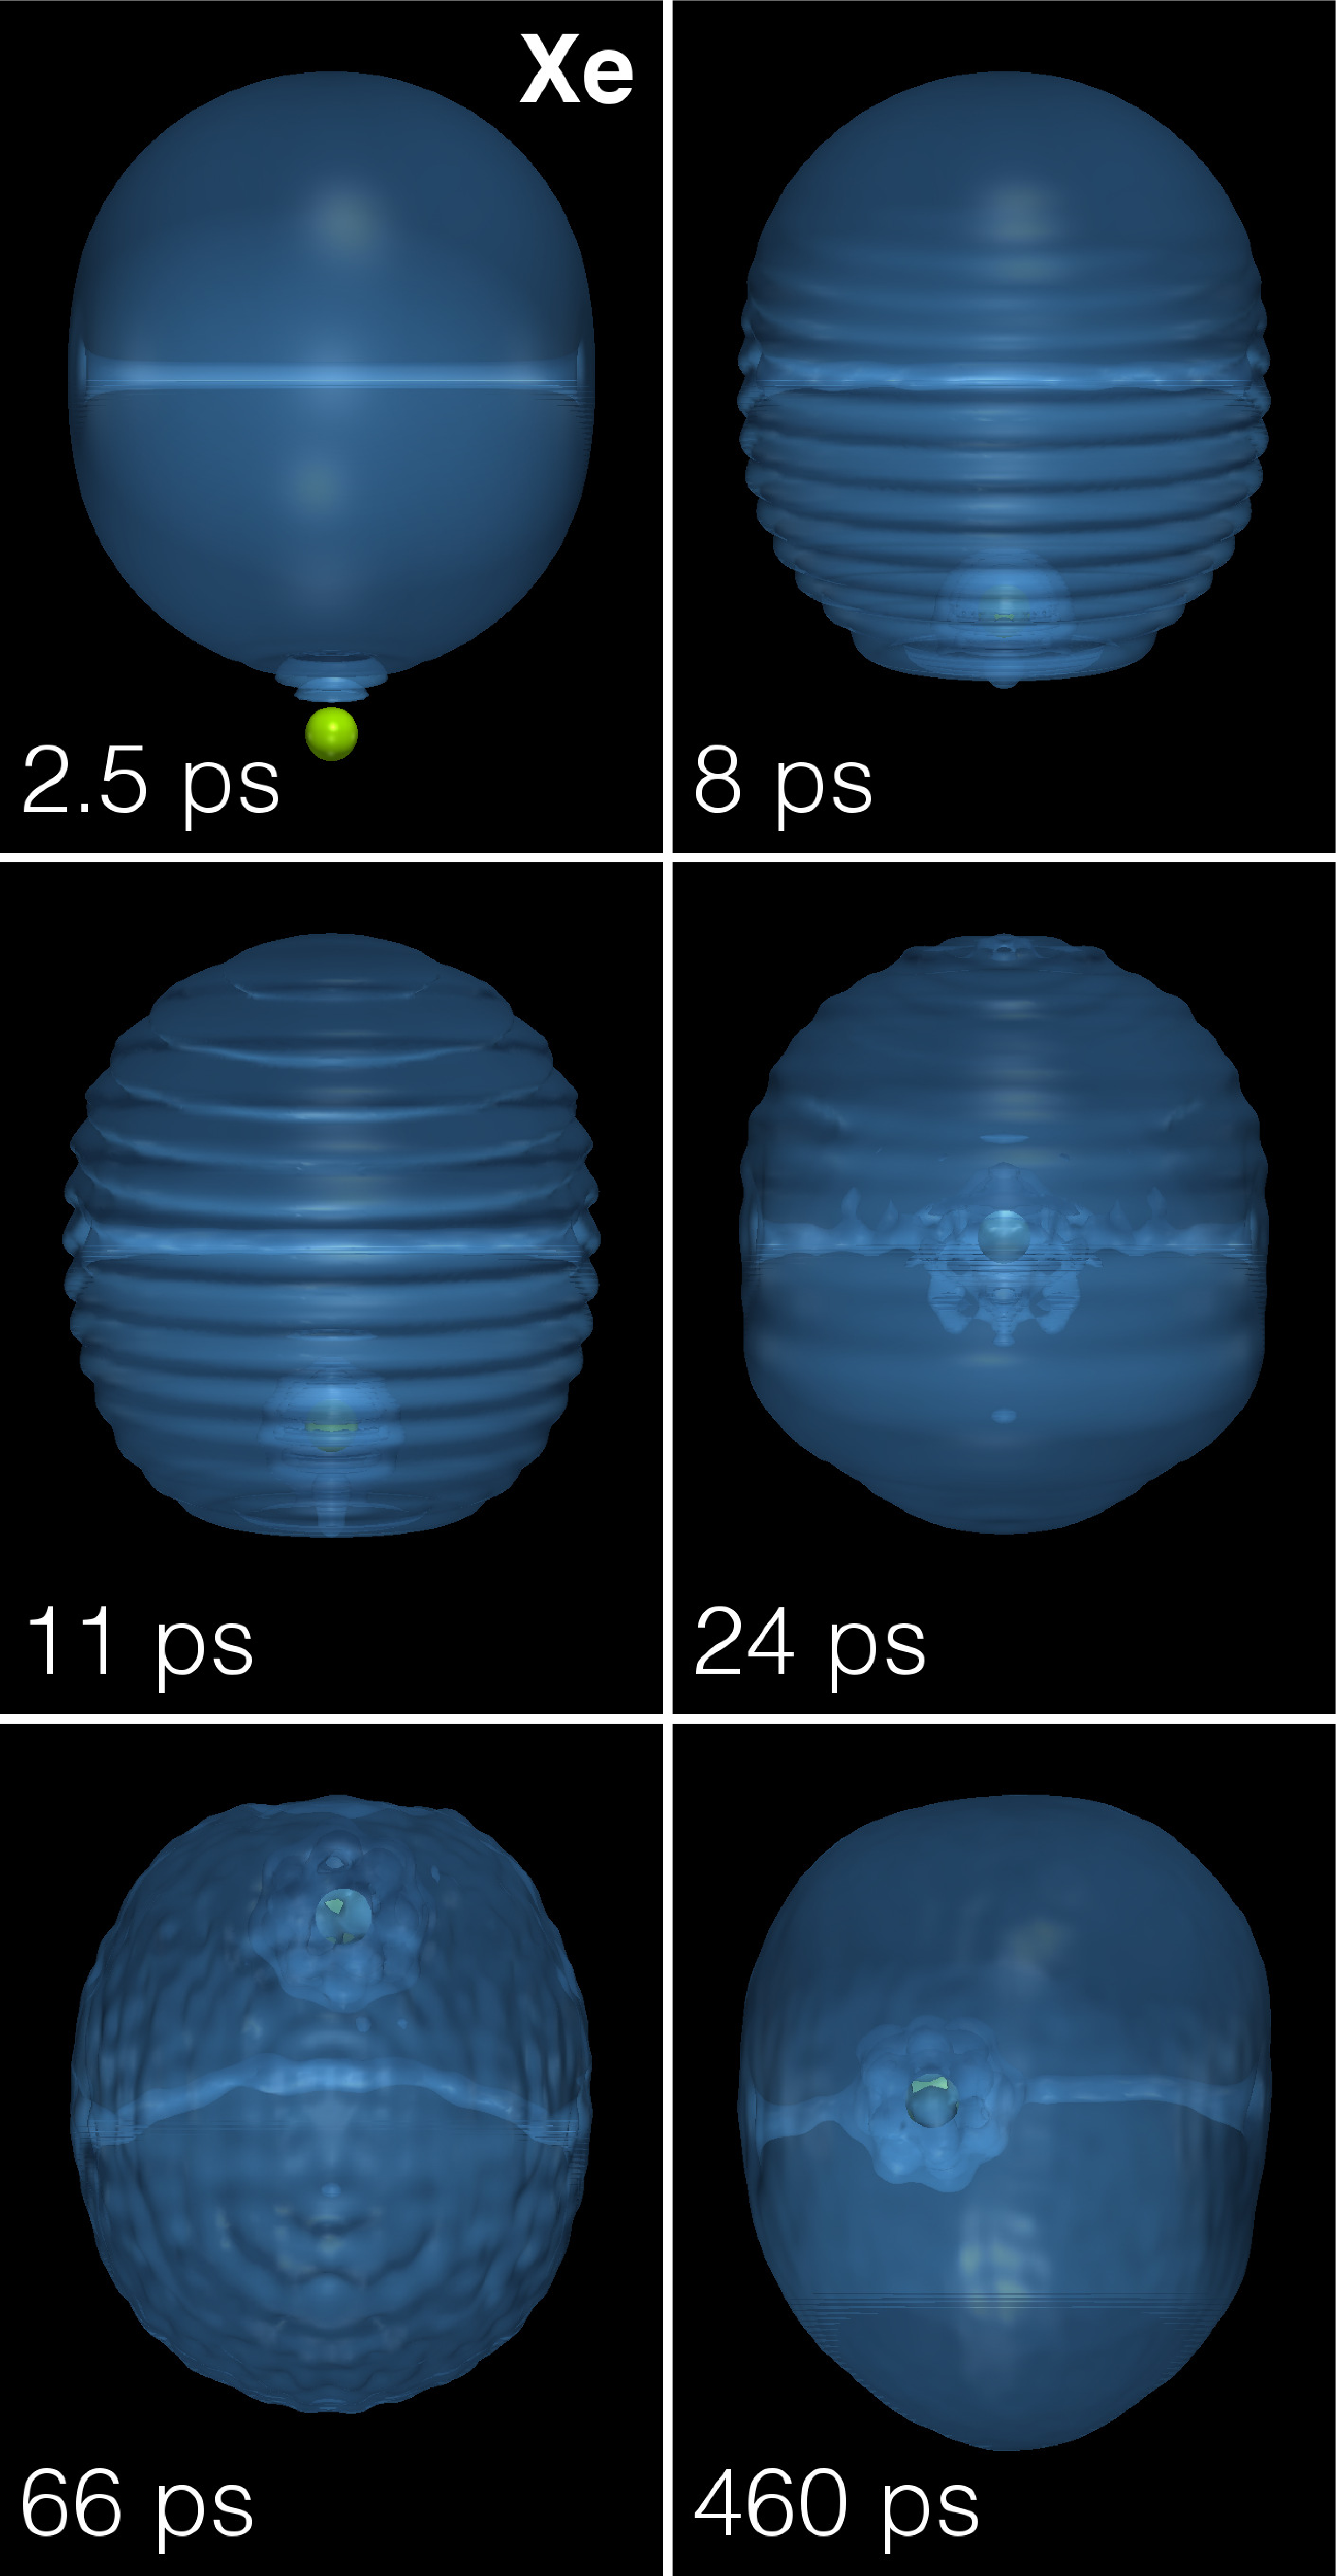
\includegraphics[width=0.60\linewidth,clip]{fig10}}
\caption{\label{fig10-capture}
Dynamic evolution of a Xe atom (green dot) approaching a $^4$He$_{1000}$ 
droplet  hosting a vortex line from below at $v_0 = 200$ m/s. The corresponding time is indicated in each frame.\citep{ESI}  
}
\end{figure}


\begin{figure}[h]
\centerline{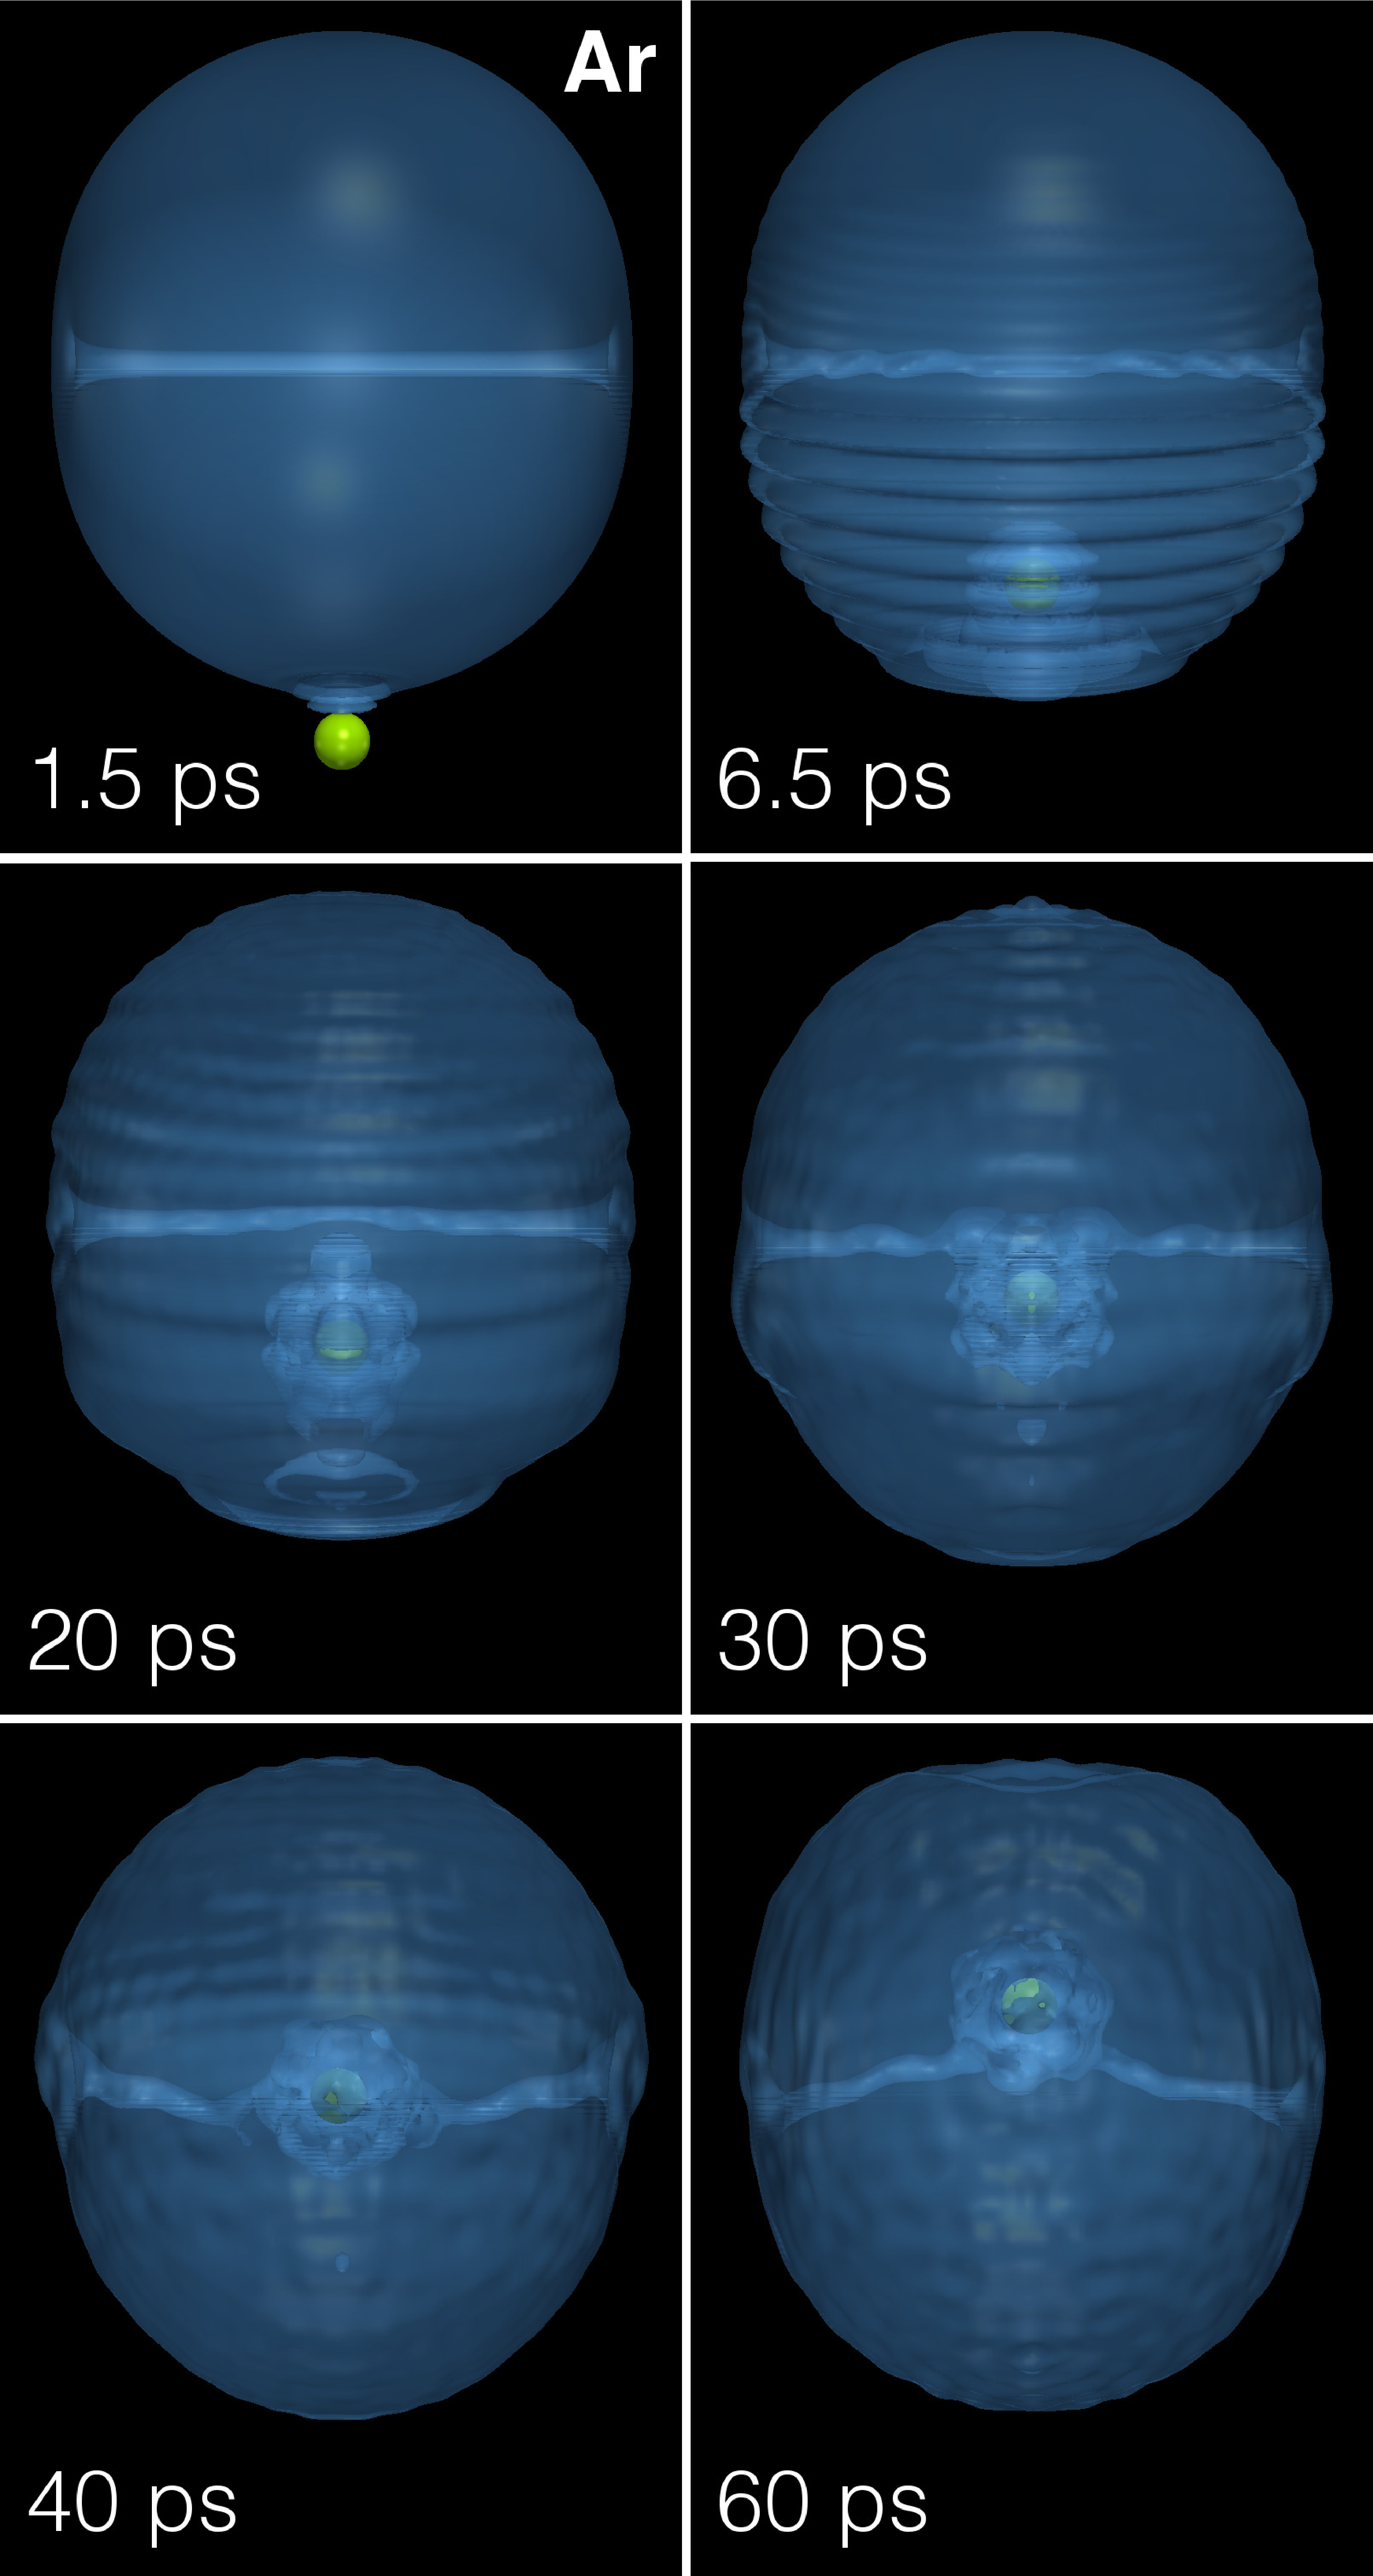
\includegraphics[width=0.60\linewidth,clip]{fig11}}
\caption{\label{fig11-capture} 
Dynamic evolution of an Ar atom (green dot) approaching a $^4$He$_{1000}$ 
droplet  hosting a vortex line from below at $v_0 = 360$ m/s. The corresponding time is indicated in each frame.\citep{ESI}  
}
\end{figure}

 
% Finally, we have simulated the 
%collision of a Xe  atom at 200 m/s against a $^4$He$_{1000}$ droplet hosting a vortex dipole.
%As shown in the  ESI$\dag$ material,\citep{ESI} the Xe atom attaches to either of the vortex cores in the course of the dynamics. After several hundred ps we have 
%found that the impurity eventually gets stuck  to one of the vortices of the dipole and not to both simultaneously. 
%We attribute this to the large superfluid flow in the region between
%them. The situation might change 
%for a configuration made of two vortices with the same sign,
%where superfluid flows tend to cancel out in that region. We have not explored this possibility.   

We have thus shown that   Xe and Ar atoms are readily captured by vortex lines in helium droplets under conditions prevailing in the experiments.\citep{Gom14,Jon16} Simulating the 
capture of a huge number of  impurities or clusters by vortex arrays in  very large droplets is beyond reach at present. However, the results presented in
this subsection are the proof of concept that the limitation is technical and not conceptual.

\begin{figure}[h]
\centerline{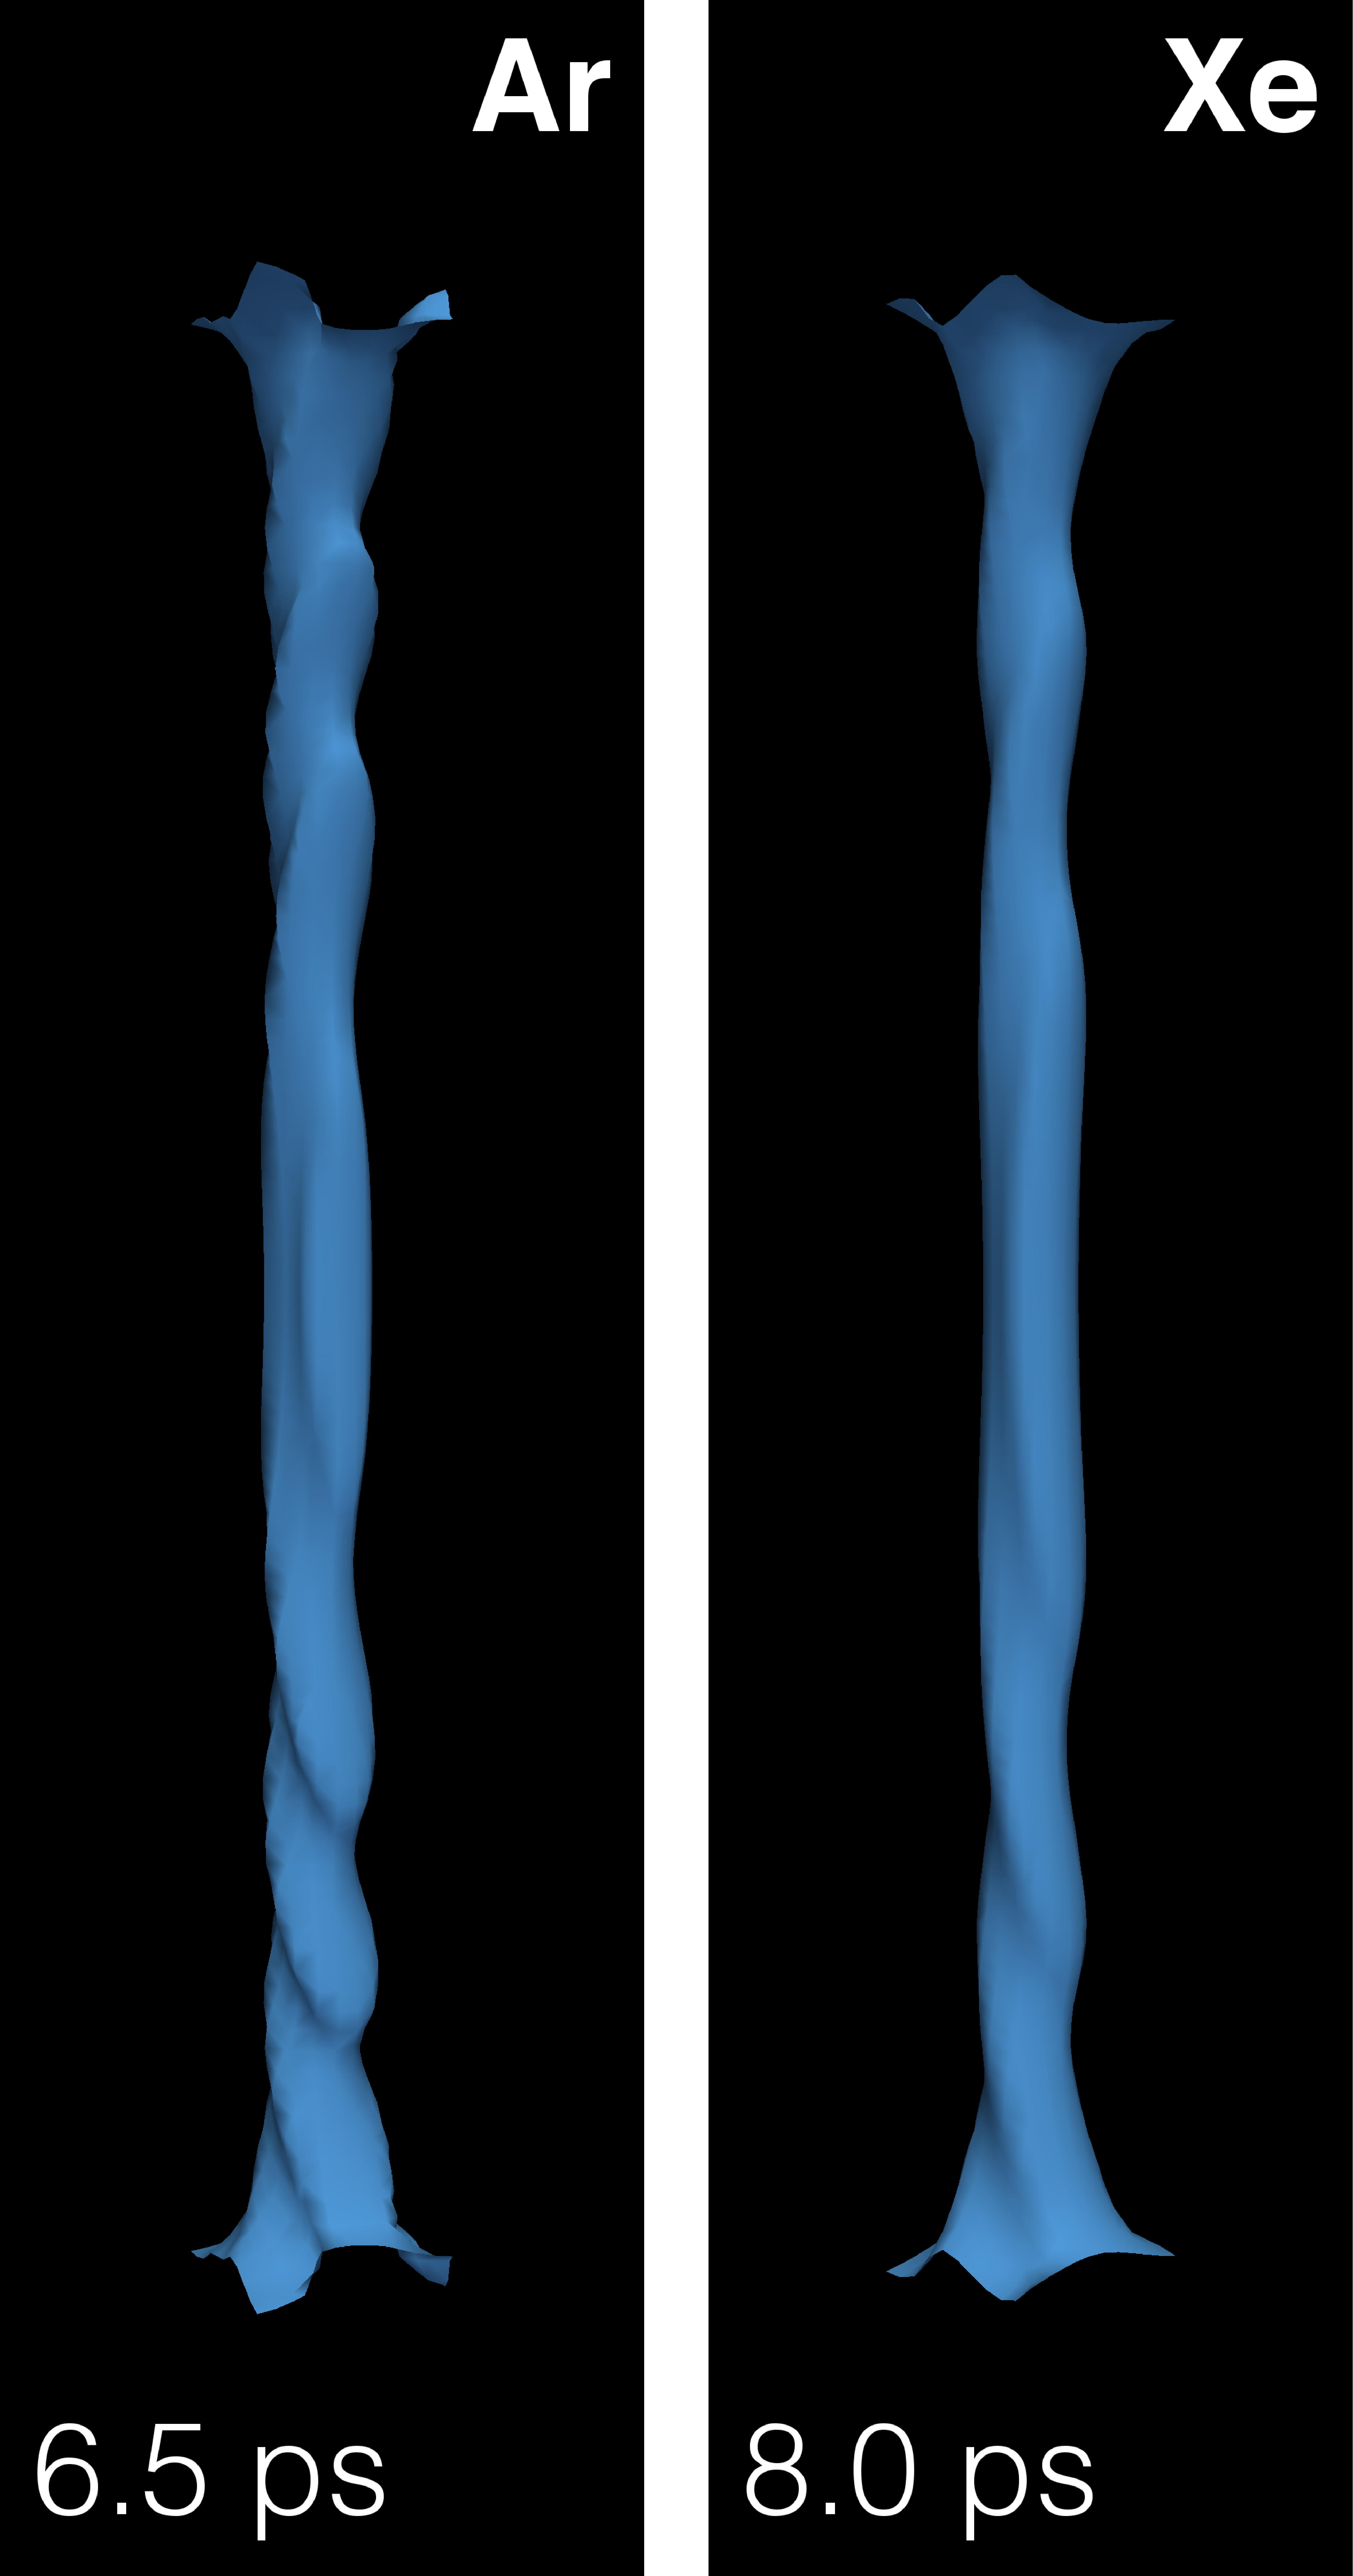
\includegraphics[width=0.60\linewidth,clip]{fig12}}
\caption{\label{fig12-capture} 
Core structure of the vortex line in a $^4$He$_{1000}$ droplet after colliding  with  Xe at $v_0$=200 m/s (right panel, $t= 8$ ps) and Ar at 360 m/s (left panel, $t$=6.5 ps). 
The  full structure of the droplet is shown in Figs. \ref{fig10-capture} and \ref{fig11-capture}.
}
\end{figure}
  
\subsection{Vortex arrays in $^4$He droplets doped with Ar atoms}

The existence of ordered vortex lattices inside $^4$He droplets has been established  by the appearance of Bragg patterns from 
Xe clusters trapped inside the vortex cores  in droplets made of $N= 10^8 - 10^{11}$ atoms
(corresponding to radii from 100 to 1000 nm).\citep{Gom14,Jon16}  We have 
recently studied the stability of vortex 
arrays made of up to $n_v=9$ vortices
inside a $^4$He nanodroplet using the DFT approach.\citep{Anc15}  
It was found that 
the energetically favored structure for $n_v > 6$ is a ring 
of vortices encircling a vortex at the center of the droplet.
Fot $n_v=6$,  the 
configuration with a six-vortex ring is found to have almost 
the same energy as the five-fold ring
plus a vortex at the center. The former structure 
has been experimentally observed,\citep{Gom14,Jon16,Ber17} 
although classical vortex theory 
predicts for it a much higher free energy cost than for the latter.\citep{Cam79}
Similar equilibrium structures have been obtained within DFT for
helium nanocylinders hosting vortex arrays.\citep{Anc14}

In the experiments of ref. \citep{Jon16} the diffraction images 
show that rotating $^4$He nanodroplets of about 200 nm in diameter 
contain a small number of symmetrically arranged quantum 
vortices whose cores are filled with regularly spaced 
Xe clusters. Unexpected large distances 
of the vortices from the droplet center ($\sim 0.7-0.8$ droplet radii) 
are observed and explained as a result of the balance between 
the contribution of the Xe atoms to the total angular momentum of the droplets and 
the solvation potential of the embedded Xe atoms, which opposes the migration of vortices
towards the droplet surface and their annihilation there, as it would
happen instead in the case of undoped vortices for low values of the
droplet rotational frequency.

\begin{figure}[!]
\centerline{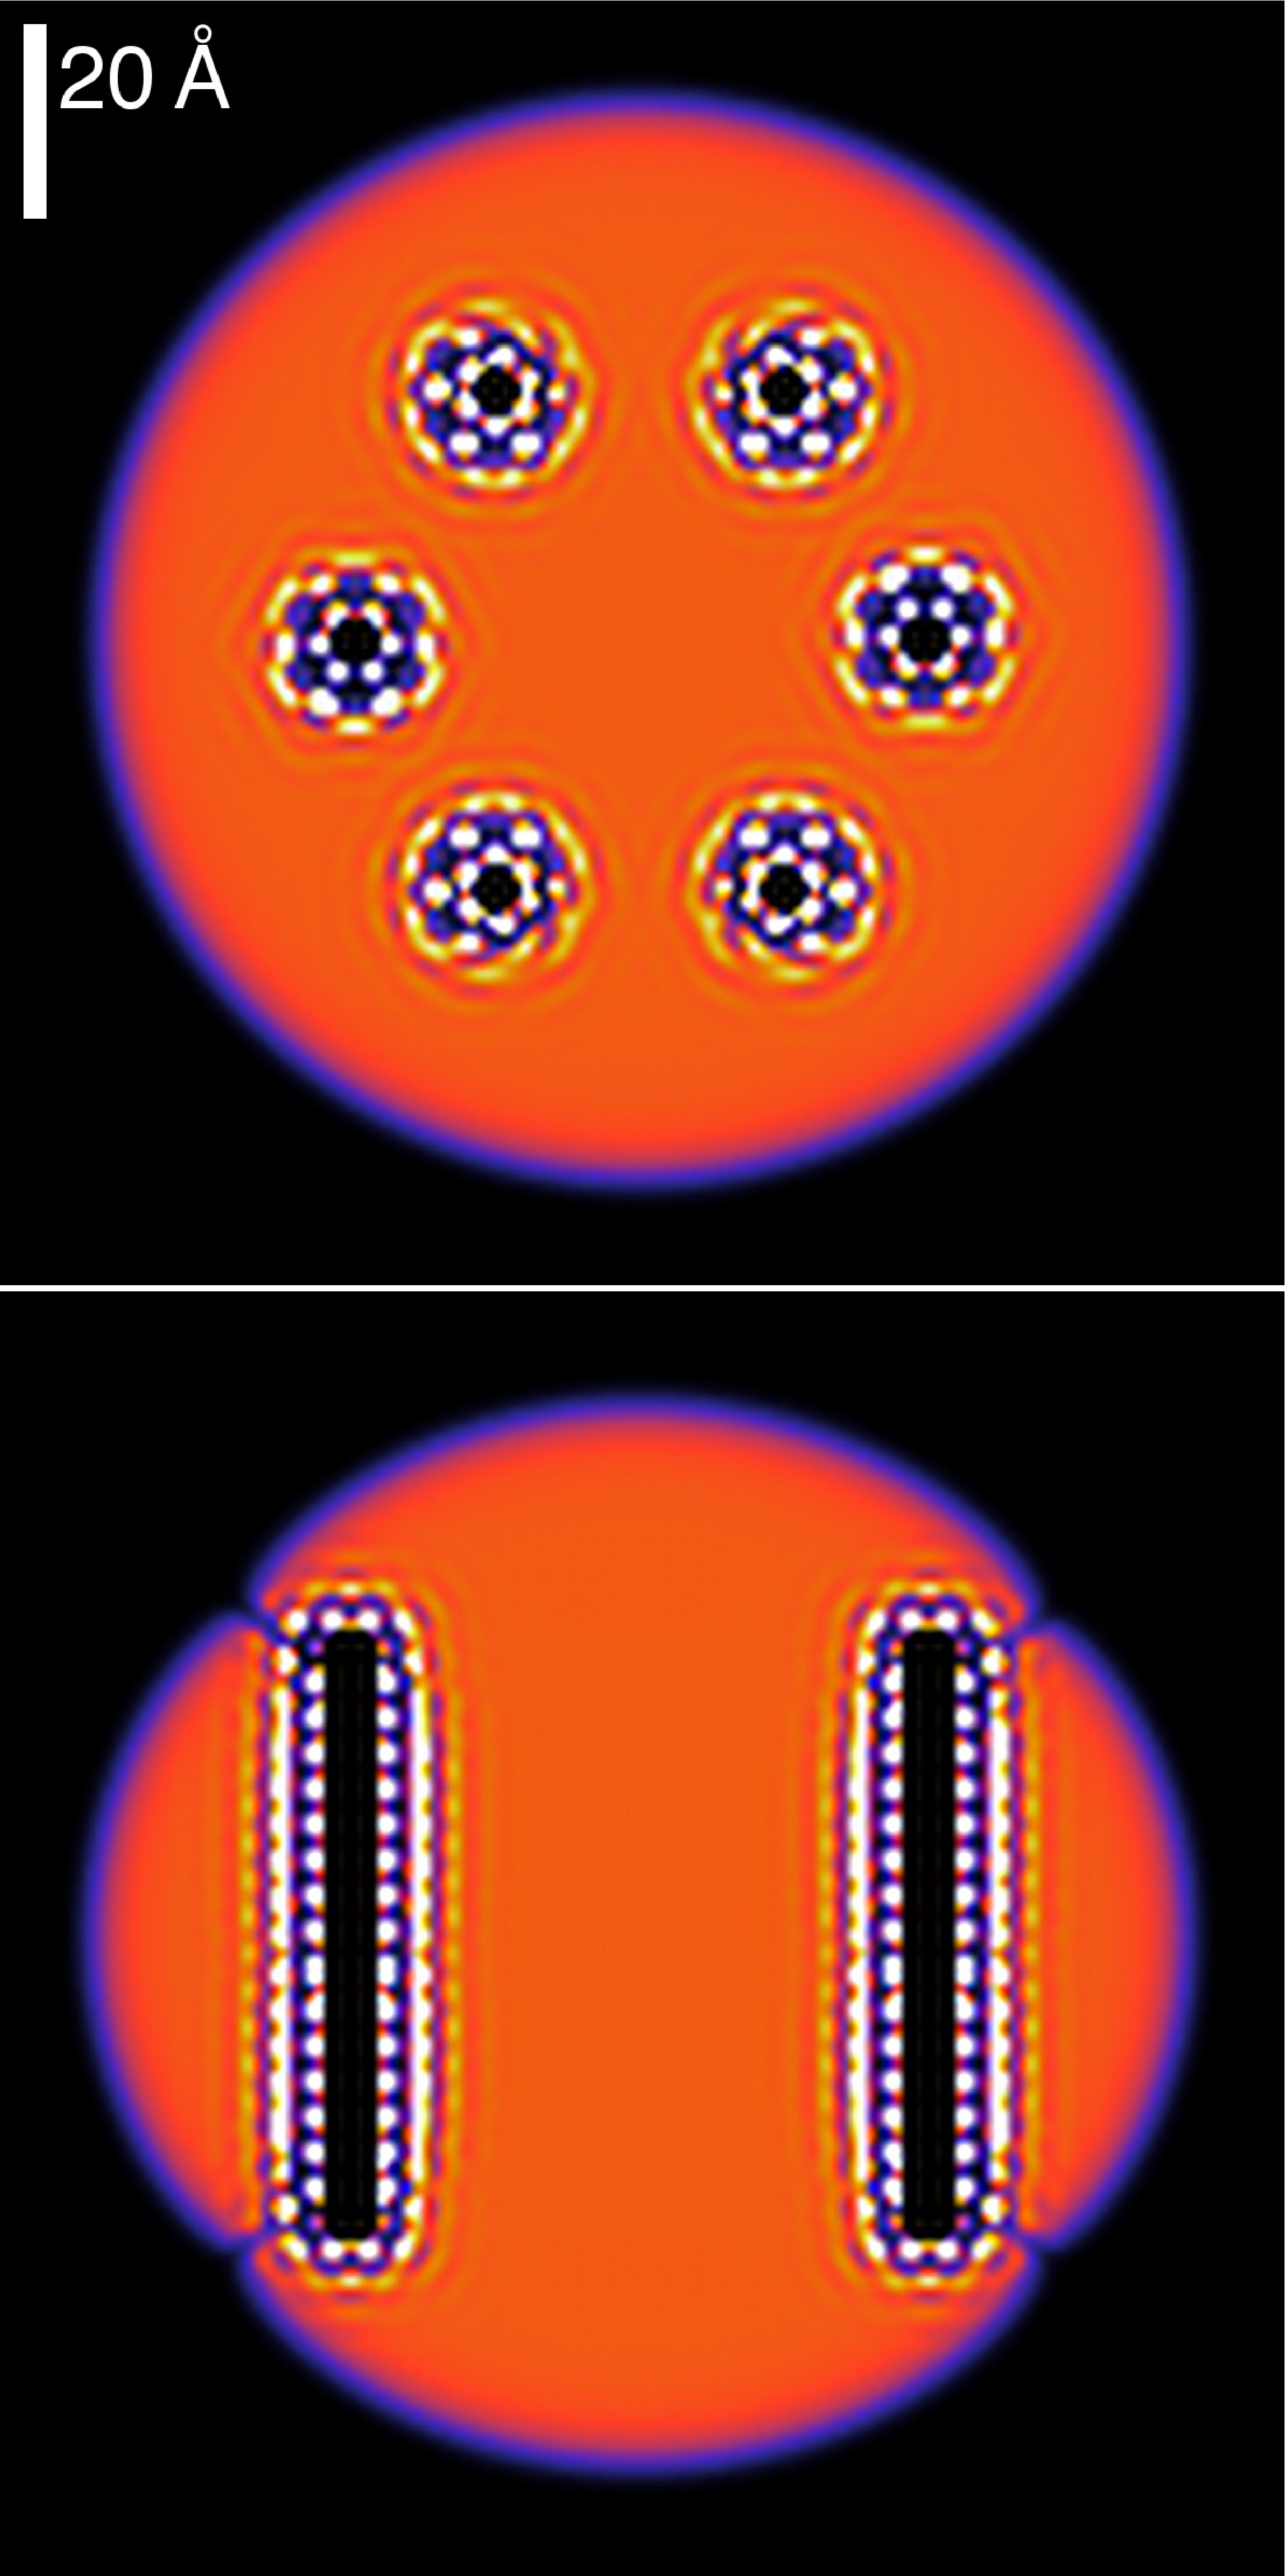
\includegraphics[width=0.6\linewidth,clip]{fig13}}
\caption{\label{fig13-capture} 
Helium droplet configuration hosting six vortices, each doped with a line of 
regularly spaced Ar atoms (not represented). 
The top figure shows the density in the $x-y$
symmetry plane (top view), while the bottom figure shows a side view corresponding to the 
$y-z$ plane. 
As in some of the previous figures, the bright  spots are high density blobs appearing around the impurity atoms.
}
\end{figure}

\begin{figure}[!]
\centerline{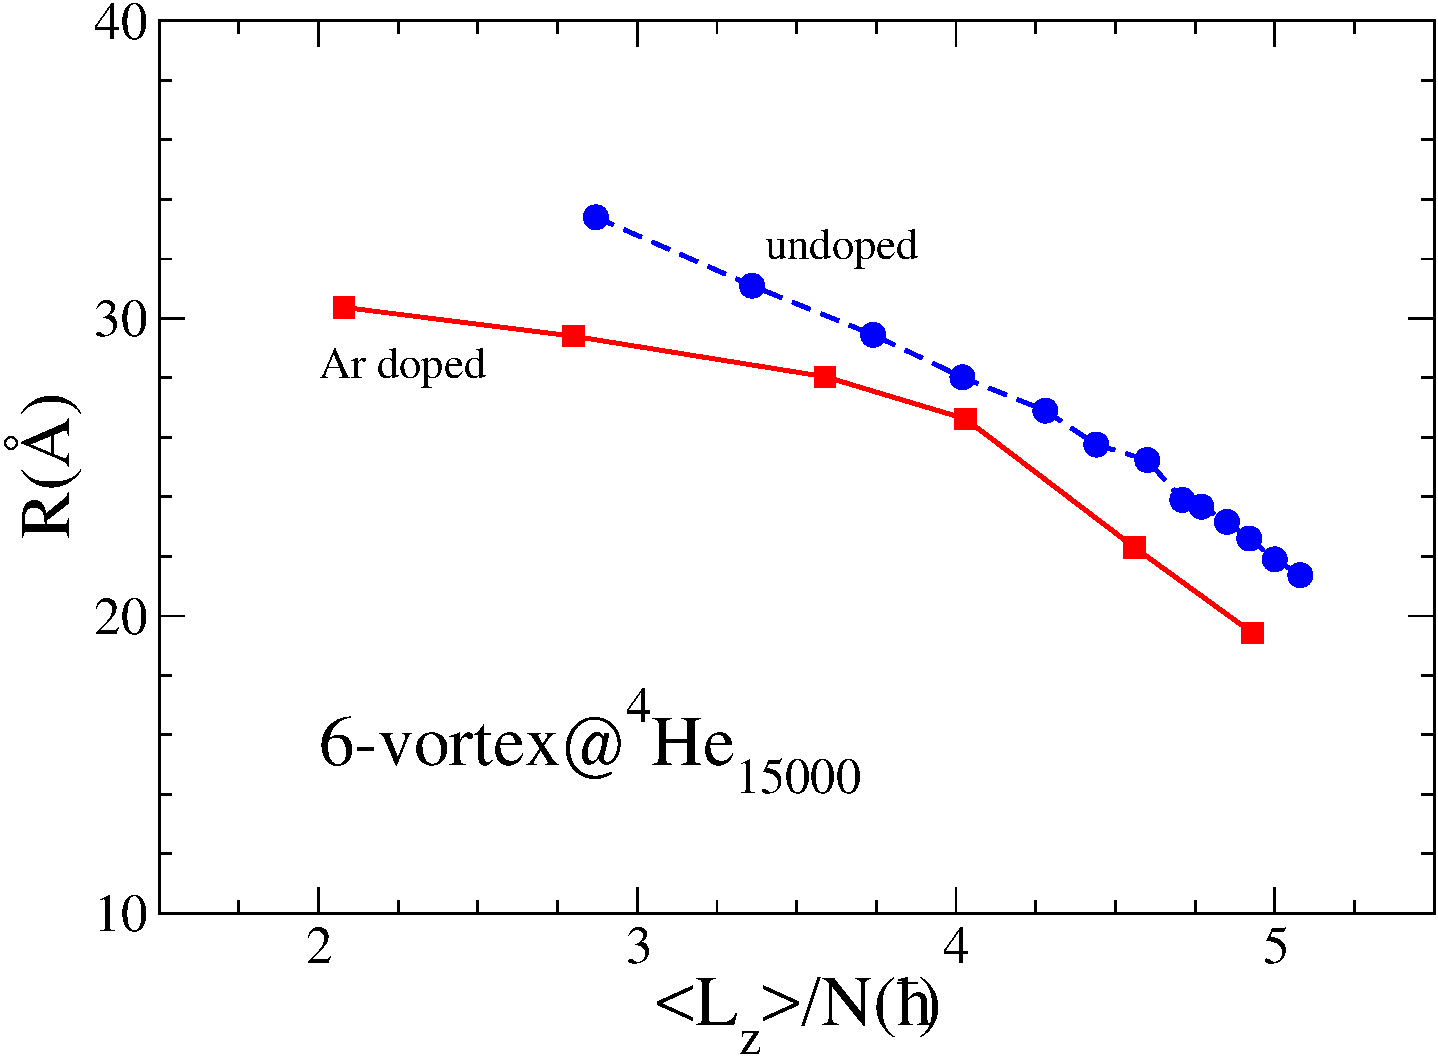
\includegraphics[width=0.9\linewidth,clip]{fig14}}
\caption{\label{fig14-capture} 
Calculated equilibrium distance of the 6-vortex ring
from the droplet center as a function of the 
angular momentum per He atom in units of $\hbar$. 
The dots represent the results for undoped vortices, while the squares are the results for 
Ar-doped vortices. The lines are drawn as a guide to the eye.
}
\end{figure}

In practice, as more and more Xe atoms become
attached to a vortex, they adopt the angular velocity of its
revolution about the droplet center. 
If the Xe capture is isotropic, the total angular momentum of the droplet is conserved, and 
thus the angular momentum accompanying the Xe rotational motion must be
transferred from the vortices to the impurities. This reduction in the angular momentum of the
vortices causes them to move outwards, 
resulting in the larger
equilibrium distances of the vortices observed in 
the experiments. The actual equilibrium radial positions
result from a balance between this tendency to 
move towards the droplet surface 
and the solvation potential, 
which tends instead to draw impurities towards the droplet
center.

We have looked for stationary configurations of a 6-vortex ring
in a rotating He$_{15000}$ droplet by solving the
EL equations in the corotating frame with a fixed
angular velocity. Each vortex core is filled with Ar
atoms, and the system is allowed to fully relax.
In the end, the column of atoms inside each vortex core reaches an equilibrium structure 
where the Ar atoms are separated by a distance which  is roughly that of the Ar dimer.
One such configuration is shown in  Fig. \ref{fig13-capture}. Note that 
the vortex cores are almost straight lines, whereas in an
undoped droplet rotating with the same velocity 
the vortex lines would be bent, 
as shown  e.g. in Fig. \ref{fig7-capture}.
The Ar atoms are not shown in the Figure.
The localized structures appearing in the vortex cores are 
regions of highly inhomogeneous, high  $^4$He density
resulting from the Ar-He attractive potential.
% and \ref{fig9-capture}.

The presence of impurities thus confers rigidity to the vortex lines,
preventing them from bending. Yet, the small segment of the vortex line free from impurities bends so as to hit 
the droplet surface perpendicularly, see the bottom Fig. \ref{fig13-capture}.
Note that in the absence of vortices, Ar atoms initially placed
in a linear chain structure would relax towards the lower energy, compact 
configuration of an Ar cluster in the bulk of the droplet.
However, once trapped by a vortex core, their collapse 
into such a cluster structure does not occur,
i.e. an energy barrier appears and prevents the formation of Ar
clusters. 
%As commented below, 
Our simplified 
description of the more complex experimental 
conditions (where each vortex line hosts chains of regularly spaced
atomic clusters, instead of chains of single atoms)
is due to computational limitations.

Our choice of Ar instead of Xe as a dopant is motivated by the weaker He-Ar and Ar-Ar interactions, which 
facilitates the imaginary-time relaxation. The interaction of the helium environment with several close-by impurities increases the 
strength of  dopant-droplet interaction, producing  
helium localization around the impurities (snowball structures), see Fig. \ref{fig10-capture}.  Stabilizing these
structures is extremely time consuming, 
especially when the He-impurity interaction is strong.
Experiments were also carried out with Ar atoms as dopants, 
but have not been analyzed yet.\citep{note}
However, no significant difference is expected between argon and xenon, 
neither from the experimental nor from the theoretical viewpoint.

There are obvious differences in scales between our simulations and  
 the actual experiments,  due to  computational 
cost. In experiments heavier impurities are used (Xe), 
the droplets are much larger
and the doping is known to occur by filling the vortex cores with a chain 
of equally spaced Xe clusters, each made of
hundreds of atoms, instead of atom chains as done in our simulations.
In spite of these differences, we find results which  
qualitatively explain the unusual behavior of vortex lines 
experimentally observed in doped rotating helium droplets.

We have looked for the equilibrium structure of the Ar@6-vortex $^4$He$_{15000}$ droplet
for different imposed values of the angular velocity
of rotation. The results show that the doping inside each vortex core
adds a substantial stability to the system, such that doped vortices are still 
stable in a droplet rotating at rather low 
values of the angular velocities, whereas undoped vortices
for such values would be pushed towards the surface of the
droplet and eventually expelled.
The solvation potential effect becomes
apparent below some critical 
value of the angular velocity, where the vortices
cease to move towards the surface and the 
system reaches an equilibrium maximum distance
of the vortices from the droplet center.
This is shown in the  Fig. \ref{fig14-capture}, 
where we plot the radial distance of the vortices
from the center as a function of the angular momentum
of the system.
Note how doped vortices are stable for values
of the angular momentum well below the stability 
limit of an undoped droplet.
A similar behavior has been observed in the experiment (see for instance Fig. 2 in the
Supplemental Material of ref. \citep{Jon16}).

%The issue of atomic or molecular impurities solvated within 
%$^4$He liquid droplets hosting quantized vortices is relevant  
%because of the experimental evidence that 
%quantized vortices in superfluid helium induce coalescence of solvated impurities,
%which become trapped along their cores. This 
%eventually results in the formation of nanosized filaments, thus 
%pointing to a   
%new potential method for producing nanowires. 
%Moreover, doping vortices with impurities has emerged as a 
%valuable practical tool to image the vortex positions and dynamics, especially 
%in the presence of vortex tangles and vortex reconnections.

%This has been the motivation of the present study, where
	\chapter{Conclusions \& Outlook}
	\section{Head-on collisions}
		In conclusion, head-on collisions of xenon, a heliophilic atom, involve a kinetic energy exchange of the same order of magnitude as cesium, a heliophobic atom with similar mass.
In both cases, this energy is largely dissipated by  producing energetic waves in the droplet or it is carried away by promptly emitted helium atoms.
The difference is that it takes a much higher velocity for xenon to go through the droplet and escape than for cesium, as could be expected.
Also, density builds up around the xenon during the dynamics, whereas a bubble is created around cesium.

	\section{Capture}
		We have shown
that Xe and Ar atoms at thermal velocities are readily captured by helium droplets, with a capture cross section similar to
 the geometric cross section of the droplet. Crucially for the subsequent capture of impurities by vortex lines,
we have also shown that most of the kinetic energy of the impinging impurity is lost in the capture process during the first tens of picoseconds. This happens either by the ejection of
 prompt-emitted He atoms, or by  the production of sound waves and large deformations in the droplet. 
 
If the droplet hosts a vortex,
slowly moving impurities are readily captured by the vortex line. 
Rather than being trapped inside the vortex core,
 the impurity is bound 
to move at a close distance around it.
Besides the crucial energy loss when the impurity hits the droplet,  the capture by the vortex is favored by a further
energy transfer  from the impurity to the droplet:  large amplitude 
displacements of the vortex line -- as shown in the ESI$\dag$ accompanying this work -- 
take place,  constituting another  source of the kinetic energy loss in the final stages of the capture.
A related issue is 
the appearance of Kelvin modes in the vortex line, that is not only bent,  but also twisted
in the course of the collision.

If the kinematic conditions of the collision (kinetic energy and impact parameter)  lead to the capture of the impurity by the droplet,   the pinball effect
caused by the droplet surface can induce
the meeting 
of the Xe/Ar atom and the vortex line -- and the possible capture of the atom by the vortex -- , since both have a tendency to remain in the inner region of the droplet. 
We have shown this in the case of Xe at $v_0=200$~m/s:
Xe is captured during its second transit across the droplet, whereas this could not have happened in bulk liquid helium.\cite{Psh16}  

The capabilities of the  He-DFT approach might help elucidate 
processes of experimental interest, such
as the capture of  one or several impurities 
by large droplets hosting a vortex  array and
how several atomic impurities, impinging upon a 
rotating droplet hosting vortices,  react 
to form small clusters, eventually being trapped within the 
vortex cores as it appears in the experiments.
		


\appendix
	\chapter{Angular velocity and angular momentum}

\lettrine[lines=3]{\color{activeColor}I}{n} this Appendix we discuss the relationship between angular velocity and angular momentum of a deformed droplet below the critical angular frequency for vortex 
nucleation.

Let us consider an ellipsoidal vessel filled with liquid $^4$He uniformly rotating around the $z$ axis, $\omega = \omega\, \hat{\mathbf{k}}$.
The ellipsoid has the equation
 %
$$ F(x,y,z) =\frac{x^2}{R_1^2}+ \frac{y^2}{R_2^2}+  \frac{z^2}{R_3^2} - 1 = 0$$
%
If $\mathbf{v}$ is the  irrotational velocity of a point in the laboratory, $\mathbf{v}'$ the velocity of the same point in the vessel (corotating frame),  and 
$\mathbf{V}= \omega \times \mathbf{r}$, one has
%
$$\mathbf{v}'=  \mathbf{v} - \mathbf{V} = \frac{\hbar}{m_4} \, \nabla {\cal S} - \omega \times \mathbf{r}$$
%
where ${\cal S}$ is the velocity potential defined here so as  that 
%
$$\mathbf{v}= \frac{\hbar}{m_4} \, \nabla {\cal S}(x,y,z)$$
%
Its existence is granted by irrotationality;  we also have
  $\mathbf{V}= \omega \times \mathbf{r} = \omega (-y,\, x, \,0)$.
A vector  perpendicular to the ellipsoid  surface is 
%
$\mathbf{n} = \nabla  F(x,y,z)$.
%
From the stationarity condition 
%
$( \mathbf{v}'  \cdot  \mathbf{n})|_{surf} =0$
%
one obtains
%
\begin{eqnarray}
&&\mathbf{v}'  \cdot  \mathbf{n}= 0 = \left.\left(\frac{\hbar}{m_4} \, \frac{\partial {\cal S}}{\partial x} + \omega y\right) \frac{x}{R_1^2} \right.
\nonumber
\\
\nonumber
&&
+  \left. \left(\frac{\hbar}{m_4} \,\frac{\partial {\cal S}}{\partial y} - \omega x\right) \frac{y}{R_2^2} 
+  \left(\frac{\hbar}{m_4} \, \frac{\partial {\cal S}}{\partial z} \right) \frac{z}{R_3^2} \right|_{surf}
\end{eqnarray}
%
It can be checked that ${\cal S} = \alpha xy$ is a solution to this equation provided that
%
$$\frac{\hbar}{m_4} \,  \left( \frac{1}{R_1^2}  + \frac{1}{R_2^2} \right)  \alpha = \left(\frac{1}{R_2^2}  - \frac{1}{R_1^2} \right)  \omega$$
%
Hence,
%
$$ \alpha = \frac{m_4}{\hbar}\,\left( \frac{R_2^2-R_1^2}{R_1^2+R_2^2}\right) \, \omega$$
%
and
%
$$ {\cal S} = \frac{m_4}{\hbar} \, \left( \frac{R_2^2-R_1^2}{R_1^2+R_2^2}\right)  \, \omega \, xy$$
%
The velocity in the laboratory is 
$ \mathbf{v} = (\hbar/m_4)\nabla {\cal S}=  (\hbar/m_4)\alpha (y, x, 0) $,
and in the vessel (corotating frame) is
$\mathbf{v}'= \beta (R_1^2 y, \, -R_2 ^2 x, \,0) $, where $\beta \equiv  2 \, \omega/(R_1^2+R_2^2)$.
 Once they have been determined, their  circulation lines are straightforwardly obtained. 
In the laboratory frame they are
$$ x^2 - y^2 = c \quad ,$$
%
which is the appearance of the circulation lines displayed in \fig{fig8-capture}. In the vessel  frame, they are
%
$$ \frac{x^2}{(\xi R_1)^2}+ \frac{ y^2}{(\xi R_2)^2} = 1 \quad .$$ 
%
These lines are ``parallel'' to the ellipsoidal surface.

We define the deformation parameter $\epsilon$
%
$$
\epsilon =\frac{\langle x^2 \rangle - \langle y^2 \rangle}{\langle x^2 \rangle + \langle y^2 \rangle}
$$
%
where e.g., 
$$ \langle x^2 \rangle = \frac{1}{N} \int d\mathbf{r} \,  x^2 \,\Psi(\mathbf{r}) $$
%
For the sharp surface ellipsoid above,
%
\begin{equation}
 \alpha = \frac{m_4}{\hbar} \, \epsilon \, \omega
 \label{eps}
 \end{equation}
%
This relationship is not  general but  can be used as a guide for our more general approach.
Let us  now discuss the angular momentum and moment of inertia of the irrotational fluid droplet. Recalling that
%
$$L_z = - \imath \; \hbar \left( x \frac{\partial}{\partial y} -  y \frac{\partial}{\partial x}\right)$$
%
if we write 
%
$$\Psi(\mathbf{r}) = \Phi(\mathbf{r}) e^{\imath \alpha xy}$$
%
with $\Phi(\mathbf{r})$ a real function,
%
$$\langle L_z \rangle = \hbar\,  \alpha  \int d\mathbf{r} \,  (x^2-y^2)  \,\Phi^2(\mathbf{r})$$
%
If \eq{eps} holds,
%
\begin{eqnarray}
&&\langle L_z \rangle = \epsilon \, m_4 N  [\langle x^2 \rangle - \langle y^2\rangle]\, \omega   
\nonumber
\\ 
&& = m_4  N \left( \frac{[\langle x^2 \rangle - \langle y^2\rangle ]^2}{\langle x^2 \rangle + \langle y^2\rangle} \right)\, \omega  \equiv  {\cal I}_{irr} \, \omega
 \label{irrot}
\end{eqnarray}
%
where 
%
$$ {\cal I}_{irr} = m_4 N \left( \frac{[\langle x^2 \rangle - \langle y^2\rangle ]^2}{\langle x^2 \rangle + \langle y^2\rangle} \right)$$
%
is the irrotational moment of inertia. For a rigid solid,
%
$$  {\cal I}_{rig} =  m_4  \int d\mathbf{r} \,  (x^2+y^2)  \,\Phi^2(\mathbf{r}) = m_4 N [\langle x^2 \rangle + \langle y^2\rangle] $$
%
Hence, 
%
$$ \frac{{\cal I}_{irr}}{{\cal I}_{rig}} = \left[ \frac{\langle x^2 \rangle - \langle y^2\rangle }{\langle x^2 \rangle + \langle y^2\rangle} \right]^2 \rightarrow 0 \quad {\rm if} \quad \epsilon \rightarrow 0$$
%
Finally, we discuss the kinetic energy of the droplet
%
$$ E_{kin} = \frac{\hbar^2}{2 m_4}  \int \, d\mathbf{r} \,|\nabla \Psi(\mathbf{r})|^2$$
%
From the above $\Psi(\mathbf{r})$, 
%
\begin{eqnarray}
&&E_{kin}= \frac{\hbar^2}{2 m_4}  \int \, d\mathbf{r} \,|\nabla \Phi(\mathbf{r})|^2
\nonumber
\\
\nonumber
&+& \frac{\hbar^2}{2 m_4} \alpha^2 \int \, d\mathbf{r} \, (x^2 + y^2) \Phi^2(\mathbf{r})= E_{intr}+E_{coll}
\end{eqnarray}
%
where the first term is the ``intrinsic'' kinetic energy and the second term arises from the irrotational velocity field
%
\begin{eqnarray}
&&E_{coll}= \frac{\hbar^2}{2 m_4} \alpha^2 \int  d\mathbf{r} \, (x^2 + y^2) \Phi^2(\mathbf{r}) =
\nonumber
\\
\nonumber
&& \frac{1}{2} \left\{ m_4\, \epsilon^2 \int d\mathbf{r} \, (x^2 + y^2) \Phi^2(\mathbf{r})\right\} \omega^2= \frac{1}{2}\, {\cal I}_{irr} \,\omega^2
 \end{eqnarray}
% 

 These expressions may be used to obtain some estimates from the actual DFT calculations.
 For  a $^4$He$_{1000}$ droplet and $\omega$=0.10 K/$\hbar$ 
 we have obtained $\langle x^2\rangle$= 100.82 \AA$^2$ and  $\langle y^2\rangle$= 101.82 \AA$^2$; hence,
 $\epsilon \sim -1/200$. Since $\hbar^2/m_4$= 12.12 K \AA$^2$, from \eq{eps} one has $\alpha \sim -4.2 \times 10^{-5}$ \AA$^{-2}$. 
From \eq{irrot} we obtain  $\langle L_z\rangle \sim 4 \times 10^{-2} \, \hbar$.
  
 In a Bose-Einstein condensate  the deformation $\epsilon$ is a control parameter that can be set to a very large value (close to unity). For a self-bound $^4$He droplet deformation comes from
 ``rotation'' itself and it turns out to be minute
  even for angular frequencies close to the critical frequency  for one-vortex nucleation; the conclusion is that the droplet ``does not rotate'';
 in other words, it is unable to store an appreciable amount of angular momentum before vortex  nucleation.


\backmatter
	\addcontentsline{toc}{chapter}{Bibliography}
\bibliographystyle{apsrev}
\bibliography{references,review_refs}

\end{document}